% Waveform analysis for the PRad-II / X17 HyCal data (branch waveform_jz).
% Section -> script map (paths relative to analysis/pyscripts):
%   3, 4   waveform_analysis/template_extract.py
%   5.1    class MF in waveform_analysis/pileup_analysis/pileup_deconvolution_study.py
%          (same class in pileup_rates.py, crosstalk_study.py, energy_resolution_benchmark.py)
%   5.2    waveform_analysis/pileup_analysis/pileup_rates.py (scan, report)
%   5.3    waveform_analysis/pileup_analysis/pileup_generator_stage1.py
%   5.4    waveform_analysis/pileup_analysis/pileup_deconvolution_study.py
%   6      waveform_analysis/pileup_analysis/exotic_events/exotic_p1_quantities.py ... exotic_p13_drop_flagged.py (exotic_p13_recluster.py),
%          exotic_p7_saturated_seeds.py, exotic_summary.py (front matter = numbers quoted); scan option PILEUP_EXOTIC=1 of pileup_rates.py;
%          P9 and P13 run energy_resolution_benchmark.py / moller_calib.py with the opt-in EXOTIC_HOOK (default path = v3)
%   6 figs writeup/make_figs/exotic_events_figs.py (figs/exotic_events/exotic_*.pdf)
%   7      crosstalk_study/crosstalk_study.py (scan, report)
%   9      waveform_analysis/energy_resolution_benchmark.py (working tree of 14 Nov 2026, control v3 defaults)
%          tables: waveform_analysis/energy_resolution/improvement/control_phase2_v3*.tsv, P*.md
%   9 figs writeup/make_figs/calib_figs.py (calib_*.pdf; run from analysis/pyscripts)
\documentclass[11pt]{article}
\usepackage[a4paper,margin=25mm]{geometry}
\usepackage{amsmath}
\usepackage{amssymb}
\usepackage{booktabs}
\usepackage{graphicx}
\graphicspath{{figs/}{figs/exotic_events/}}
\usepackage[colorlinks=true,linkcolor=blue,urlcolor=blue]{hyperref}

\newcommand{\ns}{\,\mathrm{ns}}
\newcommand{\adc}{\,\mathrm{ADC}}
\newcommand{\mev}{\,\mathrm{MeV}}
\newcommand{\code}[1]{\texttt{#1}}
\DeclareMathOperator*{\argmin}{arg\,min}
\DeclareMathOperator*{\argmax}{arg\,max}
\DeclareMathOperator{\median}{median}
\DeclareMathOperator{\MAD}{MAD}
\DeclareMathOperator{\sgn}{sgn}

\title{Waveform Analysis for PRad-II/X17}
\author{Jingyi Zhou}
\date{\today}

\begin{document}
\maketitle
\tableofcontents
\clearpage

\section{Introduction and roadmap}
\label{sec:intro}

This note documents the waveform-level analysis of the HyCal calorimeter data taken for PRad-II and for the X17 search. It starts from the flash-ADC samples of each channel and ends at the pulse onsets and amplitudes that enter the cluster energy. Each part states its purpose, inputs and outputs, lists the procedure as numbered steps with the constants of the code, and closes with the results on disk. Every number quoted for a run type comes from an output file of the scripts of Table~\ref{tab:scripts}, except where the text names another source.

The parts build on each other in the following order.
\begin{enumerate}
\item \textbf{Data and notation} (Section~\ref{sec:data}): detector, readout, trigger gate, runs and the symbols of the whole note.
\item \textbf{Pulse selection} (Section~\ref{sec:selection}): clean single pulses are selected per module.
\item \textbf{Pulse templates} (Section~\ref{sec:templates}): a cubic-spline pulse shape and its pulse-to-pulse scatter are fitted per module and run type.
\item \textbf{Pile-up fitter} (Section~\ref{sec:fitter}): the templates are fitted to a waveform with up to six pulses, which gives the onset and amplitude of each pulse.
\item \textbf{Pile-up rates and hot modules} (Section~\ref{sec:rates}): the fitter runs on data, and the channels and clusters with a second pulse are counted per run type and per module.
\item \textbf{Pile-up generator} (Section~\ref{sec:generator}): one- and two-pulse waveforms with known truth are generated from the templates.
\item \textbf{Deconvolution study} (Section~\ref{sec:deconv}): the fitter runs on the generated waveforms; its efficiency, false-positive rate and amplitude bias are measured against the truth.
\item \textbf{Exotic waveforms} (Section~\ref{sec:exotic}): waveforms that are not a sum of template pulses are flagged in five categories, counted per run type, module and cluster, and their cost in the elastic yields is measured.
\item \textbf{Crosstalk study} (Section~\ref{sec:xtalk}): fit quality and timing of cluster members isolate a late signal induced by the neighbouring digitizer channel.
\item \textbf{Summary} (Section~\ref{sec:summary}): the key numbers of parts 2 to 5, 7 and 9 in one table, and the open points.
\item \textbf{Energy calibration} (Section~\ref{sec:calib}): the calibration chain built on the fitted amplitudes, step by step, the comparison of its states and the present resolution.
\end{enumerate}

\begin{table}[htbp]
\centering
\caption{Scripts and main outputs of each part. Paths are relative to \code{analysis/pyscripts}; \code{<RT>} stands for the run type.}
\label{tab:scripts}
\small
\begin{tabular}{lp{0.40\textwidth}p{0.36\textwidth}}
\toprule
Part & Script & Main output \\
\midrule
Selection, templates & \code{waveform\_analysis/template\_extract.py} & \code{templates\_<RT>.npz} (template bank) \\
Fitter & class \code{MF} in \code{pileup\_deconvolution\_study.py} & none (called by the scripts below) \\
Rates, hot modules & \code{pileup\_analysis/pileup\_rates.py} & \code{pileup\_rates\_out/} (tables, PDF pages) \\
Generator & \code{pileup\_analysis/pileup\_generator\_stage1.py} & \code{pileup\_stage1.npz} \\
Deconvolution study & \code{pileup\_analysis/pileup\_deconvolution\_study.py} & \code{efficiency.tsv}, two PDF files \\
Exotic waveforms & \code{pileup\_analysis/exotic\_events/exotic\_p1\_quantities.py} to \code{exotic\_p13\_drop\_flagged.py} & \code{exotic\_events/exotic\_P<n>\_*.tsv}, \code{exotic\_summary\_20261118.pdf} \\
Crosstalk & \code{crosstalk\_study/crosstalk\_study.py} & \code{crosstalk\_study/out/} \\
Calibration & \code{waveform\_analysis/energy\_resolution\_benchmark.py} & resolution tables \\
\bottomrule
\end{tabular}
\end{table}

\section{Data and notation}
\label{sec:data}

\subsection{Detector, readout and trigger}
\label{sec:detector}

HyCal has a central part of 1152 PbWO$_4$ modules (W1 to W1156; $20.77 \times 20.75 \times 180$\,mm$^3$) surrounded by 576 lead-glass modules (names starting with G; $38.15 \times 38.15 \times 450$\,mm$^3$). Four PbWO$_4$ positions at the centre are empty and form the $2 \times 2$ hole for the beam. The ring index of a PbWO$_4$ module is $\lfloor \max(|x|, |y|)/d \rfloor$, with $(x, y)$ the module centre and $d$ the module size; ring 1 holds the 12 modules around the hole.

Every channel is digitised by a 250\,MHz flash ADC with 12-bit range. An event holds 100 samples at a 4\,ns period (400\,ns) per channel, and a sample at 4095\,ADC is clipped. The readout is zero-suppressed, so an event contains only the channels above the readout threshold.

The trigger word \code{trigger\_bits} carries the raw-sum trigger in bit 8 (\code{0x100}), three cluster triggers in bits 9 to 11 and the Light Monitoring System (LMS), a laser flash that illuminates all channels, in bit 24 (\code{0x1000000}). The selection, the pile-up scan and the crosstalk scan apply one event gate: hydrogen run types require \code{trigger\_bits} $=$ \code{0x100} exactly, the tantalum run type requires at least one of bits 8 to 11, and LMS events are dropped. The run-information file \code{database/runinfo/general.json} gives for each run the beam energy $E_b$, the calibration file with the constants $c_m$ and the list of dead modules.

\subsection{Runs}
\label{sec:runs}

Table~\ref{tab:runs} lists the runs of the pile-up scan of Section~\ref{sec:rates}. The crosstalk scan of Section~\ref{sec:xtalk} uses the hydrogen runs of the table, and Section~\ref{sec:calib} uses all of them plus three earlier 3.49\,GeV runs. A template bank exists for each run type of the table.

\begin{table}[htbp]
\centering
\caption{Run types and runs. Files is the number of raw-data files read; Events is the number of events after the trigger gate and the LMS veto in the pile-up scan. The dead module W1141 of \code{3p49GeV\_H2} applies from run 24850 on.}
\label{tab:runs}
\small
\begin{tabular}{lp{0.19\textwidth}llll}
\toprule
Run type & Runs & $E_b$ (MeV) & Files & Events & Dead modules \\
\midrule
\code{0p73GeV\_H2} & 24590, 24603 & 728.9 & 16 & 3\,133\,150 & W691, W1019, W1020, W1124 \\
\code{2p24GeV\_H2} & 25228, 25257, 25260, 25299, 25320 & 2239.51 & 42 & 6\,702\,649 & W1019, W1020, W1124 \\
\code{3p49GeV\_H2} & 24698, 24911, 24937 & 3485.41 & 20 & 2\,546\,884 & W1019, W1020, W1124, W1141 \\
\code{2p24GeV\_Ta\_X17} & 25800, 26138, 26230 & 2239.51 & 25 & 2\,520\,012 & W781, W1019, W1020, W1124 \\
\bottomrule
\end{tabular}
\end{table}

\subsection{Notation}
\label{sec:notation}

Each PbWO$_4$ channel is read out as 100 flash-ADC samples at a 4\,ns period. The symbols below are used throughout; every other symbol is defined where it first appears. In Sections~\ref{sec:selection} and \ref{sec:templates} the index $i$ labels a selected pulse, one per waveform. From Section~\ref{sec:pileup} on a waveform can hold several pulses: the waveform index is dropped, $n$ labels the pulses of the waveform, and Table~\ref{tab:notation} lists these symbols in its second block.

\begin{table}[htbp]
\centering
\caption{Symbols. First block: Sections~\ref{sec:selection} and \ref{sec:templates}; second block: symbols added from Section~\ref{sec:pileup} on.}
\label{tab:notation}
\small
\begin{tabular}{lp{0.72\textwidth}}
\toprule
Symbol & Meaning \\
\midrule
$s_{ij}$ & raw ADC sample $j = 0,\dots,99$ of pulse $i$ \\
$t_j = 4j\ns$ & sample time \\
$p_i$, $r_i$ & WaveAnalyzer pedestal and pedestal rms of pulse $i$ (ADC) \\
$n_{\mathrm{ped}}$ & number of samples in the WaveAnalyzer pedestal window \\
$w_{ij} = s_{ij} - p_i$ & baseline-subtracted sample \\
$k_i$ & peak sample, the first index at which $w_{ij}$ reaches its maximum \\
$A_i$ & pulse amplitude; at selection $A_i^{\mathrm{raw}} = w_{ik_i}$, in the fit the fitted amplitude \\
$\sigma_i = \max(r_i,\,0.3\adc)$ & per-sample noise of pulse $i$ (\code{SIG\_MIN}) \\
$E_b$ & beam energy (MeV); $c_m$ the calibration constant of module $m$ (MeV per ADC sample) \\
$t_{0,i}$ & pulse onset (ns); $t^{\mathrm{cfd}}_i$ its first estimate from a constant-fraction crossing \\
$\tau_{ij} = t_j - t_{0,i}$ & sample time relative to the onset \\
$f(\tau)$ & unit-peak template of a module; $f_{\mathrm{ref}}$ the template of the previous fit pass \\
$\lambda$ & smoothing parameter of the spline fit \\
\midrule
$s_j$, $y_j = s_j - \bar p$ & samples of one waveform, raw and baseline-subtracted; $\bar p$ the baseline estimate, $\delta p$ its fitted offset \\
$\omega_j$ & sample weight: 0 for a clipped sample ($s_j \ge 4095$), 1 otherwise \\
$\sigma$, $\sigma_{\mathrm{ref}}$ & per-sample noise of a waveform; reference noise of a module in one file \\
$A_n$, $t_{0,n}$ & amplitude (ADC above the baseline) and onset (ns after sample 0) of pulse $n = 1,\dots,K$; $K \le 6$ \\
$\hat y_j$ & fitted model at sample $j$, Eq.~\eqref{eq:model} \\
$N$, $D$, $S$, $\hat A$, $\sigma_A$ & matched-filter sums, score, amplitude estimate and its error at a trial onset, Eq.~\eqref{eq:mf} \\
$A_{\mathrm{thr}}$ & detection threshold, Eq.~\eqref{eq:athr} \\
$\sigma_s(\tau)$, $a_{\mathrm{band}}$ & shape scatter of the template (\code{shape\_sigma}) and the amplitude at which it was measured (\code{a\_band}) \\
$V_j$ & variance of sample $j$, Eq.~\eqref{eq:vj} \\
$t_{\mathrm{pk}}$, $t_{50}$ & peak time and half-maximum time of the template after its onset (\code{t\_pk}, \code{t50}) \\
$A_{\mathrm{main}}$ & largest fitted amplitude of a channel (main pulse) \\
$\rho$, $\Delta t$ & amplitude ratio and onset difference of a second pulse relative to the main or primary pulse \\
$I_m$, $g_m = c_m I_m$ & WaveAnalyzer integral of the unit-peak template (\code{iint\_wa}); gain of module $m$ (MeV per ADC of amplitude) \\
$E_{\mathrm{main}} = g_m A_{\mathrm{main}}$, $E$ & energy of the main pulse; cluster energy \\
$F$, $\varepsilon$ & rate (fraction of channels or clusters); efficiency \\
$A_1$, $A_2$, $t_1$, $t_2$ & generated amplitudes and onsets of the primary and the secondary pulse; a hat marks the fitted value compared with them \\
$\delta f(\tau)$, $\alpha$ & per-event perturbation of the template in the generator and its scale factor \\
$\delta t$ & constant-fraction time minus matched-filter time of a pulse, Eq.~\eqref{eq:dtcfd} \\
$\theta$, $r_\perp$, $E'$ & polar angle and radial distance of a cluster seed from the beam axis; elastic reference energy \\
$G_m$, $H(\xi, \eta)$ & gain factor of the gain solve; position correction, Eqs.~\eqref{eq:gainsolve} and \eqref{eq:poscorr} \\
\bottomrule
\end{tabular}
\end{table}

\section{Pulse selection}
\label{sec:selection}

Selection runs on the decoded events of one run and stores, for each surviving pulse, its 100 samples, pedestal, rms, amplitude, peak sample, onset estimate and rough energy. The event-level gates come first; the per-pulse cuts follow in the order of Table~\ref{tab:cuts}.

\subsection{Event-level gates}

An event enters the selection when all of the following hold.
\begin{enumerate}
\item \textbf{Trigger.} Run types with the \code{physics} trigger rule require $\code{trigger\_bits} = \code{0x100}$ exactly; run types with \code{physics-any} require $(\code{trigger\_bits}\ \&\ \code{0xf00}) \neq 0$.
\item \textbf{No LMS.} An event with bit \code{0x1000000} set in \code{trigger\_bits} is dropped (\code{EXCLUDE\_TRIGGER\_BITS}).
\item \textbf{Channel.} Only channels mapped to a HyCal PbWO$_4$ module that is not in the dead list, with exactly 100 samples, are kept.
\item \textbf{Busy event.} Over the channels of the event, count those with $\max_j s_{ij} - p_i \ge 50\adc$ (\code{MODULE\_COUNT\_HEIGHT\_MIN}). If more than 20 channels qualify (\code{MAX\_MODULES\_PER\_EVENT}) the whole event is dropped. This count uses the raw maximum, so clipped channels are included, and the gate precedes the clipping cut.
\end{enumerate}

\subsection{Per-pulse cuts}

The pedestal $p_i$ and rms $r_i$ are the WaveAnalyzer values of the pulse itself. The cuts of Table~\ref{tab:cuts} are boolean masks combined by logical AND, so the set of surviving pulses does not depend on their order; the order fixes only the cumulative cut-flow counters.

\begin{table}[htbp]
\centering
\caption{Per-pulse selection cuts in code order. $A_i = A^{\mathrm{raw}}_i$ throughout this table.}
\label{tab:cuts}
\small
\begin{tabular}{llll}
\toprule
\# & Cut & Condition & Constant \\
\midrule
1 & no clipping & $\max_j s_{ij} < 4095$ & \code{CLIP\_ADC} \\
2 & amplitude & $A_i = \max_j s_{ij} - p_i \ge 50\adc$ & \code{A\_STORE\_MIN} \\
3 & contained & $k_i \le 59$ & \code{PEAK\_MAX\_SAMPLE} \\
4 & pre-pulse window & $j^{\mathrm{thr}}_i \ge 20$ & \code{PRE\_SAMPLES}, \code{THR\_ADC} \\
5 & pedestal quality & $r_i \le 1.5\adc$ and $|b_i| \le 0.05\adc/\text{sample}$ & \code{PED\_RMS\_MAX}, \code{PED\_SLOPE\_MAX} \\
6 & tail level & $|\bar w^{\mathrm{tail}}_i| \le \max(2\adc,\,2r_i) + 0.04\,A_i$ & \code{TAIL\_*} \\
7 & no secondary bump & $\beta_i < 0.10\,A_i$ & \code{SEC\_FRAC} \\
8 & smoothness & rising edge monotone, tail steps $\le 2 r_i$ & \code{TAIL\_NSAMP}, \code{NOISE\_ALLOW} \\
9 & energy & $e^{\mathrm{rough}}_i < 1.2\,E_b$ & \code{EMAX\_FRAC} \\
\bottomrule
\end{tabular}
\end{table}

The quantities in the table are defined as follows. Cuts 4 to 8 act on $w_{ij}$, computed for the pulses that passed cuts 1 to 3.

\paragraph{Pre-pulse window (cut 4).} $j^{\mathrm{thr}}_i$ is the first sample at or before the peak that exceeds 2\,ADC above the pedestal:
\begin{equation}
j^{\mathrm{thr}}_i = \min\{\, j \le k_i : w_{ij} > 2\adc \,\}.
\end{equation}
Requiring $j^{\mathrm{thr}}_i \ge 20$ guarantees 20 pre-pulse samples.

\paragraph{Pedestal quality (cut 5).} The pre-pulse slope $b_i$ is the least-squares slope of the 20 samples before $j^{\mathrm{thr}}_i$,
\begin{equation}
b_i = \frac{\sum_{l=0}^{19} x_l\, w_{i,\,j^{\mathrm{thr}}_i - 20 + l}}{\sum_{l=0}^{19} x_l^2},
\qquad x_l = l - 9.5,
\end{equation}
in ADC per sample. The slope is evaluated only for pulses that passed cut 4.

\paragraph{Tail level (cut 6).} $\bar w^{\mathrm{tail}}_i$ is the mean of $w_{ij}$ over the samples $k_i + 40 \le j \le \min(k_i + 50,\, 99)$ (\code{TAIL\_OFF0}, \code{TAIL\_OFF1}). The tolerance $\max(2\adc, 2r_i) + 0.04\,A_i$ combines the noise floor with a 4\,\% allowance for the pulse's own tail (\code{TAIL\_ABS\_ADC}, \code{TAIL\_RMS\_MULT}, \code{TAIL\_FRAC\_A}).

\paragraph{Secondary bump (cut 7).} $\beta_i$ is the largest rise of any post-peak sample above the lowest sample seen since the peak,
\begin{equation}
\beta_i = \max_{j > k_i}\Big[\, w_{ij} - \min_{k_i \le l \le j} w_{il} \,\Big].
\end{equation}
A pile-up pulse in the tail raises $\beta_i$ by its own amplitude; the cut rejects anything above 10\,\% of $A_i$.

\paragraph{Smoothness (cut 8).} Let $j^{\mathrm{edge}}_i = 1 + \max\{ j < k_i : w_{ij} \le 2\adc \}$ be the sample after the last sub-threshold sample before the peak. The rising edge must not decrease,
\begin{equation}
w_{i,j+1} \ge w_{ij} \quad \text{for } j^{\mathrm{edge}}_i \le j < k_i,
\end{equation}
and over the eight samples after the peak no sample may rise above its predecessor by more than twice the noise,
\begin{equation}
w_{i,j+1} - w_{ij} \le 2\,r_i \quad \text{for } k_i \le j < k_i + 8 .
\end{equation}

\paragraph{Onset and rough energy.} For the pulses that passed cuts 1 to 8 the constant-fraction onset is the linearly interpolated time at which the rising edge first reaches half the amplitude (\code{CFD\_FRAC}),
\begin{equation}
t^{\mathrm{cfd}}_i = 4\ns\,\Big[(q-1) + \frac{0.5\,A_i - w_{i,q-1}}{w_{iq} - w_{i,q-1}}\Big],
\qquad q = \min\{\, j : w_{ij} \ge 0.5\,A_i \,\}.
\label{eq:cfd}
\end{equation}
The rough energy sums the baseline-subtracted samples from three samples before the onset sample to the end of the window (\code{E\_PRE}),
\begin{equation}
e^{\mathrm{rough}}_i = c_m \sum_{j \ge \lfloor t^{\mathrm{cfd}}_i / 4\ns \rfloor - 3}^{99} w_{ij}.
\label{eq:erough}
\end{equation}
Cut 9 keeps $e^{\mathrm{rough}}_i < 1.2\,E_b$.

\paragraph{Cut flow.} Per module, the selection records the number of pulses surviving each cut cumulatively in code order. No per-module cap is applied at selection. Pile-up is removed only by the shape cuts 6 to 8.

\section{Pulse templates}
\label{sec:templates}

The template of a module is the mean shape of its pulses, with unit peak and time zero at the onset. It is built per run type from the selected pulses of Section~\ref{sec:selection} and stored in the template bank, together with the pulse-to-pulse scatter of the shape. The fitter of Section~\ref{sec:fitter}, the generator of Section~\ref{sec:generator} and the energy estimator of Section~\ref{sec:calib} read the bank.

The build of one module runs through the following steps.
\begin{enumerate}
\item Choose the fit pool of the module (Section~\ref{sec:pools}).
\item Subtract the baseline, align and normalise each pooled pulse (Section~\ref{sec:prep}).
\item Fit a penalised cubic spline to the pooled points, realign every pulse to the result and repeat (Sections~\ref{sec:model} and \ref{sec:fit}).
\item Measure the error of the mean shape and the pulse-to-pulse scatter (Section~\ref{sec:unc}).
\item Assign the run-type average to a module without a usable pool (Section~\ref{sec:fallback}).
\item Write the bank (Section~\ref{sec:outputs}).
\end{enumerate}

\subsection{Fit pool per module}
\label{sec:pools}

The template of module $m$ is fitted to a pool of its selected pulses. Pulses are sorted by $e^{\mathrm{rough}}$ in descending order, and one random generator per module, seeded with $(1, m)$ (\code{SEED}), draws every random subset. Let $n_{\mathrm{el}}$ be the number of pulses with $e^{\mathrm{rough}} \ge 0.5\,E_b$ (\code{POOL\_EFRAC}): the seed crystal of an elastic cluster holds about 70\,\% of the energy. The candidate pools are tried in the following order until the fit of Section~\ref{sec:fit} succeeds.

\begin{enumerate}
\item \textbf{Elastic}, if $n_{\mathrm{el}} \ge 20$ (\code{POOL\_MIN\_EP}). If $n_{\mathrm{el}} > 1000$ (\code{POOL\_MAX}) a random subset of 1000 pulses is drawn without replacement; the surplus is not used. The held-out set for the choice of $\lambda$ consists of the next $\lfloor 0.25\, n_{\mathrm{used}} + 0.5 \rfloor$ pulses below the threshold in $e^{\mathrm{rough}}$, where $n_{\mathrm{used}}$ is the pool size after the cap (\code{HOLDOUT\_FRAC} $=0.2$ of pool plus held-out).
\item \textbf{General}, if at least 20 pulses (\code{POOL\_MIN\_GEN}) have $200\adc \le A^{\mathrm{raw}} \le 1000\adc$ (\code{A\_LO}, \code{A\_HI}). The band is randomly permuted; the first $n_{\mathrm{used}} = \min(1000, \lfloor 0.8\, n_{\mathrm{band}} + 0.5 \rfloor)$ pulses form the pool and the next $\lfloor 0.25\, n_{\mathrm{used}} + 0.5 \rfloor$ are held out.
\item \textbf{Small elastic}, if $3 \le n_{\mathrm{el}} < 20$, with the same held-out rule.
\item \textbf{Single}: the pulse of largest amplitude; no held-out set.
\end{enumerate}
A module whose pools all fail, or that has no pulse at all, receives the run-type average of Section~\ref{sec:fallback}. Figure~\ref{fig:poolmap} shows the pool kind and size of every module for one run type.

\begin{figure}[htbp]
\centering
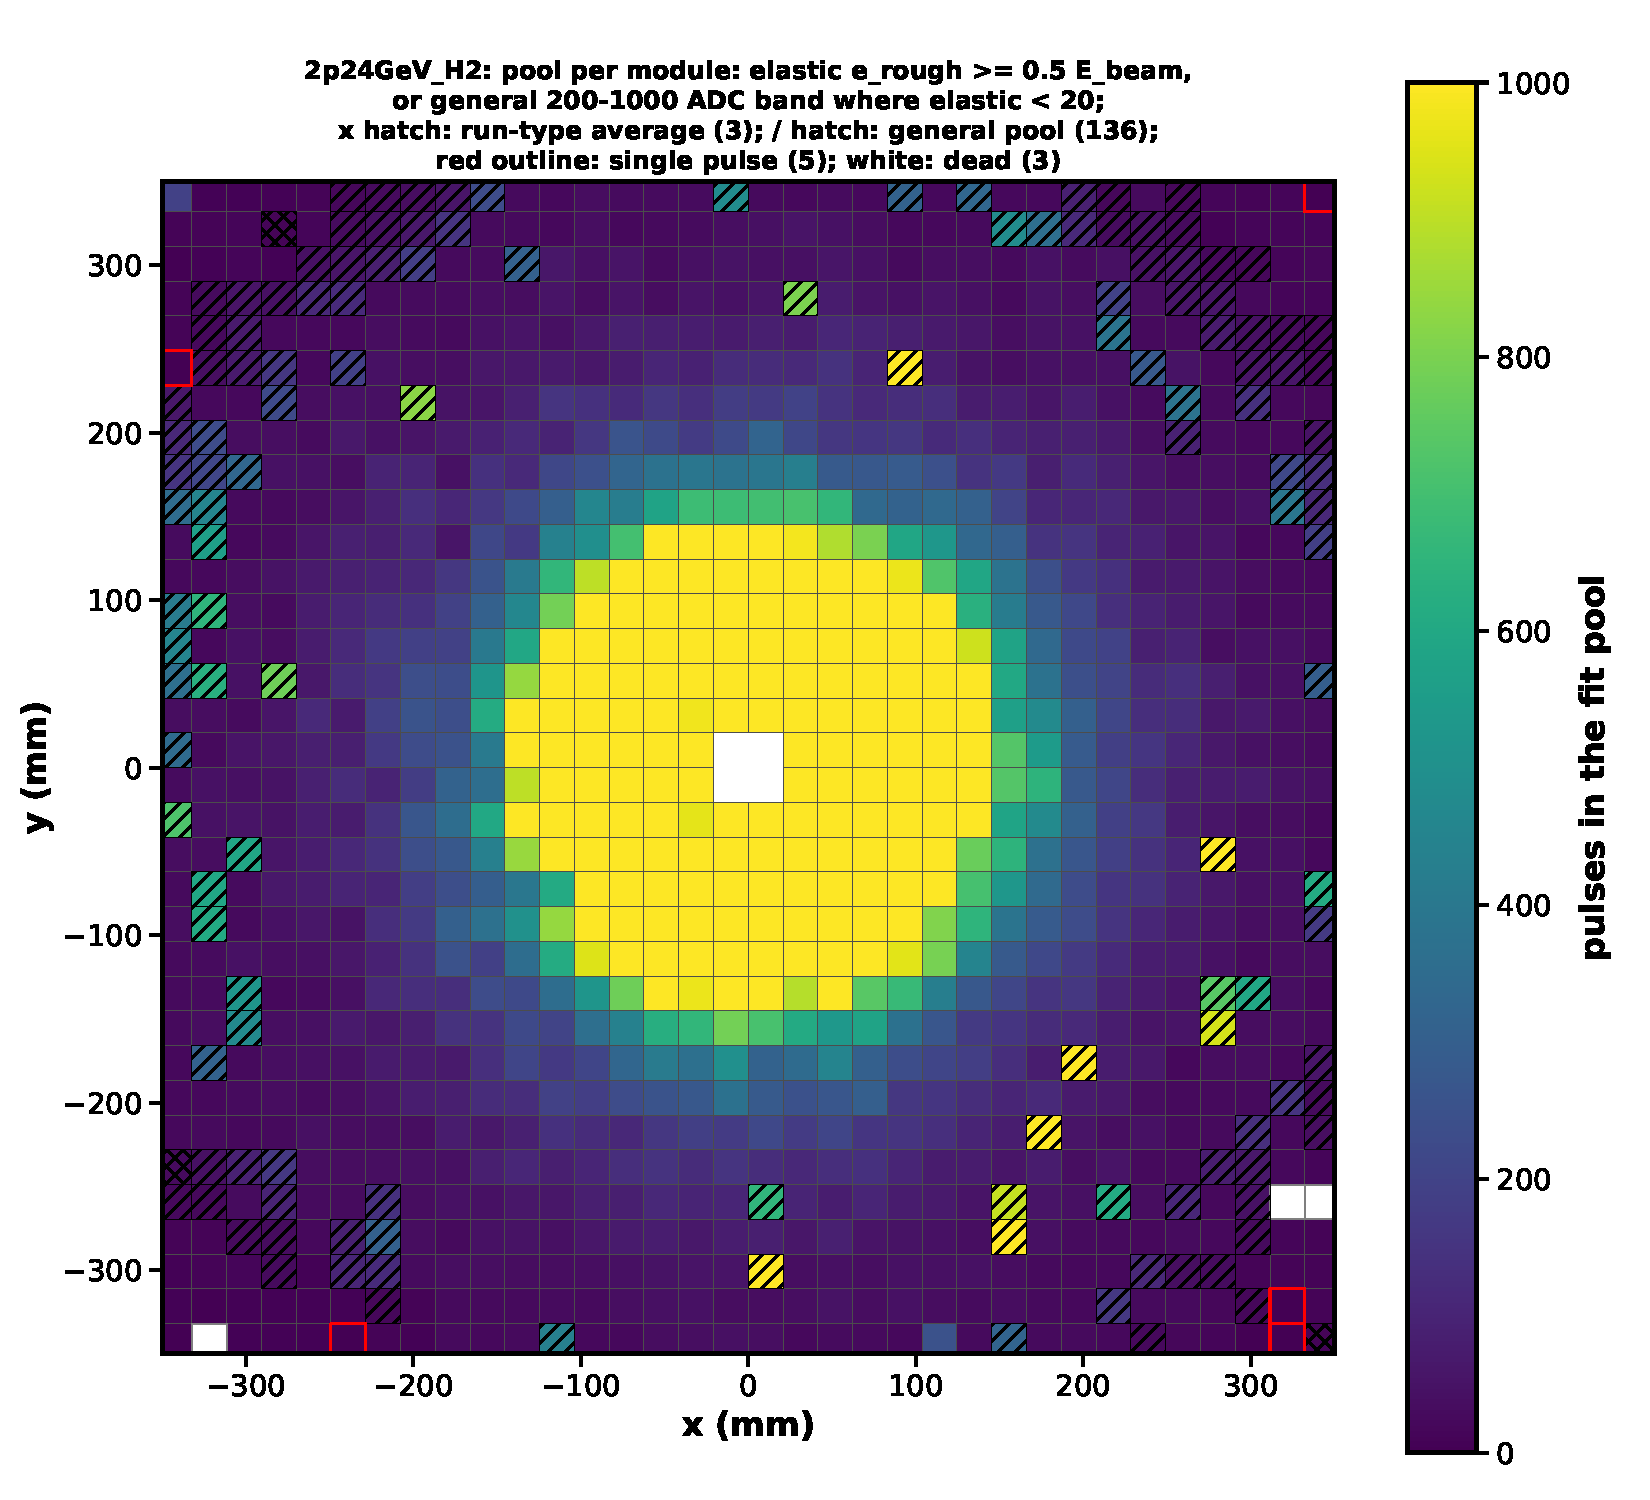
\includegraphics[width=0.85\textwidth]{summary_pool_map.pdf}
\caption{Fit-pool size per module for the \code{2p24GeV\_H2} build. Each rectangle sits at the module's HyCal position ($x$ and $y$ in mm); the colour gives the number of pulses in the fit pool, capped at 1000. Cross hatching marks modules with the run-type average, slash hatching general-pool modules, a red outline single-pulse modules, and white dead modules. The title states the pool rule and the module counts.}
\label{fig:poolmap}
\end{figure}

\subsection{Per-pulse preprocessing}
\label{sec:prep}

Each pooled pulse is baseline-subtracted with its WaveAnalyzer pedestal, $y_{ij} = s_{ij} - p_i$; no pedestal refit and no slope correction are applied. The time axis of the pulse is $\tau_{ij} = t_j - t_{0,i}$, with $t_{0,i} = t^{\mathrm{cfd}}_i$ in the first fit pass and the fitted onset of Section~\ref{sec:align} afterwards. The pulse is normalised to unit amplitude, $\tilde y_{ij} = y_{ij}/A_i$ with point error $\tilde\sigma_i = \sigma_i / A_i$, where $A_i = A^{\mathrm{raw}}_i$ in the first pass and the fitted amplitude afterwards. The peak-sample amplitude of the first pass is biased by the sampling phase; the later passes remove the bias.

Every sample with $\tau_{ij} \ge -20\ns$ (\code{POOL\_TAU\_MIN}) enters the pool of points. Points beyond the data end $T_{\mathrm{data}}$ of Section~\ref{sec:tail} are dropped from the fit.

\subsection{Spline model}
\label{sec:model}

\subsubsection{Basis and knots}

The template is a cubic B-spline on the clamped domain $[-20, 416]\ns$ (\code{T\_LEFT}, \code{T\_AXIS\_END}), with four-fold end knots. The interior knots are non-uniform, dense on the rising edge and sparse in the tail:
\begin{equation}
\{-10,\,-1\} \cup (-1, 10]_{s_0} \cup (10, 20]_{1} \cup (20, 40]_{2} \cup (40, 80]_{4} \cup (80, 160]_{8} \cup (160, 400]_{16},
\end{equation}
where $(a, b]_s$ denotes the knots $a + s, a + 2s, \dots, b$ and $s_0 = 0.5\ns$ for passes with at least 100 kept pulses, else $1\ns$. This gives 79 interior knots (87 knots, 83 coefficients) for the dense plan and 68 interior knots (76 knots, 72 coefficients) otherwise. If the linear solve of Section~\ref{sec:lsq} fails, every spacing is doubled and the fit is repeated, then quadrupled. The knots are placed on the alignment axis of the current pass; the final shift to the onset axis is described in Section~\ref{sec:finalize}.

The fit imposes no constraint: no zero before the onset, no peak or area normalisation. Unit peak and $t = 0$ at the onset are set after the fit (Section~\ref{sec:finalize}). The template is forced to zero for $\tau \le 0$ and $\tau \ge 400\ns$ wherever it is evaluated through the lookup table of Section~\ref{sec:align}: in the alignment and $\chi^2$, and as $f_{\mathrm{ref}}$ in the point variance and the bin detrending. The wiggle check and \code{shape\_sigma} use the raw spline.

\subsubsection{Tail extension}
\label{sec:tail}

With the 0.5\,ns bins of Section~\ref{sec:bins}, $T_{\mathrm{data}}$ is the centre of the last bin holding at least 5 points (\code{TAIL\_BIN\_MIN\_PTS}). An exponential
\begin{equation}
y(\tau) = a\, e^{-(\tau - 140\ns)/\tau_s}
\end{equation}
is fitted by weighted least squares to the bin medians in $[140\ns, T_{\mathrm{data}}]$ (\code{TAIL\_FIT\_FROM}), with bin errors as weights, $a \in [0, 1]$ and $\tau_s \in [20, 2000]\ns$, provided the range holds at least 5 bins. If the range holds fewer than 5 bins or the fit fails, $\tau_s = 170\ns$ (\code{TAIL\_TAU\_DEFAULT}) and $a$ is the median of the bin medians with centre at or above $T_{\mathrm{data}} - 20\ns$, floored at zero, referred to $T_{\mathrm{data}}$. The fitted exponential provides pseudo-points every 4\,ns from $T_{\mathrm{data}} + 4\ns$ to 416\,ns (\code{TAIL\_PSEUDO\_DT}), which keep the spline bounded where the data end.

\subsection{Fit}
\label{sec:fit}

\subsubsection{Point variance}

Each data point $(\tau_{ij}, \tilde y_{ij})$ receives the variance
\begin{equation}
\sigma^2_{ij} = \Big(\frac{\sigma_i}{A_i}\Big)^2 + \big(\sigma_t\, f'_{\mathrm{ref}}(\tau_{ij})\big)^2 + \big(\kappa\, f_{\mathrm{ref}}(\tau_{ij})\big)^2,
\qquad \sigma_t = 0.15\ns,\quad \kappa = 0.012,
\label{eq:var}
\end{equation}
(\code{SIGMA\_T\_NS}, \code{SHAPE\_SIGMA}): the pedestal noise, a timing-jitter term and a relative shape term. $f_{\mathrm{ref}}$ is the unit-peak template of the previous pass ($f_{\mathrm{ref}} \equiv 0$ in the first pass) and $f'_{\mathrm{ref}}$ its central difference over $\pm 0.05\ns$. The weight of a point is $u_{ij} = 1/\sigma_{ij}$. A tail pseudo-point receives the weight $\median_b (1/s_b)$ over all bins, where $s_b$ is the bin-median error of Section~\ref{sec:bins}; this is the weight of a bin median, roughly $\sqrt{n_b}$ times that of a single point.

\subsubsection{Penalised weighted least squares}
\label{sec:lsq}

Let the index $k$ run over data points and pseudo-points, $x_k$ be the time $\tau$ of point $k$, $B_{kl} = B_l(x_k)$ the design matrix of the cubic basis and $W = \operatorname{diag}(u_k^2)$ the weight matrix. The penalty Gram matrix is
\begin{equation}
P_{lm} = \int_{-20}^{416} B''_l(t)\, B''_m(t)\, dt,
\end{equation}
evaluated as a Riemann sum with 0.05\,ns steps. The coefficients minimise
\begin{equation}
\hat c = \argmin_c \sum_k u_k^2 \Big( \tilde y_k - \sum_l c_l B_l(x_k) \Big)^2 + \lambda\, c^{\top} P c .
\end{equation}
The solution follows from the normal equations
\begin{equation}
\big( B^{\top} W B + \lambda P \big)\, \hat c = B^{\top} W \tilde y .
\label{eq:normal}
\end{equation}
The amplitudes and onsets of the pulses are fixed from the previous pass; they are not parameters of this solve. The trigger-synchronous readout places most pulses of a module at one sub-sample phase, so an unpenalised spline would be free to oscillate between the populated phases; the penalty acts where the data leave the shape undetermined.

\subsubsection{Normalisation and onset}
\label{sec:finalize}

On a 0.01\,ns grid over $[-15, 80)\ns$ let $v_{\max}$ be the maximum of the fitted spline $\hat f$. The onset $t_{\mathrm{on}}$ is the last crossing of $0.005\, v_{\max}$ (\code{ONSET\_FRAC}) before the peak, linearly interpolated. The stored template is
\begin{equation}
f(t) = \hat f(t + t_{\mathrm{on}}) / v_{\max},
\end{equation}
implemented as a knot shift $t \to t - t_{\mathrm{on}}$ and a coefficient scale $c \to c / v_{\max}$, so that $f(0) = 0.005$ and $\max f = 1$.

\subsubsection{Bin statistics}
\label{sec:bins}

The pooled points are binned in $\tau$ with 0.5\,ns width (\code{BIN\_W}). Within a bin each point is detrended to the bin centre $\tau_b$ with the reference template, $\tilde y_{ij} - [f_{\mathrm{ref}}(\tau_{ij}) - f_{\mathrm{ref}}(\tau_b)]$. The bin median $m_b$ and its error
\begin{equation}
s_b = \max\Big( \frac{1.4826\, \MAD_b}{\sqrt{n_b}},\ \frac{\sqrt{\bar{\tilde\sigma}_b^2 + (\sigma_t f'_{\mathrm{ref}}(\tau_b))^2}}{\sqrt{n_b}} \Big)
\label{eq:sb}
\end{equation}
are computed from the detrended values, with $n_b$ the number of points, $\MAD_b$ their median absolute deviation and $\bar{\tilde\sigma}_b$ the mean of $\sigma_i/A_i$ in the bin. The bin statistics serve the tail fit, $T_{\mathrm{data}}$ and the shape error of Section~\ref{sec:unc}; they are not the data of the spline fit.

\subsubsection{Per-pulse realignment}
\label{sec:align}

After each pass the template $f$ is tabulated every 0.05\,ns (\code{LUT\_DT}) with linear interpolation, zero outside $(0, 400)\ns$. For each pulse the alignment uses the 52 consecutive samples (\code{\_NCOL}) starting at index $\lfloor (t_{\mathrm{seed}} - 26\ns)/4\ns \rfloor$, clipped to the readout, and among them only the samples with $\tau_{ij} \in [-20, 160]\ns$ (\code{WIN}). At a trial onset $t_0$ the amplitude is the closed-form least-squares value
\begin{equation}
\hat A_i(t_0) = \frac{\sum_j y_{ij}\, f(t_j - t_0)}{\sum_j f(t_j - t_0)^2},
\end{equation}
and the onset maximises
\begin{equation}
\hat t_{0,i} = \argmax_{t_0}\ \sgn(N)\, \frac{N^2}{D},
\qquad N = \sum_j y_{ij}\, f(t_j - t_0),\quad D = \sum_j f(t_j - t_0)^2 .
\label{eq:t0}
\end{equation}
With the model set to zero outside the window, this equals minimising the unweighted $\sum_j (y_{ij} - \hat A_i f)^2$ over the 52 columns. The search is a nested grid around the seed $t_{\mathrm{seed}} = t^{\mathrm{cfd}}_i + \Delta$, where $\Delta$ is the accumulated axis shift of the passes so far: $\pm 4\ns$ in 0.25\,ns steps (\code{ALIGN\_HW}), then $\pm 0.25\ns$ in 0.05\,ns steps, then $\pm 0.05\ns$ in 0.01\,ns steps. At the result,
\begin{equation}
\chi^2_i/\mathrm{dof} = \frac{1}{n_{\mathrm{win}} - 2} \sum_{j \in \mathrm{win}} \frac{\big(y_{ij} - \hat A_i f(\tau_{ij})\big)^2}{\sigma_i^2},
\label{eq:chi2}
\end{equation}
with $n_{\mathrm{win}}$ the number of window samples. A pulse is kept (\code{ok}) when $\hat A_i > 0$, $\chi^2_i$ is finite and $n_{\mathrm{win}} > 10$.

\subsubsection{Iteration}

A template build consists of a fixed number of passes (\code{ALIGN\_PASSES} $= 3$): pool the points, compute the bin statistics, fit the spline, normalise, then realign every pulse to the new template; after three such passes a fourth, final fit closes the build. There are four spline fits and three realignments; no convergence test is applied. The pool of each pass uses the onsets and amplitudes of the preceding realignment and drops the pulses that failed the \code{ok} test. The recorded alignment rms of a pass is the standard deviation over kept pulses of $\hat t_{0,i} - t^{\mathrm{cfd}}_i$; the output stores the value of the last realignment. After the final fit the onsets are moved to the final axis, $\hat t_{0,i} \to \hat t_{0,i} + t_{\mathrm{on}}$, and $\hat A_i$ and $\chi^2_i$ of every pulse are re-evaluated against the final template at that onset without a new search. Figure~\ref{fig:grid_inner} shows the final templates of the innermost-ring modules over their pooled points.

\begin{figure}[htbp]
\centering
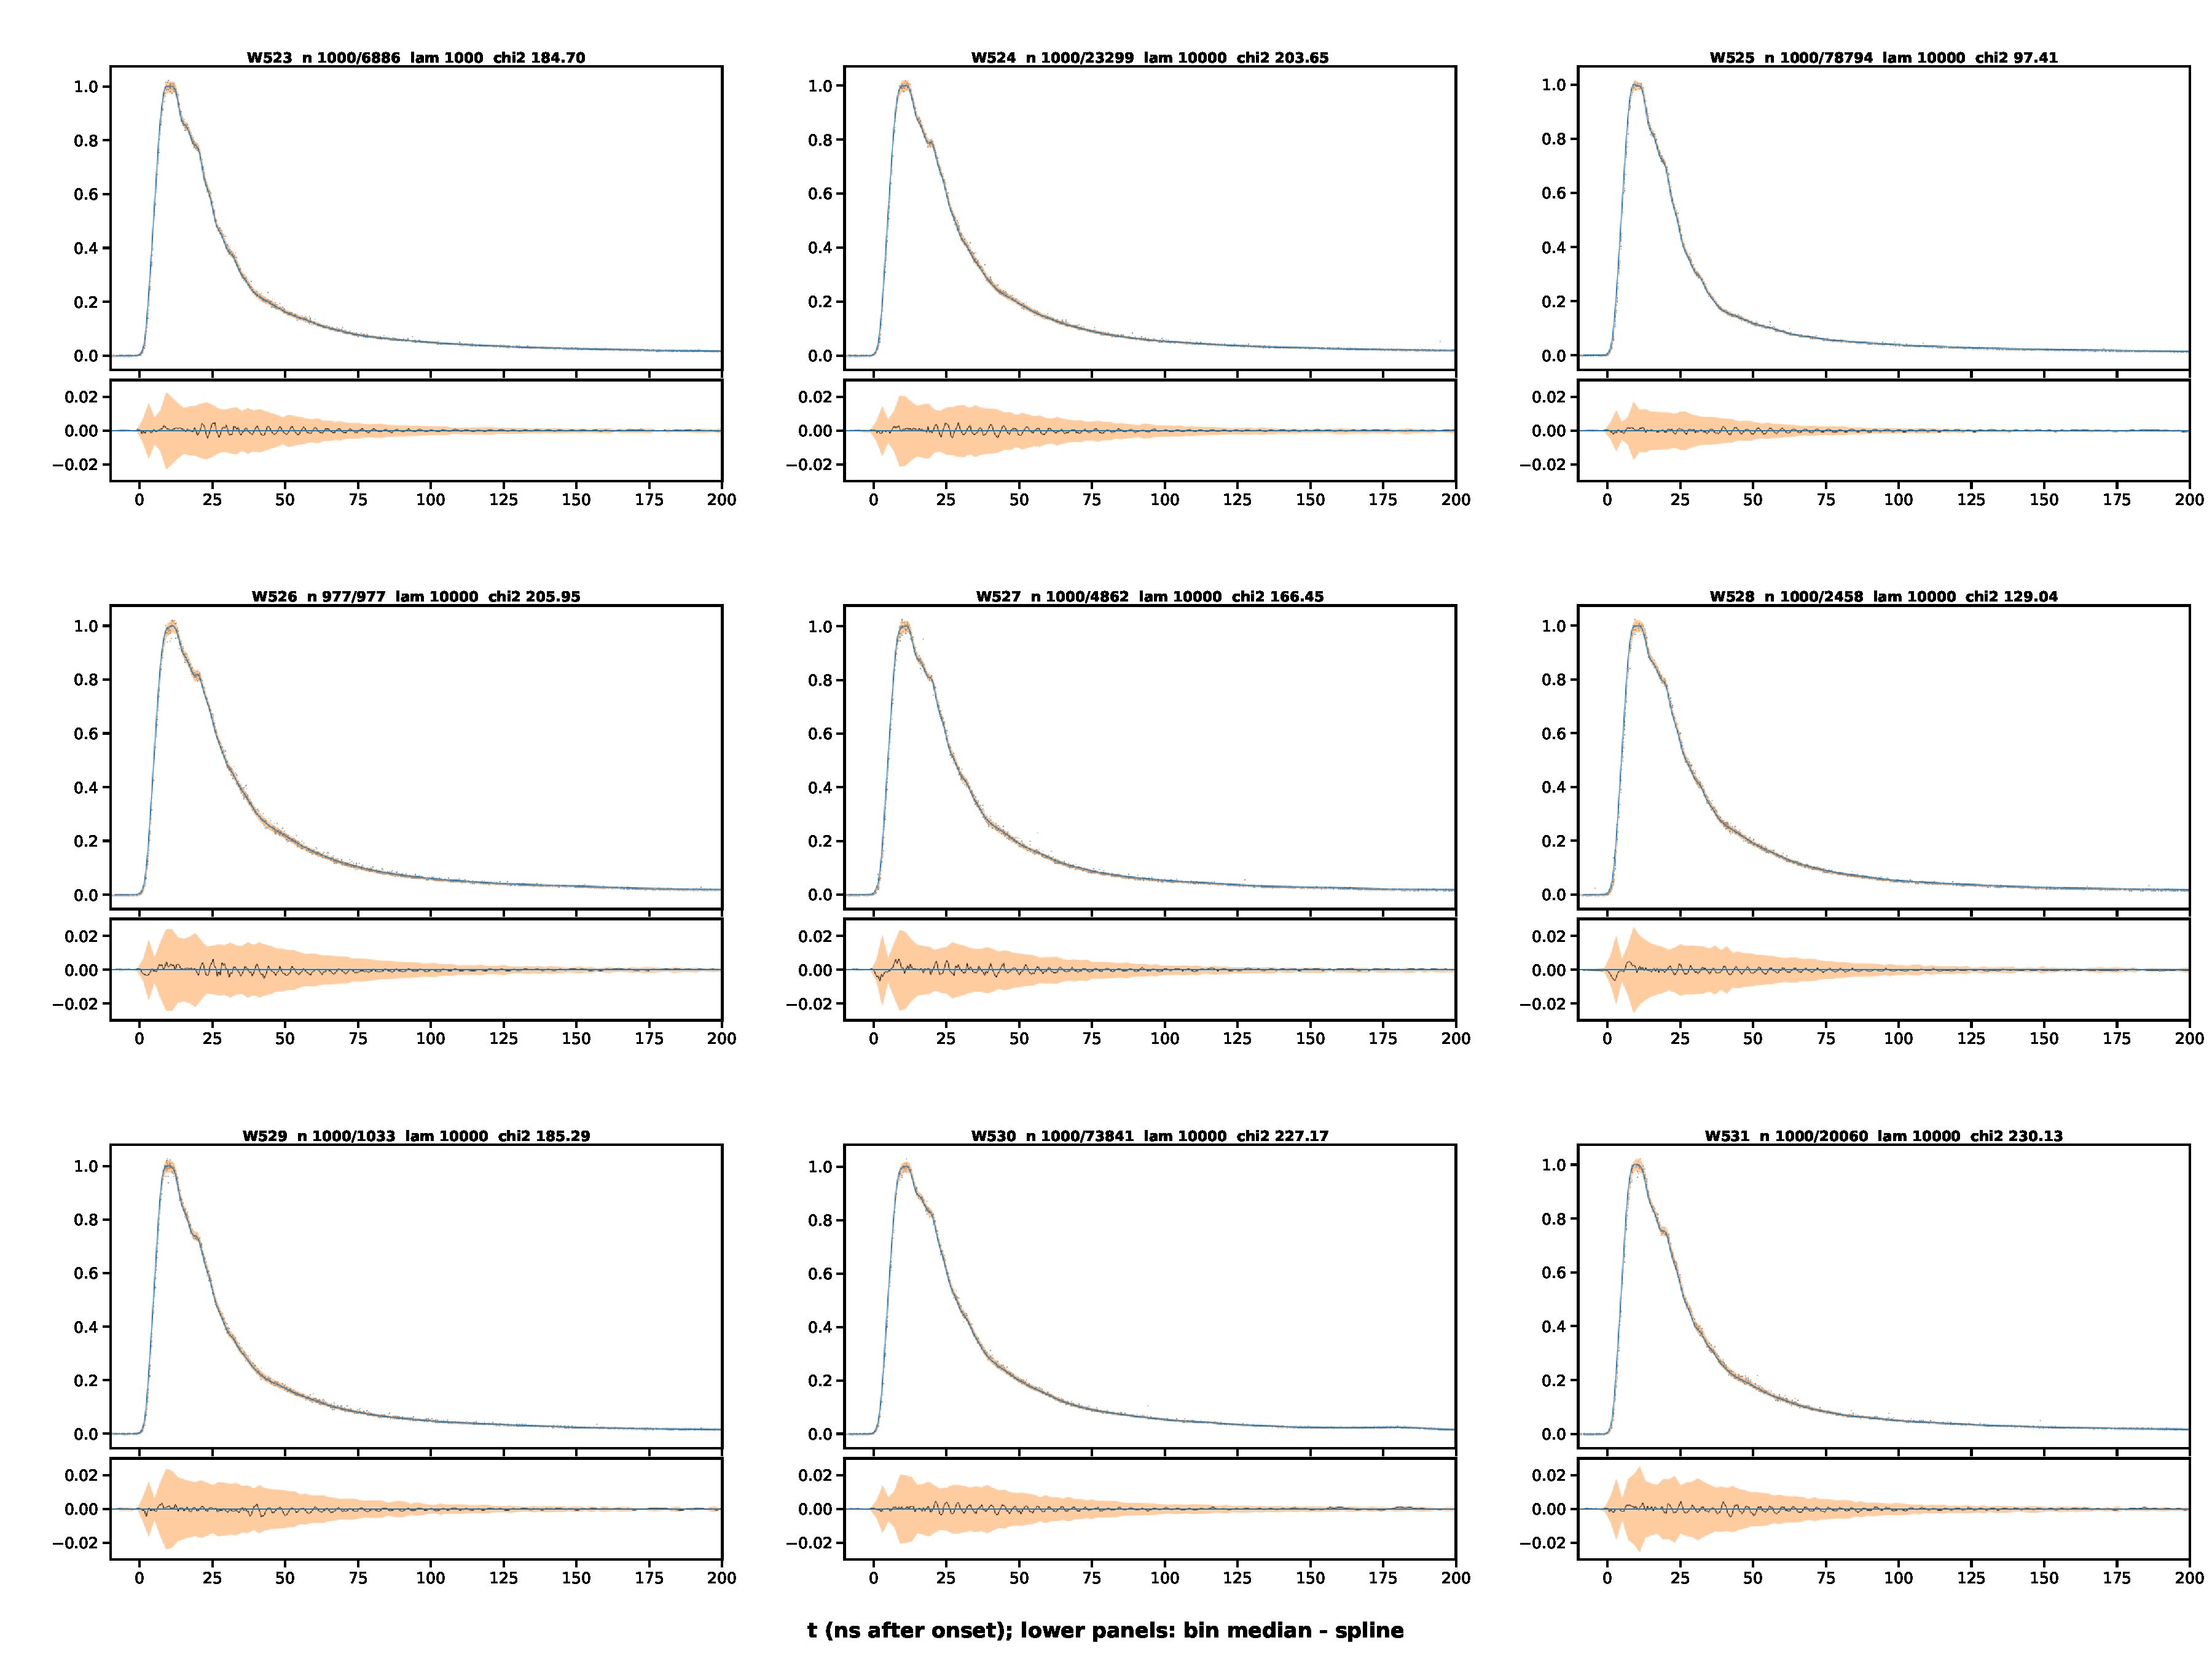
\includegraphics[width=\textwidth]{template_w526_elastic.pdf}
\caption{Templates of the innermost-ring modules W523 to W531 (\code{2p24GeV\_H2}, elastic pools). Upper panel per module: up to 3000 random pooled points $\tilde y_{ij}/v_{\max}$ on the final axis (grey dots), the spline $f$ (blue line) and the band $\pm$\code{shape\_sigma} (orange). Lower panel: bin median minus spline (black line) with the same band, on a $\pm 0.03$ scale. The abscissa is $t$ in ns after the onset, from $-10$ to 200\,ns. Each title gives $n_{\mathrm{pool}}/n_{\mathrm{pool,total}}$, $\lambda$ and the median $\chi^2/\mathrm{dof}$ of Eq.~\eqref{eq:chi2} over the kept pulses.}
\label{fig:grid_inner}
\end{figure}

\subsubsection{Outliers}

The only rejection is the \code{ok} test of Section~\ref{sec:align}. There is no $\chi^2$ cut and no sigma clipping; the spline fit is a plain weighted least squares on all points of the kept pulses, so a bad pulse that passes the test enters at full weight. Medians are used only in the bin statistics and the uncertainty estimators.

\subsubsection{Choice of the smoothing parameter}
\label{sec:lambda}

When the pool holds at least 10 pulses (\code{LAMBDA\_MIN\_POOL}) and a held-out set exists, the template is built for each $\lambda \in \{10^2, 10^3, 10^4\}$ (\code{LAM\_GRID}). The held-out pulses are aligned to each candidate template as in Section~\ref{sec:align}, and the chosen $\lambda$ minimises the mean, over the held-out pulses that are \code{ok} for every candidate that was built, of
\begin{equation}
\chi^2_{\mathrm{full},i}/\mathrm{dof} = \frac{1}{n_{\mathrm{win}} - 2} \sum_{j \in \mathrm{win}}
\frac{\big(y_{ij} - \hat A_i f(\tau_{ij})\big)^2}{\sigma_i^2 + \big(\hat A_i \sigma_t f'(\tau_{ij})\big)^2 + \big(\hat A_i \kappa f(\tau_{ij})\big)^2},
\label{eq:chi2full}
\end{equation}
the $\chi^2$ with the full point variance of Eq.~\eqref{eq:var} in amplitude units. If no held-out pulse is \code{ok} for all candidates, or the pool is smaller than 10 pulses, $\lambda = 10^3$ (\code{LAMBDA\_FALLBACK}).

For pools below 100 pulses (\code{OSC\_POOL\_MAX}) a wiggle check follows. On the 0.1\,ns output grid, the main peak is the largest value in $[3, 30]\ns$; any maximum or minimum of prominence at least $0.002$ of the peak value (\code{OSC\_PROM}) within $[2, 150]\ns$ (\code{OSC\_WIN}) and farther than 3\,ns from the main peak (\code{OSC\_EXCL}) counts as spurious. While any is found, $\lambda$ is multiplied by 10, capped at $10^4$ (\code{SMOOTH\_LAMBDA}), and the template rebuilt. A template still wiggly at $10^4$ counts as a failed fit, and the next pool of Section~\ref{sec:pools} is tried.

\subsection{Shape uncertainty}
\label{sec:unc}

\paragraph{Error of the mean shape.} \code{shape\_err} is $s_b / v_{\max}$ of the final pass, Eq.~\eqref{eq:sb}, interpolated onto the output grid and undefined (NaN) beyond $T_{\mathrm{data}}$. It is the statistical error of the template.

\paragraph{Pulse-to-pulse spread.} \code{shape\_sigma} is computed for every non-dead module, whether its template is its own or the fallback, and always from the amplitude band $200$ to $1000\adc$. Up to 1000 random band pulses are drawn with the generator seeded $(1, m, 1)$, a different draw from the general fit pool, and aligned to the module's final template as in Section~\ref{sec:align}. At least 50 aligned pulses must be \code{ok} (\code{SIGMA\_MIN\_POOL}). For every sample with $-8\ns \le \tau_{ij} \le T_{\mathrm{data}} - t_{\mathrm{on}}$ the residual and its noise variance are
\begin{equation}
R_{ij} = \frac{y_{ij}}{\hat A_i} - f(\tau_{ij}),
\qquad
\nu_{ij} = \frac{v_{\mathrm{ped}}\,(1 + 1/n_{\mathrm{ped}})}{\hat A_i^2},
\end{equation}
where $v_{\mathrm{ped}}$ is the mean over the pool of each pulse's sample variance at $\tau < -20\ns$ (\code{PRE\_ONSET\_NS}) and the factor $1 + 1/n_{\mathrm{ped}}$ adds the pedestal error. Here $f$ is the raw spline, which keeps its small pre-onset values, so the samples with $\tau \in [-8, 0]\ns$ are compared with them. In 2\,ns bins $b$ (\code{SIGMA\_BIN\_NS}) the spread $\sigma_b$ is the value $s \ge 0$ that solves
\begin{equation}
\median_{ij \in b} \frac{\big(R_{ij} - \median_b R\big)^2}{s^2 + \nu_{ij}} = 0.4549,
\label{eq:gsigma}
\end{equation}
the right-hand side being the median of a $\chi^2$ distribution with one degree of freedom (\code{CHI2\_1\_MED}). The equation is solved by 40 bisection steps; bins with fewer than 8 points (\code{SIGMA\_BIN\_MIN}) are NaN, and the bin values are linearly interpolated onto the output grid. With $\nu = 0$ the estimator reduces to $1.4826\,\MAD$; the noise is removed per point inside the median. \code{a\_band}, the median $\hat A_i$ of the band pool, records the amplitude at which the spread was measured.

\paragraph{Borrowed spread.} A module with fewer than 50 usable band pulses, or a dead module, gets \code{sigma\_borrowed} $= 1$ and receives, point by point, the median of \code{shape\_sigma} over all modules with their own value (the whole run type, all pool kinds), and the median of their \code{a\_band}. Figure~\ref{fig:grid_outer} shows outer modules, most of them with a borrowed spread.

\begin{figure}[htbp]
\centering
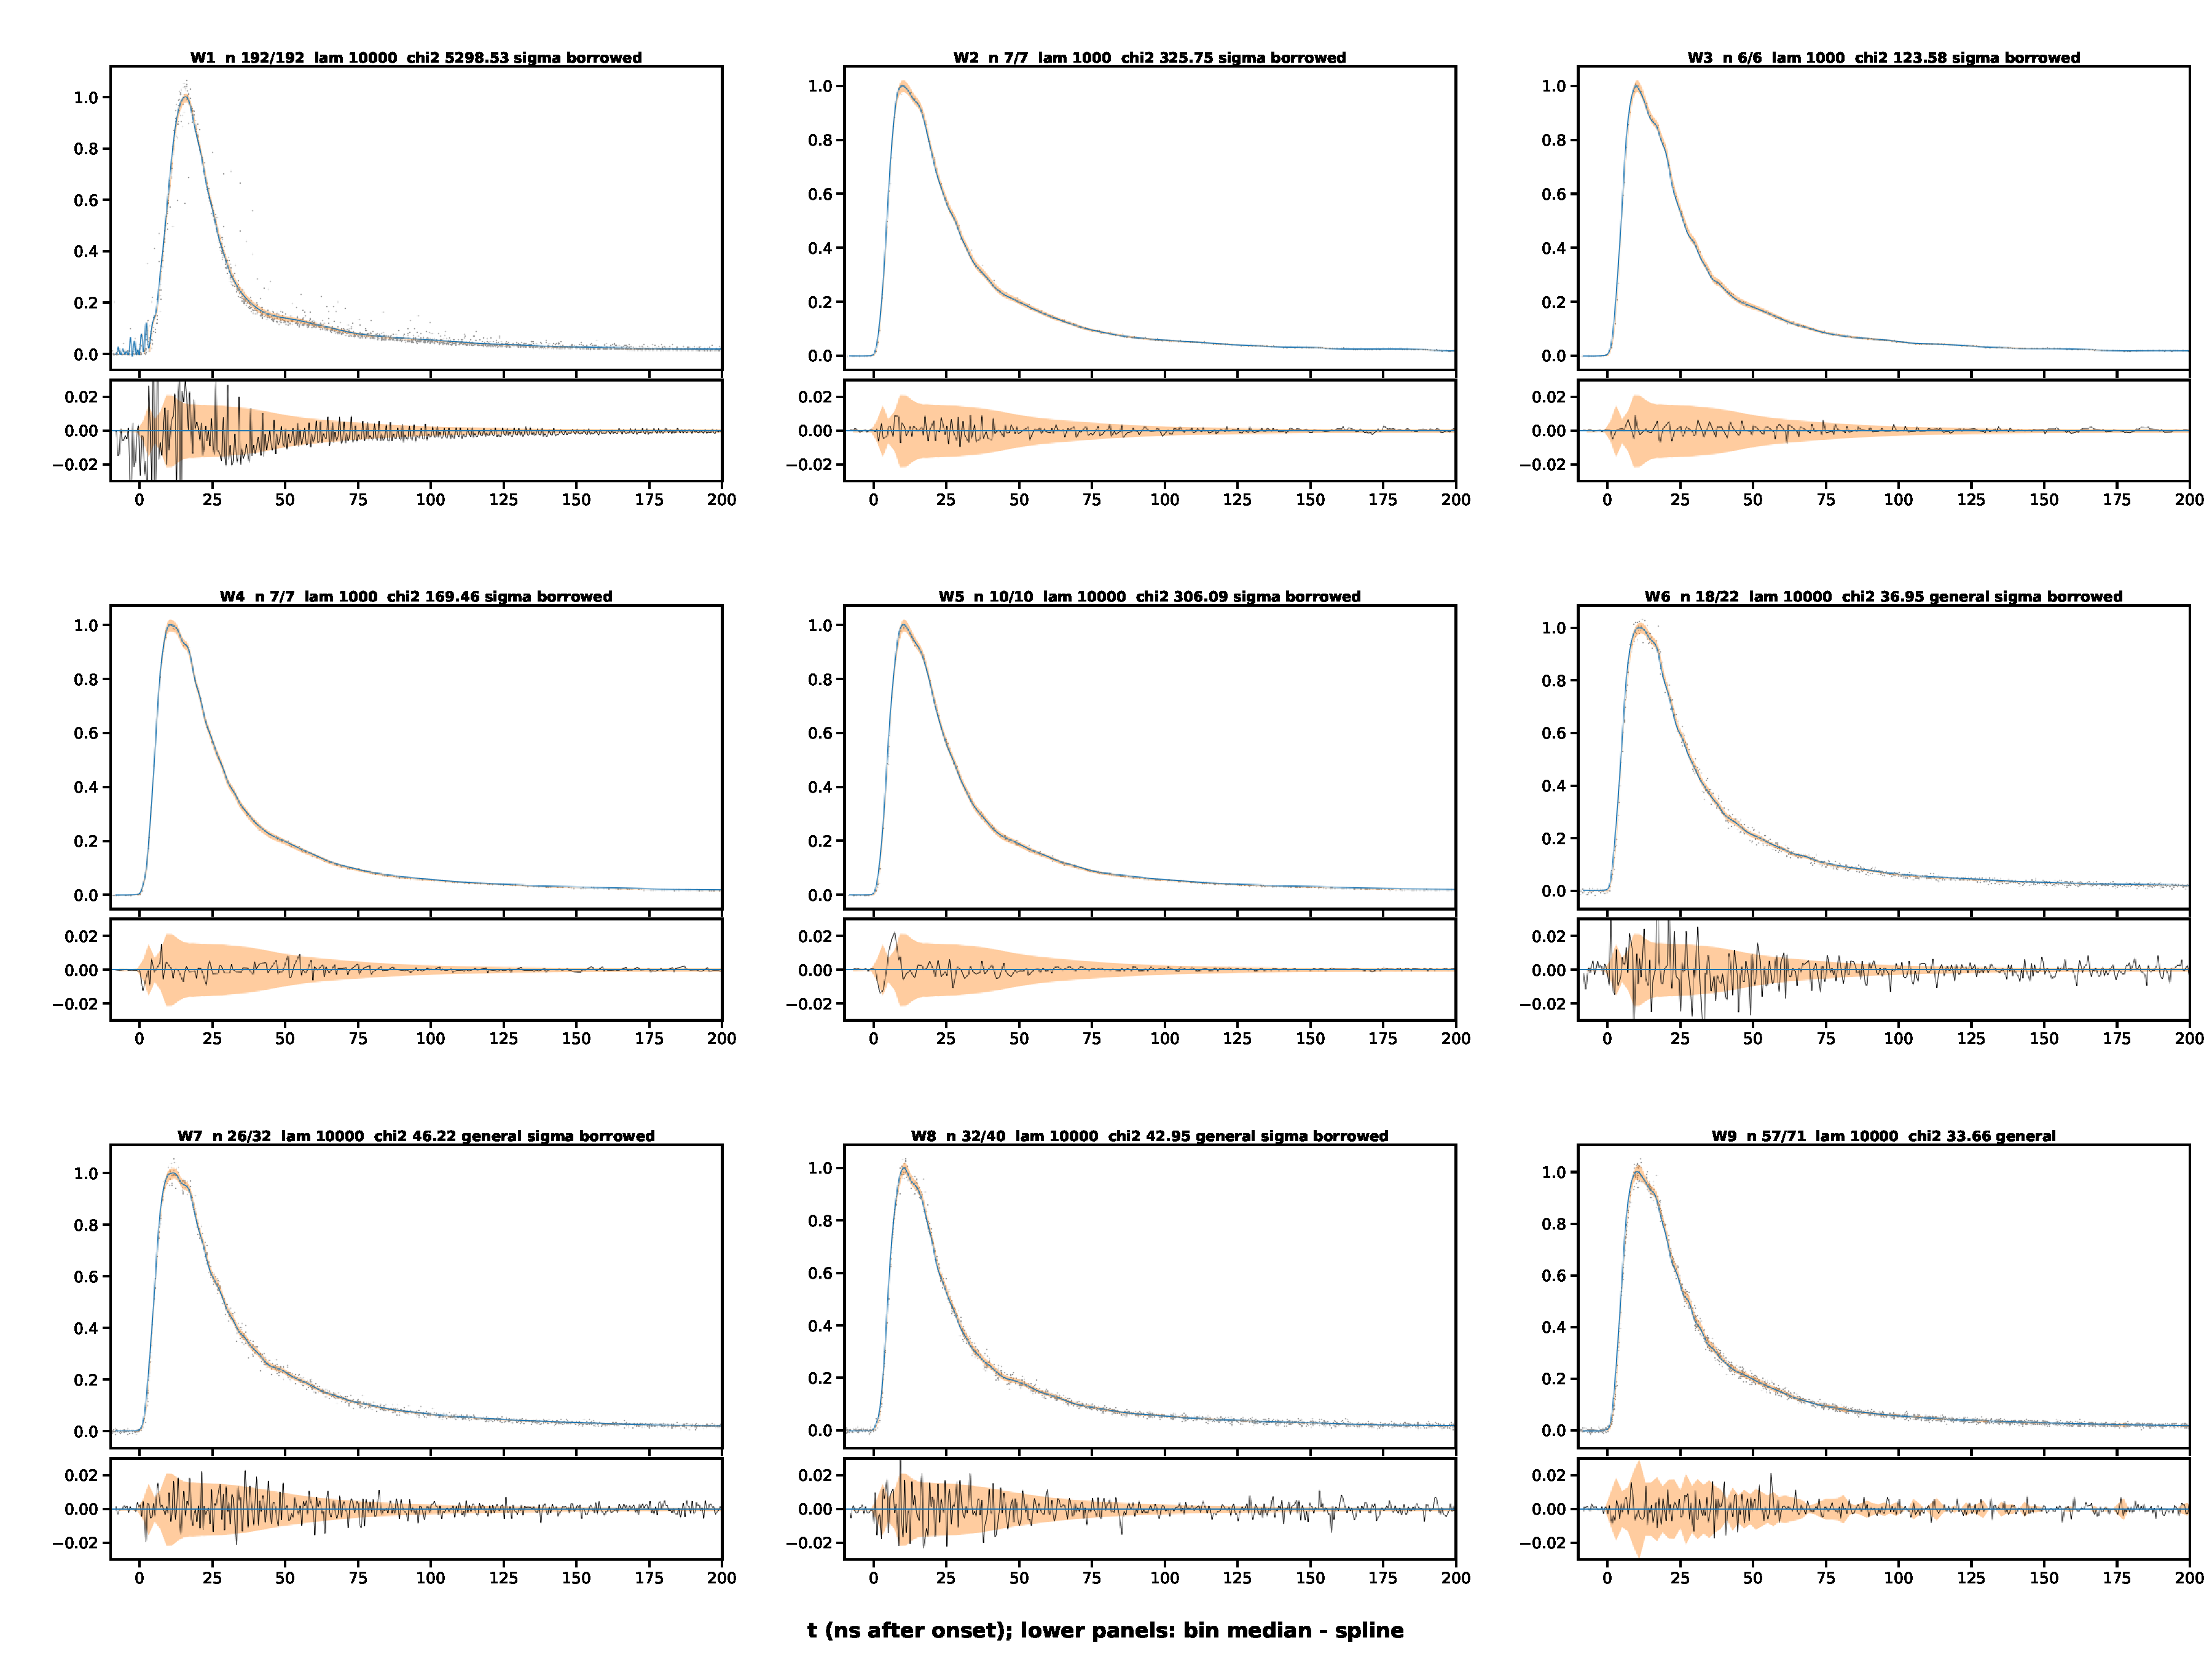
\includegraphics[width=\textwidth]{template_w6_general.pdf}
\caption{As Fig.~\ref{fig:grid_inner} for the outer modules W1 to W9 (\code{2p24GeV\_H2}). W1 to W8 have fewer than 50 usable band pulses and carry the borrowed spread (\code{sigma borrowed} in the title); W1 to W5 were fitted on elastic pools and W6 to W9 on general pools (\code{general}).}
\label{fig:grid_outer}
\end{figure}

\paragraph{Elastic spread.} \code{shape\_sigma\_elastic} applies the same estimator to the elastic fit pool about its own template, only when the template pool is elastic and holds at least 50 pulses; it is NaN otherwise.

\subsection{Fallback and run-type average}
\label{sec:fallback}

A module without its own template receives the run-type average; the \code{fallback} flag of the output takes the values 0 (own template) and 2 (run-type average), with no intermediate level implemented. The run-type average is built with the procedure of Section~\ref{sec:fit} at $\lambda = 10^4$ (\code{SMOOTH\_LAMBDA}) on up to 20 random kept pulses from every module with an own template from an elastic or single pool (the general-pool templates are excluded), drawn with the generator seeded $(1, 987654321)$. It runs the same alignment iteration, with no $\lambda$ scan and no wiggle check. Figure~\ref{fig:grid_avg} shows a module that received the average.

\begin{figure}[htbp]
\centering
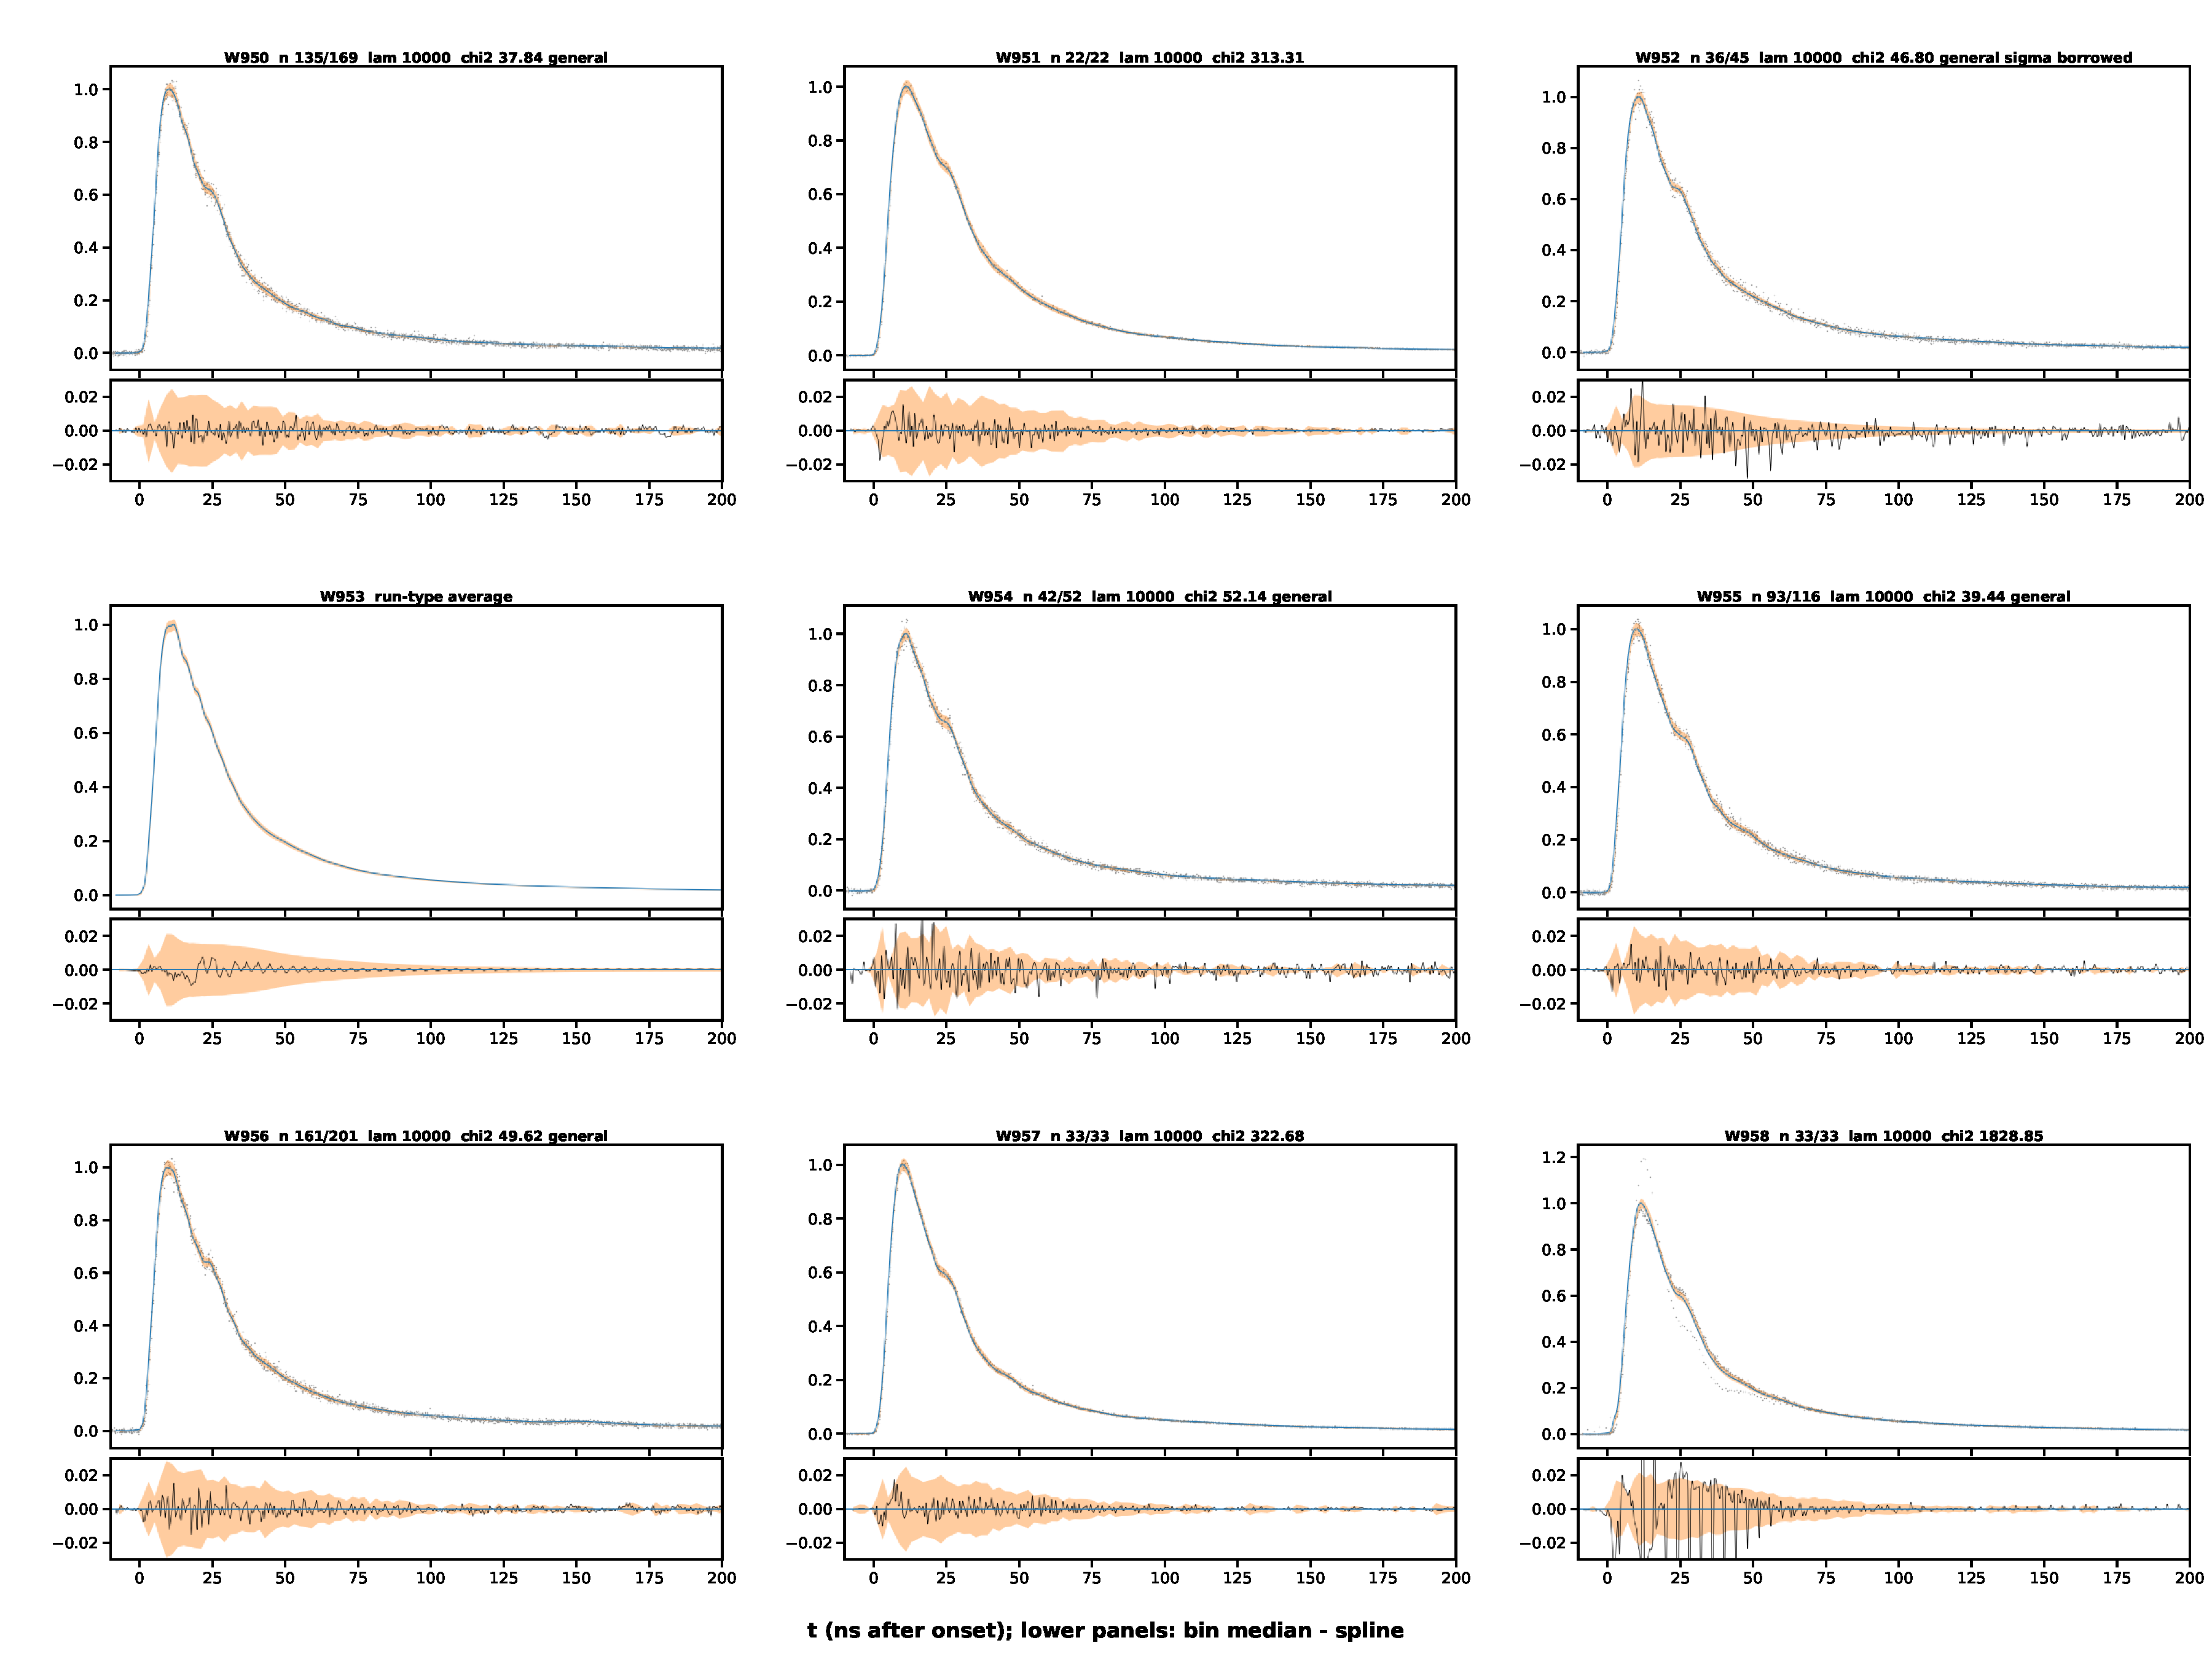
\includegraphics[width=\textwidth]{average_template.pdf}
\caption{As Fig.~\ref{fig:grid_inner} for the modules W950 to W958 (\code{2p24GeV\_H2}). W953 received the run-type average (\code{run-type average} in the title): its panels show the average shape, the borrowed \code{shape\_sigma} band and the residual of the average build, without pooled points. The other modules show their own fits.}
\label{fig:grid_avg}
\end{figure}

\subsection{Outputs and use of the template}
\label{sec:outputs}

The build writes \code{templates\_<RT>.npz} (schema \code{spline\_templates\_v3}), a ROOT file with a per-module tree of the main fields (knots, coefficients, shapes, flags, $\lambda$, \code{chi2\_ndf}, \code{a\_band}), and a PDF of diagnostic pages. Table~\ref{tab:outputs} lists the per-module content. The spline is stored on the final axis, with $t = 0$ at the 0.5\,\% onset and unit peak; the sampled shapes are given on the output grid \code{t\_grid} from $-8$ to 400\,ns in 0.1\,ns steps (\code{GRID\_DT}). In the ROOT file each module also carries a \code{TH1D} of the shape with \code{shape\_sigma} as bin errors.

\begin{table}[htbp]
\centering
\caption{Per-module content of the template file.}
\label{tab:outputs}
\small
\begin{tabular}{p{0.44\textwidth}p{0.50\textwidth}}
\toprule
Field & Content \\
\midrule
\code{spline\_k}, \code{spline\_t}, \code{spline\_c} & degree 3, knots and coefficients, NaN-padded to a common length \\
\code{spline\_nt}, \code{spline\_nc} & true lengths of the knot and coefficient arrays \\
\code{shape}, \code{shape\_err} & template and error of the mean shape on \code{t\_grid} \\
\code{shape\_sigma}, \code{shape\_sigma\_elastic} & pulse-to-pulse spread, band pool and elastic pool \\
\code{a\_band} & median fitted amplitude of the band pool (ADC) \\
\code{onset\_shift\_ns} & final axis minus CFD axis \\
\code{lam\_module} & smoothing parameter used \\
\code{chi2\_ndf} & median of Eq.~\eqref{eq:chi2} over the kept pulses \\
\code{align\_rms\_ns} & alignment rms of the last realignment \\
\code{n\_pool}, \code{n\_pool\_total} & pool size used; candidate count before the cap (elastic) or band size (general) \\
\code{dead}, \code{fallback}, \code{single}, \code{pool\_general}, \code{sigma\_borrowed} & flags \\
\code{t\_pk}, \code{t50} & peak time and half-maximum time of the template (ns) \\
\code{avg\_spline\_t}, \code{avg\_spline\_c} & run-type average spline (one per file) \\
\code{meta} & build record (constants, inputs, git revision) \\
\bottomrule
\end{tabular}
\end{table}

Each one-pulse overlay of the diagnostic pages draws $\hat A_i\, f(t - \hat t_{0,i})$ for $t > \hat t_{0,i}$ over the raw $y_{ij}$, using the final onset and amplitude of the pulse. A single-pulse fit with the template has two free parameters, $t_0$ and $A$, determined by the unweighted least squares of Eqs.~\eqref{eq:t0} and following over $\tau \in [-20, 160]\ns$, with the shape fixed. Figures~\ref{fig:ex_inner} and \ref{fig:ex_outer} show such overlays for an innermost-ring and an outer module.

\begin{figure}[htbp]
\centering
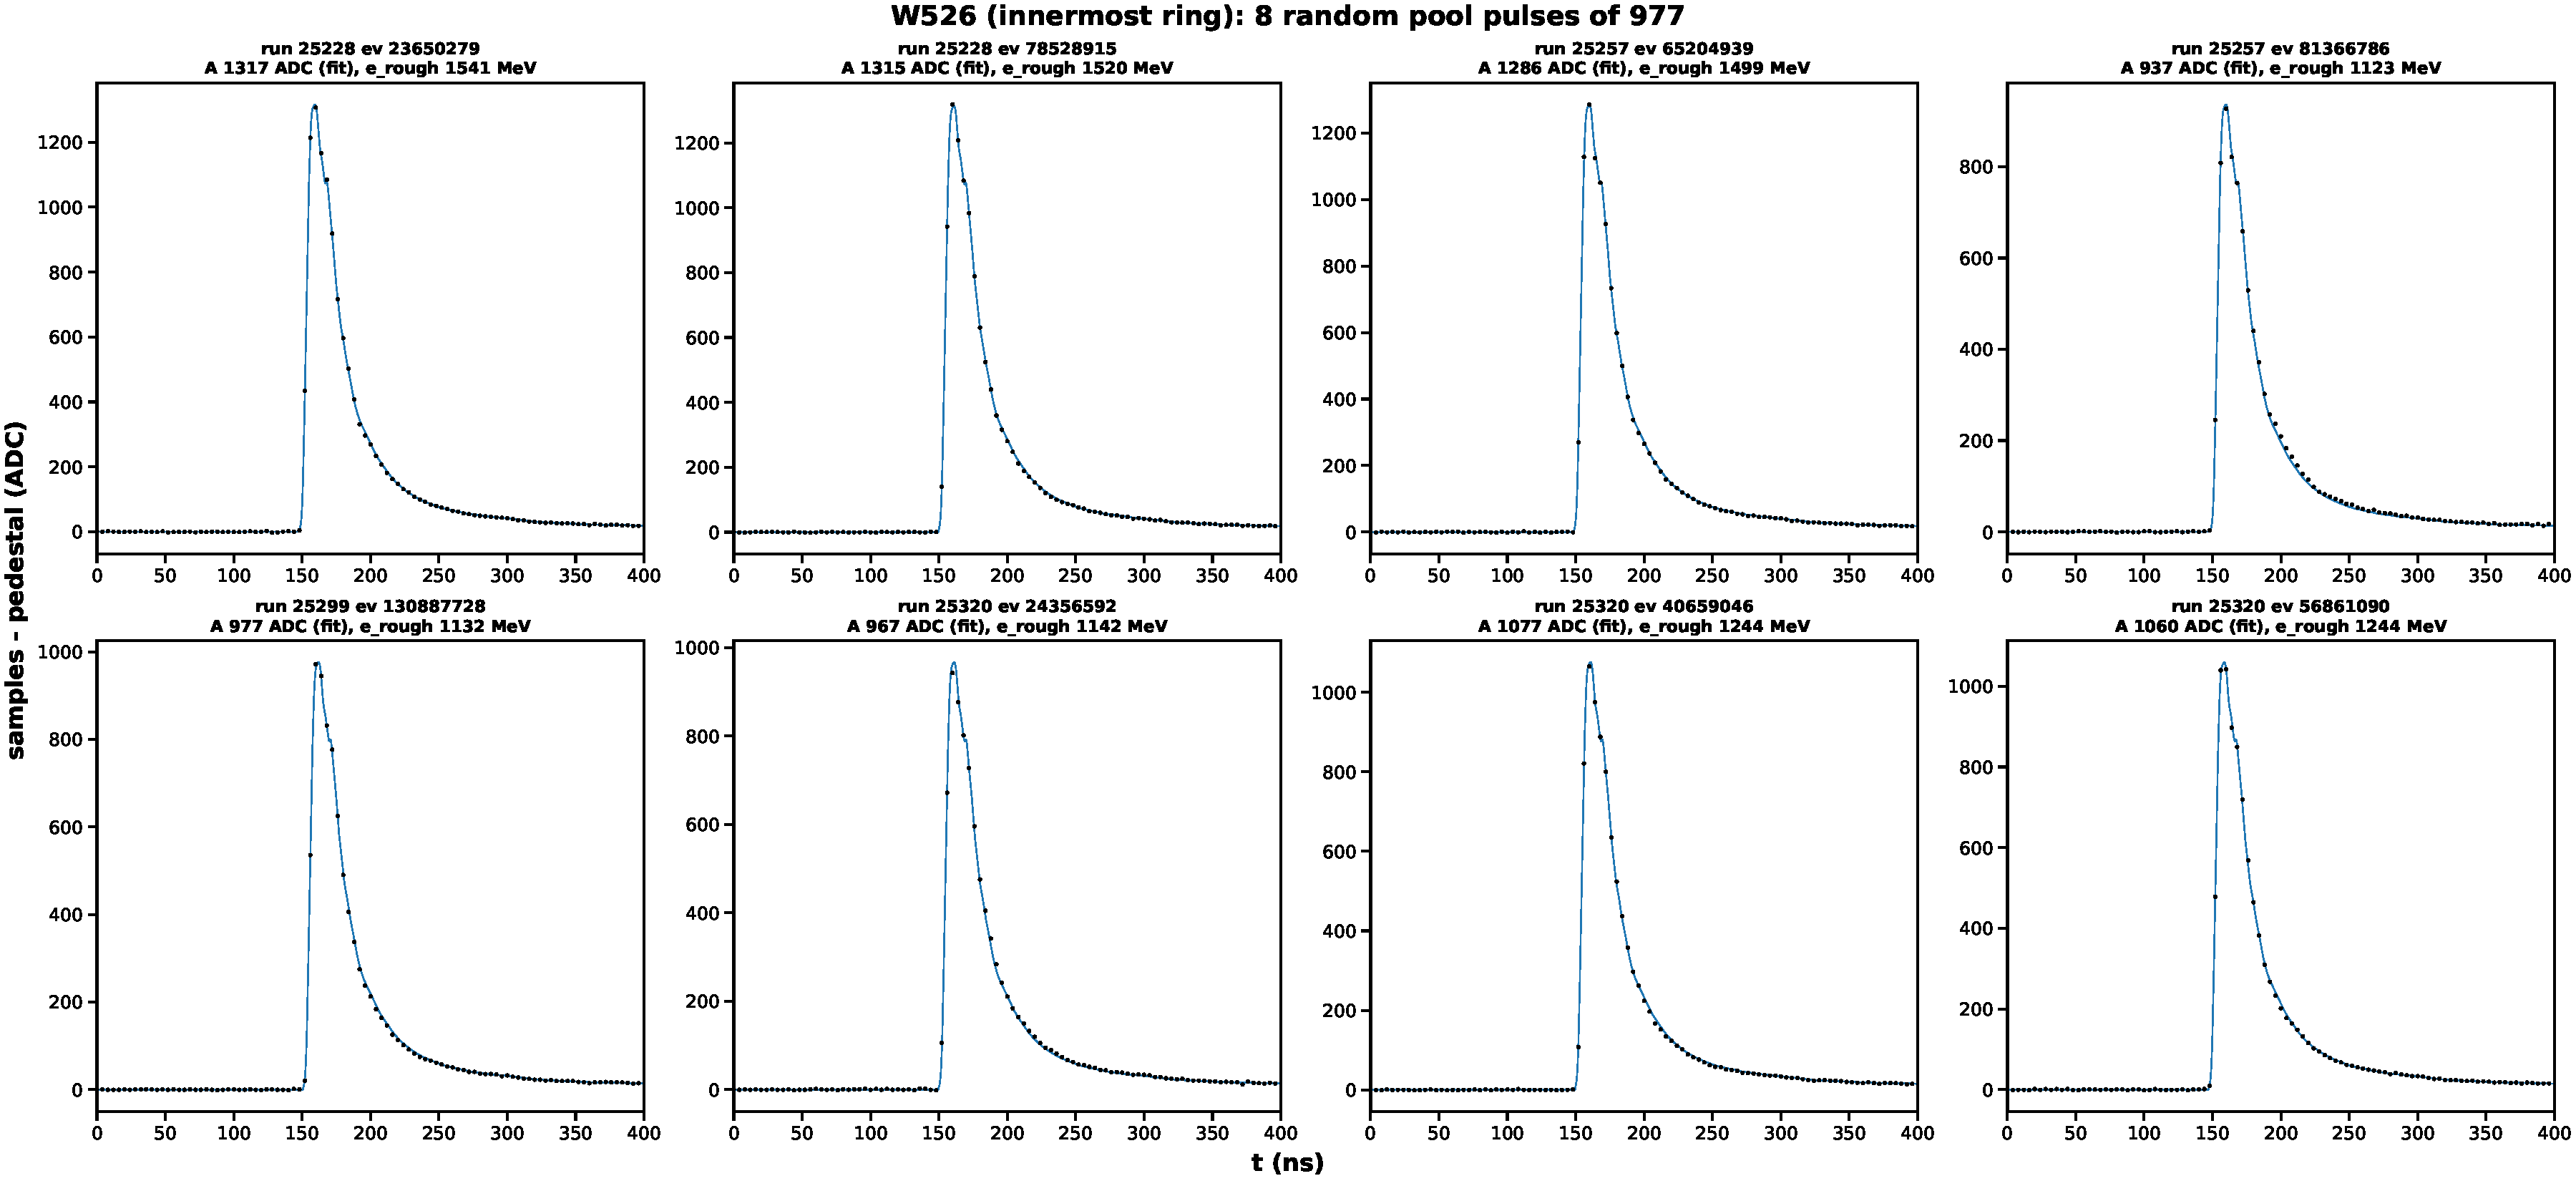
\includegraphics[width=\textwidth]{example_w526_innermost.pdf}
\caption{Eight random pool pulses of W526 (innermost ring, 977 pool pulses, \code{2p24GeV\_H2}). Black dots: pedestal-subtracted samples (ADC) at the 4\,ns sample times; blue line: $\hat A_i\, f(t - \hat t_{0,i})$ on a 0.5\,ns grid, zero for $t \le \hat t_{0,i}$, with the final onset and amplitude of the build. Each title gives the run and event number, the fitted amplitude and $e^{\mathrm{rough}}$.}
\label{fig:ex_inner}
\end{figure}

\begin{figure}[htbp]
\centering
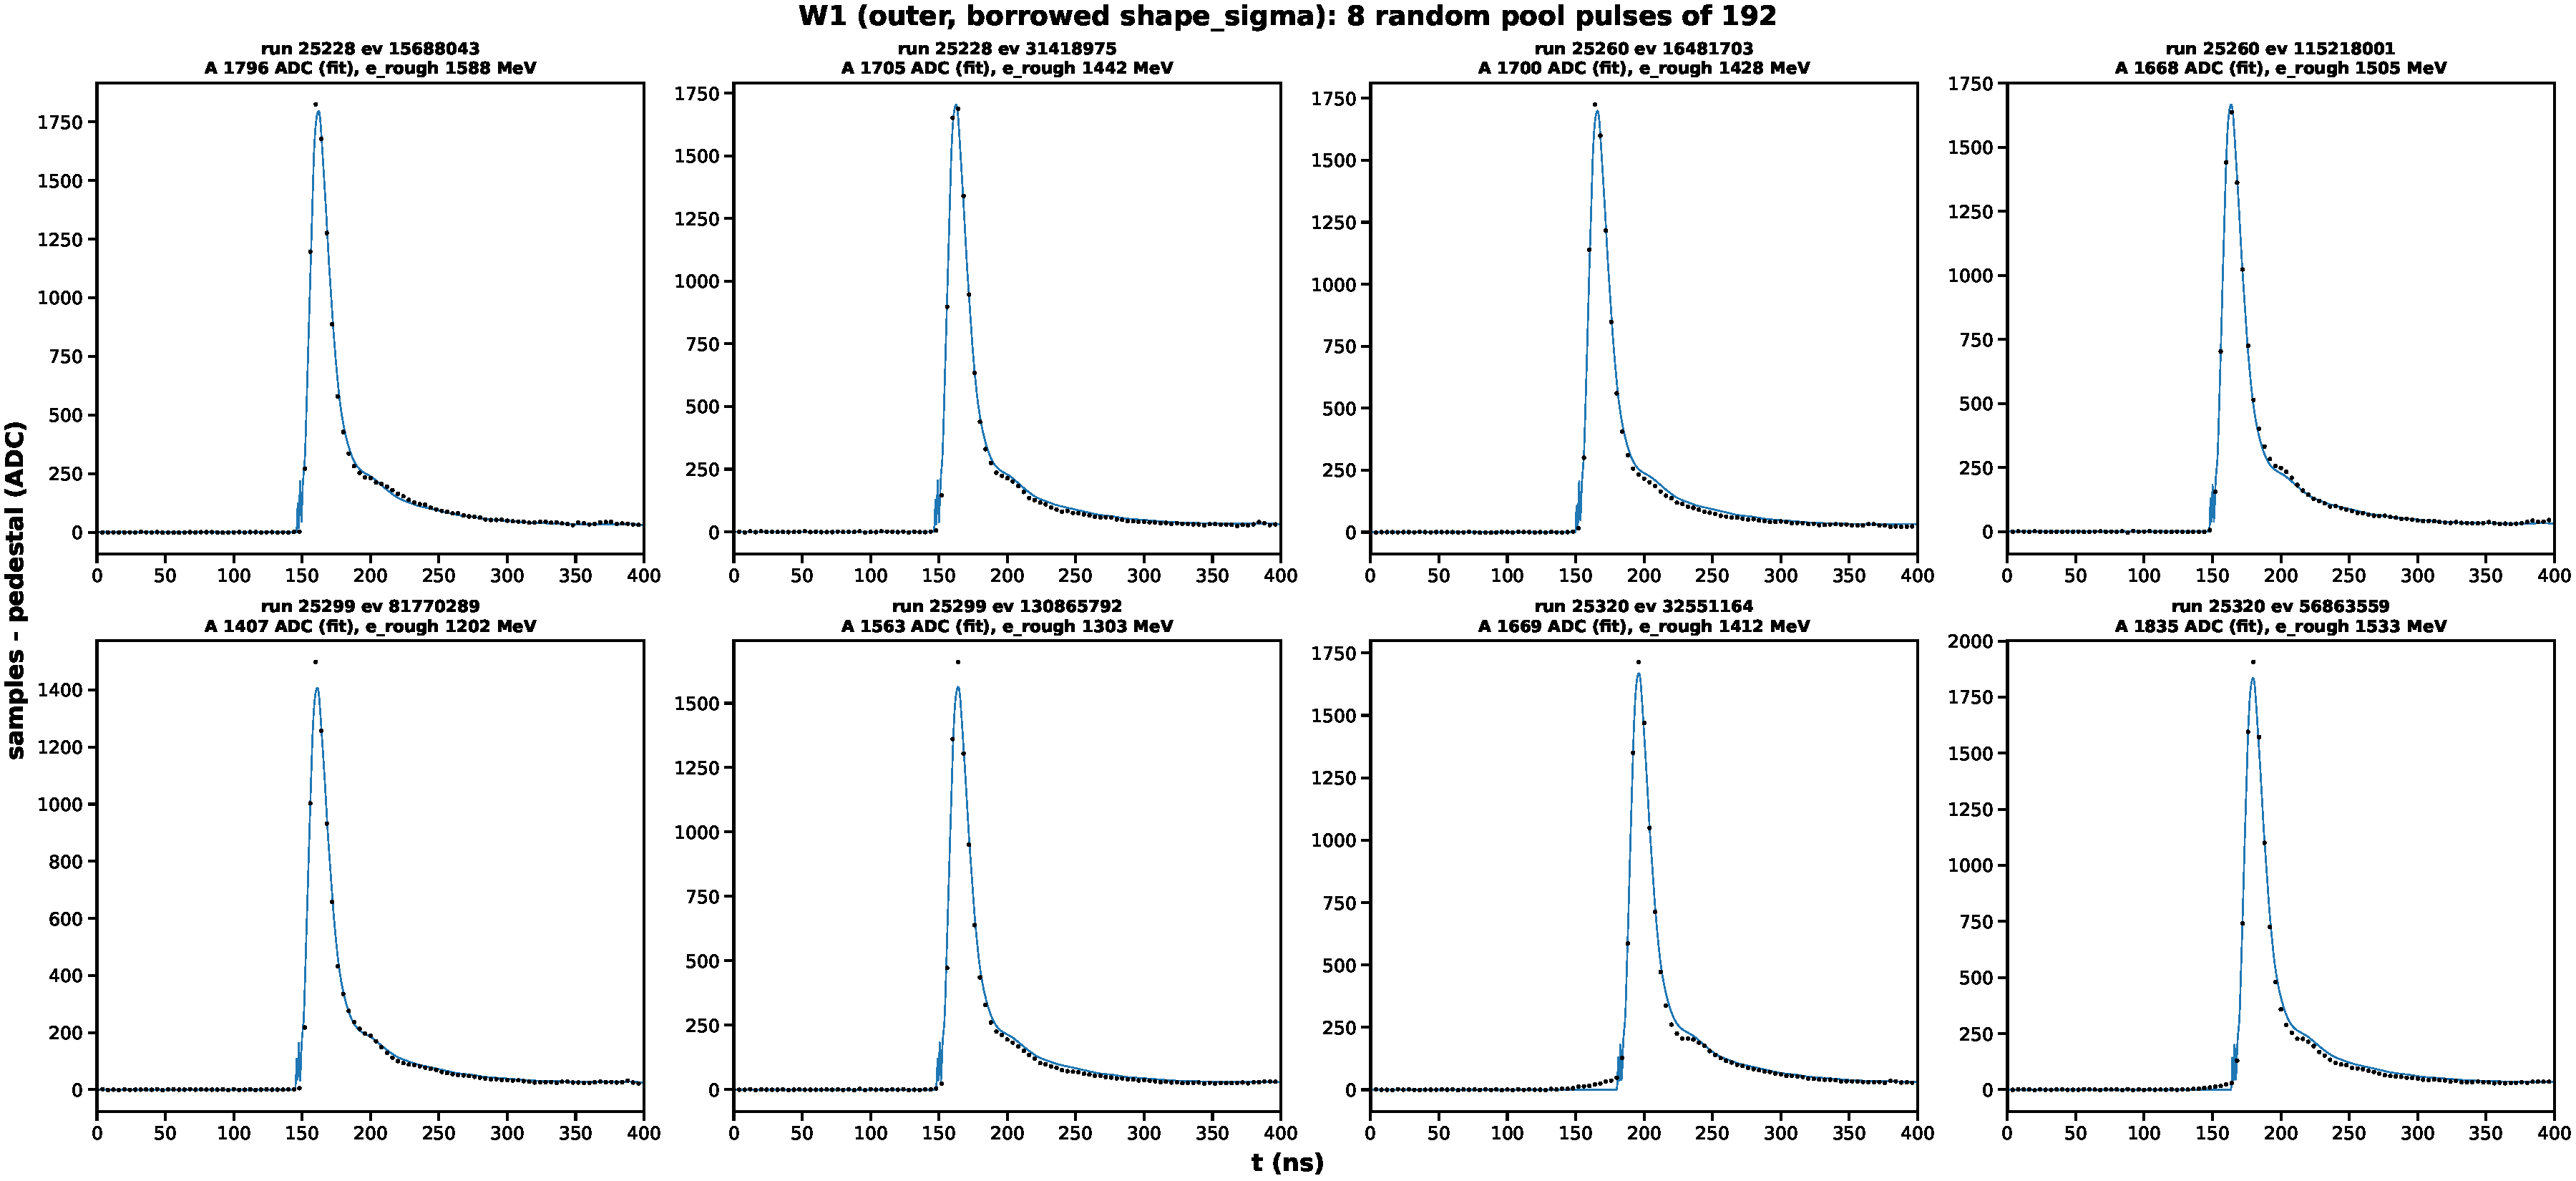
\includegraphics[width=\textwidth]{example_w1_borrowed.pdf}
\caption{As Fig.~\ref{fig:ex_inner} for W1 (outer module with a borrowed spread, 192 pool pulses).}
\label{fig:ex_outer}
\end{figure}

\subsection{Example build}
\label{sec:build}

For the run type \code{2p24GeV\_H2} (numbers from the build log and the npz of that build): 1146 modules received their own template (136 from a general pool, 5 from a single pulse) and 6 the run-type average, 3 of them dead. The median pool size was 86 and 148 modules reached the 1000-pulse cap; 544 modules used the 87-knot plan and 602 the 76-knot plan. The chosen $\lambda$ was $10^2$ for 184 modules, $10^3$ for 148 and $10^4$ for 814. The median alignment rms per pass was 0.101, 0.108 and 0.115\,ns. The run-type average used 19\,502 pulses, and 98 own-template modules borrowed their \code{shape\_sigma}. Figure~\ref{fig:summary} is the summary page of that build.

\begin{figure}[htbp]
\centering
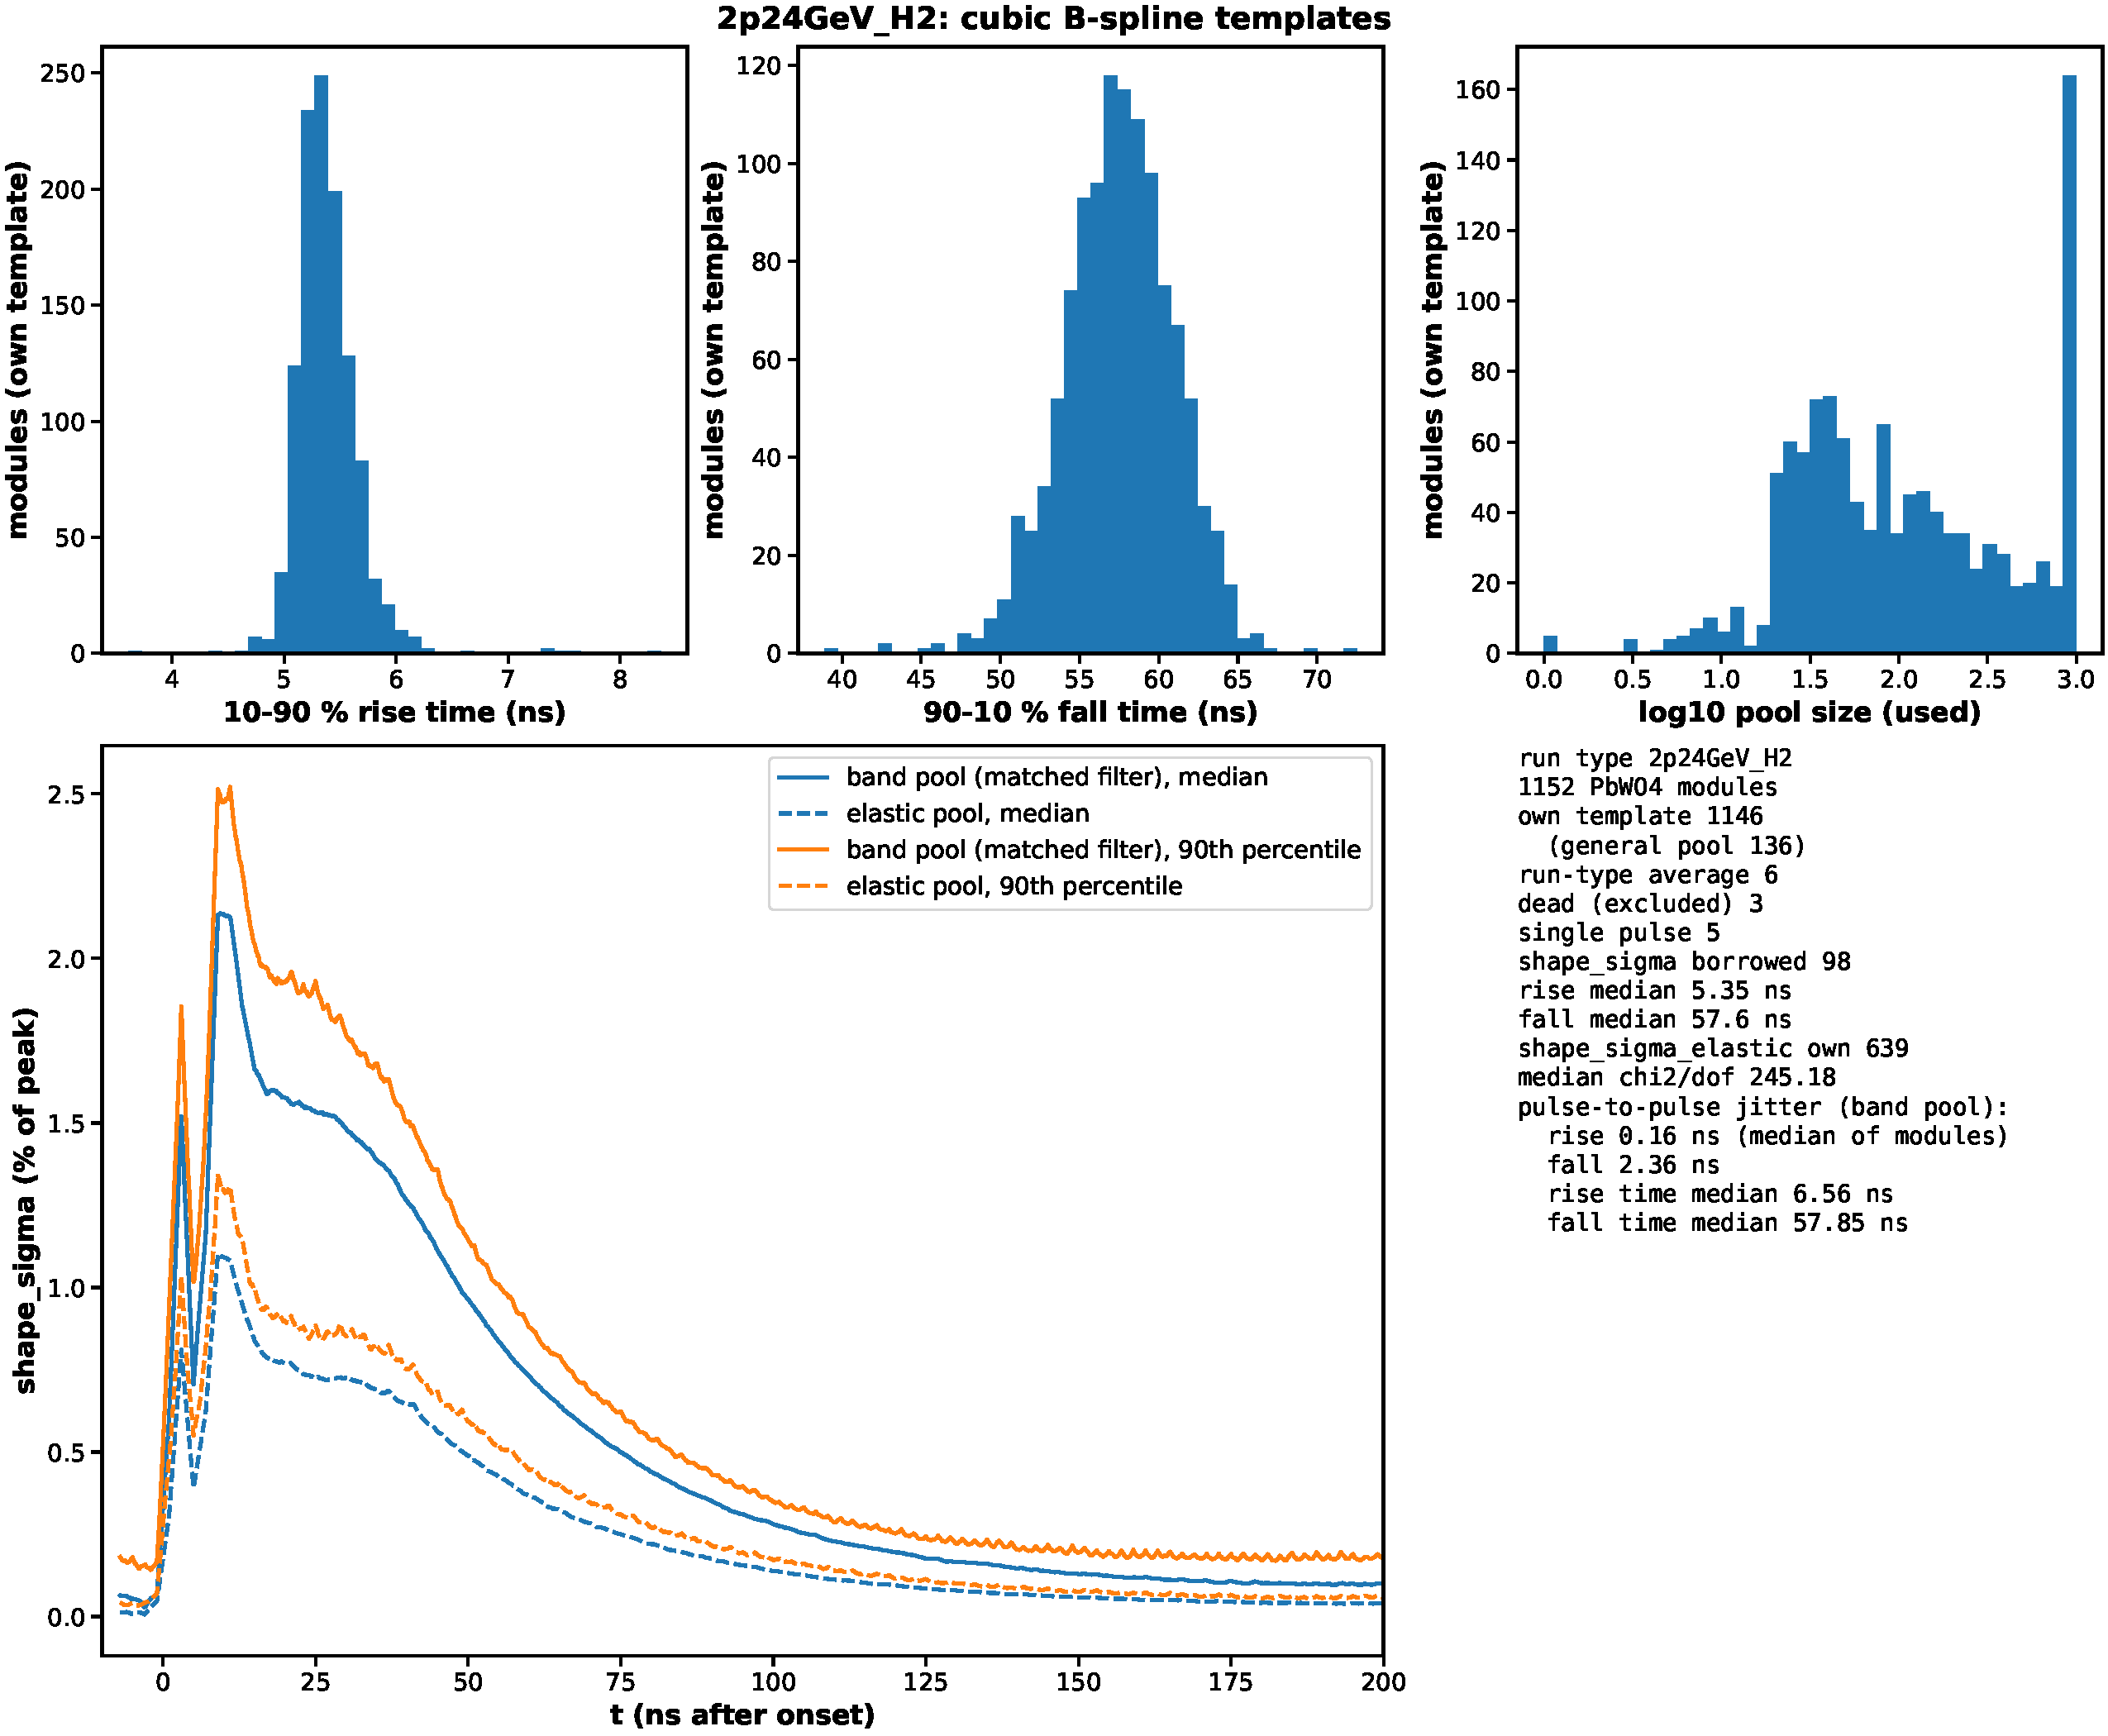
\includegraphics[width=\textwidth]{summary_overview.pdf}
\caption{Summary page of the \code{2p24GeV\_H2} build. Top row: histograms over the own-template modules of the 10--90\,\% rise time and the 90--10\,\% fall time of the template and of $\log_{10}$ of the pool size. Bottom left: \code{shape\_sigma} in percent of the peak versus $t$ for the modules with their own value, the band pool as solid lines and the elastic pool dashed; blue is the median over modules and orange the 90th percentile. Bottom right: module counts and medians of the build.}
\label{fig:summary}
\end{figure}

\section{Pile-up}
\label{sec:pileup}

Two particles that hit one module within the 400\,ns readout give overlapping pulses, and an amplitude read from a single-pulse fit is then biased. This section has four parts. Section~\ref{sec:fitter} describes the multi-pulse template fitter. Section~\ref{sec:rates} applies it to data and counts second pulses per run type and per module. Section~\ref{sec:generator} generates one- and two-pulse waveforms with known truth, and Section~\ref{sec:deconv} measures the fitter on them.

\subsection{Multi-pulse template fitter}
\label{sec:fitter}

\paragraph{Purpose, inputs, outputs.} The fitter decomposes one waveform into up to six template pulses on a constant baseline. Its inputs are the 100 samples of a channel and the bank row of its module (Table~\ref{tab:outputs}): the spline $f$, \code{shape\_sigma}, \code{a\_band} and \code{t\_pk}. Its outputs are the fitted pedestal, the noise, and the onset, amplitude and validity flag of each pulse. The fitter is the class \code{MF} of \code{pileup\_deconvolution\_study.py}; \code{pileup\_rates.py}, \code{crosstalk\_study.py} and \code{energy\_resolution\_benchmark.py} carry identical copies. Table~\ref{tab:mfconst} in Appendix~\ref{app:const} lists its constants. The module \code{mf\_pulse.py} holds an older, sequential fitter with other constants; none of the four scripts imports it.

\subsubsection{Procedure}

\begin{enumerate}
\item \textbf{Template tables.} The spline $f$ of the module is tabulated every 0.05\,ns (\code{LUT\_DT}) and interpolated linearly, with $f = 0$ for $\tau \le 0$ and $\tau \ge 400\ns$. The peak time $t_{\mathrm{pk}}$ is the time of the table maximum. The shape scatter $\sigma_s(\tau)$ is \code{shape\_sigma} on the same grid, floored at 0.005 (\code{SHAPE\_SIGMA\_MIN}) inside $(0, 400)\ns$ and zero outside; $a_{\mathrm{band}}$ is the amplitude at which it was measured (Section~\ref{sec:unc}).
\item \textbf{Baseline, noise and weights.} The noise is $\sigma = \max(1.4826\,\MAD, 0.3\adc)$ of the first 30 samples (\code{PED\_NSAMPLES}, \code{SIGMA\_MIN}). The baseline estimate $\bar p$ is the mean of those of the 30 samples that lie within $\max(2\sigma, 1\adc)$ of their median, and $y_j = s_j - \bar p$. A clipped sample receives the weight $\omega_j = 0$, every other sample $\omega_j = 1$. A waveform is fitted only when its largest three-sample running mean exceeds the noise,
\begin{equation}
\max_j \tfrac{1}{3}\,(y_j + y_{j+1} + y_{j+2}) > \max(3\sigma,\ 3\adc)
\end{equation}
(\code{CAND\_NSIGMA}).
\item \textbf{Matched filter.} For a trial onset $t_0$ the template is correlated with the waveform over the kernel $\mathrm{ker}(t_0)$, the 24 consecutive samples (\code{L}, 96\,ns) that start at the first sample at or after $t_0$:
\begin{equation}
N(t_0) = \sum_{j \in \mathrm{ker}(t_0)} \omega_j\, y_j\, f(t_j - t_0),
\qquad
D(t_0) = \sum_{j \in \mathrm{ker}(t_0)} \omega_j\, f(t_j - t_0)^2 ,
\label{eq:mf}
\end{equation}
\begin{equation}
\hat A(t_0) = \frac{N}{D}, \qquad S(t_0) = \frac{N}{\sqrt{D}}, \qquad \sigma_A(t_0) = \frac{\sigma}{\sqrt{D}} .
\end{equation}
These are the sums of Eq.~\eqref{eq:t0} restricted to the kernel and to unclipped samples: $\hat A$ is the least-squares amplitude at $t_0$, $\sigma_A$ its noise error and $S$ the score, equal to $\sigma$ times the significance $\hat A/\sigma_A$. The trial onsets form a 1\,ns grid from $-3\ns$ on, four sub-sample phases per sample (\code{NPH}). An onset is excluded when the kernel overlaps the waveform with less than 5\,\% of its full $D$, or when fewer than six samples follow the template peak, $t_0 + t_{\mathrm{pk}} > 372\ns$ (\code{LATE\_MIN\_TAIL}). The onset between grid points is the vertex of the parabola through $S$ at three neighbouring grid points, with the shift limited to $\pm 1\ns$.
\item \textbf{Stage A: candidates.} $\hat A(t_0)$ is smoothed along the onset grid with a Gaussian of 8\,ns standard deviation (\code{PEAK\_SMOOTH\_NS}), which gives $\tilde A(t_0)$. The detection threshold is
\begin{equation}
A_{\mathrm{thr}}(t_0) = \max\big(5\,\sigma_A(t_0),\ 5\adc\big)
\label{eq:athr}
\end{equation}
(\code{NSIGMA}, \code{MIN\_AMP}). A candidate is a local maximum of $\tilde A$ that exceeds $\min \tilde A + A_{\mathrm{thr}}$ and has a prominence of at least $A_{\mathrm{thr}}$. Neighbouring candidates are at least 8\,ns apart (\code{MIN\_SEP\_NS}), and candidates below 0.02 of the highest one are dropped (\code{PEAK\_FRAC}). Every candidate other than the highest must also stand out of the shape scatter of the highest pulse: its prominence must reach
\begin{equation}
\max\Big(5\sqrt{\sigma_A^2 + \sigma_{\mathrm{sh}}^2},\ 5\adc\Big),
\qquad
\sigma_{\mathrm{sh}} = A_h\, \sigma_s(\tau_h)\, \sqrt{\frac{a_{\mathrm{band}}}{\max(A_h,\ 20\adc)}} ,
\label{eq:sigsh}
\end{equation}
with $A_h$ the unsmoothed $\hat A$ at the highest candidate and $\tau_h$ the onset of the candidate relative to it (\code{A\_MIN\_SCALE}). At most six candidates are kept (\code{KMAX}), ordered by height. Each is moved to the largest $S$ within $\pm 2\ns$, its onset is refined by the parabola of step~3, and it is kept when $\hat A \ge A_{\mathrm{thr}}$ there.
\item \textbf{Linear solve.} The model for $K$ pulses on a free baseline offset $\delta p$ is
\begin{equation}
\hat y_j = \delta p + \sum_{n=1}^{K} A_n\, f(t_j - t_{0,n}) .
\label{eq:model}
\end{equation}
The fit window of pulse $n$ holds 32 samples (\code{LW}) and starts three samples (\code{LEAD}) before the first sample at or after $t_{0,n}$. With $\mathrm{win}$ the union of the windows of all pulses, the objective is the unweighted sum
\begin{equation}
Q = \sum_{j \in \mathrm{win}} \omega_j\, \big(y_j - \hat y_j\big)^2 .
\label{eq:obj}
\end{equation}
At fixed onsets $Q$ is quadratic in $\delta p$ and the $A_n$ and is minimised through its normal equations. If an amplitude comes out at or below zero, the pulse with the most negative amplitude is dropped and the solve repeated. If $|\delta p| > \sigma$ (\code{BASE\_CLIP}), $\delta p$ is set to $\pm\sigma$ and the amplitudes are solved again with $\delta p$ fixed.
\item \textbf{Joint fit.} Starting from the linear solve, four Gauss--Newton steps minimise $Q$ over all $A_n$ and $t_{0,n}$ together, with $\delta p$ and the window fixed. A step changes an onset by at most 2\,ns and lowers an amplitude to no less than 0.2 of its value. Two pulses that end closer than 6.5\,ns (\code{MERGE\_NS}) are merged: the smaller one is removed and the waveform gets four more steps. A final linear solve at the final onsets closes the fit.
\item \textbf{Sample variance.} The significance tests of steps 8 and 9 and the reported $\chi^2$ use the variance
\begin{equation}
V_j = \sigma^2 + \Big( \sum_{n=1}^{K} A_n\, \sigma_s(t_j - t_{0,n})\, \sqrt{\frac{a_{\mathrm{band}}}{\max(A_n,\ 20\adc)}} \Big)^2 ,
\label{eq:vj}
\end{equation}
the noise plus the pulse-to-pulse shape scatter of every pulse, scaled from $a_{\mathrm{band}}$ to the pulse amplitude with the square root of the amplitude ratio. The fits of steps 5 and 6 do not use $V_j$.
\item \textbf{Stage B: significance pruning.} A pulse fails when its amplitude is below five times its error, or when the waveform inside its window does not rise above five times the noise (\code{RAW\_NSIGMA}):
\begin{equation}
\frac{A_n}{\sigma_{A,n}} < 5
\quad\text{with}\quad
\sigma_{A,n} = \Big( \sum_{j \in \mathrm{win}_n} \frac{\omega_j\, f(t_j - t_{0,n})^2}{V_j} \Big)^{-1/2},
\qquad\text{or}\qquad
\max_{j \in \mathrm{win}_n} (y_j - \delta p) \le 5\sigma .
\label{eq:prune}
\end{equation}
The least significant failing pulse of a waveform is removed and step 6 repeated, until no pulse fails.
\item \textbf{Stage C: residual pulses.} A waveform with fewer than six pulses is searched again. The matched filter of step 3 runs on the residual $\omega_j (y_j - \hat y_j)$, with the onsets within 8\,ns of a fitted pulse excluded. The onset of largest $S$ becomes a candidate when $\hat A \ge A_{\mathrm{thr}}$, when it lies at least 8\,ns from every fitted pulse, and when $\hat A$ reaches 0.02 (\code{R\_MODEL}) of the largest fitted pulse within 96\,ns. The candidate is added and steps 6 and 8 are repeated. The new fit $\hat y^{\mathrm{new}}$ replaces the old one, $\hat y^{\mathrm{old}}$, when it keeps more pulses and improves the fit by more than the cost of two parameters,
\begin{equation}
\Delta\chi^2 = \sum_{j} \omega_j\, \frac{(y_j - \hat y^{\mathrm{old}}_j)^2 - (y_j - \hat y^{\mathrm{new}}_j)^2}{V^{\mathrm{old}}_j} > 2 \ln n_{\mathrm{fit}}
\label{eq:bic}
\end{equation}
(\code{BIC\_PENALTY} $= 1$), where the sum runs over the union of the old and new windows and $n_{\mathrm{fit}}$ is the number of unclipped samples in it. The search continues until a candidate is rejected or the waveform holds six pulses. A waveform without a stage-A pulse also enters, so stage C can supply the first pulse.
\item \textbf{Clipped waveforms.} All pulses of a waveform with clipped samples are invalidated when any pulse has fewer than six unclipped samples in its window, or fewer than two on its leading edge, $-4\ns < t_j - t_{0,n} \le t_{\mathrm{pk}}$.
\end{enumerate}

\subsubsection{Outputs and variants}

\paragraph{Outputs.} The fitter returns the pedestal $\bar p + \delta p$, the noise $\sigma$, the number of valid pulses $K$ and, for each pulse, $t_{0,n}$ and $A_n$. The onset is the template origin in ns after sample 0; the pulse peaks at $t_{0,n} + t_{\mathrm{pk}}$, and $A_n$ is its height above the fitted pedestal. A pulse is flagged as truncated when its fit window runs past sample 99, which happens for onsets beyond about 284\,ns. The calling scripts add
\begin{equation}
\chi^2/\mathrm{dof} = \frac{1}{n_{\mathrm{fit}} - 2K - 1} \sum_{j \in \mathrm{win}} \omega_j\, \frac{\big(s_j - \bar p - \hat y_j\big)^2}{V_j} ,
\label{eq:mfchi2}
\end{equation}
with $n_{\mathrm{fit}}$ the number of unclipped window samples and $\sigma^2 + \tfrac{1}{12}\adc^2$ in place of $\sigma^2$ in $V_j$, the second term being the rounding variance. The scans of data sort the pulses by onset and call the pulse of largest amplitude the main pulse, with amplitude $A_{\mathrm{main}}$.

\paragraph{Noise reference.} The deconvolution study uses the noise of step 2 in the fit and the generated noise in Eq.~\eqref{eq:mfchi2}. The scans of data and the calibration benchmark replace both by a reference $\sigma_{\mathrm{ref}}$ per module and file, measured on the first 20\,000 events of the file (\code{N\_REF\_EVENTS}). Over the waveforms of a module, $\sigma_{\mathrm{ref}}$ is 1.4826 times the MAD of the first-30-sample residuals about each waveform's own baseline, floored at 0.3\,ADC, and $p_{\mathrm{ref}}$ is the median baseline. A waveform whose baseline lies more than $3\sigma_{\mathrm{ref}}$ from $p_{\mathrm{ref}}$ (\code{START\_NSIGMA}) starts from $p_{\mathrm{ref}}$. A module with fewer than 20 reference waveforms (\code{MIN\_REF\_WAVEFORMS}) takes the median $\sigma_{\mathrm{ref}}$ of the others and keeps its own baseline. The bank of the scans has one more row, the run-type average of Section~\ref{sec:fallback} with the median \code{shape\_sigma} and \code{a\_band} of the valid rows; lead-glass, dead and invalid modules use it.

\paragraph{Pulse separation.} The 8\,ns of \code{MIN\_SEP\_NS} act on the candidates of stages A and C. The joint fit moves the onsets afterwards and merges only pairs closer than 6.5\,ns, so a final pair can be separated by 6.5 to 8\,ns.


\subsection{Pile-up rates and hot modules}
\label{sec:rates}

\paragraph{Purpose, inputs, outputs.} The rate calculation runs the fitter of Section~\ref{sec:fitter} on data and counts how often a channel, or a cluster, carries a second pulse next to its main pulse. Its inputs are the raw-data files of the runs in Table~\ref{tab:runs}, the run-information file, the calibration constants, the template bank of the run type and the module map. Its outputs are one rate table per run type, a rate per module with the list of the modules of highest rate (hot modules), and example waveforms. The script \code{pileup\_rates.py} works in two passes: \code{scan} fits the waveforms of one run and stores the kept channels, and \code{report} pools the scans of a run type and computes the rates. Table~\ref{tab:ratecuts} lists the cuts.

\subsubsection{Procedure}

\begin{enumerate}
\item \textbf{Channel map (scan).} A channel is read when it belongs to a HyCal module, PbWO$_4$ or lead glass, that is not on the dead list of the run, and when it holds 100 samples.
\item \textbf{Noise reference.} For each file the reference noise $\sigma_{\mathrm{ref}}$ and baseline $p_{\mathrm{ref}}$ of every module are measured on the first 20\,000 events (Section~\ref{sec:fitter}, noise reference). The event gate is not applied to these events.
\item \textbf{Event gate.} An event passes the trigger gate and the LMS veto of Section~\ref{sec:detector}. Accepted events are processed in blocks of 256.
\item \textbf{Bad waveforms and pre-cut.} A waveform with a sample equal to zero, or with a sample more than 20\,ADC below the median of its first 30 samples, is removed and counted as a bad waveform. A waveform is fitted when its largest sample lies at least 8\,ADC above that median.
\item \textbf{Fit and kept channels.} The fitter runs with the noise reference. A channel is kept when its largest fitted amplitude $A_{\mathrm{main}}$ reaches 10\,ADC, about 9.5\,MeV at the median gain. The scan stores for each kept channel the module, the event, $K$, the onsets and amplitudes, $\chi^2/\mathrm{dof}$, the pedestal, $\delta p$, the number of clipped samples and the truncation flag of the main pulse.
\item \textbf{Exclusions (report).} Saturated channels, with three or more clipped samples, and bad fits, with $\chi^2/\mathrm{dof} > 1000$, are removed from every count.
\item \textbf{Gain and energy threshold.} The gain of module $m$ is $g_m = c_m I_m$, the calibration constant of the run times the WaveAnalyzer integral of the unit-peak template, and the energy of the main pulse is $E_{\mathrm{main}} = g_m A_{\mathrm{main}}$. A channel is above threshold when $E_{\mathrm{main}} \ge 0.1\,E_b$ and its main pulse is not truncated. The 583 modules of the scan that are not PbWO$_4$ have no calibration constant, so they have no gain and enter no cut rate.
\item \textbf{Vetoes.} A channel that is the only kept channel of its event is vetoed (lone-channel veto), as is every channel of an event with 300 or more kept channels (array-wide veto).
\item \textbf{Pile-up (cut) channel.} With the main pulse at onset $t_{0,\mathrm{main}}$, another pulse $n$ of the channel qualifies when
\begin{equation}
\rho = \frac{A_n}{A_{\mathrm{main}}} > 0.1
\qquad\text{and}\qquad
|\Delta t| = |t_{0,n} - t_{0,\mathrm{main}}| \ge 8\ns .
\label{eq:cutpulse}
\end{equation}
A cut channel is a channel above threshold that is not vetoed and has a qualifying pulse. Its extra is the qualifying pulse of largest amplitude, and $\rho$ and $\Delta t$ of the channel are those of the extra.
\item \textbf{Rates.} The channel cut rate and its binomial error are
\begin{equation}
F = \frac{N_{\mathrm{cut}}}{N_{\mathrm{thr}}},
\qquad
\sigma_F = \sqrt{\frac{F\,(1 - F)}{N_{\mathrm{thr}}}} ,
\label{eq:rate}
\end{equation}
with $N_{\mathrm{thr}}$ the number of channels above threshold that are not vetoed and $N_{\mathrm{cut}}$ the number of cut channels among them. Every rate of this section uses the error of Eq.~\eqref{eq:rate} with its own counts. The raw rate is the fraction of kept channels with $K \ge 2$, after the exclusions of step 6, before the vetoes and at every energy.
\item \textbf{Clusters.} A pulse is in-window when $130 < t_{0,n} < 200\ns$, and the used pulse of a channel is its largest in-window pulse. The seed of an event is the channel with the largest used amplitude, and the leading cluster holds the seed and every channel with an in-window pulse within 1.5 module sizes of the seed centre. The extras of a member are all its other pulses, with $\rho$ and $\Delta t$ taken relative to the used pulse. A cluster is cut when a member above threshold has an extra that satisfies Eq.~\eqref{eq:cutpulse}. The in-window variant requires in addition an in-window extra with $\rho > 0.1$ in that member. The cluster cut rate divides the cut clusters by the leading clusters whose seed is above threshold.
\item \textbf{Energy slices.} The cut channels are sorted into six slices of $E_{\mathrm{main}}/E_b$ with edges 0.1, 0.3, 0.5, 0.7, 0.9, 1.1 and 1.3. The pooled slice rate divides the cut channels of a slice by all kept channels of the run type that are not vetoed, at every energy.
\item \textbf{Modules and hot modules.} A module has a cut rate when it holds at least 100 channels above threshold. The hot modules of a run type are the eight PbWO$_4$ modules of highest cut rate. The ranking uses the rate alone; no significance is required.
\end{enumerate}

\begin{table}[htbp]
\centering
\caption{Cuts of the rate calculation, in the order of the procedure.}
\label{tab:ratecuts}
\small
\begin{tabular}{lll}
\toprule
Cut & Value & Constant \\
\midrule
Bad waveform & a sample at 0, or more than 20\,ADC below the median of the first 30 samples & \code{UNDERSHOOT\_ADC} \\
Pre-cut & largest sample at least 8\,ADC above that median & \code{PRECUT\_ADC} \\
Kept channel & $A_{\mathrm{main}} \ge 10\adc$ & \code{KEEP\_ADC} \\
Saturated channel & at least 3 samples at 4095\,ADC & \code{SAT\_NCLIP} \\
Bad fit & $\chi^2/\mathrm{dof} > 1000$ & \code{CHI2\_MAX} \\
Lone-channel veto & only kept channel of the event & \\
Array-wide veto & at least 300 kept channels in the event & \code{VETO\_NKEPT} \\
Energy threshold & $E_{\mathrm{main}} \ge 0.1\,E_b$ & \code{CUT\_EFRAC} \\
Second pulse & $\rho > 0.1$ and $|\Delta t| \ge 8\ns$ & \code{CUT\_R}, \code{CUT\_SEP\_NS} \\
In-window pulse & $130 < t_{0,n} < 200\ns$ & \code{PRE\_LO}, \code{PRE\_HI} \\
Cluster radius & 1.5 module sizes & \code{CL\_RADIUS} \\
Module cut rate & at least 100 channels above threshold & \code{MIN\_N\_MOD} \\
Hot modules & eight highest cut rates per run type & \code{HOT\_N} \\
\bottomrule
\end{tabular}
\end{table}

\subsubsection{Results}

\paragraph{Rates per run type.} Table~\ref{tab:rates} and Fig.~\ref{fig:rates_summary} give the rates of the scan of 2026-11-11. The channel cut rate of the hydrogen run types falls from 0.955\,\% at 0.73\,GeV to 0.280\,\% at 3.49\,GeV, while their raw rate rises from 1.849\,\% to 3.207\,\%. The tantalum run type has a channel cut rate of 7.331\,\%, 13.5 times the hydrogen value at the same beam energy, and a raw rate of 22.6\,\%. The fraction of kept channels with one pulse is 0.9815, 0.9714 and 0.9679 for hydrogen at 0.73, 2.24 and 3.49\,GeV, and 0.7735 for tantalum. The pooled slice rate falls steeply with $E_{\mathrm{main}}/E_b$ (Fig.~\ref{fig:rates_summary}b): the slice from 0.1 to 0.3 holds 84 to 87\,\% of the cut channels of each run type (computed from the counts of \code{pileup\_slices.tsv}).

\begin{table}[htbp]
\centering
\caption{Pile-up rates per run type (\code{pileup\_rates\_out/summary.txt}). Rates are in percent with the binomial error of Eq.~\eqref{eq:rate}. The extra is the qualifying second pulse of largest amplitude in a cut channel. The last block gives fit-quality fractions; the $\chi^2/\mathrm{dof}$ median is taken over channels with $K = 1$ and $A_{\mathrm{main}} \le 1000\adc$.}
\label{tab:rates}
\small
\begin{tabular}{lrrrr}
\toprule
Quantity & 0.73\,GeV H$_2$ & 2.24\,GeV H$_2$ & 3.49\,GeV H$_2$ & 2.24\,GeV Ta \\
\midrule
Kept channels & 20\,978\,594 & 96\,224\,982 & 46\,842\,755 & 79\,197\,020 \\
Raw rate, $K \ge 2$ (\%) & $1.849 \pm 0.003$ & $2.862 \pm 0.002$ & $3.207 \pm 0.003$ & $22.647 \pm 0.005$ \\
Threshold $0.1\,E_b$ (MeV) & 72.9 & 224.0 & 348.5 & 224.0 \\
Channels above threshold, $N_{\mathrm{thr}}$ & 5\,646\,572 & 12\,424\,782 & 4\,939\,358 & 5\,520\,554 \\
Cut channels, $N_{\mathrm{cut}}$ & 53\,931 & 67\,731 & 13\,829 & 404\,701 \\
Channel cut rate (\%) & $0.955 \pm 0.004$ & $0.545 \pm 0.002$ & $0.280 \pm 0.002$ & $7.331 \pm 0.011$ \\
Leading clusters, seed above threshold & 3\,119\,784 & 6\,600\,205 & 2\,437\,063 & 2\,299\,454 \\
Cluster cut rate, all extras (\%) & $1.460 \pm 0.007$ & $0.825 \pm 0.004$ & $0.423 \pm 0.004$ & $7.416 \pm 0.017$ \\
Cluster cut rate, in-window extras (\%) & $1.353 \pm 0.007$ & $0.688 \pm 0.003$ & $0.334 \pm 0.004$ & $1.763 \pm 0.009$ \\
\midrule
Median $\Delta t$ of the extra (ns) & 14.4 & 11.2 & 12.1 & 12.8 \\
Median $|\Delta t|$ of the extra (ns) & 15.4 & 13.0 & 14.7 & 88.0 \\
Median $\rho$ of the extra & 0.128 & 0.121 & 0.121 & 0.190 \\
Extra before the main pulse (\%) & 5.6 & 10.6 & 11.5 & 46.6 \\
\midrule
Modules with a cut rate & 1011 & 999 & 628 & 644 \\
Module cut rate, median (\%) & 0.85 & 0.29 & 0.10 & 0.43 \\
Module cut rate, 90th percentile (\%) & 1.73 & 0.83 & 0.43 & 1.93 \\
\midrule
Bad waveforms (\% of read channels) & 0.070 & 0.057 & 0.086 & 1.196 \\
Bad fits (\% of kept channels) & 0.003 & 0.004 & 0.004 & 0.061 \\
Truncated main pulse (\% of kept channels) & 0.682 & 0.900 & 1.046 & 9.095 \\
$|\delta p|$ at the limit of step 5 of Section~\ref{sec:fitter} (\%) & 13.3 & 19.2 & 24.0 & 21.3 \\
Median $\chi^2/\mathrm{dof}$ & 0.865 & 0.881 & 0.928 & 0.831 \\
\bottomrule
\end{tabular}
\end{table}

\begin{figure}[htbp]
\centering
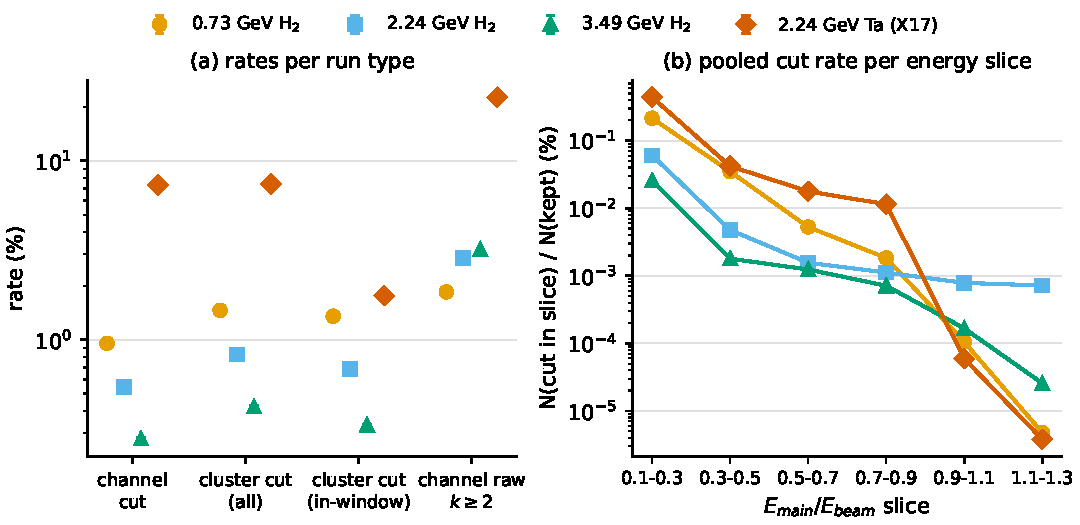
\includegraphics[width=\textwidth]{rates_summary.pdf}
\caption{Pile-up rates per run type. (a) Channel cut rate, cluster cut rate with all extras, cluster cut rate with in-window extras, and raw rate of channels with $K \ge 2$, on a logarithmic axis; the binomial errors are smaller than the markers. (b) Pooled cut rate per slice of $E_{\mathrm{main}}/E_b$: cut channels of the slice divided by all kept, non-vetoed channels of the run type, drawn without error bars. Markers: circle 0.73\,GeV H$_2$, square 2.24\,GeV H$_2$, triangle 3.49\,GeV H$_2$, diamond 2.24\,GeV Ta.}
\label{fig:rates_summary}
\end{figure}

\paragraph{Second pulses.} Figure~\ref{fig:rates_dt} shows $\Delta t$ of the extra in the cut channels. In the hydrogen run types the extra follows the main pulse in 88 to 94\,\% of the cut channels, with a median $\Delta t$ of 11 to 14\,ns and a median $\rho$ of 0.12 to 0.13, both close to the cut values. In the tantalum run type 46.6\,\% of the extras precede the main pulse and the median $|\Delta t|$ is 88\,ns, as expected for pulses that are uncorrelated in time with the main pulse. The in-window cluster rate of tantalum, 1.763\,\%, is about a quarter of the rate with all extras, which is consistent with extras spread over the whole readout. Figure~\ref{fig:rates_grid} gives the two-pulse channels of \code{2p24GeV\_H2} per cell of amplitude ratio and time difference, and Fig.~\ref{fig:rates_examples} shows eight cut channels of that run type.

\begin{figure}[htbp]
\centering
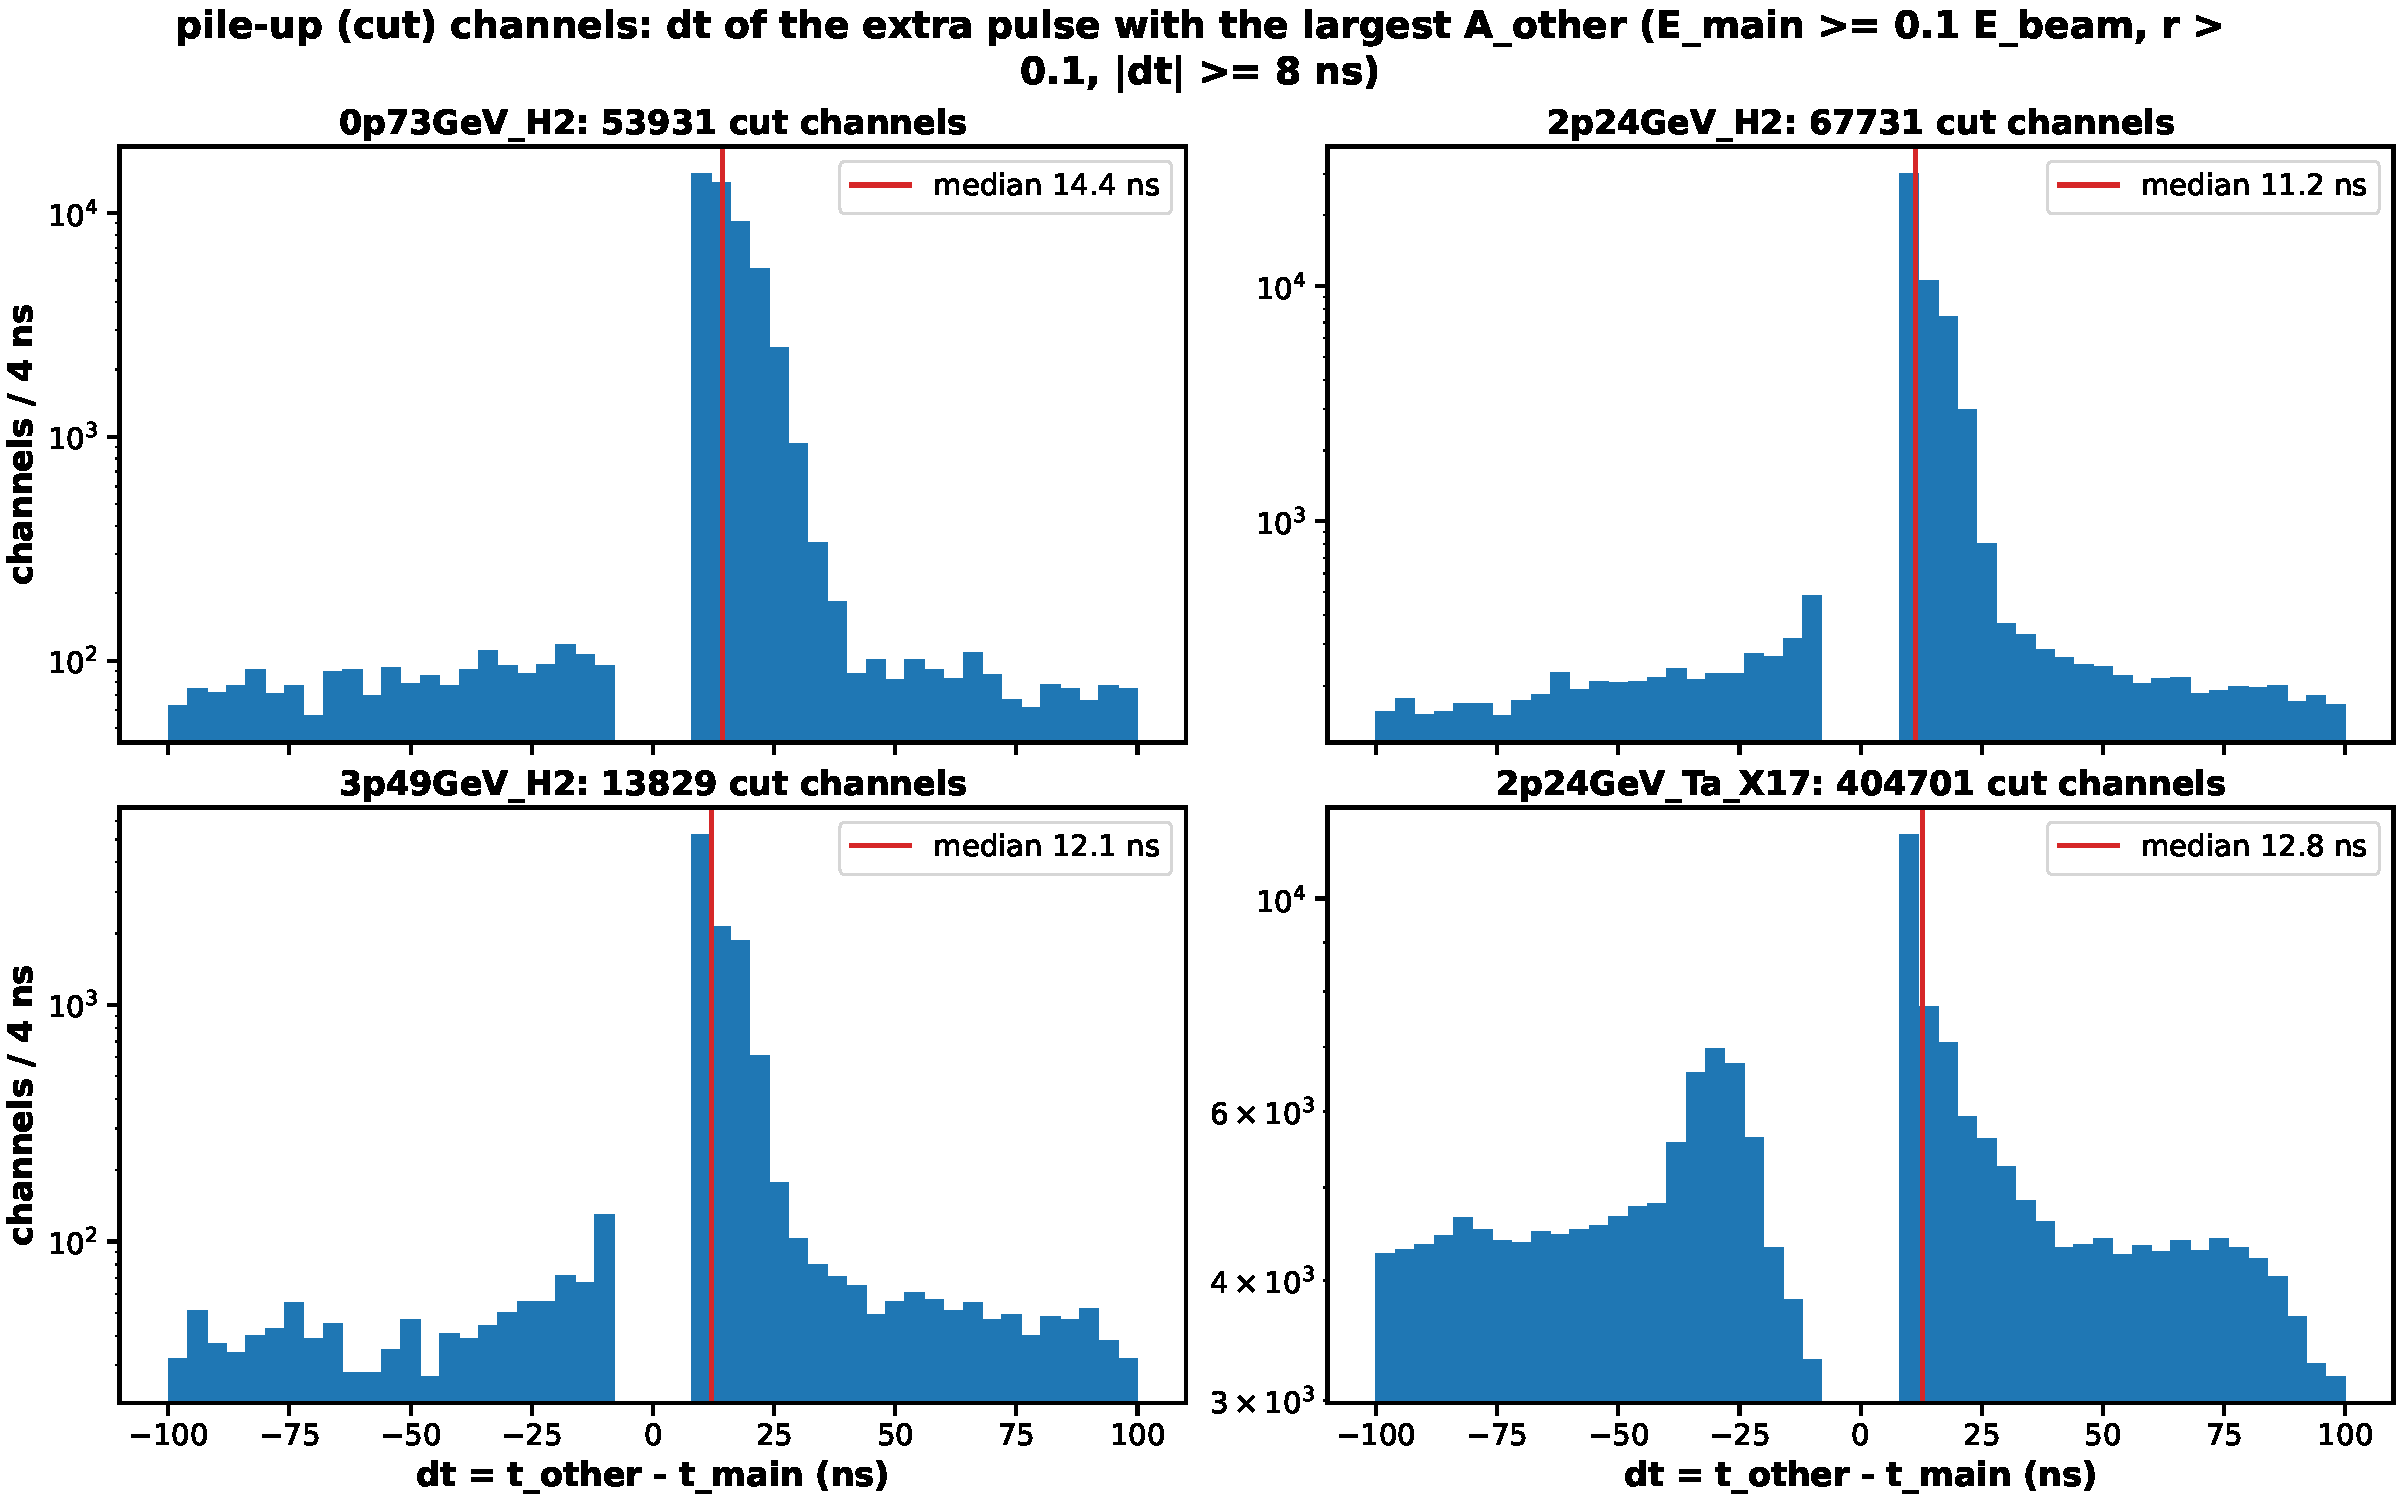
\includegraphics[width=\textwidth]{rates_dt_extra.pdf}
\caption{Time difference $\Delta t = t_{0,n} - t_{0,\mathrm{main}}$ of the extra in the cut channels, one panel per run type, in 4\,ns bins from $-100$ to $100\ns$ on a logarithmic axis. The red line marks the median (14.4, 11.2, 12.1 and 12.8\,ns for 0.73, 2.24, 3.49\,GeV H$_2$ and 2.24\,GeV Ta). The gap at $|\Delta t| < 8\ns$ is the cut of Eq.~\eqref{eq:cutpulse}.}
\label{fig:rates_dt}
\end{figure}

\begin{figure}[htbp]
\centering
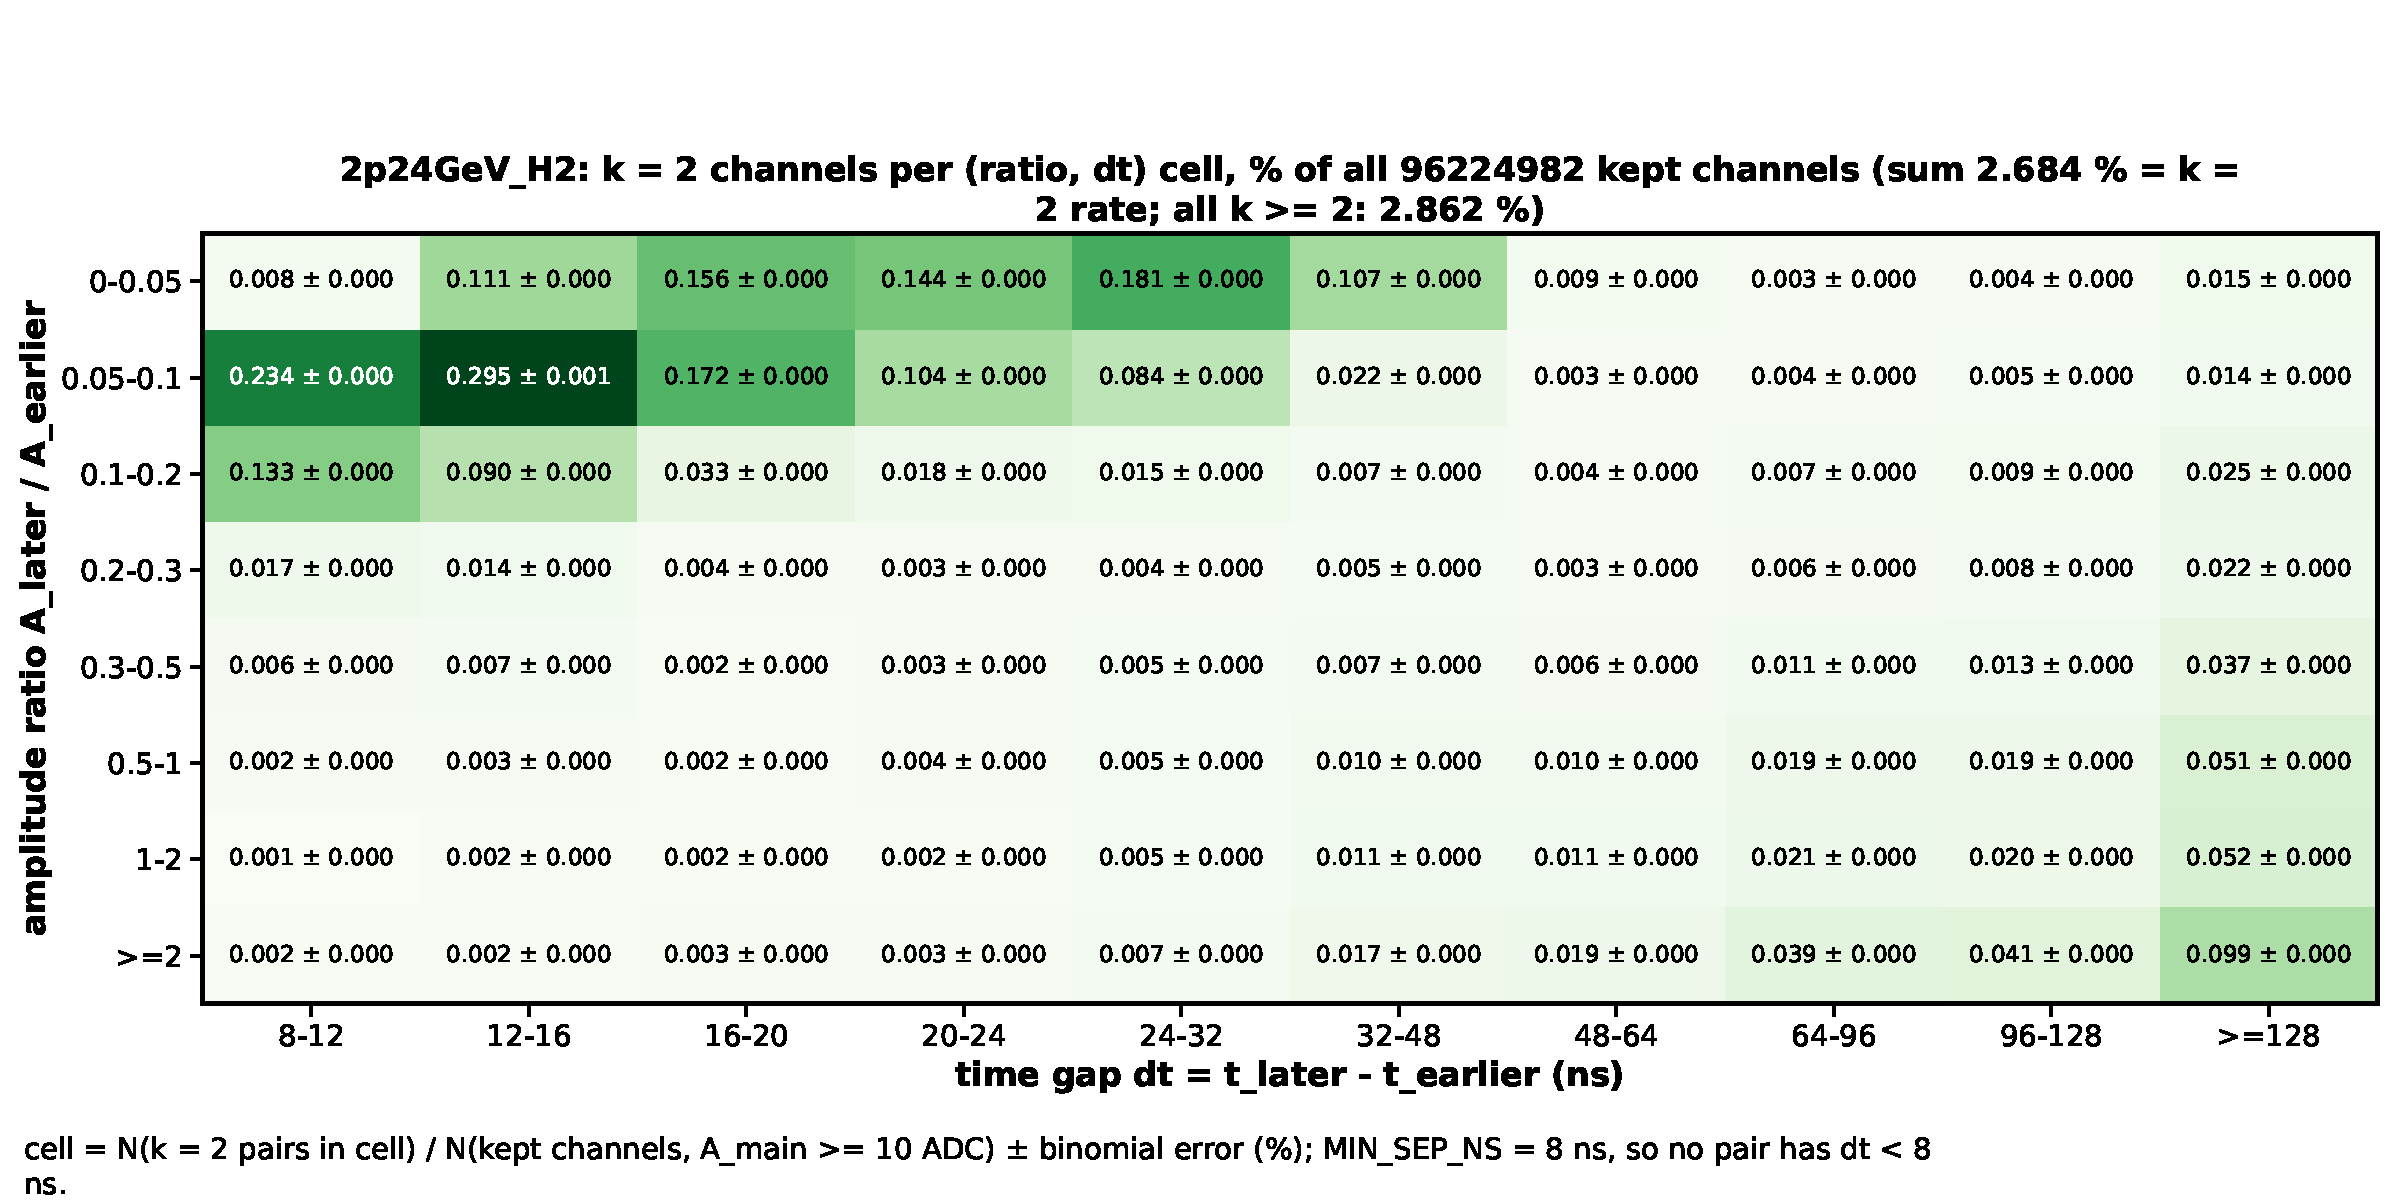
\includegraphics[width=\textwidth]{rates_grid_2p24gev_h2.pdf}
\caption{Channels with $K = 2$ in \code{2p24GeV\_H2} per cell of amplitude ratio (later pulse over earlier pulse) and time difference (later minus earlier), in percent of all 96\,224\,982 kept channels with the binomial error. No energy cut and no veto is applied. The footnote printed on the page states that no pair is closer than 8\,ns; 44\,110 of the 2\,626\,888 channels with $K = 2$ (1.7\,\%) have such a pair (Section~\ref{sec:fitter}, pulse separation) and fall outside the grid.}
\label{fig:rates_grid}
\end{figure}

\begin{figure}[htbp]
\centering
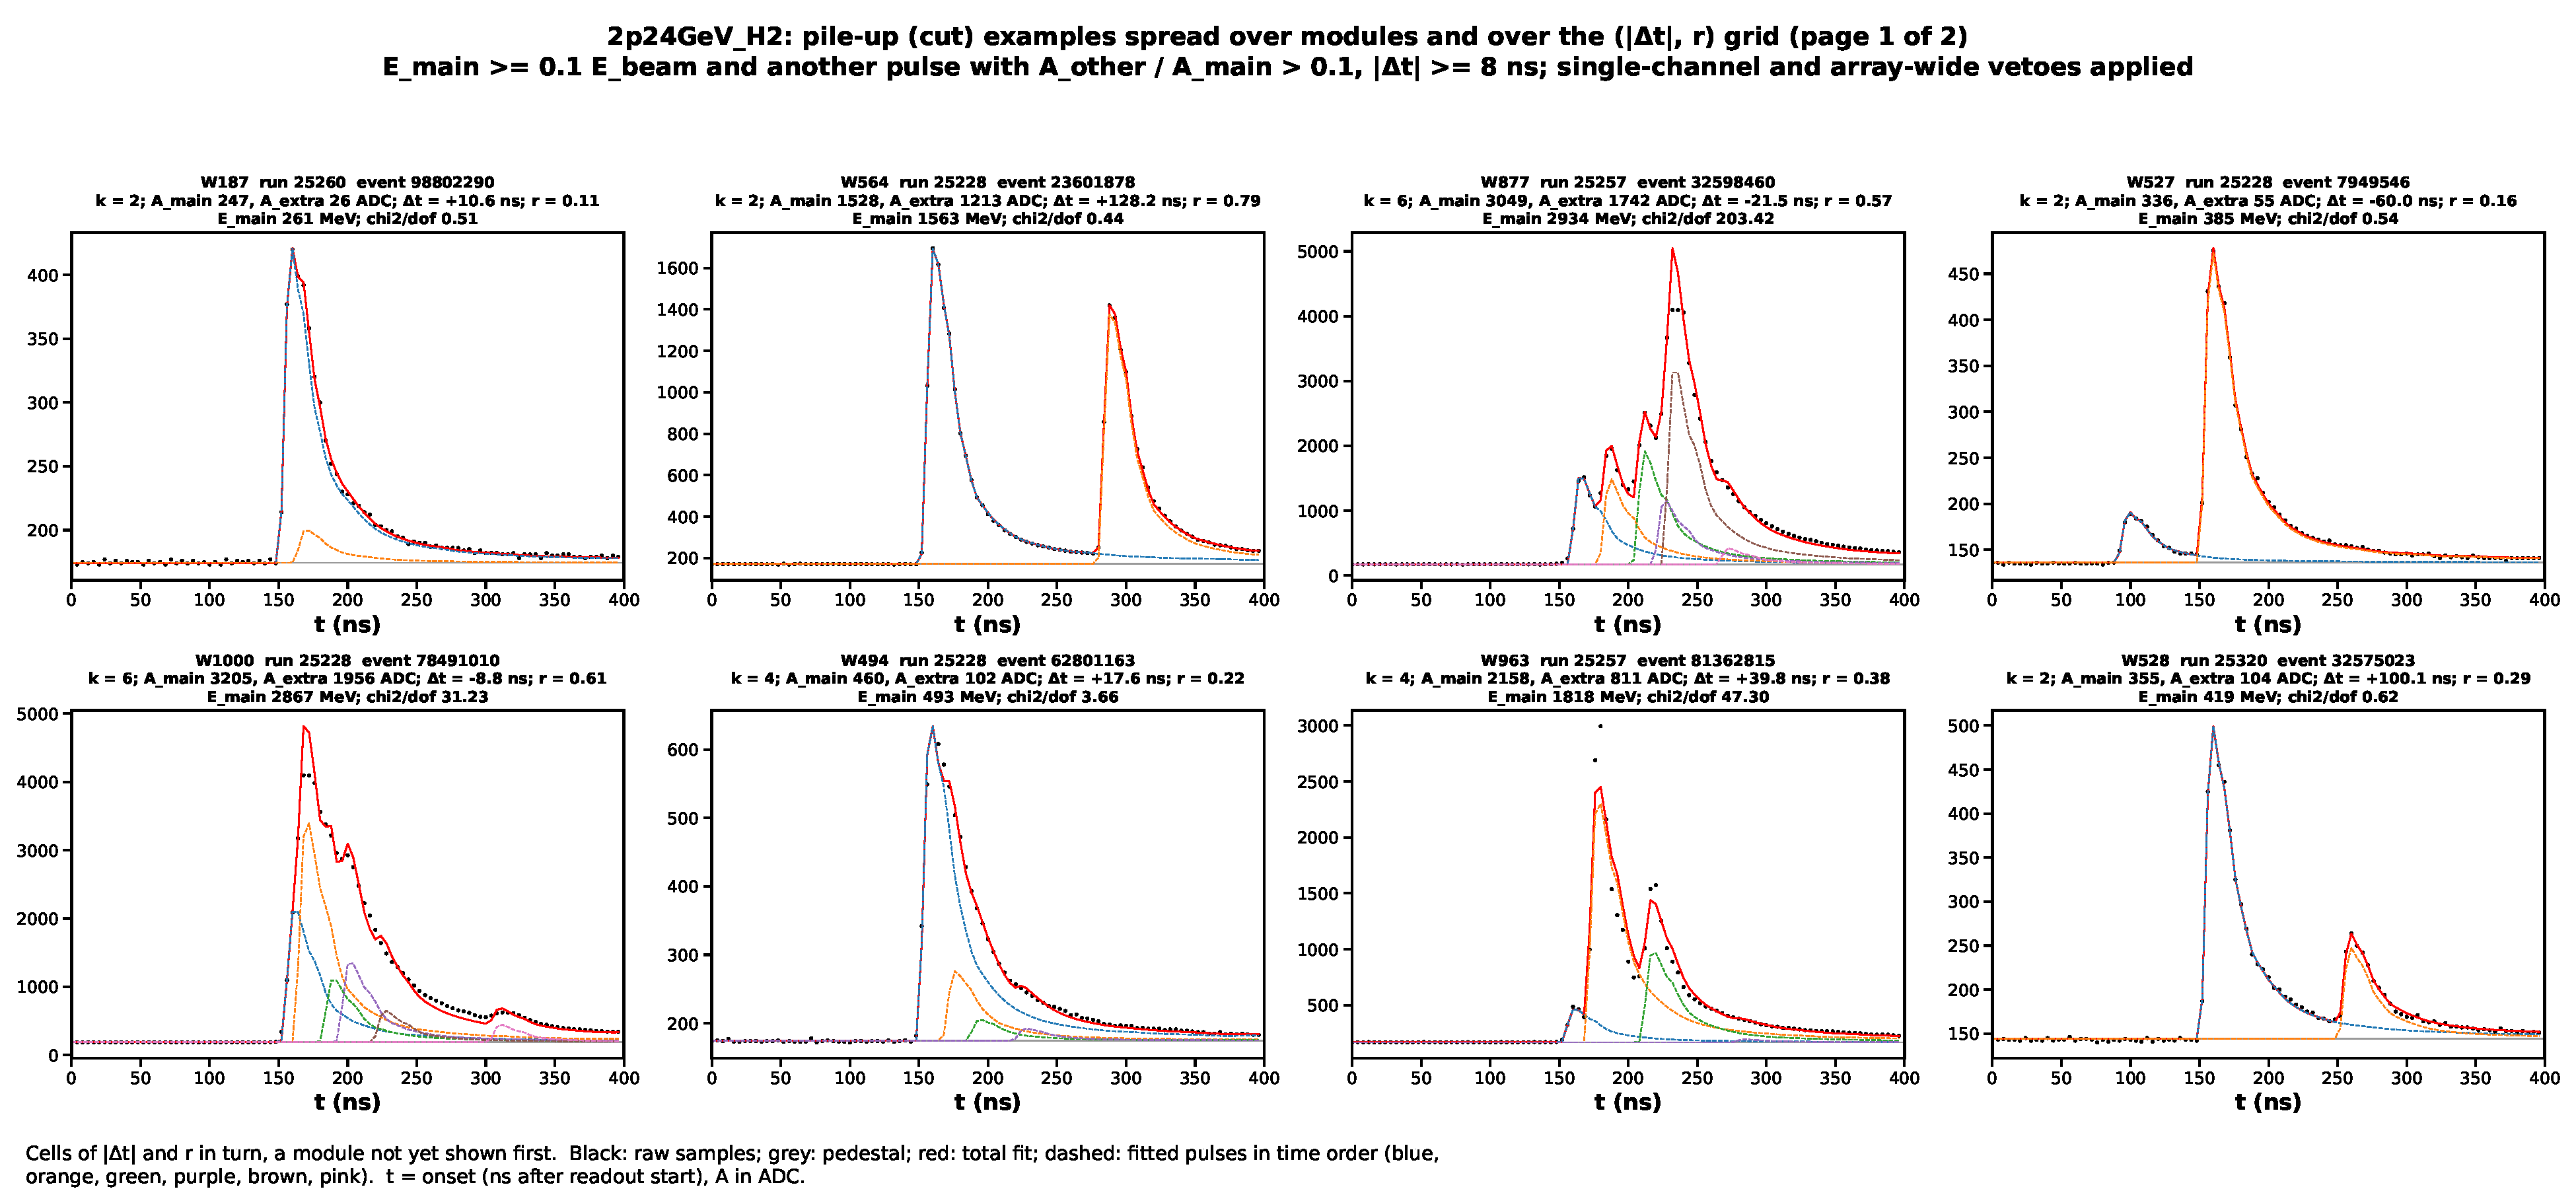
\includegraphics[width=\textwidth]{rates_examples_2p24gev_h2.pdf}
\caption{Eight cut channels of \code{2p24GeV\_H2}, chosen to spread over the cells of $|\Delta t|$ and $\rho$ and over modules, with $K$ from 2 to 6. Black dots: raw samples; grey line: fitted pedestal; red line: total fit; dashed lines: fitted pulses in time order. Horizontal axis: time after the start of the readout (ns); vertical axis: ADC. Each title gives the module, run, event, $K$, $A_{\mathrm{main}}$, the amplitude of the extra, $\Delta t$, $\rho$, $E_{\mathrm{main}}$ and $\chi^2/\mathrm{dof}$.}
\label{fig:rates_examples}
\end{figure}

\paragraph{Hot modules.} Figure~\ref{fig:rates_map} compares the cut rate per module for hydrogen and tantalum at 2.24\,GeV, and Table~\ref{tab:hot} in Appendix~\ref{app:hot} lists the eight hot modules of each run type. In the tantalum run type the hot modules are the eight ring-1 modules that share an edge with the beam hole, with cut rates from 26.0 to 32.3\,\% and raw rates from 55.5 to 59.3\,\%. The four corner modules of ring 1 follow with 11.5 to 14.5\,\%, against a median of 0.43\,\% over all modules. Figure~\ref{fig:rates_w563} shows waveforms of the hottest one, W563. In the hydrogen run types the hot modules lie in rings 9 to 16, at the outer edge of the PbWO$_4$ part, and all but one rest on 101 to 732 channels above threshold. The largest values are W335 at 0.73\,GeV ($208/214 = 97.2 \pm 1.1\,\%$) and W1 at 2.24\,GeV ($159/318 = 50.0 \pm 2.8\,\%$). W335 also has the most saturated channels and bad fits at 0.73\,GeV and is fitted with a single-pulse template; the analysis notes describe it as a ringing channel and as a candidate for the dead list of runs 24590 and 24603.

\begin{figure}[htbp]
\centering
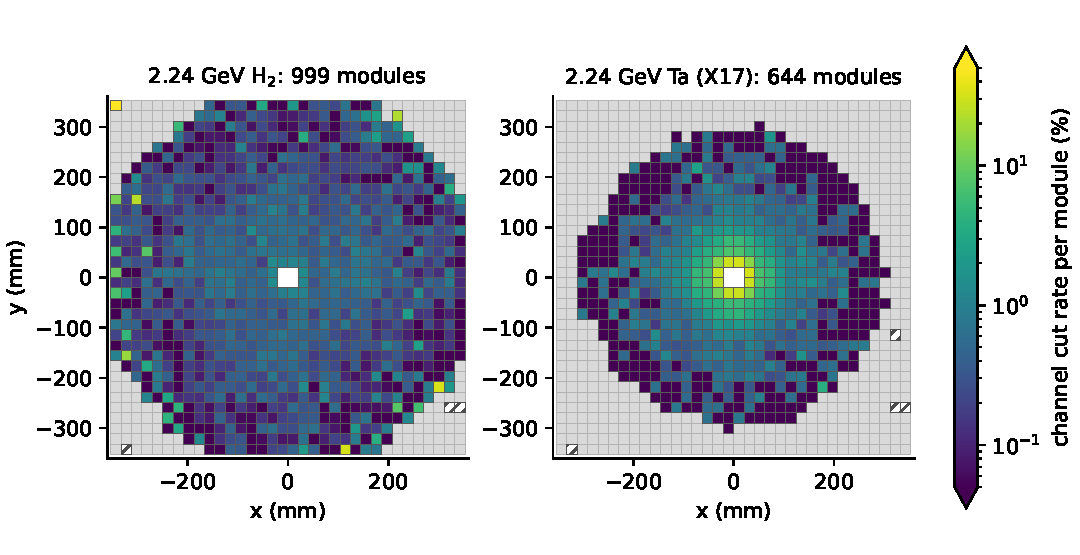
\includegraphics[width=\textwidth]{rates_map_h2_vs_ta.pdf}
\caption{Channel cut rate per PbWO$_4$ module at 2.24\,GeV: hydrogen (left, 999 modules with a value) and tantalum (right, 644 modules). Both panels share one logarithmic colour scale from 0.05 to 50\,\%; values outside are drawn at the ends of the scale. Light grey: fewer than 100 channels above threshold; hatched: dead module. Axes: module position $x$, $y$ (mm).}
\label{fig:rates_map}
\end{figure}

\begin{figure}[htbp]
\centering
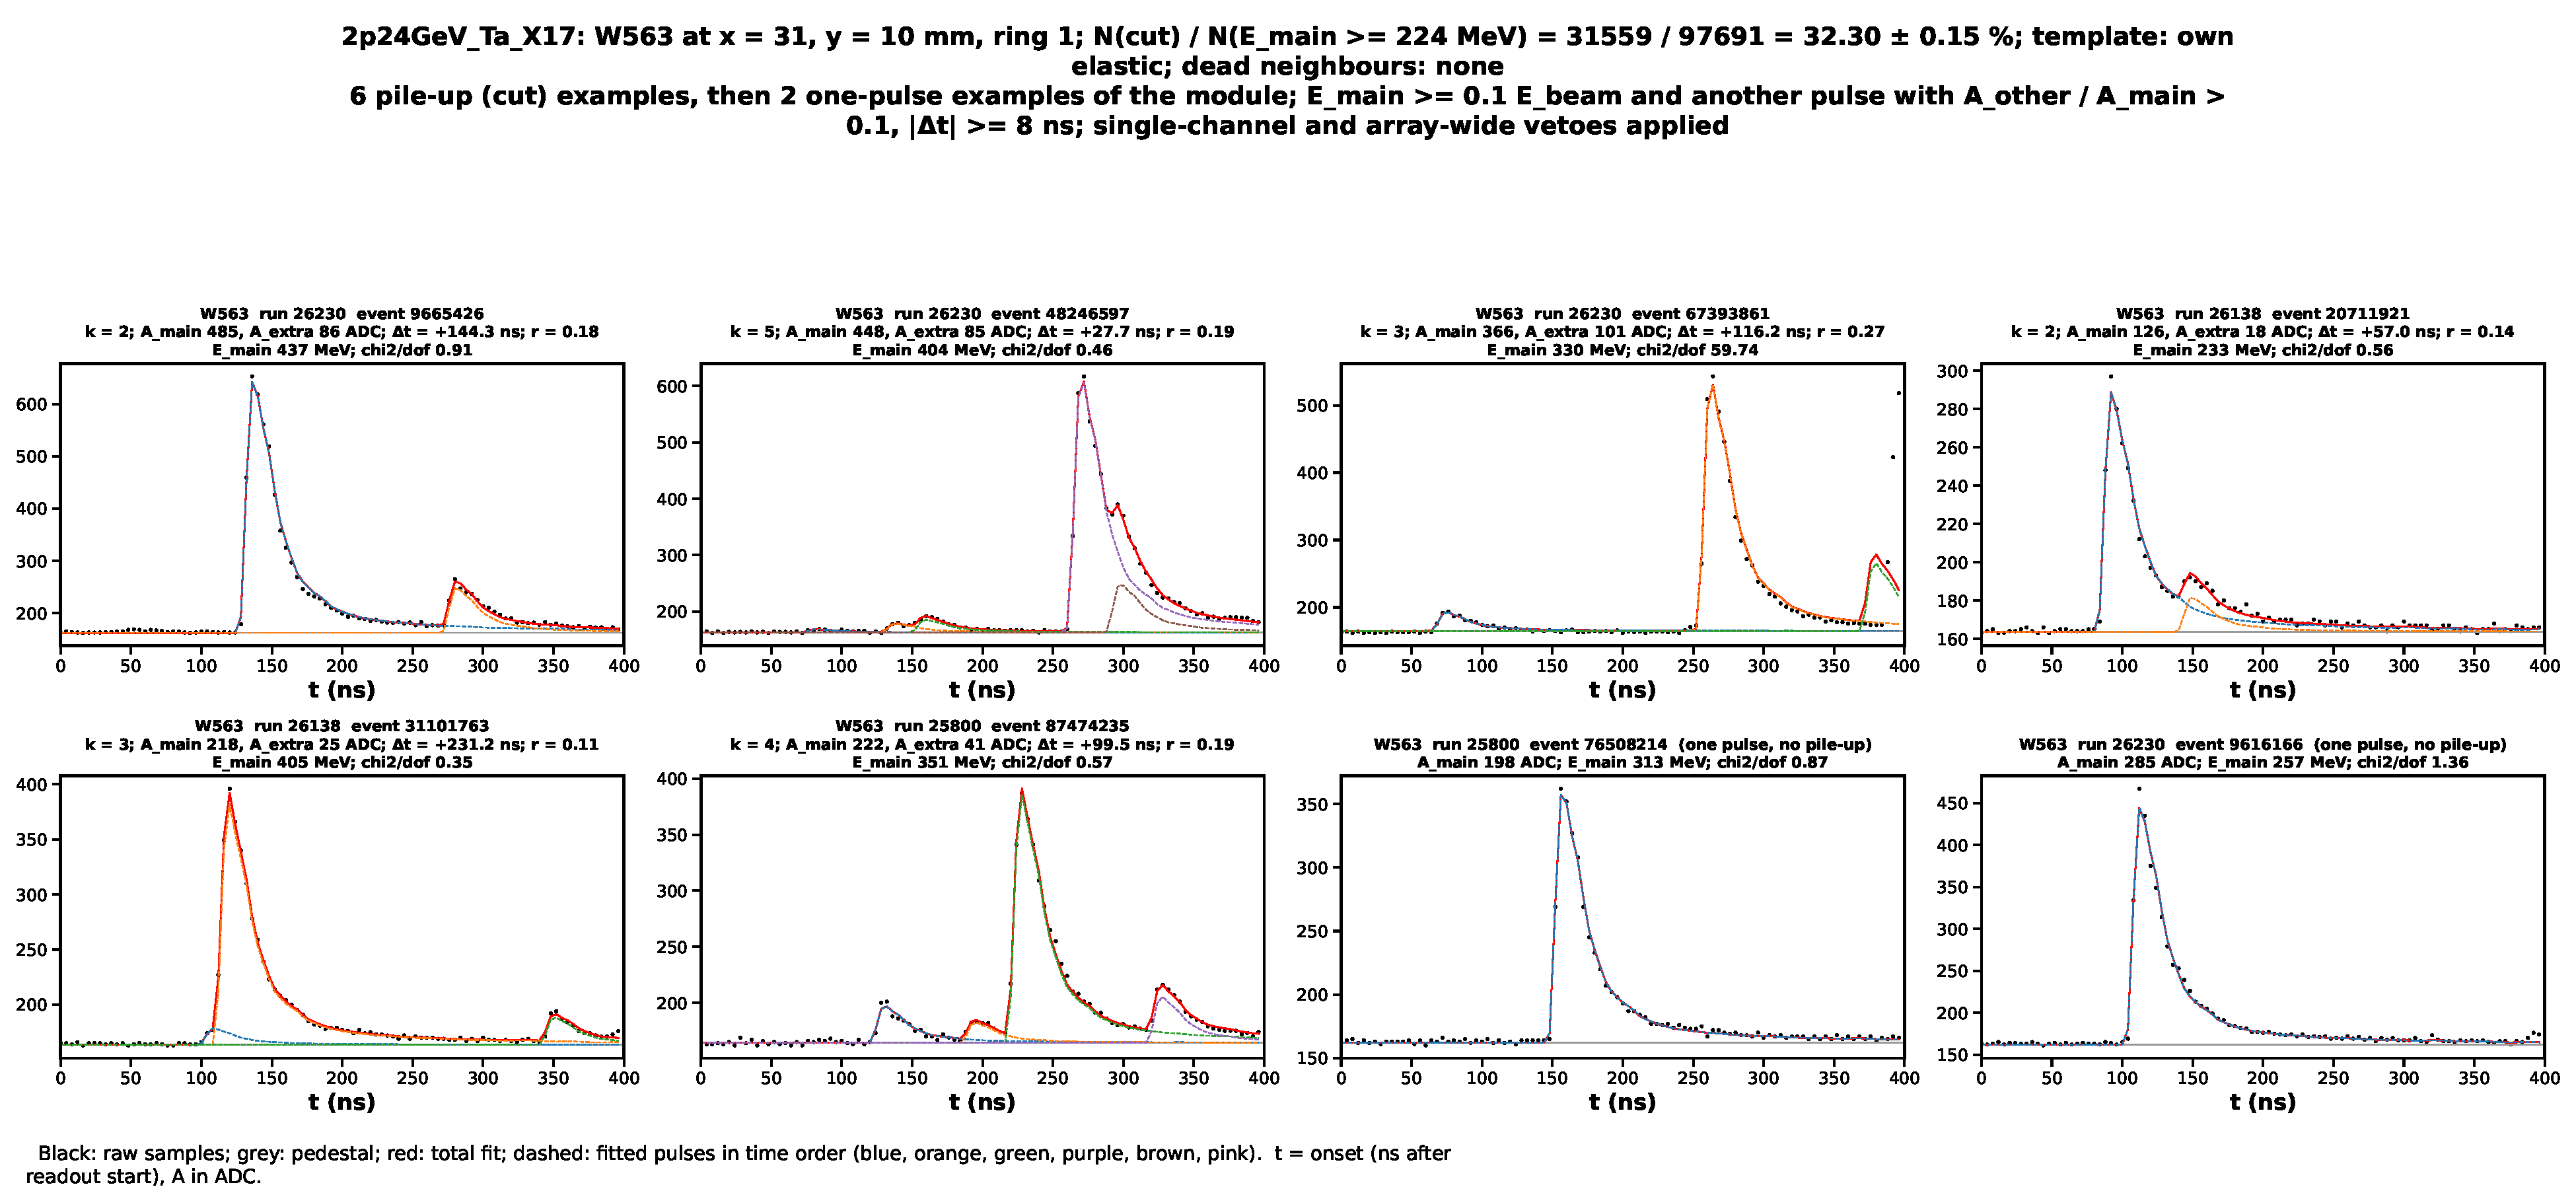
\includegraphics[width=\textwidth]{rates_hot_w563_ta.pdf}
\caption{Waveforms of W563 (ring 1), the hottest module of \code{2p24GeV\_Ta\_X17}, with a cut rate of $31\,559/97\,691 = 32.30 \pm 0.15\,\%$: six cut channels and two one-pulse channels. Black dots: raw samples; grey line: fitted pedestal; red line: total fit; dashed lines: fitted pulses in time order. Horizontal axis: time after the start of the readout (ns); vertical axis: ADC.}
\label{fig:rates_w563}
\end{figure}

\paragraph{Extras of other origin.} Two event displays of run 24590 (\code{0p73GeV\_H2}; script \code{event\_display.py}, numbers from \code{exotic\_events/summary.txt}) show extras that satisfy Eq.~\eqref{eq:cutpulse} and have another origin than a second particle. In event 4\,084\,847 the module W121 is the only read-out module of its $3 \times 3$ neighbourhood (Fig.~\ref{fig:exo_w121}). Its first-30-sample baseline lies $25.2\,\sigma_{\mathrm{ref}}$ above $p_{\mathrm{ref}}$, with an rms of 3.88\,ADC against a median of 0.95\,ADC for this module. The fit starts from $p_{\mathrm{ref}}$, describes the raised baseline with four pulses of 55 to 89\,ADC and reaches $\chi^2/\mathrm{dof} = 127.6$. In the same raw-data file 3 of the 232 read-out waveforms of W121 (1.3\,\%) have a baseline farther than $3\sigma_{\mathrm{ref}}$ from $p_{\mathrm{ref}}$, against 1 of 1344 in the six neighbours with a noise reference. In event 2\,069\,998 the module W493 belongs to a cluster with seed W494 (Fig.~\ref{fig:exo_w493}). Its fit has five pulses with onsets from 154 to 230\,ns and amplitudes falling from 119.8 to 8.2\,ADC, at $\chi^2/\mathrm{dof} = 1.15$. The three read-out neighbours carry one pulse each, with onsets from 148 to 151\,ns, so the extras of W493 are read as a pulse wider than the template of the module. Section~\ref{sec:exotic} defines flags for such waveforms and measures their rates and their effect on clusters and yields.

\begin{figure}[htbp]
\centering
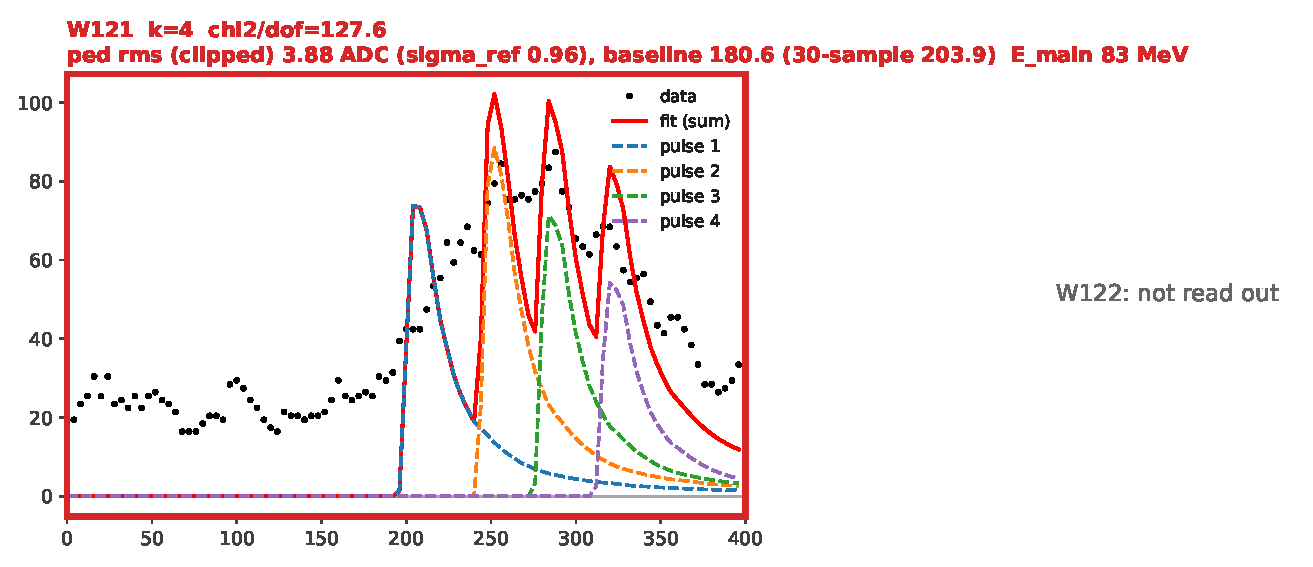
\includegraphics[width=0.62\textwidth]{exotic_w121_baseline_burst.pdf}
\caption{W121 in event 4\,084\,847 of run 24590, fitted with $K = 4$ at $\chi^2/\mathrm{dof} = 127.6$. Black dots: raw samples minus the fitted pedestal; red line: total fit; dashed lines: fitted pulses in time order. None of the eight neighbours was read out (label of W122 at the right). Horizontal axis: time after the start of the readout (ns); vertical axis: ADC.}
\label{fig:exo_w121}
\end{figure}

\begin{figure}[htbp]
\centering
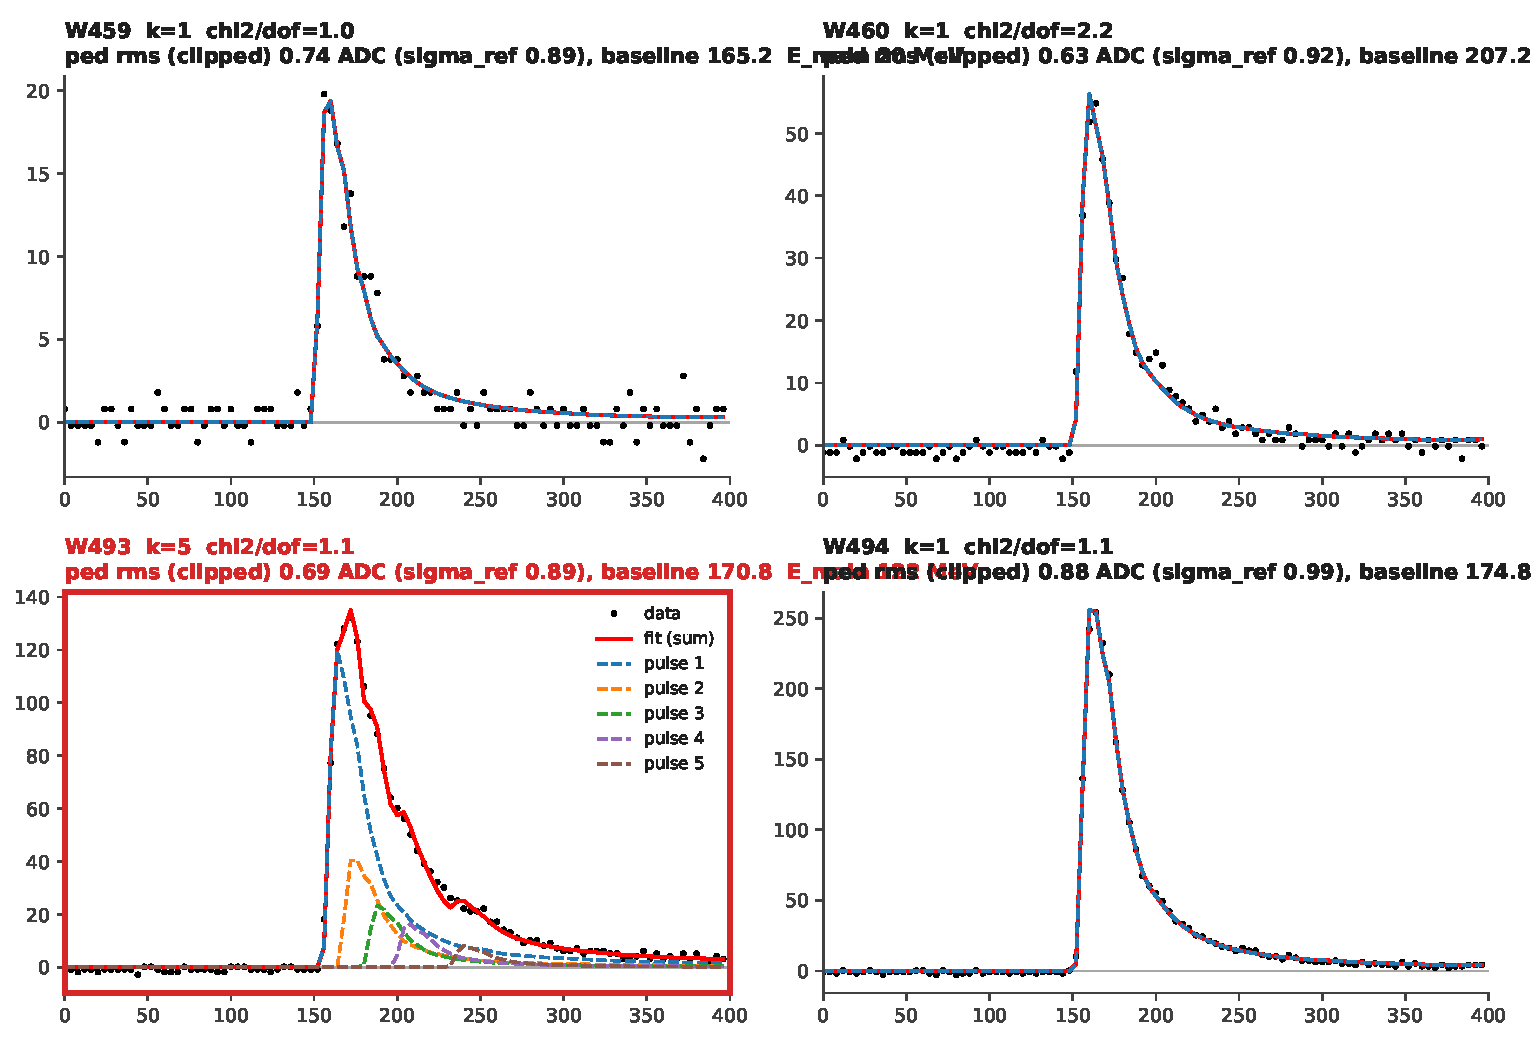
\includegraphics[width=0.85\textwidth]{exotic_w493_wide_pulse.pdf}
\caption{Event 2\,069\,998 of run 24590: W493 (red frame, $K = 5$) and its three read-out neighbours W459, W460 and W494, each with $K = 1$. The panels are placed as the modules, with $x$ to the right and $y$ up, and each has its own vertical range. Lines and axes as in Fig.~\ref{fig:exo_w121}.}
\label{fig:exo_w493}
\end{figure}

\paragraph{Limits of the numbers.} Four properties of the counting bound what the rates mean.
\begin{itemize}
\item The hydrogen extras sit just above both cuts, 10 to 14\,ns after the main pulse with $\rho$ near 0.12. A fluctuation of the pulse shape on the falling edge gives the same signature, so the hydrogen cut rates are read as upper limits on the pile-up.
\item The pooled slice rate is a fraction of all kept channels. It is not the pile-up probability of a channel inside the slice.
\item The cluster numerator accepts any member above threshold, while the denominator requires the seed above threshold. The size of this asymmetry is not determined.
\item Several hot-module waveforms of the hydrogen run types are pulses of 1600 to 3200\,ADC fitted with $K = 5$ or 6 and $\chi^2/\mathrm{dof}$ from 27 to 476. Whether these are pile-up or a template that does not describe the module is not determined. Ten of the 16 hot modules at 0.73 and 3.49\,GeV rest on 2 to 7 cut channels, with relative errors of 37 to 71\,\%.
\end{itemize}
One further count is recorded without an explanation. At 3.49\,GeV 49\,612 events (1.97\,\%) have a kept channel and no in-window pulse, against 8 to 216 events in the other run types.
\clearpage

\subsection{Pile-up generator}
\label{sec:generator}

\paragraph{Purpose, inputs, outputs.} The generator writes synthetic one- and two-pulse waveforms whose amplitudes and onsets are known exactly, so that the fitter can be measured against the truth (Section~\ref{sec:deconv}). Its only input is the template bank of \code{2p24GeV\_H2}: the spline $f$, \code{shape\_sigma} and \code{a\_band} of five modules. No data are read. Its output is one file, \code{pileup\_stage1.npz}, with the waveforms and the truth of every event. The script is \code{pileup\_generator\_stage1.py}.

\subsubsection{Procedure}

\begin{enumerate}
\item \textbf{Modules.} Five modules of ring 2 are used: W493, W564, W664, W593 and W494. Their pedestal $p_{\mathrm{gen}}$ and noise $\sigma_{\mathrm{gen}}$ are fixed in the script (Table~\ref{tab:gen}).
\item \textbf{Template tables.} The spline of each module is tabulated every 0.05\,ns (\code{LUT\_DT}) and interpolated linearly, with $f(\tau) = 0$ outside $0 < \tau < 400\ns$. The peak time $t_{\mathrm{pk}}$ is the time of the table maximum and $t_{50}$ the first crossing of half the maximum on the leading edge. One template serves both pulses of an event.
\item \textbf{Shape perturbation.} The pulse-to-pulse scatter of the shape is generated in the B-spline basis $B_l(\tau)$ of the module (Section~\ref{sec:lsq}). Each coefficient $l$ receives a Gaussian deviate $\zeta_l$ scaled by $\sigma_s$ at its Greville abscissa $\gamma_l$, the mean of the three interior knots of $B_l$:
\begin{equation}
\delta f(\tau) = \alpha\, \sqrt{\frac{a_{\mathrm{band}}}{A_1}}\, \sum_l B_l(\tau)\, \sigma_s(\gamma_l)\, \zeta_l
\quad (0 < \tau < 250\ns),
\qquad
\delta f(\tau) = 0 \ \text{otherwise}.
\label{eq:deltaf}
\end{equation}
The scale $\alpha$ makes the standard deviation of the sum equal to $\sigma_s$ on average over the two points $t_{\mathrm{pk}}$ and $t_{50}$:
\begin{equation}
\alpha = \Big[ \tfrac{1}{2} \sum_{\tau \in \{t_{\mathrm{pk}},\, t_{50}\}} \frac{\sum_l B_l(\tau)^2\, \sigma_s(\gamma_l)^2}{\sigma_s(\tau)^2} \Big]^{-1/2} .
\label{eq:alpha}
\end{equation}
The factor $\sqrt{a_{\mathrm{band}}/A_1}$ scales the scatter from the amplitude at which it was measured to the amplitude of the primary pulse, as in Eq.~\eqref{eq:vj}. The perturbation is tabulated every 0.2\,ns (\code{SMEAR\_DT}) up to 250\,ns (\code{SMEAR\_TMAX}) with strength 1 (\code{SMEAR\_K}).
\item \textbf{Grid.} A combination is a module, a primary amplitude $A_1$, a ratio $\rho = A_2/A_1$ and a time difference $\Delta t = t_2 - t_1$, with the values of Table~\ref{tab:gen}; $\rho = 0$ is the one-pulse control. A negative $\Delta t$ places the secondary pulse first. A combination is dropped when its noiseless, unperturbed waveform at the nominal onset exceeds $4095\adc - 4\sigma_{\mathrm{gen}}$ at its maximum.
\item \textbf{Event assignment.} Event number $e$ receives combination $e$ modulo the number of kept combinations, so every combination gets the same number of events when the total is a multiple of that number.
\item \textbf{Truth.} The primary onset is $t_1 = 152\ns + U$ with $U$ uniform in $[0, 4)\ns$ (\code{T1\_NS}), which samples every phase of the 4\,ns clock. The secondary pulse has $t_2 = t_1 + \Delta t$ and $A_2 = \rho A_1$.
\item \textbf{Waveform.} With Gaussian deviates $z_j$ for the noise, the 100 samples are
\begin{equation}
s_j = \operatorname{round}\Big( p_{\mathrm{gen}} + \sigma_{\mathrm{gen}} z_j + A_1\, [f + \delta f](t_j - t_1) + A_2\, [f + \delta f](t_j - t_2) \Big) .
\label{eq:genwave}
\end{equation}
Both pulses of an event carry the same realisation of $\delta f$, and the peak is not renormalised after the perturbation.
\item \textbf{Overflow.} No sample is clipped. An event with a sample at or above 4095\,ADC is drawn again, with new noise and a new perturbation and the same truth.
\item \textbf{Storage.} The file holds per event the waveform, the module, $A_1$, $A_2$, $\rho$, $\Delta t$, $t_1$, $t_2$, $p_{\mathrm{gen}}$, $\sigma_{\mathrm{gen}}$ and the rms of $\delta f$ over the pulse (\code{smear\_rms}), plus one metadata record with the grid, the seed (\code{SEED} $= 12345$) and the SHA-1 checksum of the bank. The pulse components and $\delta f$ themselves are not stored.
\end{enumerate}

\begin{table}[htbp]
\centering
\caption{Grid and module constants of the generator. The last two columns of the lower block are read from the bank and the metadata of the file.}
\label{tab:gen}
\small
\begin{tabular}{lp{0.60\textwidth}l}
\toprule
Quantity & Values & Constant \\
\midrule
$A_1$ (ADC) & 300, 1000, 3000 & \code{A1\_ADC} \\
$\rho$ & 0 (control), 0.05, 0.1, 0.2, 0.3, 0.5, 1, 2 & \code{RATIOS} \\
$\Delta t$ (ns) & $\pm 8$, $\pm 12$, $\pm 16$, $\pm 20$, $\pm 24$, $\pm 32$, $\pm 48$, $\pm 64$, $\pm 96$, $\pm 128$ & \code{DT\_NS} \\
Samples, period & 100 samples of 4\,ns & \code{NSAMP}, \code{CLK\_NS} \\
\bottomrule
\end{tabular}

\medskip
\begin{tabular}{lrrrr}
\toprule
Module & $p_{\mathrm{gen}}$ (ADC) & $\sigma_{\mathrm{gen}}$ (ADC) & $a_{\mathrm{band}}$ (ADC) & $\alpha$ \\
\midrule
W493 & 170.18 & 0.84 & 450.0 & 1.453 \\
W564 & 170.21 & 0.92 & 472.7 & 1.437 \\
W664 & 183.40 & 0.89 & 470.4 & 1.431 \\
W593 & 145.14 & 0.81 & 492.9 & 1.433 \\
W494 & 173.81 & 0.88 & 451.6 & 1.425 \\
\bottomrule
\end{tabular}
\end{table}

\subsubsection{Results}

\paragraph{Generated sample.} The file used in Section~\ref{sec:deconv} was written with 19\,510\,000 events. The grid has 141 pairs of $\rho$ and $\Delta t$ (the control and $7 \times 20$ two-pulse pairs), three amplitudes and five modules, which gives 2115 combinations. The drop rule removes 164 of them, all at $A_1 = 3000\adc$, and 1951 remain, each with 10\,000 events; 150\,000 events are controls. The templates of the five modules peak at $t_{\mathrm{pk}} = 11.15$ to 11.45\,ns and reach half maximum at $t_{50} = 4.88$ to 4.98\,ns. For W493 the rms over 2000 check draws of the template error over the two calibration points is 1.78\,\% of the peak at $A_1 = 300\adc$, 0.98\,\% at 1000\,ADC and 0.56\,\% at 3000\,ADC, against targets of 1.82, 1.00 and 0.58\,\%. Figure~\ref{fig:gen_examples} shows six generated events with their truth.

\begin{figure}[htbp]
\centering
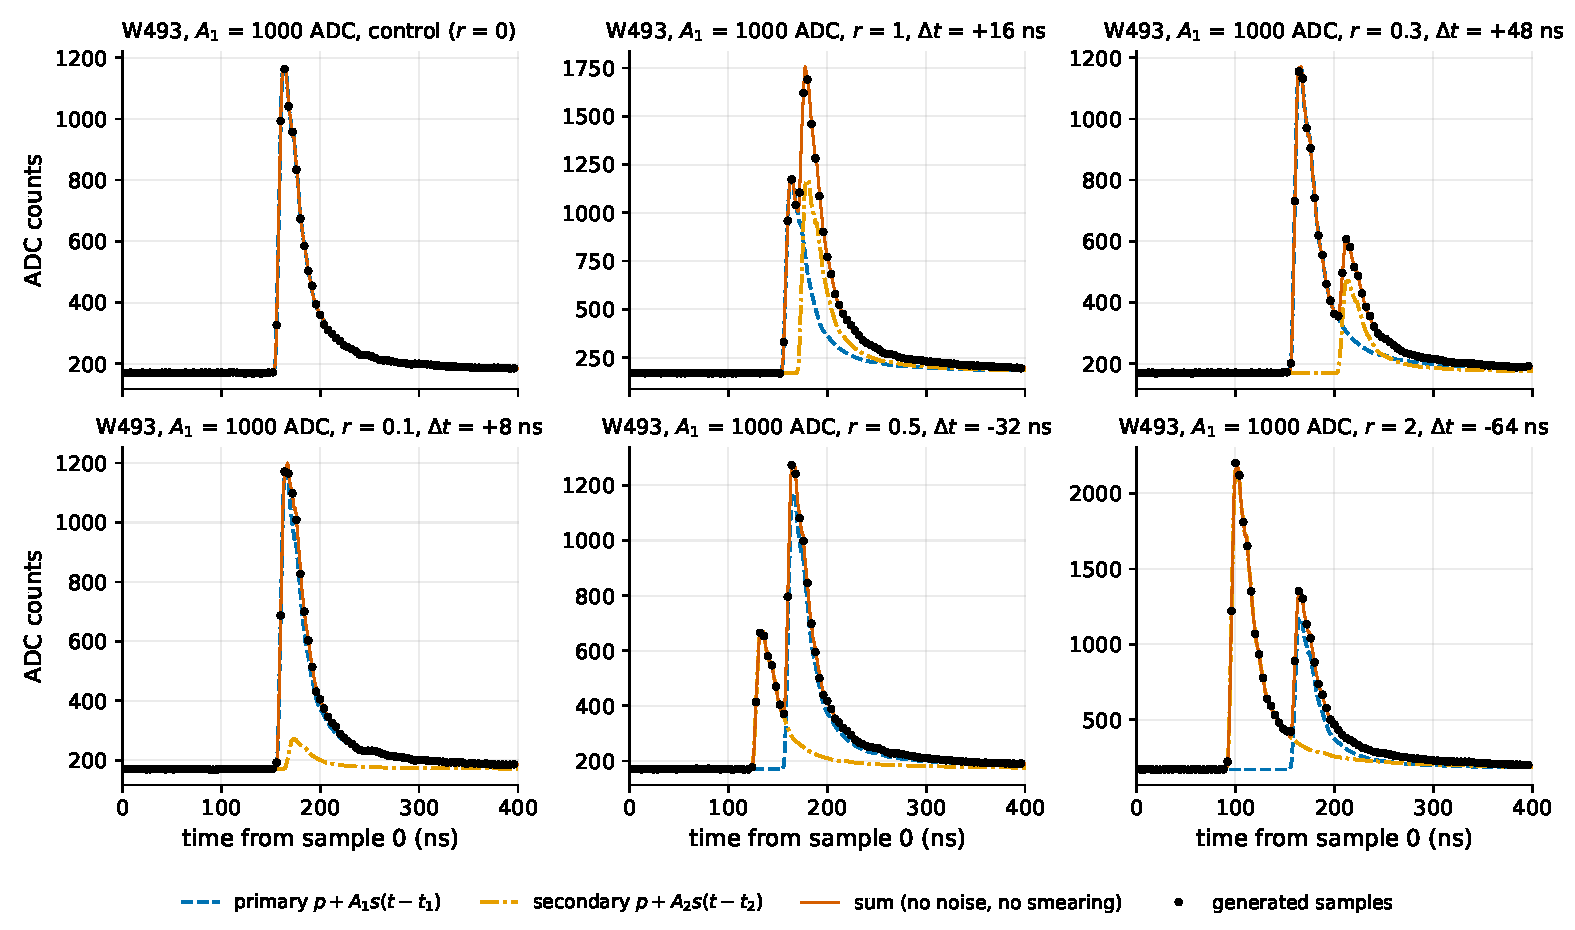
\includegraphics[width=\textwidth]{gen_examples.pdf}
\caption{Six generated waveforms of W493 at $A_1 = 1000\adc$: the control and the pairs $(\rho, \Delta t) = (1, +16\ns)$, $(0.3, +48\ns)$, $(0.1, +8\ns)$, $(0.5, -32\ns)$ and $(2, -64\ns)$, the first event of each combination. Black dots: generated samples, pedestal included. Blue dashed line: true primary pulse, $p_{\mathrm{gen}} + A_1 f(t - t_1)$. Orange dash-dotted line: true secondary pulse. Red solid line: their sum. The curves are drawn on a 0.1\,ns grid from the stored truth and the present bank, without noise and without $\delta f$, which is not stored. Horizontal axis: time after sample 0 (ns); vertical axis: ADC.}
\label{fig:gen_examples}
\end{figure}

\paragraph{Limits of the model.} The noise is white; the correlation between neighbouring samples of the real noise, about $-0.3$, is not generated. Both pulses share one $\delta f$ scaled with $A_1$, so the shape error of the secondary pulse does not follow its own amplitude. For $\Delta t \le -48\ns$ the secondary pulse starts inside the first 30 samples, the window from which the fitter takes its baseline and noise. The events depend on the seed, on the number of events and on the chunk size of 100\,000 events (\code{CHUNK}). The bank file with the checksum stored in the metadata is no longer on disk. The present bank, rebuilt on 2026-11-12, has the same splines, \code{shape\_sigma} and \code{a\_band} for the five modules, but its checksum differs.

\subsection{Deconvolution study}
\label{sec:deconv}

\paragraph{Purpose, inputs, outputs.} The deconvolution study measures how often the fitter of Section~\ref{sec:fitter} recovers a known second pulse, how often it invents one, and how much a second pulse disturbs the amplitude of the main pulse. Its inputs are the generated file of Section~\ref{sec:generator} and the template bank that produced it. Its outputs are \code{efficiency.tsv}, with one row per combination of module, $A_1$, $\rho$ and $\Delta t$, a PDF of efficiency tables and a PDF of example fits. The script is \code{pileup\_deconvolution\_study.py}.

\subsubsection{Procedure}

\begin{enumerate}
\item \textbf{Inputs.} The script reads the waveforms and the truth, and stops when the SHA-1 checksum of the bank file differs from the one stored by the generator.
\item \textbf{Fit.} Every waveform passes steps 1 to 10 of Section~\ref{sec:fitter} with the noise of step 2, measured on its own first 30 samples. The fitter knows nothing of the truth. Two of its constants bound what the generated grid can test. The candidate separation of 8\,ns (\code{MIN\_SEP\_NS}) equals the smallest generated $|\Delta t|$. The residual-pulse floor of 0.02 (\code{R\_MODEL}) lies below the smallest generated $\rho$ of 0.05.
\item \textbf{Matching.} The fitted main pulse, with onset $\hat t_{\mathrm{main}}$ and amplitude $\hat A_{\mathrm{main}}$, is the valid fitted pulse closest in onset to $t_1$; no tolerance is applied. The fitted secondary pulse ($\hat t_{\mathrm{sec}}$, $\hat A_{\mathrm{sec}}$) is the valid pulse closest to $t_2$ among the others. The assignment follows the true onsets, so it holds for either sign of $\Delta t$.
\item \textbf{Event quantities.} Table~\ref{tab:deconvdef} defines the quantities of an event. A secondary pulse is found when it passes both the timing and the amplitude tolerance.
\item \textbf{Cell statistics.} A cell is one combination and holds $N_{\mathrm{cell}} = 10\,000$ events. The efficiency is $\varepsilon = N_{\mathrm{found}}/N_{\mathrm{cell}}$ with the binomial error $\sqrt{\varepsilon (1 - \varepsilon)/N_{\mathrm{cell}}}$. In a control cell the false-positive rate is the fraction of events with two or more fitted pulses. The timing and amplitude residuals of a cell are summarised by their median and 1.4826 times their MAD over the events that pass the timing tolerance. The pull is summarised over the found events, and over the one-pulse events in a control cell.
\end{enumerate}

\begin{table}[htbp]
\centering
\caption{Event quantities of the deconvolution study. A hat marks a fitted value; $p_{\mathrm{gen}}$ and $\sigma_{\mathrm{gen}}$ are the generated pedestal and noise.}
\label{tab:deconvdef}
\small
\begin{tabular}{lll}
\toprule
Quantity & Definition & Constant \\
\midrule
Timing residual & $\hat t_{\mathrm{sec}} - t_2$ & \\
Amplitude residual & $\hat A_{\mathrm{sec}}/A_2 - 1$ & \\
Timing tolerance & $|\hat t_{\mathrm{sec}} - t_2| \le 4\ns$ & \code{T\_TOL\_NS} \\
Amplitude tolerance & $|\hat A_{\mathrm{sec}}/A_2 - 1| \le 0.30$ & \code{A\_TOL} \\
Found & timing and amplitude tolerance passed & \\
Main-pulse pull & $\hat A_{\mathrm{main}}/A_1 - 1$ & \\
Pedestal bias & (fitted pedestal $- p_{\mathrm{gen}}$)$/\sigma_{\mathrm{gen}}$ & \\
$\chi^2/\mathrm{dof}$ & Eq.~\eqref{eq:mfchi2} with $\sigma = \sigma_{\mathrm{gen}}$ & \\
\bottomrule
\end{tabular}
\end{table}

\subsubsection{Results}

\paragraph{Efficiency.} Table~\ref{tab:eff} and Fig.~\ref{fig:deconv_eff} give the efficiency pooled over the five modules. The earliest onsets ($\Delta t \le -96\ns$) are treated in a separate paragraph below. At every other $\Delta t$ and every $A_1$, a secondary pulse with $\rho \ge 0.2$ is found in at least 95.4\,\% of the events, and one with $\rho \ge 0.3$ in at least 99.6\,\%. At $\rho = 0.1$ the efficiency at $\Delta t = +8\ns$ is 49.1, 83.4 and 97.0\,\% for $A_1 = 300$, 1000 and 3000\,ADC, and it is at least 92.9\,\% from $|\Delta t| = 12\ns$ on. At $\rho = 0.05$ a secondary pulse at $\pm 8\ns$ is not resolved (0.0 to 1.3\,\%), and at $A_1 = 300\adc$ and positive $\Delta t$ the efficiency reaches 90\,\% only between $+32$ and $+48\ns$. At $\rho \le 0.1$ and $|\Delta t| \le 12\ns$ a resolved secondary pulse ahead of the primary one is found more often than one behind it (56.7 against 29.2\,\% at $\rho = 0.05$, $|\Delta t| = 12\ns$ and $A_1 = 300\adc$). Of the 1936 two-pulse cells, 49 have an efficiency below 50\,\%, 117 below 90\,\% and 165 below 99\,\%. Figure~\ref{fig:deconv_examples} shows two found and two missed secondary pulses, and Fig.~\ref{fig:deconv_control} a control event.

\begin{table}[htbp]
\centering
\caption{Efficiency (\%) to find the secondary pulse, pooled over the five modules (50\,000 events per entry), from \code{efficiency.tsv}. The binomial errors are at most 0.22\,\%. For $\rho \ge 0.3$ every entry at these $\Delta t$ is at least 99.6\,\%.}
\label{tab:eff}
\small
\begin{tabular}{rrrrrrrrrr}
\toprule
$A_1$ (ADC) & $\rho$ & $-12\ns$ & $-8\ns$ & $+8\ns$ & $+12\ns$ & $+16\ns$ & $+24\ns$ & $+32\ns$ & $+48\ns$ \\
\midrule
300 & 0.05 & 56.7 & 0.0 & 1.3 & 29.2 & 60.5 & 81.5 & 87.3 & 97.1 \\
300 & 0.1 & 100.0 & 84.6 & 49.1 & 92.9 & 98.7 & 99.8 & 99.9 & 100.0 \\
300 & 0.2 & 100.0 & 99.9 & 95.4 & 100.0 & 100.0 & 100.0 & 100.0 & 100.0 \\
1000 & 0.05 & 91.7 & 0.0 & 0.5 & 65.0 & 97.3 & 99.6 & 99.8 & 100.0 \\
1000 & 0.1 & 100.0 & 97.7 & 83.4 & 99.8 & 100.0 & 100.0 & 100.0 & 100.0 \\
3000 & 0.05 & 97.6 & 0.0 & 0.0 & 85.9 & 99.9 & 99.9 & 100.0 & 100.0 \\
3000 & 0.1 & 100.0 & 99.5 & 97.0 & 99.9 & 100.0 & 99.9 & 100.0 & 100.0 \\
\bottomrule
\end{tabular}
\end{table}

\begin{figure}[htbp]
\centering
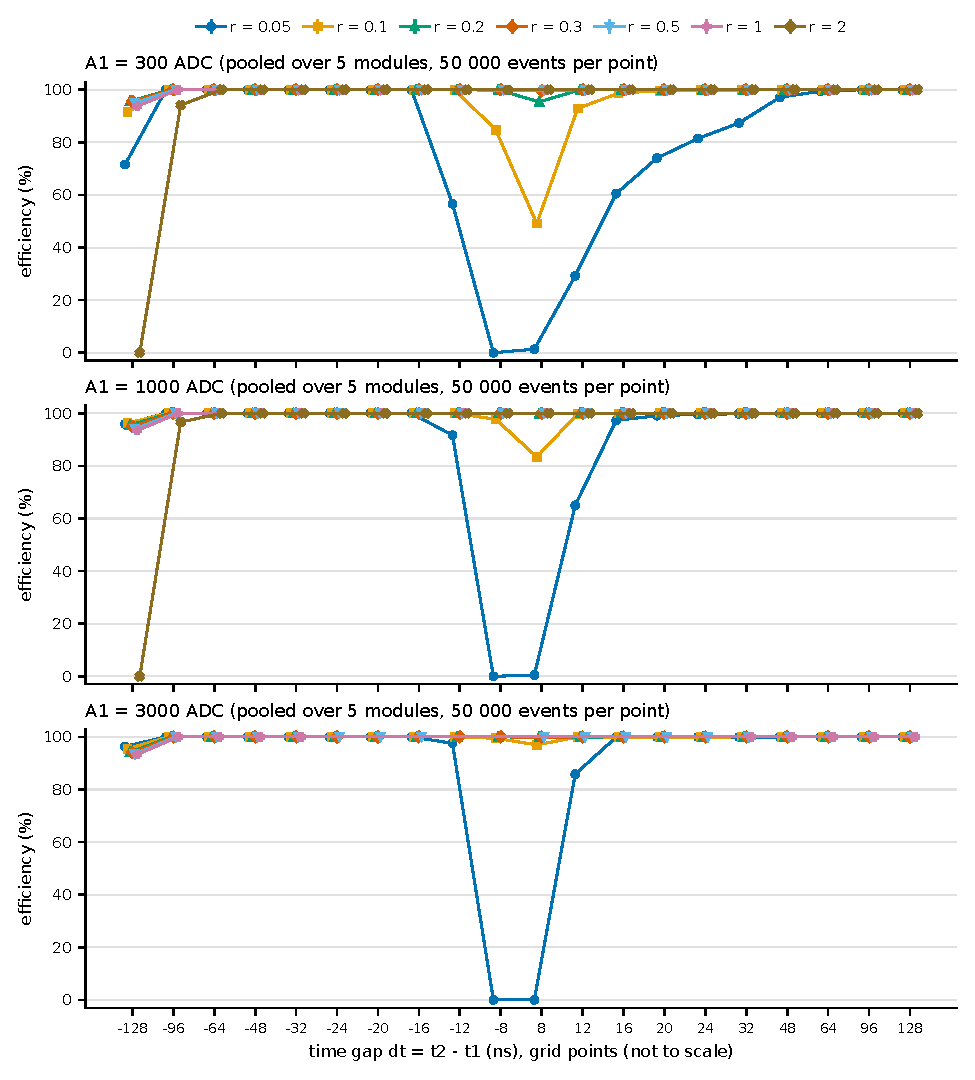
\includegraphics[width=\textwidth]{deconv_efficiency_vs_dt.pdf}
\caption{Efficiency (\%) to find the secondary pulse versus $\Delta t$, one line per $\rho$, for $A_1 = 300$, 1000 and 3000\,ADC (left to right). Each point pools the five modules (50\,000 events); the binomial errors are smaller than the markers. The $\Delta t$ values are drawn at equal spacing, so the horizontal axis is not to scale. The combinations dropped by the generator at $A_1 = 3000\adc$ are absent.}
\label{fig:deconv_eff}
\end{figure}

\begin{figure}[htbp]
\centering
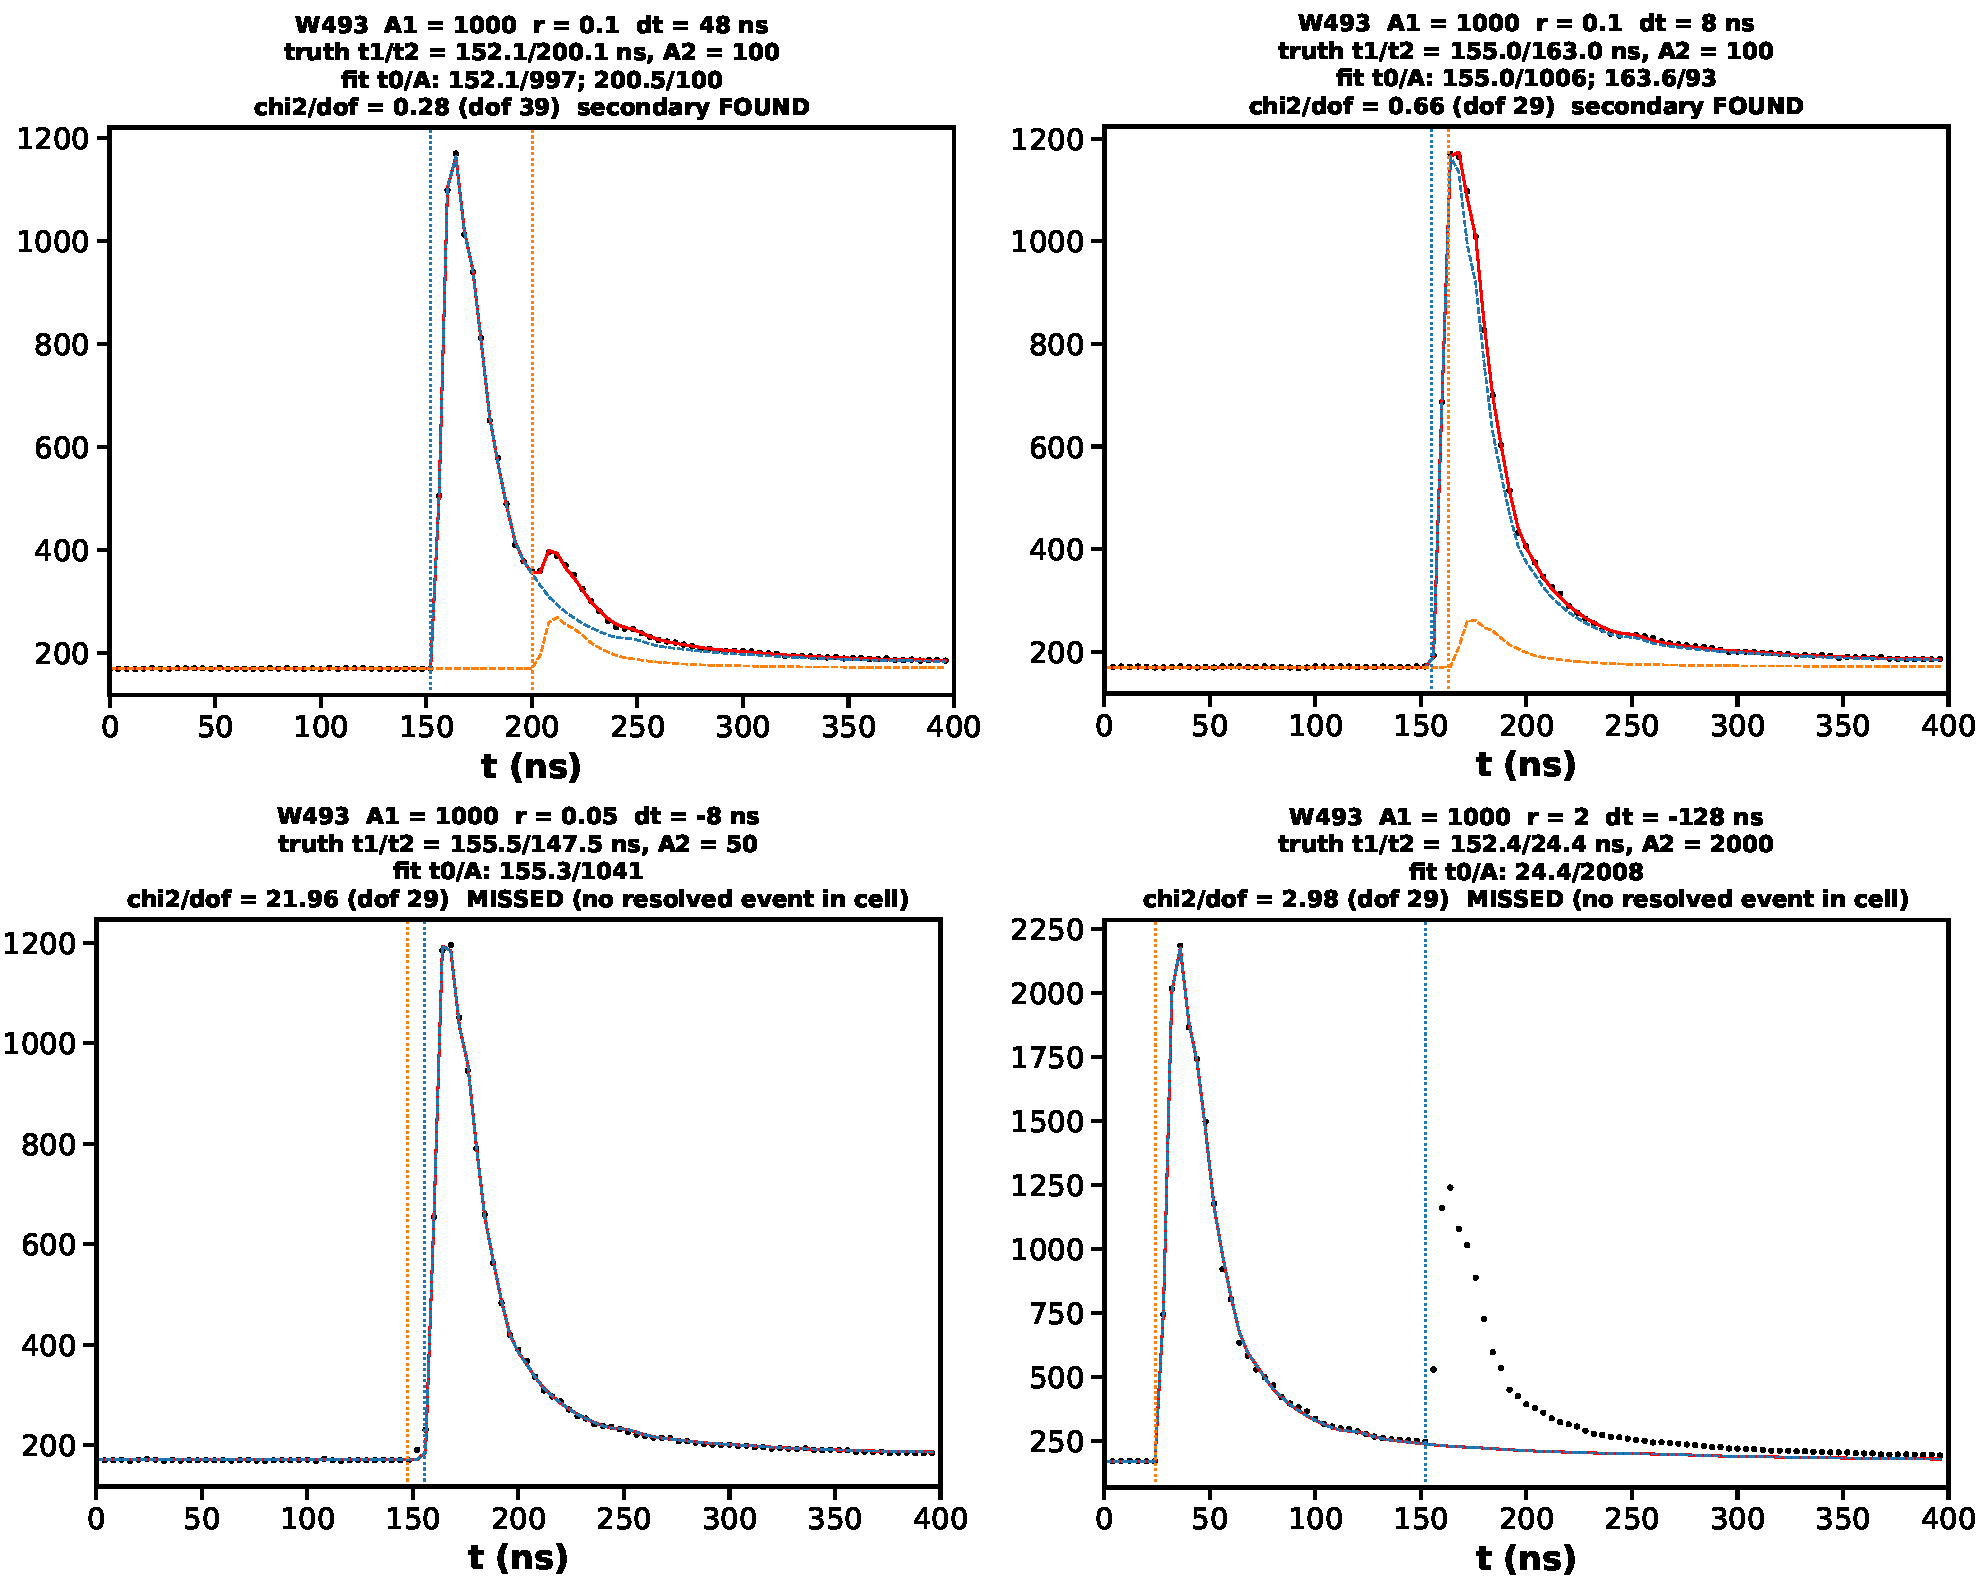
\includegraphics[width=\textwidth]{deconv_examples.pdf}
\caption{Fits of four generated events of W493 at $A_1 = 1000\adc$. Top left: $\rho = 0.1$, $\Delta t = +48\ns$, found. Top right: $\rho = 0.1$, $\Delta t = +8\ns$, found (cell efficiency 83.7\,\%). Bottom left: $\rho = 0.05$, $\Delta t = -8\ns$, missed; one pulse is fitted with $\chi^2/\mathrm{dof} = 22.0$ (cell efficiency 0\,\%). Bottom right: $\rho = 2$, $\Delta t = -128\ns$, missed; only the early pulse of 2000\,ADC is fitted (cell efficiency 0\,\%). Black dots: samples, pedestal included; red line: fitted model; dashed lines: fitted pulses in time order (blue, orange); dotted vertical lines: true onsets $t_1$ (blue) and $t_2$ (orange). The true pulse shapes are not drawn. Each panel is the first found event of its cell or, in a cell without one, its first event. Horizontal axis: time (ns); vertical axis: ADC.}
\label{fig:deconv_examples}
\end{figure}

\begin{figure}[htbp]
\centering
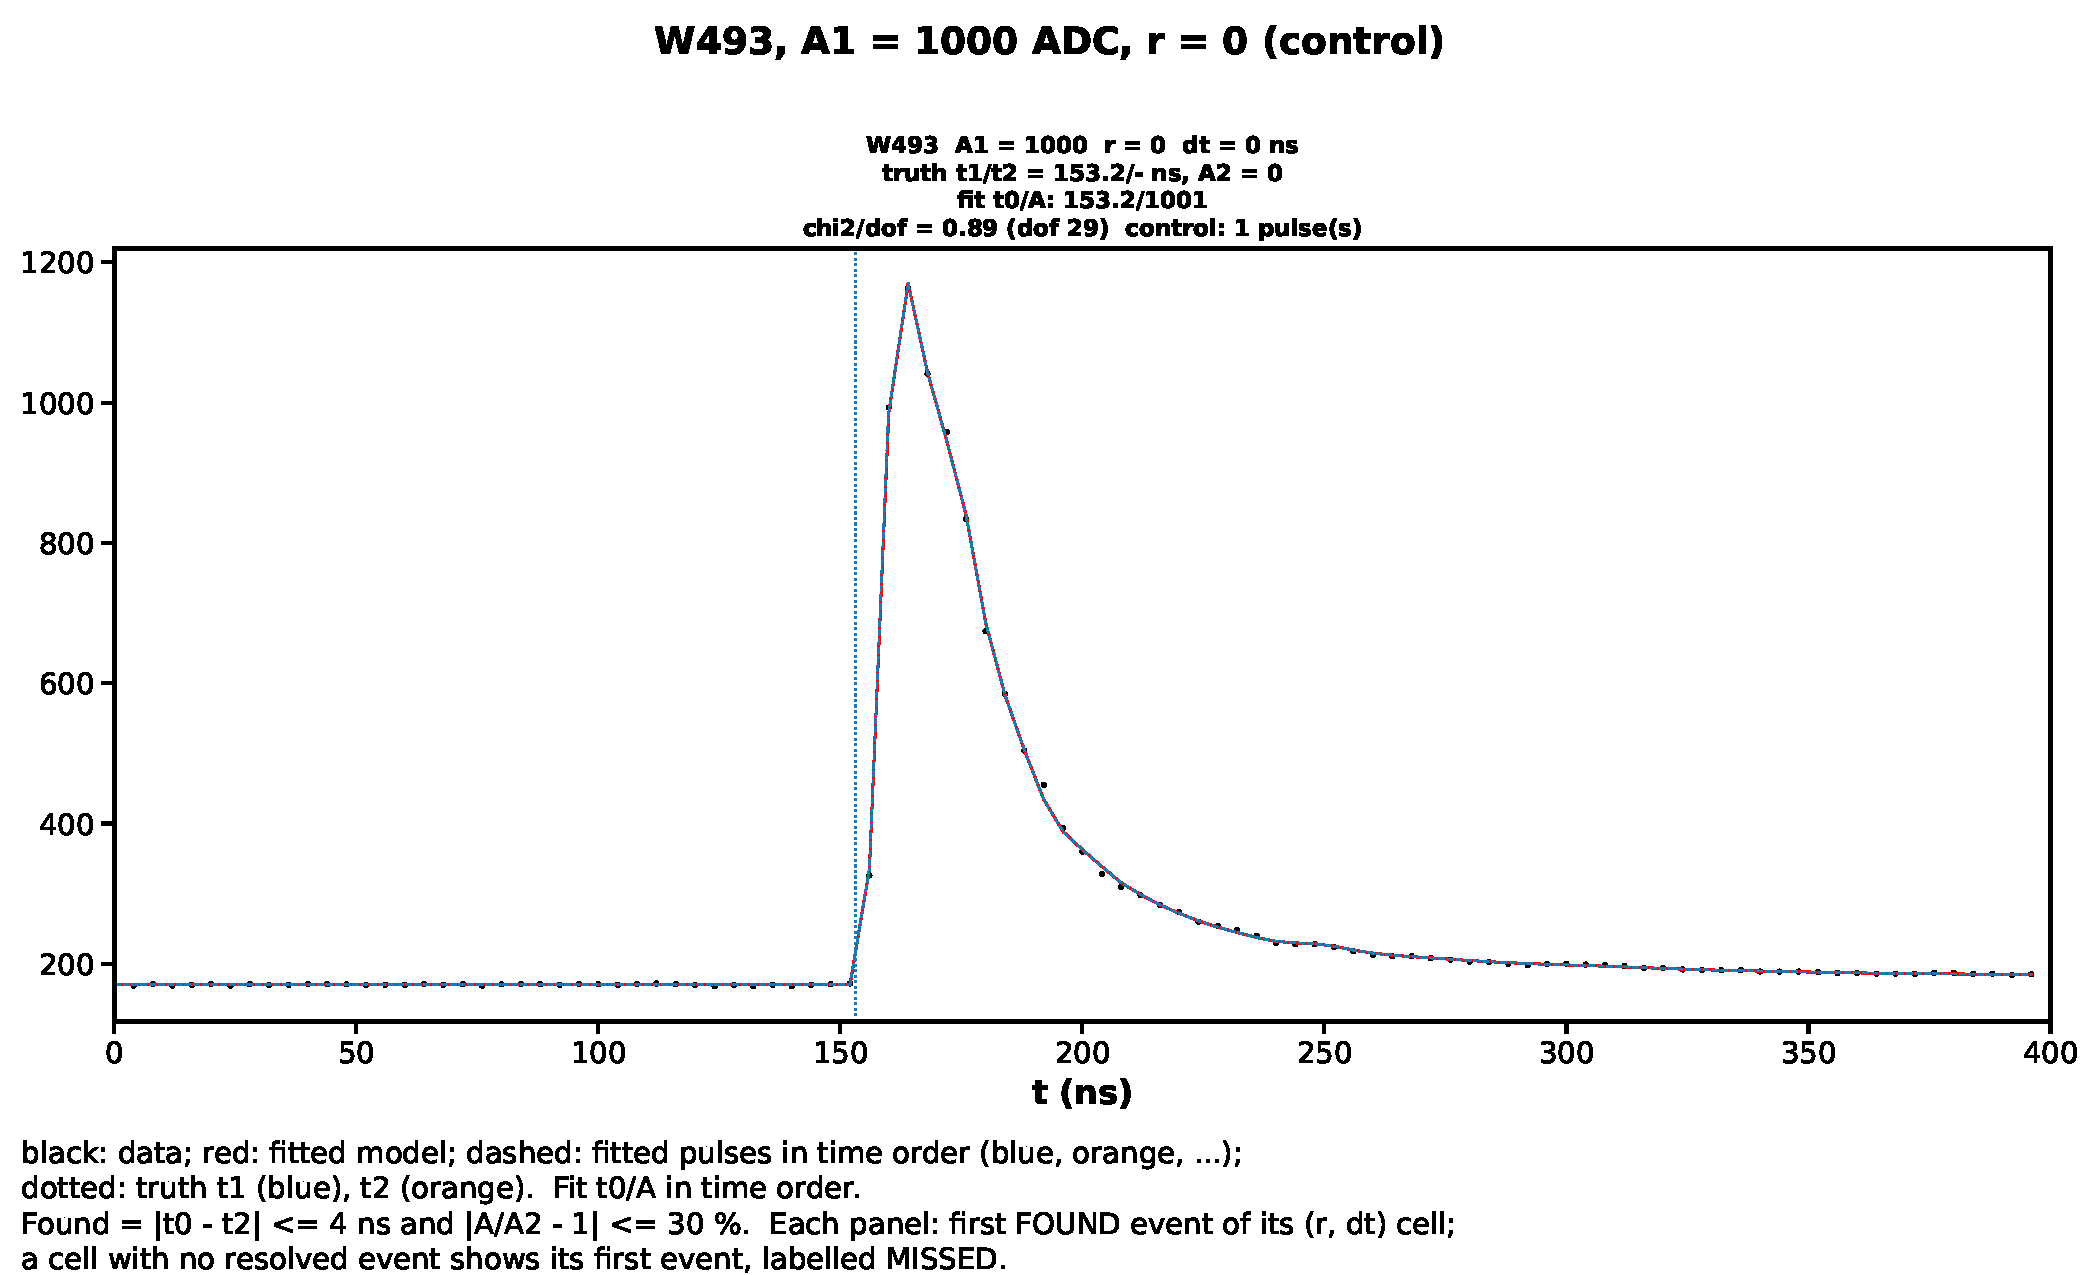
\includegraphics[width=0.6\textwidth]{deconv_example_control.pdf}
\caption{Fit of a control event of W493 at $A_1 = 1000\adc$, drawn as in Fig.~\ref{fig:deconv_examples}. The true onset is 153.2\,ns; the fit returns one pulse at 153.2\,ns with 1001\,ADC and $\chi^2/\mathrm{dof} = 0.89$ (29 degrees of freedom).}
\label{fig:deconv_control}
\end{figure}

\paragraph{False positives.} Of the 150\,000 control events 27 are fitted with two or more pulses (0.018\,\%). All 27 occur at $A_1 = 300\adc$ ($27/50\,000 = 0.054\,\%$; 8, 3, 0, 8 and 8 events in W493, W564, W664, W593 and W494); no control at 1000 or 3000\,ADC has a second pulse.

\paragraph{Main-pulse amplitude.} In the controls the median pull is at most $2.5 \times 10^{-4}$ in magnitude in every cell, and its width is 0.99 to 1.08\,\% at $A_1 = 300\adc$, 0.52 to 0.55\,\% at 1000\,ADC and 0.29 to 0.31\,\% at 3000\,ADC. Figure~\ref{fig:deconv_pull} shows the pull with a second pulse. A resolved secondary pulse at $|\Delta t| \ge 48\ns$ leaves the width at the control value, except for $\rho \ge 1$ at $\Delta t \le -48\ns$ (up to 1.47 times the control width). Towards small $|\Delta t|$ the width grows: for W493 at $\rho = 0.2$ and $\Delta t = +8\ns$ it is 2.68, 1.48 and 0.85\,\% at the three amplitudes, with medians between $-0.12$ and $0.00\,\%$. The largest W493 width, 4.63\,\% at $A_1 = 300\adc$, belongs to $\rho = 2$ at $\Delta t = -8\ns$. At $\rho = 1$ and $\Delta t = \pm 24\ns$ the W493 median shifts by $-0.2$ to $-0.6\,\%$; the cause is not determined.

\begin{figure}[htbp]
\centering
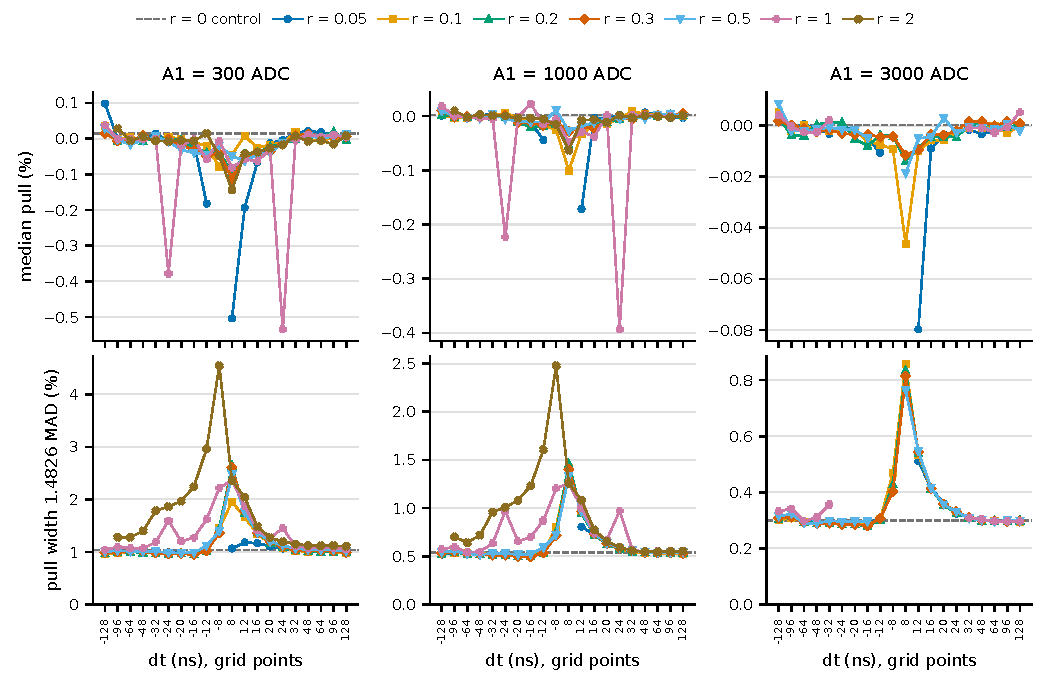
\includegraphics[width=\textwidth]{deconv_main_pull_vs_dt.pdf}
\caption{Main-pulse pull $\hat A_{\mathrm{main}}/A_1 - 1$ of the found events versus $\Delta t$, one line per $\rho$, for $A_1 = 300$, 1000 and 3000\,ADC (left to right). Top row: median (\%); bottom row: 1.4826 times the MAD (\%). Each point is the mean over the modules of the cell values of \code{efficiency.tsv}, using cells with at least 100 found events. The dashed grey line is the mean of the control cells.}
\label{fig:deconv_pull}
\end{figure}

\paragraph{Secondary pulse.} For W493 at $\rho = 0.1$ and $\Delta t = +128\ns$ the timing residual has a width of 0.21, 0.09 and 0.05\,ns and the amplitude residual a width of 3.2, 1.6 and 0.8\,\% at $A_1 = 300$, 1000 and 3000\,ADC, both without a shift. At $\Delta t = +8\ns$ the widths rise to 1.21, 0.73 and 0.43\,ns and to 23.7, 14.9 and 8.4\,\%, and the amplitude is high by 6.0, 1.7 and 0.4\,\% in the median. At $\rho = 0.05$ and $\Delta t = +12\ns$ the median amplitude excess is 22.4, 7.1 and 2.2\,\%. These statistics use the events inside the timing tolerance, which selects upward fluctuations of a small secondary pulse.

\paragraph{Failures at the edges of the grid.} At $\rho = 2$ and $\Delta t = -128\ns$ the efficiency is zero in all ten cells: the early pulse of twice the primary amplitude lies inside the first 30 samples, and the fit returns it alone (Fig.~\ref{fig:deconv_examples}, bottom right). The mechanism has not been traced in the code. For the other ratios the efficiency at $-128\ns$, pooled over the amplitudes, is 87.9 to 95.1\,\%, and for $\rho = 2$ at $-96\ns$ it is 95.4\,\%. A merged pair leaves a large $\chi^2/\mathrm{dof}$: its median at $\rho = 0.05$ and $\Delta t = -8\ns$ is 4.8, 47 and 426 at the three amplitudes. W494 has the lowest efficiency in every hard cell (65.8\,\% against 83.7 to 89.5\,\% in the other modules at $\rho = 0.1$, $\Delta t = +8\ns$, $A_1 = 1000\adc$); the reason is not determined.

\paragraph{Limits of the study.} The pull and the residuals leave out the events in which the secondary pulse was not found. The efficiency of finding the main pulse and its timing residual are not computed. Its results apply to five ring-2 modules, white noise and the 2.24\,GeV templates.
\clearpage

\section{Exotic waveforms}
\label{sec:exotic}

\paragraph{Purpose, inputs, outputs.} The exotic-waveform study flags the kept channels whose waveform is not a sum of template pulses, counts them per run type, module and cluster role, and measures what they cost in the elastic yields. Its inputs are the kept channels of the pile-up scan of Section~\ref{sec:rates} with the option \code{PILEUP\_EXOTIC=1} on the runs of Table~\ref{tab:runs} (99 raw-data files, the full scan), a two-file sample per run for the quantities the scan does not store, and the gated clusters of the calibration chain of Section~\ref{sec:calib} (control~v3). Run 24937 (\code{3p49GeV\_H2}) is not a good run and is excluded; only PbWO$_4$ modules enter. The outputs are the tables and figures of the steps P1 to P13 in \code{pileup\_analysis/exotic\_events/} and the consolidated \code{exotic\_summary\_20261118.pdf}, whose front matter holds the numbers quoted here. The flags are markers only: no channel is masked or corrected, and a policy that drops every flagged channel was tested and is not adopted (Section~\ref{sec:exotic_status}).

\subsection{Types and identification}
\label{sec:exotic_id}

Twelve waveforms picked by eye from the scans define four types (Fig.~\ref{fig:exotic_types}): a tail below the baseline after the pulse (type~1), an anomalously wide smooth pulse (type~2), a smooth wide pulse that the fitter describes as close pile-up (type~3), and a clipped pulse with secondary pulses at the clipped samples (type~4). Each type gets a flag built from quantities of the fitted waveform (Table~\ref{tab:exotic_flags}); a fifth flag separates the lone saturated pulses from type~4.

\begin{figure}[htbp]
\centering
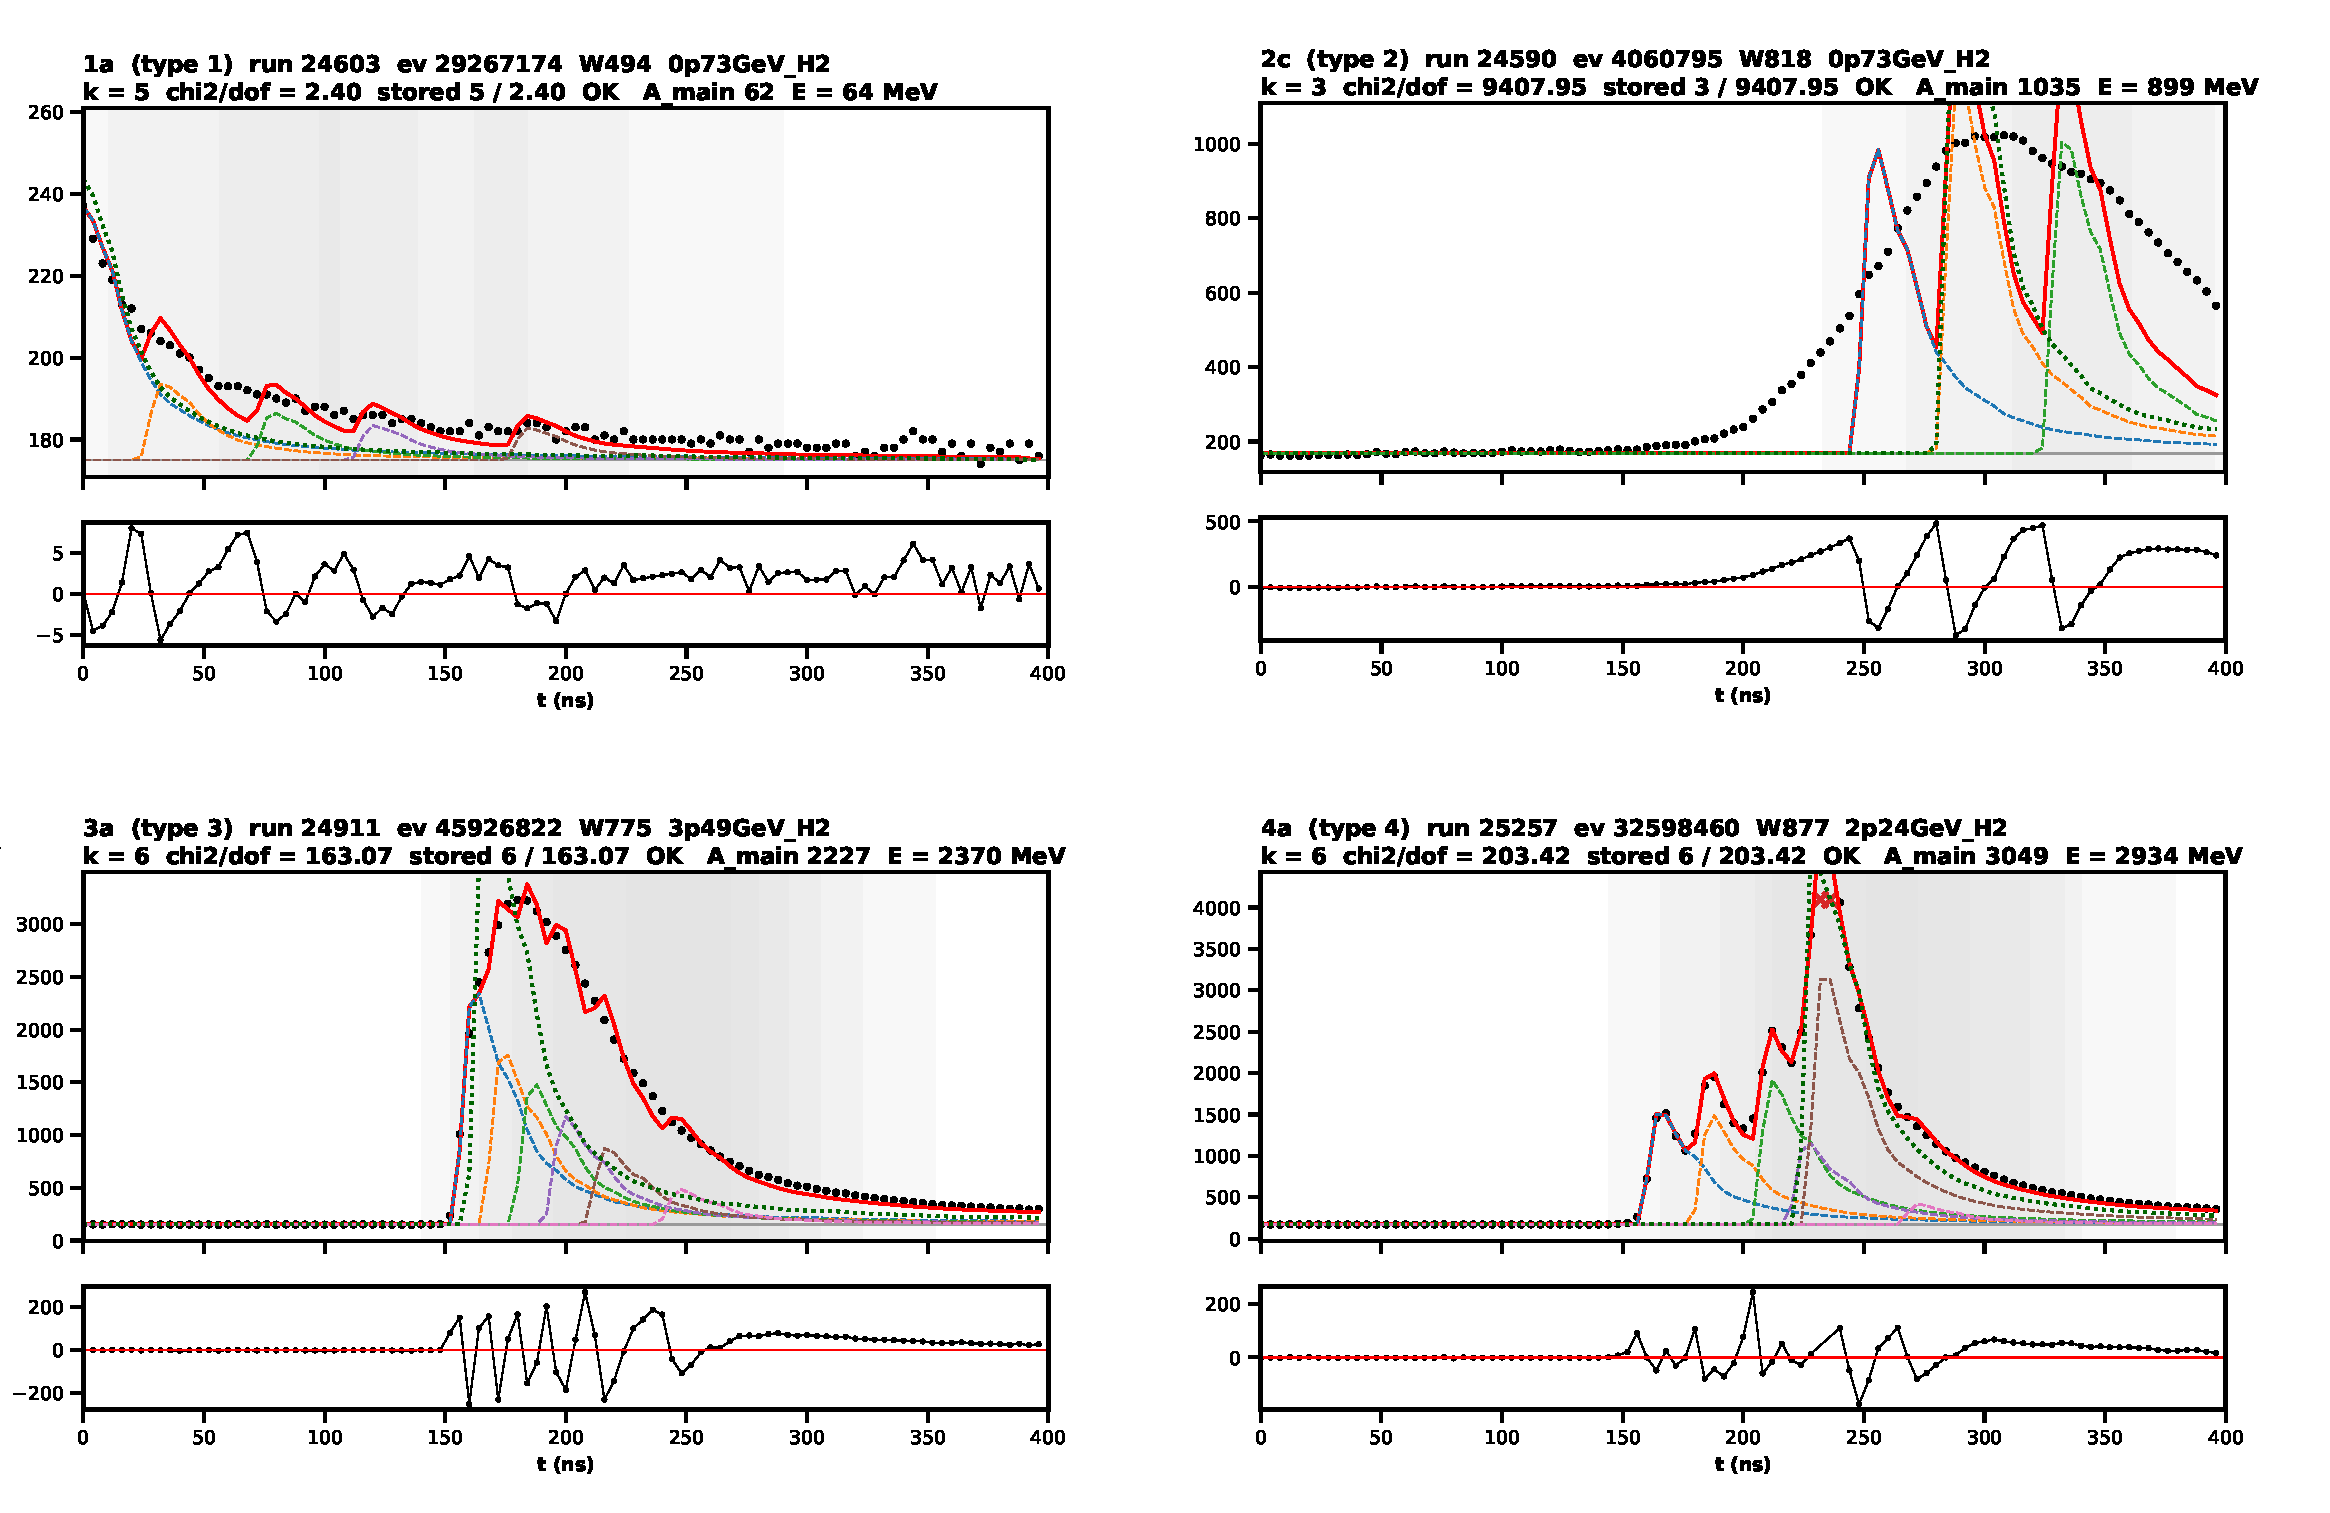
\includegraphics[width=\textwidth]{exotic_types_examples.pdf}
\caption{One of the twelve user examples per type, refitted from the raw data (step P1): type~1, W494 in run 24603; type~2, W818 in run 24590; type~3, W775 in run 24911; type~4, W877 in run 25257. Black dots: raw samples; red line: total fit; dashed lines: fitted pulses in time order; dotted green: single-pulse refit; shaded: fit windows. Lower strips: data minus fit. Horizontal axis: time after the start of the readout (ns); vertical axis: ADC. Each title gives the module, run, event, $K$, $\chi^2/\mathrm{dof}$, $A_{\mathrm{main}}$ and $E_{\mathrm{main}}$.}
\label{fig:exotic_types}
\end{figure}

\subsubsection{Procedure}

\begin{enumerate}
\item \textbf{Quantities.} For each kept channel the scan computes the baseline step $\delta b$, the first-30-sample baseline minus the reference baseline $p_{\mathrm{ref}}$ of the module, and the tail level, the mean of the pulse-free samples among the last 10 minus the first-30-sample baseline, both in units of $\sigma_{\mathrm{ref}}$. The tail level is undefined when fewer than 8 of the last 10 samples are pulse-free. The width ratio $w_{50}$ is the full width at half maximum of the data divided by that of the template, and $\chi^2_{\mathrm{stretch}}$ the $\chi^2$ of a refit with a single template stretched in time. The scan also records the number of clipped samples, the distance of the nearest secondary onset to the clipped stretch, and the energy $E_{\mathrm{sec}}$ of the largest secondary pulse.
\item \textbf{Flags.} The five flags of Table~\ref{tab:exotic_flags} use one set of thresholds for all run types. The template FWHM is 23.5\,ns for PbWO$_4$ in every run type, so $w_{50} > 3$ means a data FWHM above 70\,ns. Thresholds set per run type from the median and width of the $K = 1$ core move little (only the tantalum $\delta b$ threshold, 8 to 9.76) and are kept as a reference set in the step P4 output.
\item \textbf{Exclusions for f2.} A clipped record (one or more clipped samples) is never f2, and neither is a window-truncated pulse, $t_0 > 284\ns$, whose width cannot be measured. The truncation rule removes 23 to 25\,\% of the hydrogen f2 flags and 0.6\,\% of the tantalum ones; the clip rule removes 0, 13, 9 and 0 flags (0.73, 2.24, 3.49\,GeV H$_2$, Ta).
\item \textbf{Exclusive categories.} Each channel counts once, in the first category of the order f4, f5, f1, f2, f3 that it satisfies. Saturated records come first so that a clipped pulse is never counted as wide or as a tail. f1 precedes f2 and f3 because the tantalum tail population satisfies all three: with f1 first, the tantalum f2 rate falls from 0.111 to 0.016\,\% and the f3 rate from 0.392 to 0.197\,\%.
\item \textbf{Samples.} The full scan stores only the candidate rows of the hydrogen files, so amplitudes, $w_{50}$ distributions and the cluster-level join use the two-file sample per run for hydrogen and the stored full-scan files for tantalum, 5 to 61 million kept channels per run type.
\end{enumerate}

\begin{table}[htbp]
\centering
\caption{Exotic flags, evaluated in the order of the exclusive priority f4 $>$ f5 $>$ f1 $>$ f2 $>$ f3. $\delta b$ and the tail level are in units of $\sigma_{\mathrm{ref}}$; $n_{\mathrm{clip}}$ is the number of clipped samples; $n_m$ the number of fitted samples; $\Lambda = 2$.}
\label{tab:exotic_flags}
\small
\begin{tabular}{llp{0.58\textwidth}}
\toprule
Flag & Type & Condition \\
\midrule
f4 & 4, clipped with secondary & $n_{\mathrm{clip}} \ge 1$ and (a secondary onset within 8\,ns of the clipped stretch, or $E_{\mathrm{sec}} > 0.5\,E_b$) \\
f5 & saturated, alone & $n_{\mathrm{clip}} \ge 1$ and not f4 \\
f1 & 1, tail below baseline & $\delta b > 8$ and tail $< -5$ \\
f2 & 2, wide & $w_{50} > 3$, $n_{\mathrm{clip}} = 0$, $t_0 \le 284\ns$ \\
f3 & 3, smooth-wide & $K \ge 2$ and $\chi^2_{\mathrm{stretch}} \le \chi^2_K + \Lambda\,(K - 1)\ln n_m$ \\
\bottomrule
\end{tabular}
\end{table}

\subsection{Rates and module maps}
\label{sec:exotic_rates}

Table~\ref{tab:exotic_rates} gives the exclusive rates of the full scan. The hydrogen run types flag 0.07 to 0.09\,\% of their kept channels, the tantalum run type 1.1\,\%, and f1 carries 81\,\% of the tantalum flags. Saturated records (f4 plus f5) are 0.0038\,\% of the kept channels at 2.24\,GeV H$_2$, 0.0015\,\% at 3.49\,GeV and below $2 \times 10^{-4}$\,\% in the other two run types. Among the pulses above $0.5\,E_b$ in the two-file sample the saturated share is 0.102\,\% at 2.24\,GeV H$_2$ ($880/864\,982$), 0.055\,\% at 3.49\,GeV, $5 \times 10^{-4}$\,\% at 0.73\,GeV (2 pulses) and 0.003\,\% in tantalum. Saturation is up to 0.1\,\% of the full-energy pulses for now; the sample statistics are too small for a firmer number, and f5 is kept for the full-data scan on the farm.

\begin{table}[htbp]
\centering
\caption{Exclusive category rates of the full scan, in \% of the kept PbWO$_4$ channels (uniform thresholds, run 24937 excluded). $N_{\mathrm{kept}}$ in millions; the 68\,\% Wilson intervals are in \code{exotic\_P4\_module\_rates\_20261117\_summary.tsv}.}
\label{tab:exotic_rates}
\small
\begin{tabular}{lrrrrrrr}
\toprule
Run type & $N_{\mathrm{kept}}$ & f1 & f2 & f3 & f4 & f5 & any \\
\midrule
\code{0p73GeV\_H2}     & 20.95 & 0.0322 & 0.0011 & 0.0359 & 0.00011 & 0.00004 & 0.0693 \\
\code{2p24GeV\_H2}     & 95.80 & 0.0595 & 0.0005 & 0.0259 & 0.0024  & 0.0015  & 0.0896 \\
\code{3p49GeV\_H2}     & 46.06 & 0.0560 & 0.0003 & 0.0154 & 0.0008  & 0.0007  & 0.0733 \\
\code{2p24GeV\_Ta\_X17} & 79.22 & 0.9005 & 0.0164 & 0.1975 & 0.00002 & 0.00001 & 1.1143 \\
\bottomrule
\end{tabular}
\end{table}

\paragraph{Module maps.} Figure~\ref{fig:exotic_maps} shows the module rates of f1, f3 and the saturated records for hydrogen and tantalum at 2.24\,GeV. In tantalum f1 and f2 concentrate in the inner ring around the beam hole and fall with radius (f1 from 1.03\,\% at 0 to 120\,mm to 0.17\,\% at 320 to 450\,mm); f3 is U-shaped, lowest at mid radius. In hydrogen f3 rises toward the outer edge at all three energies, and at 2.24 and 3.49\,GeV so do the saturated records (2.24\,GeV: 0.001\,\% at 0 to 120\,mm, 0.039\,\% at 320 to 450\,mm), so saturation is not an inner-ring effect. The modules of highest rate (at least 100 kept channels and 5 flags) are W335 at 0.73\,GeV (f3 $267/2877 = 9.3\,\%$), the ringing module of Section~\ref{sec:rates}, and W613 for the saturated records at 2.24 and 3.49\,GeV (f4 2.1 and 3.1\,\%), followed by W307. No module is masked: the flags stay per channel.

\begin{figure}[htbp]
\centering
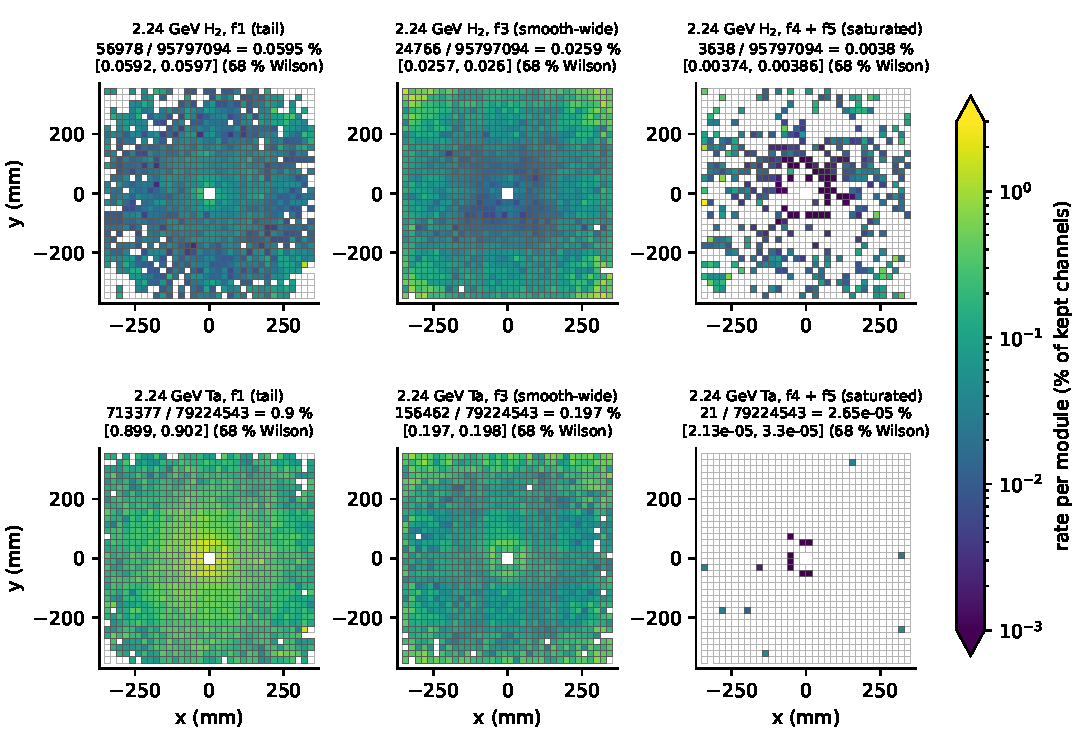
\includegraphics[width=\textwidth]{exotic_module_maps.pdf}
\caption{Exclusive category rate per PbWO$_4$ module for f1, f3 and the saturated records (f4 plus f5) in \code{2p24GeV\_H2} (top) and \code{2p24GeV\_Ta\_X17} (bottom), full scan, one logarithmic colour scale from 0.001 to 3\,\%. White: no flag; light grey: fewer than 30 kept channels. Each title gives the flagged and kept channels of the run type. Axes: module position $x$, $y$ (mm).}
\label{fig:exotic_maps}
\end{figure}

\paragraph{Rates per energy slice.} Table~\ref{tab:exotic_slices} and Fig.~\ref{fig:exotic_slices} give the exclusive rates per slice of the channel energy ($A_{\mathrm{main}}$ times the gain, channels of at least 10\,MeV) for the 2.24\,GeV hydrogen and tantalum run types; the step P12 output holds the same tables for 0.73 and 3.49\,GeV. The flags concentrate between 50 and 300\,MeV: the hydrogen any-flag rate is 0.26 to 0.27\,\% at 2.24\,GeV, 0.23 to 0.24\,\% at 3.49\,GeV and 0.18 to 0.33\,\% at 0.73\,GeV (intervals of $\pm 0.01$\,\% or less), carried by f1 at the two higher energies and by f3 at 0.73\,GeV ($0.220 \pm 0.006\,\%$ at 100 to 300\,MeV). Tantalum is about ten times higher, $2.54 \pm 0.01\,\%$ at 100 to 300\,MeV, almost all f1. Between 1 and 2.5\,GeV the any-flag rates have fallen by a factor of 7 to 34 (0.008 to 0.024\,\% at 2.24\,GeV H$_2$, 0.007 to 0.034\,\% at 3.49\,GeV, 0.14 to 0.22\,\% in tantalum, with intervals of $\pm 0.007$\,\% or less), with f3 the largest category. Above the beam energy the rates at 2.24 and 3.49\,GeV rise to 39 to 100\,\% ($\pm 7$\,\% or less, fewer than 15 channels per slice at 0.73\,GeV) and are mostly f4 and f5 (f3 $5.3^{+0.9}_{-0.8}\,\%$ at 2.5 to 3.5\,GeV). A fit extrapolated over clipped samples places the pulse above $E_b$ by construction, so these slices count the saturated records and measure no rate.

At cluster level (dashed curves, per slice of $E_{\mathrm{cluster}}$) the fraction of clusters with a flagged member is flat in hydrogen below the beam energy, 0.11 to 0.54\,\% (intervals 0.108 to 0.118 and 0.511 to 0.567\,\%, slices of at least $10^4$ clusters), and rises in tantalum from $1.26 \pm 0.06\,\%$ at 10 to 50\,MeV to $7.02 \pm 0.03\,\%$ at 1000 to 1500\,MeV. Below the beam energy the flagged members carry a mean fraction $\langle f_E \rangle$ per cluster of 0.029 to 0.29\,\% in hydrogen (same slices) and 0.49 to 0.74\,\% in tantalum below 2.5\,GeV ($\pm 0.04$\,\% or less), and 34 to 68\,\% ($\pm 4$\,\% or less) for the 2.24\,GeV hydrogen clusters at or above 2.5\,GeV, the saturated fakes of Section~\ref{sec:exotic_cluster}.

\begin{table}[htbp]
\centering
\caption{Exclusive category rate per slice of the channel energy (MeV), in \% of the kept PbWO$_4$ channels of the slice with the asymmetric 68\,\% Wilson interval; $N$ in millions (counts below 10\,000 as given). A cell $<x$ holds no flag and gives the upper end of the interval, rounded up. Hydrogen from the two-file sample, tantalum from the 19 stored full-scan files. Source: \code{exotic\_P12\_rates\_vs\_energy\_20261118.tsv}, table \code{chan}.}
\label{tab:exotic_slices}
\scriptsize
\setlength{\tabcolsep}{3.5pt}
\begin{tabular}{lrllllll}
\toprule
Slice & $N$ & f1 & f2 & f3 & f4 & f5 & any \\
\midrule
\multicolumn{8}{l}{\code{2p24GeV\_H2}} \\
10--50 & 14.69 & $0.0131^{+0.0003}_{-0.0003}$ & $0.0004^{+0.0001}_{-0.0000}$ & $0.0114^{+0.0003}_{-0.0003}$ & $<7{\cdot}10^{-6}$ & $<7{\cdot}10^{-6}$ & $0.0249^{+0.0004}_{-0.0004}$ \\
50--100 & 2.66 & $0.2455^{+0.0031}_{-0.0030}$ & $0.0004^{+0.0001}_{-0.0001}$ & $0.0166^{+0.0008}_{-0.0008}$ & $<4{\cdot}10^{-5}$ & $<4{\cdot}10^{-5}$ & $0.2626^{+0.0032}_{-0.0031}$ \\
100--300 & 2.37 & $0.2033^{+0.0030}_{-0.0029}$ & $0.0002^{+0.0001}_{-0.0001}$ & $0.0667^{+0.0017}_{-0.0017}$ & $<5{\cdot}10^{-5}$ & $<5{\cdot}10^{-5}$ & $0.2702^{+0.0034}_{-0.0034}$ \\
300--500 & 0.69 & $0.0029^{+0.0007}_{-0.0006}$ & $0.0006^{+0.0004}_{-0.0002}$ & $0.1313^{+0.0044}_{-0.0043}$ & $<2{\cdot}10^{-4}$ & $<2{\cdot}10^{-4}$ & $0.1348^{+0.0045}_{-0.0043}$ \\
500--1000 & 0.77 & $0.0012^{+0.0005}_{-0.0003}$ & $0.0023^{+0.0006}_{-0.0005}$ & $0.0846^{+0.0034}_{-0.0032}$ & $<2{\cdot}10^{-4}$ & $0.0001^{+0.0002}_{-0.0001}$ & $0.0882^{+0.0034}_{-0.0033}$ \\
1000--1500 & 0.61 & $<2{\cdot}10^{-4}$ & $0.0007^{+0.0004}_{-0.0003}$ & $0.0069^{+0.0012}_{-0.0010}$ & $<2{\cdot}10^{-4}$ & $0.0003^{+0.0003}_{-0.0002}$ & $0.0079^{+0.0012}_{-0.0011}$ \\
1500--2500 & 0.39 & $<3{\cdot}10^{-4}$ & $0.0018^{+0.0008}_{-0.0006}$ & $0.0140^{+0.0020}_{-0.0018}$ & $0.0082^{+0.0016}_{-0.0013}$ & $<3{\cdot}10^{-4}$ & $0.0240^{+0.0026}_{-0.0024}$ \\
2500--3500 & 681 & $<0.2$ & $0.29^{+0.29}_{-0.15}$ & $5.29^{+0.92}_{-0.79}$ & $25.8^{+1.7}_{-1.6}$ & $7.8^{+1.1}_{-1.0}$ & $39.2^{+1.9}_{-1.9}$ \\
3500--4000 & 181 & $<0.6$ & $0.55^{+0.88}_{-0.34}$ & $1.7^{+1.2}_{-0.7}$ & $38.1^{+3.7}_{-3.5}$ & $33.7^{+3.6}_{-3.4}$ & $74.0^{+3.1}_{-3.4}$ \\
$>$4000 & 491 & $<0.3$ & $<0.3$ & $<0.3$ & $54.2^{+2.2}_{-2.3}$ & $45.4^{+2.3}_{-2.2}$ & $99.59^{+0.20}_{-0.41}$ \\
\midrule
\multicolumn{8}{l}{\code{2p24GeV\_Ta\_X17}} \\
10--50 & 38.58 & $0.5875^{+0.0012}_{-0.0012}$ & $0.0273^{+0.0003}_{-0.0003}$ & $0.2342^{+0.0008}_{-0.0008}$ & $<3{\cdot}10^{-6}$ & $<3{\cdot}10^{-6}$ & $0.8490^{+0.0015}_{-0.0015}$ \\
50--100 & 8.73 & $2.0012^{+0.0048}_{-0.0047}$ & $0.0048^{+0.0002}_{-0.0002}$ & $0.1294^{+0.0012}_{-0.0012}$ & $<2{\cdot}10^{-5}$ & $<2{\cdot}10^{-5}$ & $2.1354^{+0.0049}_{-0.0049}$ \\
100--300 & 6.25 & $2.3668^{+0.0061}_{-0.0061}$ & $0.0004^{+0.0001}_{-0.0001}$ & $0.1719^{+0.0017}_{-0.0016}$ & $<2{\cdot}10^{-5}$ & $<2{\cdot}10^{-5}$ & $2.5391^{+0.0063}_{-0.0063}$ \\
300--500 & 1.42 & $0.4059^{+0.0054}_{-0.0053}$ & $0.0004^{+0.0002}_{-0.0001}$ & $0.2801^{+0.0045}_{-0.0044}$ & $<8{\cdot}10^{-5}$ & $<8{\cdot}10^{-5}$ & $0.6863^{+0.0070}_{-0.0069}$ \\
500--1000 & 1.23 & $0.1675^{+0.0037}_{-0.0036}$ & $0.0001^{+0.0001}_{-0.0001}$ & $0.2500^{+0.0045}_{-0.0045}$ & $<9{\cdot}10^{-5}$ & $<9{\cdot}10^{-5}$ & $0.4176^{+0.0058}_{-0.0058}$ \\
1000--1500 & 0.46 & $0.0613^{+0.0038}_{-0.0036}$ & $<3{\cdot}10^{-4}$ & $0.1623^{+0.0061}_{-0.0058}$ & $<3{\cdot}10^{-4}$ & $<3{\cdot}10^{-4}$ & $0.2236^{+0.0071}_{-0.0069}$ \\
1500--2500 & 0.31 & $0.0319^{+0.0034}_{-0.0031}$ & $<4{\cdot}10^{-4}$ & $0.1068^{+0.0060}_{-0.0057}$ & $0.0026^{+0.0011}_{-0.0008}$ & $<4{\cdot}10^{-4}$ & $0.1413^{+0.0069}_{-0.0066}$ \\
2500--3500 & 46 & $<3$ & $<3$ & $4.3^{+4.1}_{-2.2}$ & $2.2^{+3.4}_{-1.3}$ & $10.9^{+5.4}_{-3.8}$ & $17.4^{+6.3}_{-4.9}$ \\
3500--4000 & 5 & $<20$ & $<20$ & $<20$ & $<20$ & $<20$ & $<20$ \\
$>$4000 & 6 & $<20$ & $<20$ & $<20$ & $67^{+16}_{-20}$ & $33^{+20}_{-16}$ & $100^{+0}_{-14}$ \\
\bottomrule
\end{tabular}
\end{table}

\begin{figure}[htbp]
\centering
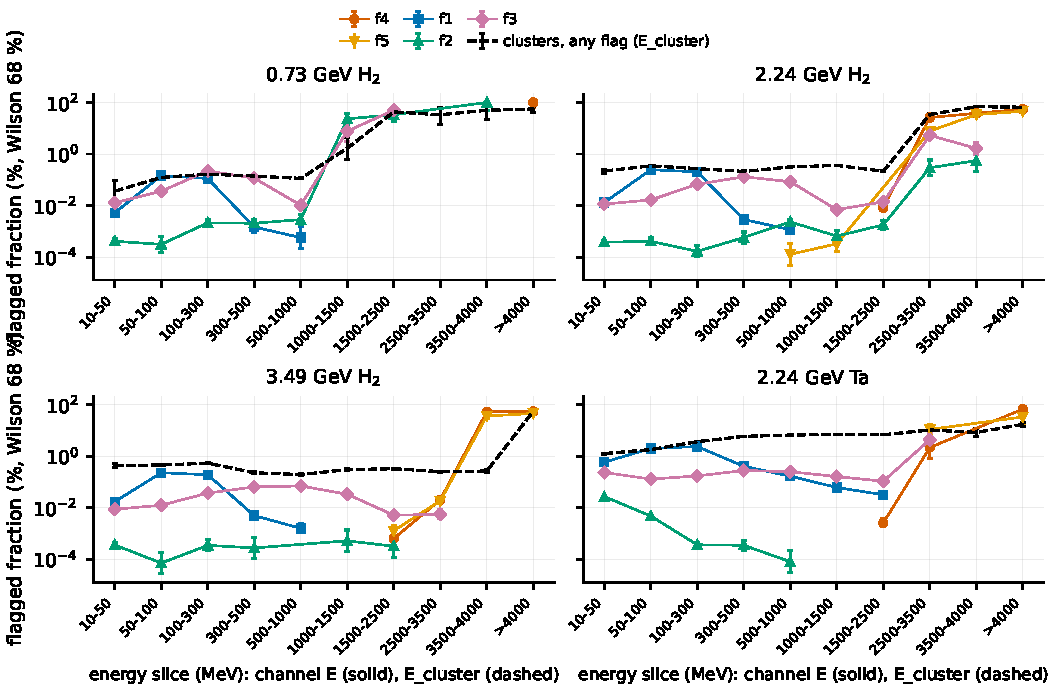
\includegraphics[width=0.8\textwidth]{exotic_rates_vs_energy.pdf}
\caption{Exclusive category rate per slice of the channel energy for the four run types (solid, one curve per flag, 68\,\% Wilson error bars; slices with no flag omitted) and the fraction of clusters with a flagged member per slice of the cluster energy (dashed). Source: \code{exotic\_P12\_rates\_vs\_energy\_20261118.tsv}.}
\label{fig:exotic_slices}
\end{figure}

\subsection{Nature of the categories}
\label{sec:exotic_nature}

\paragraph{f1: tails of earlier pulses.} The f1 channels are small: the median fitted $A_{\mathrm{main}}$ is 71 to 91\,ADC, 2 to 4\,\% of $E_b$ (12\,\% at 0.73\,GeV). In tantalum the inner-ring f1 rate follows the occupancy of the run: across 21 file splits of three runs it rises by $0.034 \pm 0.002\,\%$ per kept channel per event (elasticity 1.06). Run 26230 has 1.21 times the rate of run 25800 at 1.17 times its kept channels and current (3.5 against 3.0\,nA; the current of run 25800 is taken from the logbook, the run database has no entry). Current, occupancy, trigger version and the inner-layer high voltage change together between these runs and cannot be separated. The dependence is consistent with descending tails of earlier pulses, whose rate grows with the pulse rate. Of the 557\,506 tantalum f1 rows of the stored files, 366\,283 (66\,\%) lie outside any cluster, and 97.5\,\% of those have no hit of their own and a pulse before the hit window ($t < 100\ns$); they need no action for the yields.

\paragraph{f2: wide pulses.} Figure~\ref{fig:exotic_w50} shows the fitted amplitude against $w_{50}$. The hydrogen f2 channels are bimodal in amplitude. The high-amplitude mode, $A_{\mathrm{main}} > 300\adc$, holds 34 of 107 f2 channels at 2.24\,GeV, 31 of them fitted with $K \ge 4$ and spread over 18 modules: merged pile-up trains of four or more pulses. At 0.73\,GeV the mode is 25 of 48 channels, 19 of them on W335, and at 3.49\,GeV 3 of 35. The low-amplitude mode consists of noisy trains, also fitted with several pulses. The cut $w_{50} = 3$ sits in a density gap for hydrogen, where the counts fall by a factor 14 to 42 from the $w_{50}$ bin 2 to 3 to the bin 3 to 4. In tantalum f2 is not a distinct population: 8 of 11\,026 channels exceed 300\,ADC, the median fitted amplitude is 31\,ADC, 10\,603 of the 11\,018 low-amplitude channels have $K \ge 4$, and the counts fall by only 3.4 across the cut. The tantalum f2 channels are the tail of the baseline-wobble over-fit of the inner ring, and the cut is kept at 3 as a position in that tail.

\begin{figure}[htbp]
\centering
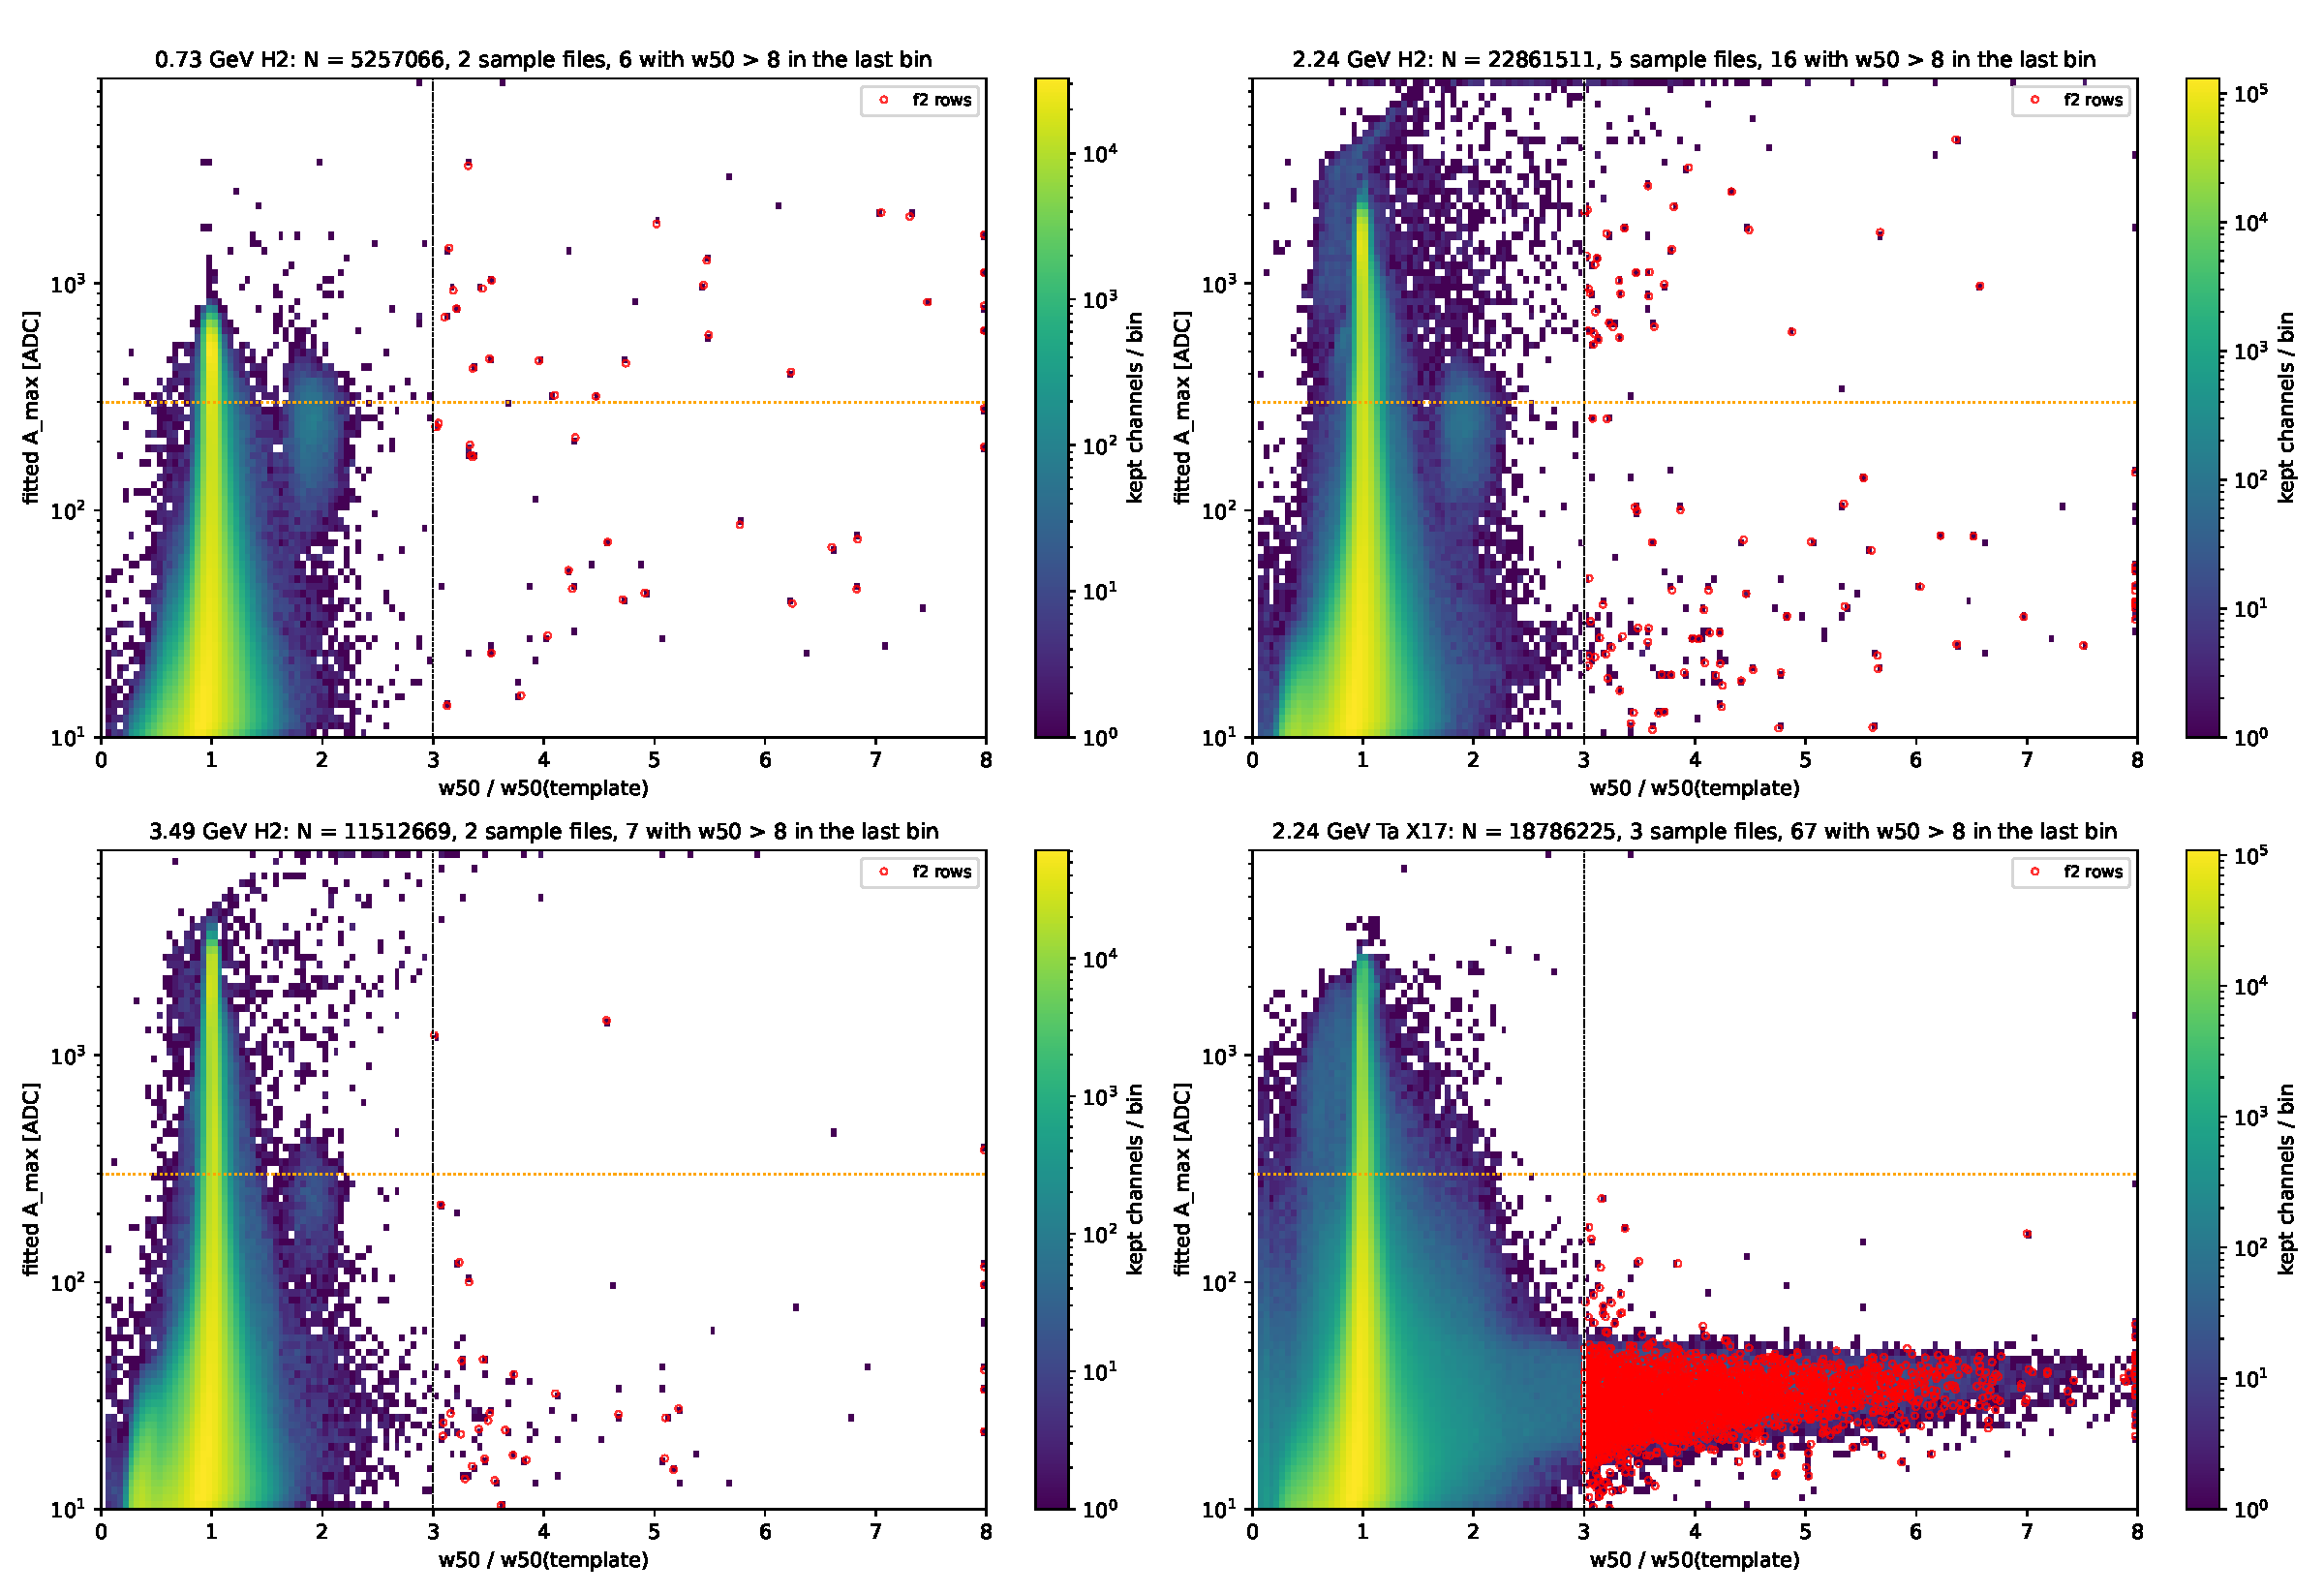
\includegraphics[width=\textwidth]{exotic_amp_vs_w50.pdf}
\caption{Fitted $A_{\mathrm{main}}$ against the width ratio $w_{50}$ for all kept PbWO$_4$ channels of the step P6 samples (file counts in the panel titles; the tantalum numbers in the text come from the full scan), one panel per run type, with the f2 channels circled in red (at most 3000 drawn). Dashed: the cut $w_{50} = 3$; dotted: $A_{\mathrm{main}} = 300\adc$. Colour: kept channels per bin, logarithmic.}
\label{fig:exotic_w50}
\end{figure}

\paragraph{f3: over-fit of a smooth wide pulse.} f3 marks a channel whose $K \ge 2$ fit is not better, by the BIC criterion of Table~\ref{tab:exotic_flags}, than a single stretched template. Its shape alone does not separate it from real close pile-up, which the stretched template describes equally well, so f3 marks an ambiguous shape and does not by itself identify a defect. Its amplitudes are broad in hydrogen (16th to 84th percentile 20 to 45 and 450 to 560\,ADC) and small in tantalum (median raw peak 19\,ADC).

\paragraph{f4 and f5: saturation.} The f4 and f5 channels have a raw peak at the clip level, about 3930\,ADC above the pedestal, and a median fitted amplitude of 1.1 to 2.0\,$E_b$ (the two 0.73\,GeV f4 channels lie far above). The join to clusters finds two populations of saturated seeds in the elastic window (Section~\ref{sec:exotic_cluster}): single-channel spikes that do not shower, and real showers whose high-gain seed clips.

\subsection{Impact at cluster level}
\label{sec:exotic_cluster}

The exclusive categories are joined to the gated clusters of the calibration chain, with every event matched. Table~\ref{tab:exotic_cluster} gives the fraction of clusters with at least one flagged module, by role, and the mean energy fraction $\langle f_E \rangle$ carried by the flagged modules. In hydrogen 0.13 to 0.31\,\% of all clusters and 0.10 to 0.21\,\% of the elastic clusters hold a flagged module, mostly as a neighbour; in tantalum 4.3\,\% of all clusters and 6.0\,\% of the elastic ones do, with f1 neighbours in the inner ring. Flagged seeds, the fake-cluster candidates, occur at 0.6, 2.1 and 1.8 per 1000 events in hydrogen, dominated by f3 (0.55, 1.20, 1.19), and at 22 per 1000 events in tantalum, dominated by f1 (15.6). Saturated seeds reach the elastic window at 2.24 and 3.49\,GeV H$_2$ only: $23/518\,921 = 0.0044\,\%$ and $18/210\,355 = 0.0086\,\%$.

\begin{table}[htbp]
\centering
\caption{Clusters with at least one flagged module (any exclusive category), PbWO$_4$-seeded clusters of the calibration chain: fraction of the population in \% and the mean energy fraction $\langle f_E \rangle$ in flagged modules, over all clusters of the population, in \%. Seed: the largest member; neighbour: any other member. Hydrogen from the two-file sample, tantalum from the full scan; M\o ller pairs exist for tantalum only. Source: \code{exotic\_P7\_cluster\_level\_20261118.tsv}.}
\label{tab:exotic_cluster}
\small
\begin{tabular}{llrrrrrr}
\toprule
Run type & Population & \multicolumn{2}{c}{any role} & \multicolumn{2}{c}{seed} & \multicolumn{2}{c}{neighbour} \\
 & & \% & $\langle f_E \rangle$ & \% & $\langle f_E \rangle$ & \% & $\langle f_E \rangle$ \\
\midrule
\code{0p73GeV\_H2} & all & 0.131 & 0.049 & 0.050 & 0.034 & 0.085 & 0.015 \\
 & elastic & 0.103 & 0.030 & 0.036 & 0.017 & 0.068 & 0.013 \\
\code{2p24GeV\_H2} & all & 0.296 & 0.128 & 0.127 & 0.104 & 0.178 & 0.024 \\
 & elastic & 0.148 & 0.012 & 0.008 & 0.007 & 0.140 & 0.004 \\
\code{3p49GeV\_H2} & all & 0.305 & 0.100 & 0.102 & 0.079 & 0.213 & 0.022 \\
 & elastic & 0.205 & 0.011 & 0.009 & 0.008 & 0.196 & 0.003 \\
\code{2p24GeV\_Ta\_X17} & all & 4.301 & 0.573 & 0.535 & 0.328 & 3.855 & 0.246 \\
 & elastic & 5.979 & 0.399 & 0.286 & 0.168 & 5.745 & 0.231 \\
 & M\o ller & 0.818 & 0.066 & 0.061 & 0.038 & 0.781 & 0.028 \\
\bottomrule
\end{tabular}
\end{table}

\paragraph{The 0.1\,\% criterion.} A calibration cell (elastic or M\o ller sample, overall or per bin of $E/E_b$, with at least 5 flagged clusters) needs a correction when $\langle f_E \rangle$ reaches 0.1\,\%. No hydrogen cell does (largest 0.075, 0.004 and 0.006\,\%). In tantalum two overall cells do, the elastic f1 neighbours at 0.158\,\% ($6089$ of $130\,240$) and the elastic f3 seeds at 0.126\,\% (275), plus five energy-bin cells; every other cell stays below 0.1\,\% (largest 0.095\,\%). These two cells set the priority of the energy-error step. For the 0.73\,GeV sample the elastic window is restricted to the radii where ep and M\o ller clusters separate, $r_\perp \gtrsim 107$\,mm.

\paragraph{Two populations of saturated seeds.} Figure~\ref{fig:exotic_satseeds} shows the 41 elastic-window clusters with a saturated seed. Thirty-two have at most two members, a seed fraction of at least 0.995, $K$ from 1 to 6, $\chi^2/\mathrm{dof}$ from 11 to 1272 and a fitted amplitude of 0.65 to 4.0 times the clip level; 17 of them sit on W457. Nine clusters have three or more members, all at 3.49\,GeV. Four of them, on W398, are real showers with 15 to 19 members, a seed fraction of 0.77 to 0.81, $K = 1$ and $\chi^2/\mathrm{dof}$ from 1.3 to 2.4. The other five (W613 twice, W349, W636, W762) have 3 to 5 members, a seed fraction of 0.985 to 0.992 and $\chi^2/\mathrm{dof}$ from 43 to 872: single-channel spikes with one or two small neighbours. The gains of W457 and W564 are normal (1.00 to 1.03 of the median), and W613, W307 and W335 lie outside the $r_\perp < 200$\,mm calibration pool and have no gain measurement; the spikes are narrow non-template pulses and are treated as fakes. W398 is the one high-gain module on which real elastic showers clip; its clipped showers are kept and left to the energy-error step.

\begin{figure}[htbp]
\centering
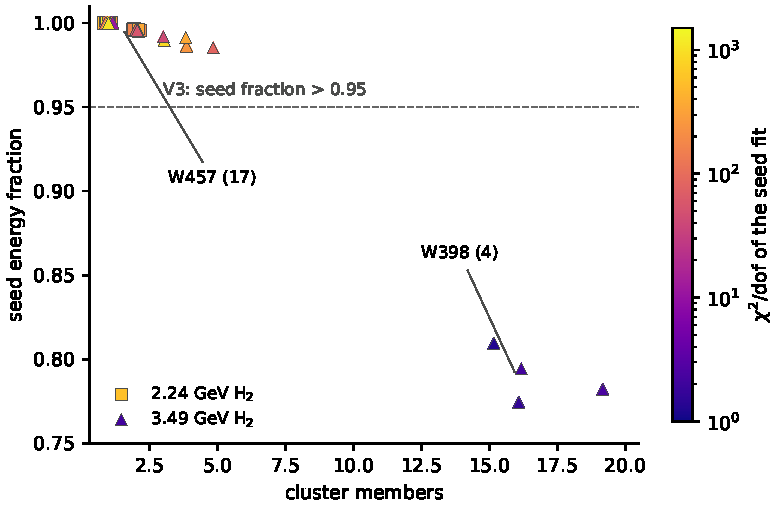
\includegraphics[width=0.75\textwidth]{exotic_saturated_seeds.pdf}
\caption{The 41 elastic-window clusters with a saturated seed (f4 or f5) in the 2.24 and 3.49\,GeV H$_2$ samples: seed energy fraction against the number of members, coloured by $\chi^2/\mathrm{dof}$ of the seed fit; the positions are jittered in $x$. Dashed: the veto V3 boundary, seed fraction 0.95. The four W398 clusters below it are real showers with a clipped high-gain seed. Source: \code{exotic\_P7\_saturated\_seeds\_20261118.tsv}.}
\label{fig:exotic_satseeds}
\end{figure}

\paragraph{Clusters under the drop policy.} The rule we proposed for this study, to use no f1 to f5 channel in the clustering or in the energy calibration, was tested in step P13 by removing every flagged channel from the hit list before clustering (arm D). The affected clusters are those of Table~\ref{tab:exotic_cluster}; what the drop changes is their fate. A dropped seed is lost in $0.048 \pm 0.002$, $0.127 \pm 0.002$, $0.103 \pm 0.003$ and $0.535 \pm 0.003\,\%$ of all clusters (0.73, 2.24, 3.49\,GeV H$_2$, Ta). The cluster then vanishes (0.020 to 0.085\,\% in hydrogen, $0.255 \pm 0.002\,\%$ in tantalum, with intervals of $\pm 0.002$\,\% or less), is re-seeded by a former member, which keeps a median 0.43 to 0.47 of the energy ($\pm 0.01$ or less), or merges into a neighbour. In the elastic window the seed loss is $0.032^{+0.013}_{-0.009}$, $0.008 \pm 0.002$, $0.009 \pm 0.002$ and $0.287 \pm 0.015\,\%$, and $0.061^{+0.016}_{-0.013}\,\%$ of the M\o ller pairs. The drop also creates clusters, as former members seed new ones and events whose fake second cluster vanishes enter the single-cluster selection: $0.018^{+0.008}_{-0.006}$, $0.051 \pm 0.004$, $0.073^{+0.009}_{-0.008}$ and $0.82 \pm 0.03\,\%$ of the calibration pool under D are new. Every fake of the V3 veto below vanishes under D (23 of 23 and 14 of 14, lower limits 96 and 93\,\%).

\subsection{Impact on yields}
\label{sec:exotic_yields}

Four vetoes and the drop policy are applied to the elastic window of the calibration chain and to the M\o ller pairs. V1 removes a cluster whose seed is flagged in any category, V2 one with any flagged member, V3 one with a saturated seed (f4 or f5) that carries more than 0.95 of the cluster energy, and V4 adds the f1 and f3 seeds to V3. D re-forms the clusters without the flagged channels and counts the window clusters of the default chain that are lost. A M\o ller pair is lost when either member is vetoed or lost, and the cost is the fraction of the population removed. V2 costs 0.10 to 0.21\,\% of the hydrogen elastic clusters ($\pm 0.02$\,\% or less), $5.98 \pm 0.07\,\%$ of the tantalum ones and $1.64^{+0.11}_{-0.10}\,\%$ of the M\o ller pairs, and is rejected; V1 and V4 differ only at 3.49\,GeV (18 against 14 clusters). Table~\ref{tab:exotic_veto} compares V3, V4 and D.

V3 removes exactly the 23 and 14 fakes of the previous subsection at 2.24 and 3.49\,GeV, keeps the four W398 showers and removes nothing at 0.73\,GeV or in tantalum. The tantalum V4 loss is concentrated in the inner ring ($0.305 \pm 0.016\,\%$ at 0 to 120\,mm). D costs 6.4 and 4.5 times V3 at 2.24 and 3.49\,GeV and removes real clusters at 0.73\,GeV, where V3 removes none. In tantalum most of the lost window clusters re-form outside the $\pm 3\sigma$ window ($1.237 \pm 0.031\,\%$), and 570 clusters enter the window in their place. The net loss is $0.875 \pm 0.037\,\%$ (Poisson error), with $0.243^{+0.044}_{-0.037}\,\%$ of the M\o ller pairs lost and $0.34 \pm 0.05\,\%$ of the pairs under D new.

V3 is adopted as the policy for the 2.24 and 3.49\,GeV hydrogen data: it costs less than 0.01\,\% and removes only fakes, so no efficiency correction follows. V4 and D are not adopted, because the calibration-impact step below shows no gain in resolution or peak position for their loss.

\begin{table}[htbp]
\centering
\caption{Cost of the vetoes V3 and V4 and of the drop policy D, in \% of the ep elastic-window clusters of the default chain (M\o ller: of the selected pairs; 68\,\% Wilson interval, count removed); $N$ is the population. A cell $<x$ removes nothing and gives the upper end of the interval. Hydrogen from the two-file sample, tantalum from the full scan; the M\o ller pairs of D are counted on the 19 split runs of step P13 (14\,785 pairs). Sources: \code{exotic\_P10\_yield\_impact\_20261118.tsv} (V3, V4) and \code{exotic\_P13\_drop\_flagged\_20261118.tsv} (D).}
\label{tab:exotic_veto}
\small
\begin{tabular}{llrlll}
\toprule
Run type & Population & $N$ & V3 & V4 & D \\
\midrule
\code{0p73GeV\_H2} & elastic & 28\,076 & $<0.004$ (0) & $0.036^{+0.013}_{-0.010}$ (10) & $0.100^{+0.021}_{-0.017}$ (28) \\
\code{2p24GeV\_H2} & elastic & 518\,921 & $0.0044^{+0.0010}_{-0.0008}$ (23) & $0.0083^{+0.0014}_{-0.0012}$ (43) & $0.0285^{+0.0024}_{-0.0022}$ (148) \\
\code{3p49GeV\_H2} & elastic & 210\,355 & $0.0067^{+0.0020}_{-0.0016}$ (14) & $0.0067^{+0.0020}_{-0.0016}$ (14) & $0.0299^{+0.0040}_{-0.0035}$ (63) \\
\code{2p24GeV\_Ta\_X17} & elastic & 130\,240 & $<0.0008$ (0) & $0.286^{+0.015}_{-0.014}$ (373) & $1.312^{+0.032}_{-0.031}$ (1709) \\
 & M\o ller & 14\,786 & $<0.007$ (0) & $0.122^{+0.032}_{-0.026}$ (18) & $0.243^{+0.044}_{-0.037}$ (36) \\
\bottomrule
\end{tabular}
\end{table}

\subsection{Energy error, calibration impact and status}
\label{sec:exotic_status}

\paragraph{Energy removed under the drop policy (P13).} Dropping every flagged channel removes from each calibration sample the energy fraction $-S$, where $S = -\sum E_{\mathrm{flagged}} / \sum E_{\mathrm{cluster}}$ is the first-order scale shift of the step P13 output (Fig.~\ref{fig:exotic_eremoved}; ratio-estimator errors). In tantalum $-S$ is $0.553 \pm 0.005\,\%$ over all clusters, $0.398 \pm 0.010\,\%$ in the elastic window and $0.089 \pm 0.014\,\%$ for the M\o ller pairs, from the f1 and f3 neighbours and seeds of the inner ring. In hydrogen $-S$ is $0.112 \pm 0.045$, $0.201 \pm 0.008$ and $0.091 \pm 0.006\,\%$ over all clusters (0.73, 2.24, 3.49\,GeV) and $0.030 \pm 0.006$, $0.0115 \pm 0.0012$ and $0.0115 \pm 0.0020\,\%$ in the elastic window, from the f3 members and, at 2.24 and 3.49\,GeV, the f4 and f5 seeds, the saturated fakes. The seed-dropped fractions are the seed losses of Section~\ref{sec:exotic_cluster}, 0.05 to 0.13\,\% of the hydrogen clusters ($\pm 0.003$\,\% or less) and $0.535 \pm 0.003\,\%$ of the tantalum ones. A correction in place (steps P8 and P9) was also tested: it shifts the tantalum elastic scale by $-0.0144 \pm 0.0003\,\%$ and no hydrogen cell by 0.01\,\%, and the gain refit absorbs it (tantalum peak $-0.0004 \pm 0.0047\,\%$).

\begin{figure}[htbp]
\centering
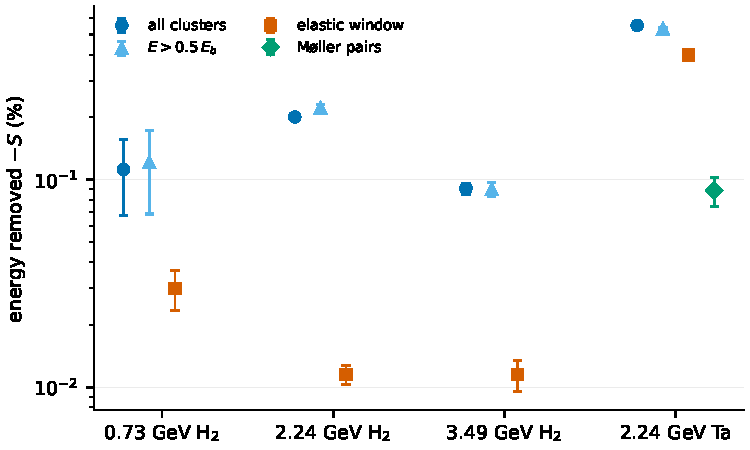
\includegraphics[width=0.5\textwidth]{exotic_energy_removed.pdf}
\caption{Energy removed from each calibration sample if every flagged channel is dropped, $-S$ with $S = -\sum E_{\mathrm{flagged}} / \sum E_{\mathrm{cluster}}$, in \%, per run type: all PbWO$_4$-seeded clusters, clusters above $0.5\,E_b$, the elastic window and the tantalum M\o ller pairs. Error bars: ratio-estimator errors. Source: \code{exotic\_P13\_drop\_flagged\_20261118.tsv}, table \code{p8\_scale}.}
\label{fig:exotic_eremoved}
\end{figure}

\paragraph{Calibration impact (P13, arms A, V3, D, D$'$).} Four arms run on identical events of the same splits (hydrogen two-file sample, 19 tantalum splits, 0.73\,GeV at $r_\perp \ge 107$\,mm) through the calibration chain of Section~\ref{sec:calib}. Arm A is the default control v3, V3 the veto of Table~\ref{tab:exotic_veto}, D the drop in both passes (clustering and gain solve, ep and the tantalum M\o ller calibration) and D$'$ the drop in the gain solve only (ep), which isolates the calibration effect. The benchmark and M\o ller scripts gained an opt-in \code{EXOTIC\_HOOK} for this, whose default path reproduces v3 exactly. With the refit on fewer splits, the arm-A values (out-of-sample $\sigma_E/E$ of 3.37, 1.78, 1.59 and 2.00\,\%, 2.12\,\% for the M\o ller pair sum; errors 0.006 to 0.06\,\%) sit above the context values of Table~\ref{tab:calibres}, and the arms are compared on the clusters present in both, with paired bootstrap errors.

No arm improves $\sigma_E/E$ or the peak anywhere. At 2.24 and 3.49\,GeV H$_2$ the D and V3 differences in $\sigma_E/E$ and peak stay within $|z| \le 1.2$. The only entries beyond $2\sigma$ are the 2.24\,GeV low tail, which D lowers by $0.017 \pm 0.006$ percentage points ($z = -2.9$, the removed fakes), and the D$'$ peak at 2.24\,GeV, $+0.0014 \pm 0.0006\,\%$ ($z = 2.3$). At 0.73\,GeV $\sigma_E/E$ and the peak do not move ($|z| \le 0.5$). Four free module-runs move beyond $2\sigma_g$ (W522 at 2.24\,GeV, W702 and W556 at 0.73\,GeV, W659 in the M\o ller calibration), the largest W702 in run 24603 by $-1.47 \pm 0.34\,\%$ ($-4.4\sigma_g$). In tantalum the ep $\sigma_E/E$ and peak stay ($+0.010 \pm 0.012$ points, $+0.005 \pm 0.010\,\%$), but the low tail grows by $0.24 \pm 0.06$ points ($z = 3.8$): the dropped f1 and f3 neighbours take $0.40 \pm 0.01\,\%$ of the elastic energy, and the gain refit only recentres the peak (D$'$ alone moves it by $+0.052 \pm 0.006\,\%$). The M\o ller pair-sum peak shifts by $+0.028 \pm 0.011\,\%$ ($z = 2.6$) at unchanged width ($-0.014 \pm 0.012$ points). The tantalum inner ring (block H) stays at the prior in the M\o ller calibration (0 of 64 module-runs free in A and D) and largely so in the ep calibration (4 free in A, 3 in D, $|\Delta g| \le 0.56\sigma_g$), so the drop does not make its gain measurable.

\paragraph{Gate decision and status.} The drop policy was the rule we proposed, and the data argue against it. It improves neither the resolution nor the peak at any run type. It costs 0.03 to 0.10\,\% of the hydrogen elastic windows, where V3 removes the same fakes for at most 0.0067\,\% (intervals in Table~\ref{tab:exotic_veto}). In tantalum it costs $0.875 \pm 0.037\,\%$ of the elastic window net and $0.243^{+0.044}_{-0.037}\,\%$ of the M\o ller pairs while it widens the low tail and shifts the M\o ller peak. The gate therefore stands: the 2.24 and 3.49\,GeV hydrogen data keep V3 (fakes only), without V4, without the drop and without in-place correction; the 0.73\,GeV hydrogen and the tantalum data get no veto, no drop and no correction. The flags remain event markers, the gated options \code{PILEUP\_BASE\_SLOPE} and \code{PILEUP\_CLIP\_SINGLE} stay off, and the full-data scan on the farm keeps all five flags, f5 included. The hydrogen numbers of this chapter rest on two files per run (the 3.49\,GeV sample is runs 24698 and 24911).
\clearpage

\section{Crosstalk study}
\label{sec:xtalk}

\paragraph{Purpose, inputs, outputs.} Crosstalk is a signal induced in one readout channel by a pulse in another channel. The study tests whether such signals degrade the fits of Section~\ref{sec:fitter} inside calorimeter clusters, and measures their rate, size and delay. Its inputs are the raw waveforms of the three H$_2$ run types of Table~\ref{tab:runs}, the template banks, the calibration constants $c_m$ and the dead-module lists. The script \code{crosstalk\_study.py} writes the $\chi^2/\mathrm{dof}$ of seed and neighbour modules per cluster-energy slice (\code{chi2\_slices.tsv}), the profile of $\chi^2/\mathrm{dof}$ against a timing difference $\delta t$, and example waveforms. The script computes no crosstalk ratio. The ratio, the delay and the link to the digitizer channels come from a separate analysis of the same scan files (\code{late\_component.tsv}), whose code is not on disk. Each result below names its source.

Two earlier versions of the study exist. The first (30 October 2026) used WaveAnalyzer pulse heights and found a coupling of about 1.0 to 1.4\,\% of the pulse in the adjacent digitizer channel. The second is kept in \code{previous\_20261107/} and \code{\_sup\_old.py}; no number, figure or statement of this note is taken from those files or from their outputs.

\subsection{Procedure}

\begin{enumerate}
\item \textbf{Scan.} Each run is read as in steps 2 to 5 of Section~\ref{sec:rates} (noise reference, event gate, bad-waveform removal, pre-cut and fit), for the PbWO$_4$ modules that are not dead. A channel is kept when its largest fitted amplitude is at least 10\,ADC and its main pulse is not truncated by the end of the readout. The noise passed to the fit is $\sigma_{\mathrm{ref}}$, and $\chi^2/\mathrm{dof}$ follows Eq.~\eqref{eq:mfchi2}.
\item \textbf{Constant-fraction time.} For the main pulse of a kept channel, $j_{\mathrm{pk}}$ is the index of the largest baseline-subtracted sample within 12\,ns (\code{CFD\_SEARCH\_NS}) of the fitted peak time $t_{0,\mathrm{main}} + t_{\mathrm{pk}}$. With $y_{1/2} = 0.5\, y_{j_{\mathrm{pk}}}$ (\code{CFD\_FRAC}) and $j_h$ the last sample before $j_{\mathrm{pk}}$ below $y_{1/2}$, the constant-fraction time and its difference to the matched-filter time are
\begin{equation}
t_{\mathrm{cf}} = 4\ns \left[ j_h + \frac{y_{1/2} - y_{j_h}}{y_{j_h + 1} - y_{j_h}} \right],
\qquad
\delta t = t_{\mathrm{cf}} - \left( t_{0,\mathrm{main}} + t_{50} \right).
\label{eq:dtcfd}
\end{equation}
Both times come from the same waveform, so $\delta t$ needs no time calibration. A pulse of the template shape has $\delta t$ near zero. A pulse of another shape, or a second pulse on the leading edge, moves $t_{\mathrm{cf}}$ and leaves $t_{0,\mathrm{main}}$ tied to the template. No $t_{\mathrm{cf}}$ is computed for a channel with a clipped sample.
\item \textbf{Clusters.} An in-window pulse has its onset between 130 and 200\,ns, and the used amplitude of a channel is its largest in-window amplitude. A channel is a local maximum when no in-window channel among its eight neighbours has a larger used amplitude. In each event the free local maximum of largest used amplitude becomes a seed, and the free in-window channels of its $3 \times 3$ neighbourhood become its members; the step repeats until no free local maximum is left. All clusters are used. The cluster energy is $E = \sum_m g_m A$ over the members, with $A$ the used amplitude and $g_m$ the gain of Section~\ref{sec:rates}.
\item \textbf{Energy slices.} Clusters are sorted into the slices of Table~\ref{tab:xtalkcuts}. For each slice the script histograms $\chi^2/\mathrm{dof}$ of the seeds and of the other members (neighbours) in 200 bins per decade, and reports the median and the 90th percentile.
\item \textbf{Timing profile.} For the seeds and the neighbours of 10 to 4000\,MeV clusters, $\chi^2/\mathrm{dof}$ is histogrammed against $\delta t$ in bins of 0.5\,ns from $-10$ to $+30\ns$; each bin with at least 20 entries gets a median and the 16 and 84\,\% quantiles.
\item \textbf{Examples.} During the scan a random sample of up to 12 seeds with $\chi^2/\mathrm{dof} > 5$ is stored per slice and run, with the raw samples and the fitted model.
\item \textbf{Late component (separate analysis).} A hit is late when $\delta t > +8\ns$. Each member of a 10 to 4000\,MeV cluster has a role: seed of a cluster with two or more members, neighbour, or isolated (single-member cluster). The adjacent digitizer channel of a hit is the channel of the same crate and slot with channel number $\pm 1$. The late fraction is tabulated by role, by hit amplitude and by the amplitude of the adjacent channel. The same tabulation against the largest geometric neighbour that is not an adjacent channel serves as the control. The coupling is the median over the late hits of the hit amplitude divided by the adjacent-channel amplitude, for adjacent amplitudes above 300\,ADC.
\end{enumerate}

\begin{table}[htbp]
\centering
\caption{Constants of the crosstalk study (\code{crosstalk\_study.py}). The fitter constants are those of Table~\ref{tab:mfconst}.}
\label{tab:xtalkcuts}
\small
\begin{tabular}{lll}
\toprule
Quantity & Value & Constant \\
\midrule
Kept channel, largest amplitude & $\ge 10\adc$ & \code{KEEP\_ADC} \\
Pre-cut on the largest sample above the baseline & $\ge 8\adc$ & \code{PRECUT\_ADC} \\
Constant fraction; search range around the peak & 0.5; $\pm 12\ns$ & \code{CFD\_FRAC}, \code{CFD\_SEARCH\_NS} \\
In-window onset & 130 to 200\,ns & \code{PRE\_LO}, \code{PRE\_HI} \\
Cluster radius in module sizes & 1.5 ($3 \times 3$ modules) & \code{CL\_RADIUS} \\
Slice edges (MeV) & 10, 50, 100, 200, 500, 1000, 2000, 3000, 4000 & \code{E\_SLICES} \\
Example seeds: $\chi^2/\mathrm{dof}$; stored per slice and run & $> 5$; 12 & \code{EX\_CHI2}, \code{EX\_KEEP} \\
Smallest number of entries of a profile bin & 20 & \code{MIN\_ENTRIES} \\
Late hit (separate analysis) & $\delta t > +8\ns$ & \\
\bottomrule
\end{tabular}
\end{table}

\subsection{Results}

\paragraph{Fit quality in clusters (current script).} The scans hold 6\,083\,537, 17\,984\,497 and 6\,792\,997 clusters at 0.73, 2.24 and 3.49\,GeV, and $t_{\mathrm{cf}}$ exists for 99.98\,\% of the seeds at 2.24\,GeV. Below the beam energy the seed $\chi^2/\mathrm{dof}$ has a median of 0.69 to 0.89 and a 90th percentile of 1.20 to 1.98 in every slice up to 2000 to 3000\,MeV (500 to 1000\,MeV at 0.73\,GeV), as Fig.~\ref{fig:xtalk_chi2} shows. Two departures stand out. At 3.49\,GeV the 90th percentile of the seeds rises from 1.30 (500 to 1000\,MeV) to 2.61 (3000 to 4000\,MeV). In the 10 to 50\,MeV slice the 90th percentile of the neighbours is 4.22 at 3.49\,GeV against 1.75 at 2.24\,GeV and 1.45 at 0.73\,GeV. The slices above the beam energy hold few clusters with very large $\chi^2/\mathrm{dof}$ (1992 seeds with median 135 at 2.24\,GeV, 3000 to 4000\,MeV) and are treated as artefacts. Figure~\ref{fig:xtalk_examples} shows six low-energy seeds with $\chi^2/\mathrm{dof} > 5$.

\begin{figure}[htbp]
\centering
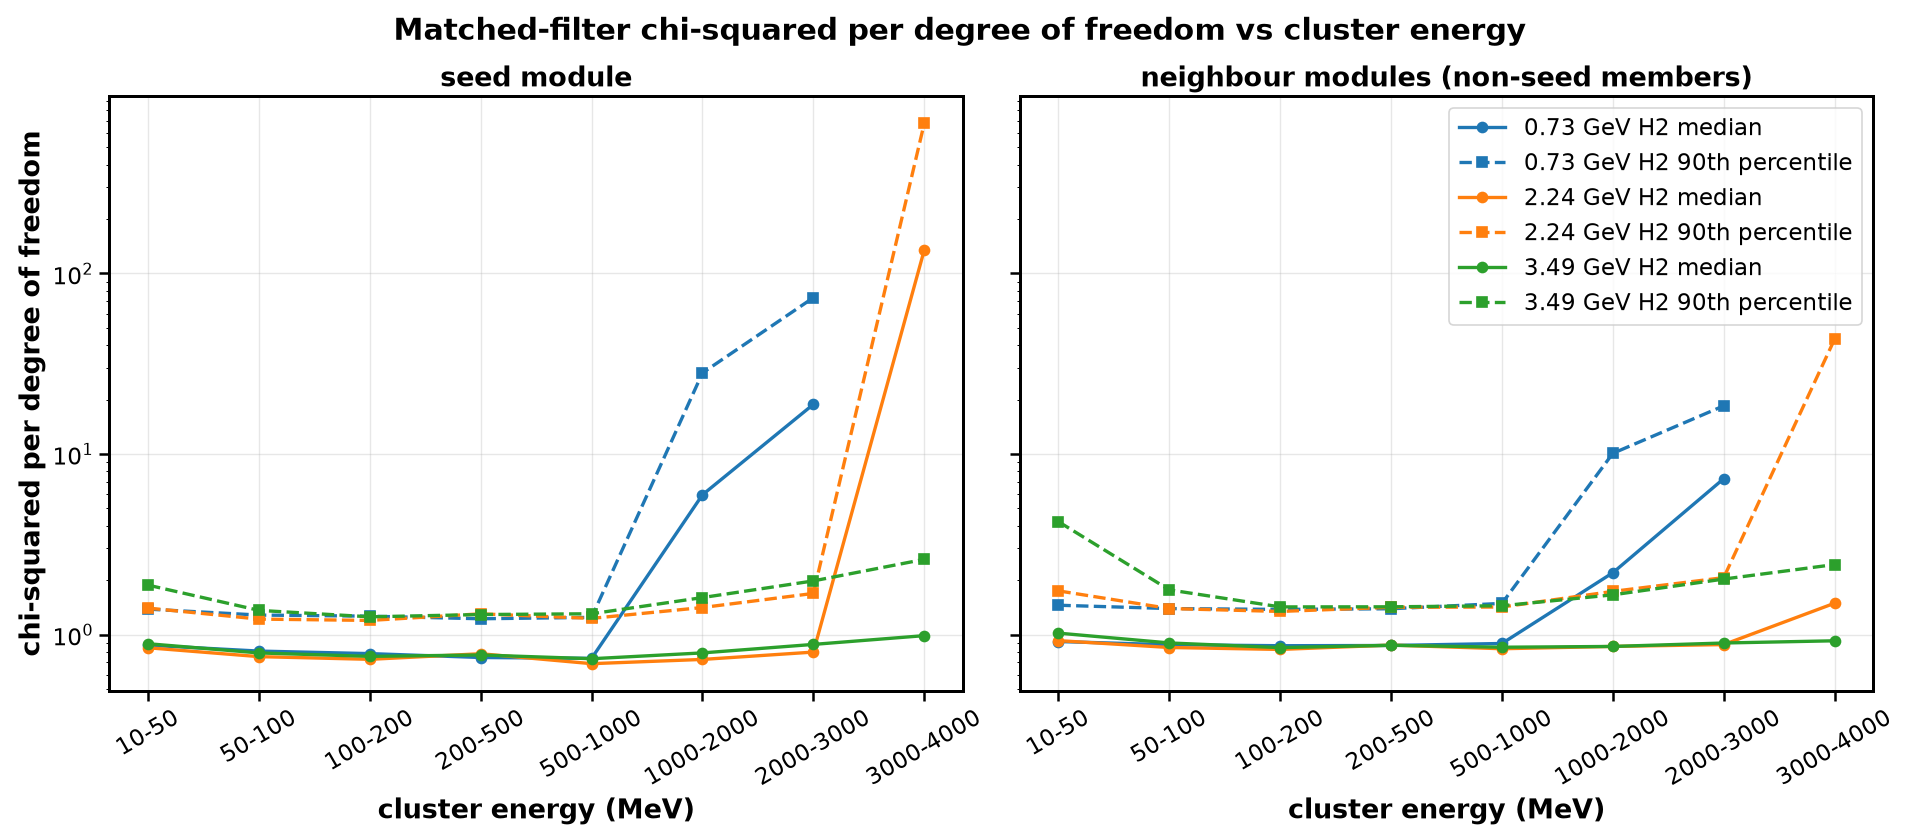
\includegraphics[width=\textwidth]{xtalk_chi2_vs_cluster_energy.png}
\caption{Median (circles, solid lines) and 90th percentile (squares, dashed lines) of the fit $\chi^2/\mathrm{dof}$ versus the cluster-energy slice, for the seed modules (left) and the neighbour modules (right). Blue: 0.73\,GeV; orange: 2.24\,GeV; green: 3.49\,GeV (H$_2$ runs). Slices with fewer than 20 entries are not drawn; the vertical axis is logarithmic. Output of the current script.}
\label{fig:xtalk_chi2}
\end{figure}

\begin{figure}[htbp]
\centering
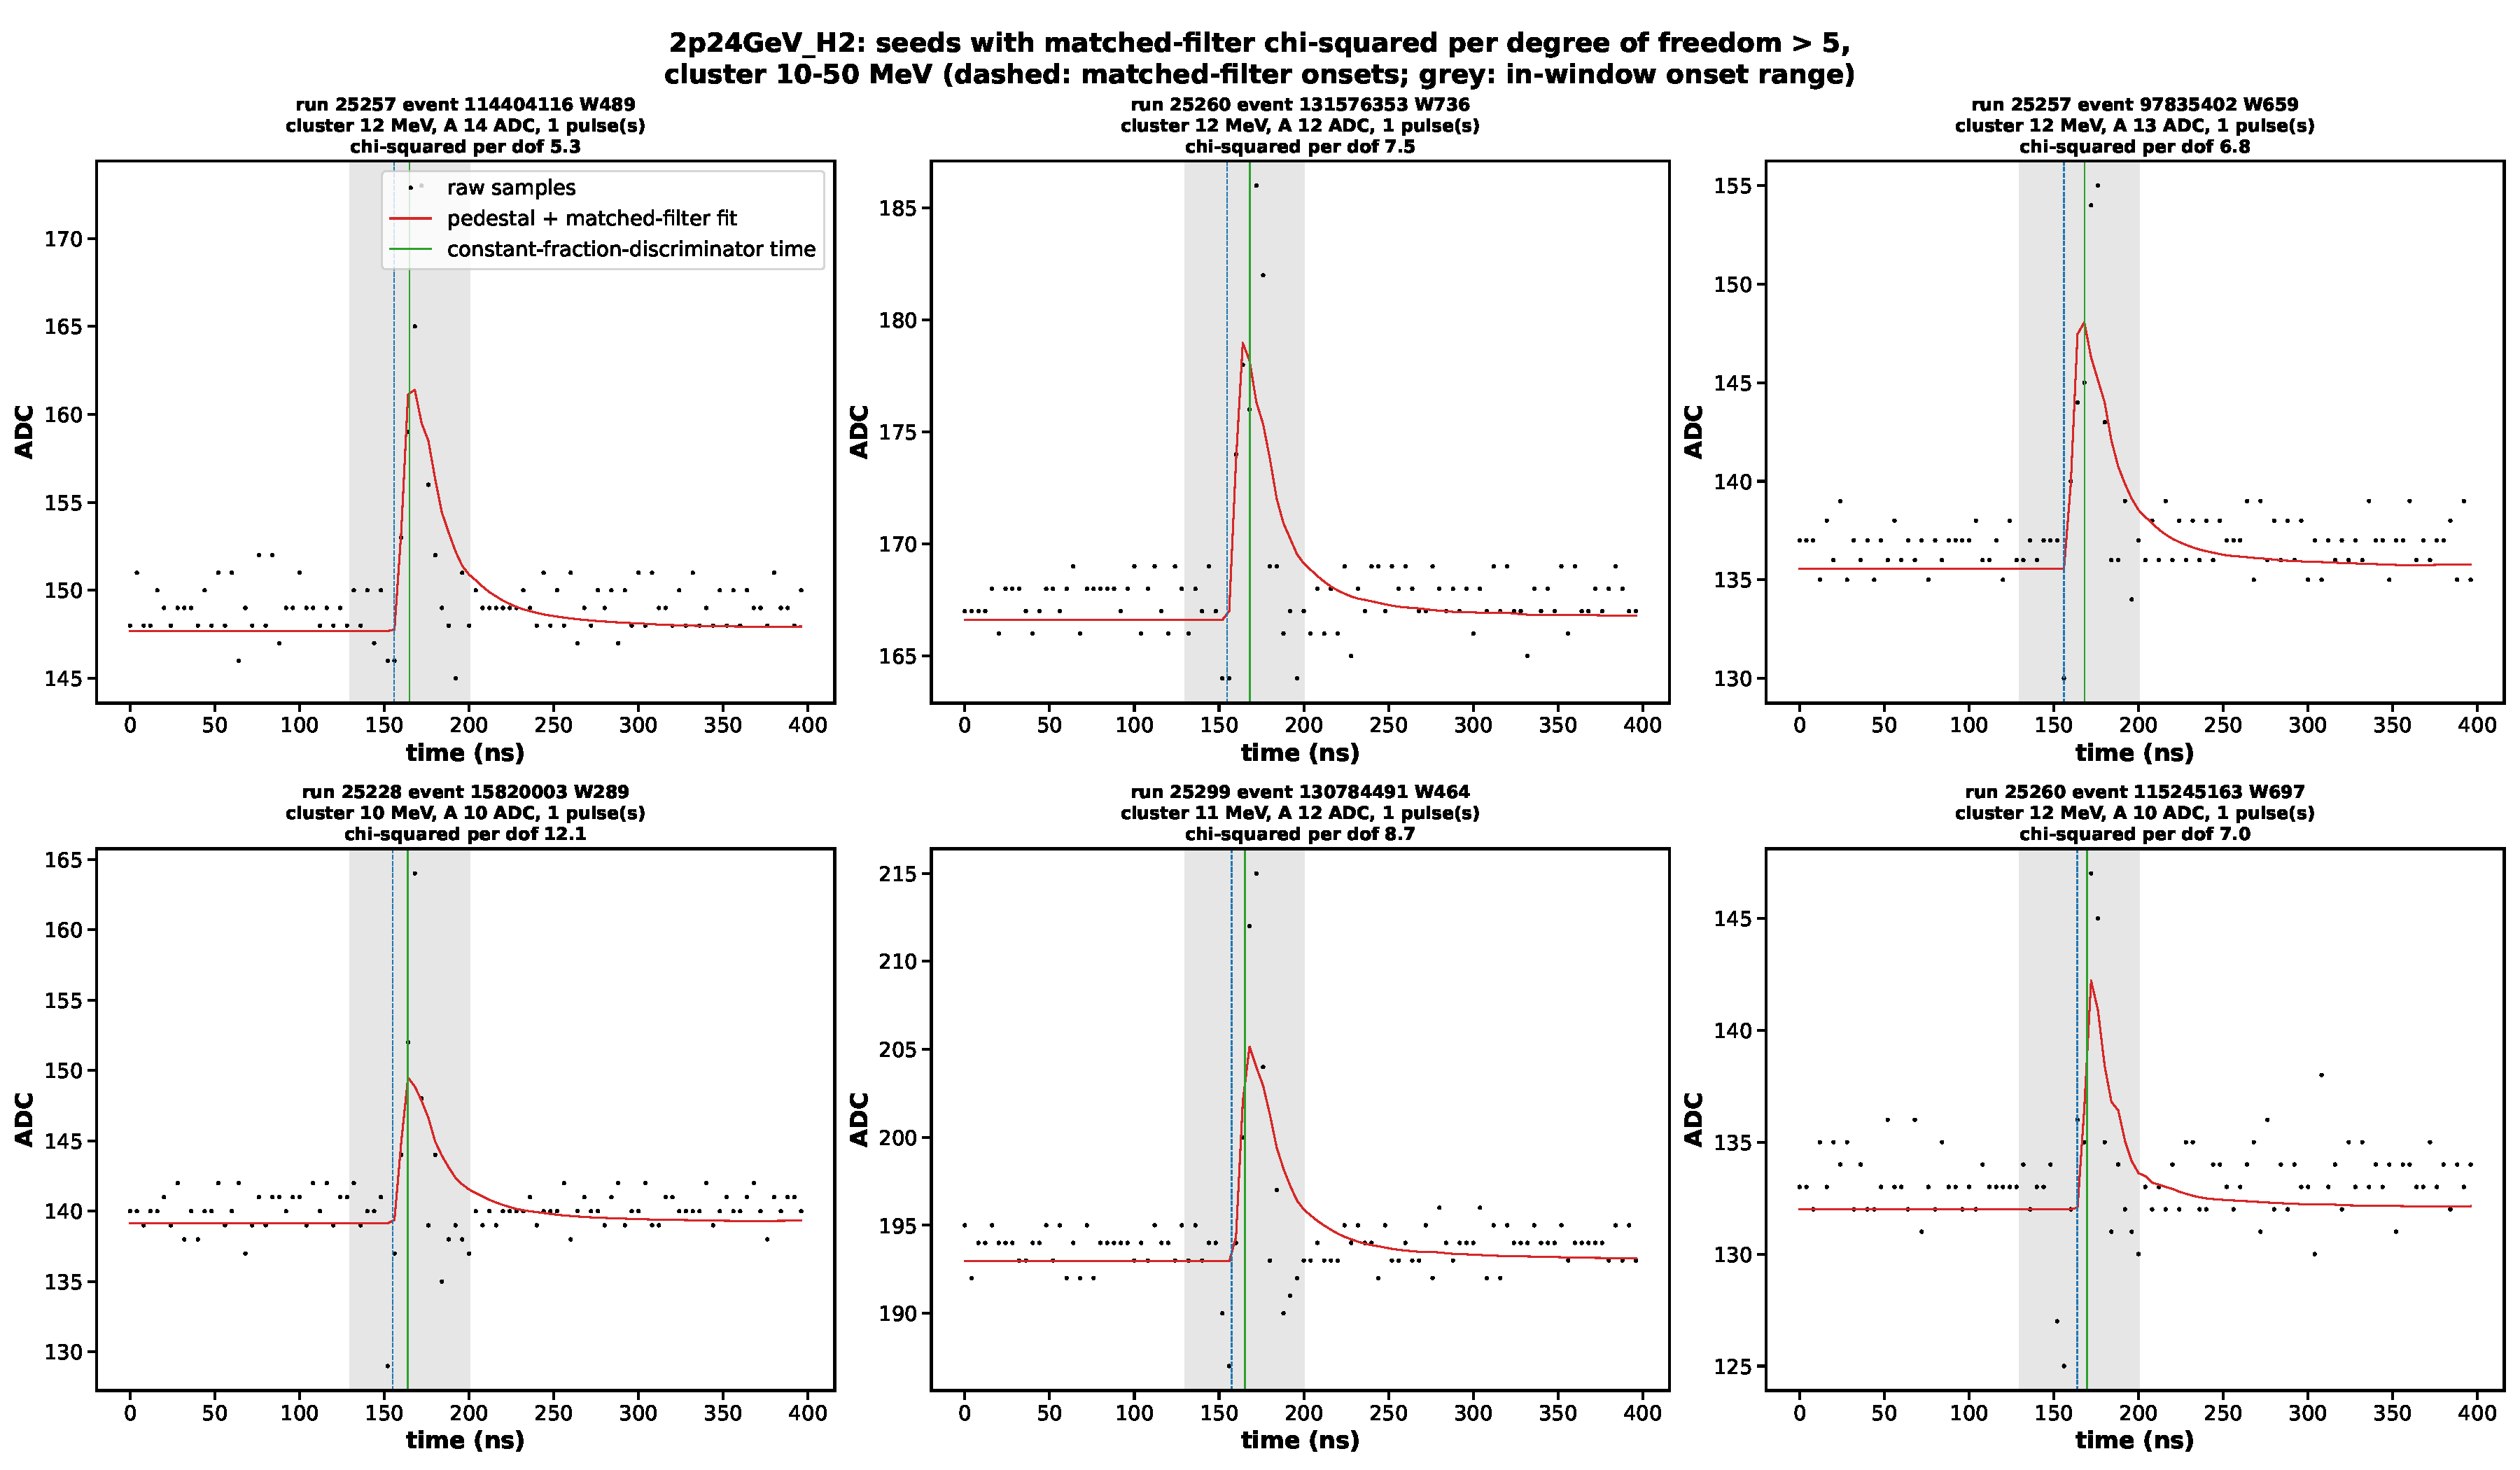
\includegraphics[width=\textwidth]{xtalk_seed_chi2_gt5_examples.pdf}
\caption{Six seeds of 10 to 50\,MeV clusters with $\chi^2/\mathrm{dof} > 5$, drawn at random from the 2.24\,GeV examples of step 6 ($\chi^2/\mathrm{dof}$ of 5.3 to 12.1, amplitudes of 10 to 14\,ADC, one fitted pulse each). Black: raw samples; red: pedestal plus fitted model; blue dashed lines: fitted onsets; green line: $t_{\mathrm{cf}}$; grey band: onset window of 130 to 200\,ns. Each title gives run, event, module, cluster energy, largest amplitude, number of pulses and $\chi^2/\mathrm{dof}$. Horizontal axis: time (ns); vertical axis: ADC.}
\label{fig:xtalk_examples}
\end{figure}

\paragraph{Late component (separate analysis, no code on disk).} The distribution of $\delta t$ has a core with median 0.0\,ns in every run type and a second population beyond $+8\ns$ (Fig.~\ref{fig:xtalk_dt}). Table~\ref{tab:xtalk} lists its size. Late hits are small: the late fraction is 0.65 and 0.93\,\% of the hits of 10 to 20\,ADC at 2.24 and 3.49\,GeV, falls by a factor of 6 to 12 for hits of 20 to 50\,ADC and is below $2 \times 10^{-7}$ above 50\,ADC. Their fits are poor, with a median $\chi^2/\mathrm{dof}$ of 5.0 and 6.2 against 0.96 and 0.97 for control hits of the same module, amplitude band and role.

\begin{table}[htbp]
\centering
\caption{Late component ($\delta t > +8\ns$) in the H$_2$ runs. Rows 1 to 10 are from \code{late\_component.tsv} (separate analysis of the current scans), row 11 from \code{seed\_chi2\_two\_peaks\_10\_50MeV.tsv}, row 12 from an unsaved diagnostic quoted in the note of 12 November 2026. Brackets give the 16 and 84\,\% quantiles; no uncertainty was computed for the medians.}
\label{tab:xtalk}
\small
\begin{tabular}{llll}
\toprule
Quantity & 0.73\,GeV & 2.24\,GeV & 3.49\,GeV \\
\midrule
Late fraction, seeds & $3.9 \times 10^{-6}$ & $4.2 \times 10^{-4}$ & $1.5 \times 10^{-3}$ \\
Late fraction, neighbours & $5.5 \times 10^{-4}$ & $2.2 \times 10^{-3}$ & $2.6 \times 10^{-3}$ \\
Late fraction, isolated hits & $1.6 \times 10^{-4}$ & $2.4 \times 10^{-3}$ & $4.9 \times 10^{-3}$ \\
Late fraction, hits of 10 to 20\,ADC & $1.2 \times 10^{-3}$ & $6.5 \times 10^{-3}$ & $9.3 \times 10^{-3}$ \\
Late fraction, hits of 20 to 50\,ADC & $2.1 \times 10^{-6}$ & $5.6 \times 10^{-4}$ & $1.6 \times 10^{-3}$ \\
Median $\chi^2/\mathrm{dof}$, late hits (control hits) & 2.19 (1.00) & 5.02 (0.96) & 6.22 (0.97) \\
Adjacent channel $> 300\adc$, late hits (control) & 44.7\,\% (12.8\,\%) & 47.3\,\% (9.5\,\%) & 41.1\,\% (9.0\,\%) \\
Late hits with adjacent channel $> 300\adc$ & 3321 & 68\,053 & 34\,211 \\
Coupling, hit over adjacent amplitude & 0.022 [0.018, 0.028] & 0.0125 [0.0095, 0.0171] & 0.0122 [0.0087, 0.0170] \\
Delay to the adjacent pulse (ns) & 12.5 [10.7, 14.4] & 13.7 [12.1, 15.4] & 13.9 [12.3, 15.5] \\
Second population, seeds of 10 to 50\,MeV clusters & 0.12\,\% & 2.7\,\% & 6.6\,\% \\
Late energy per elastic cluster, rms (MeV) & 0.66 & 2.2 & 2.8 \\
\bottomrule
\end{tabular}
\end{table}

\begin{figure}[htbp]
\centering
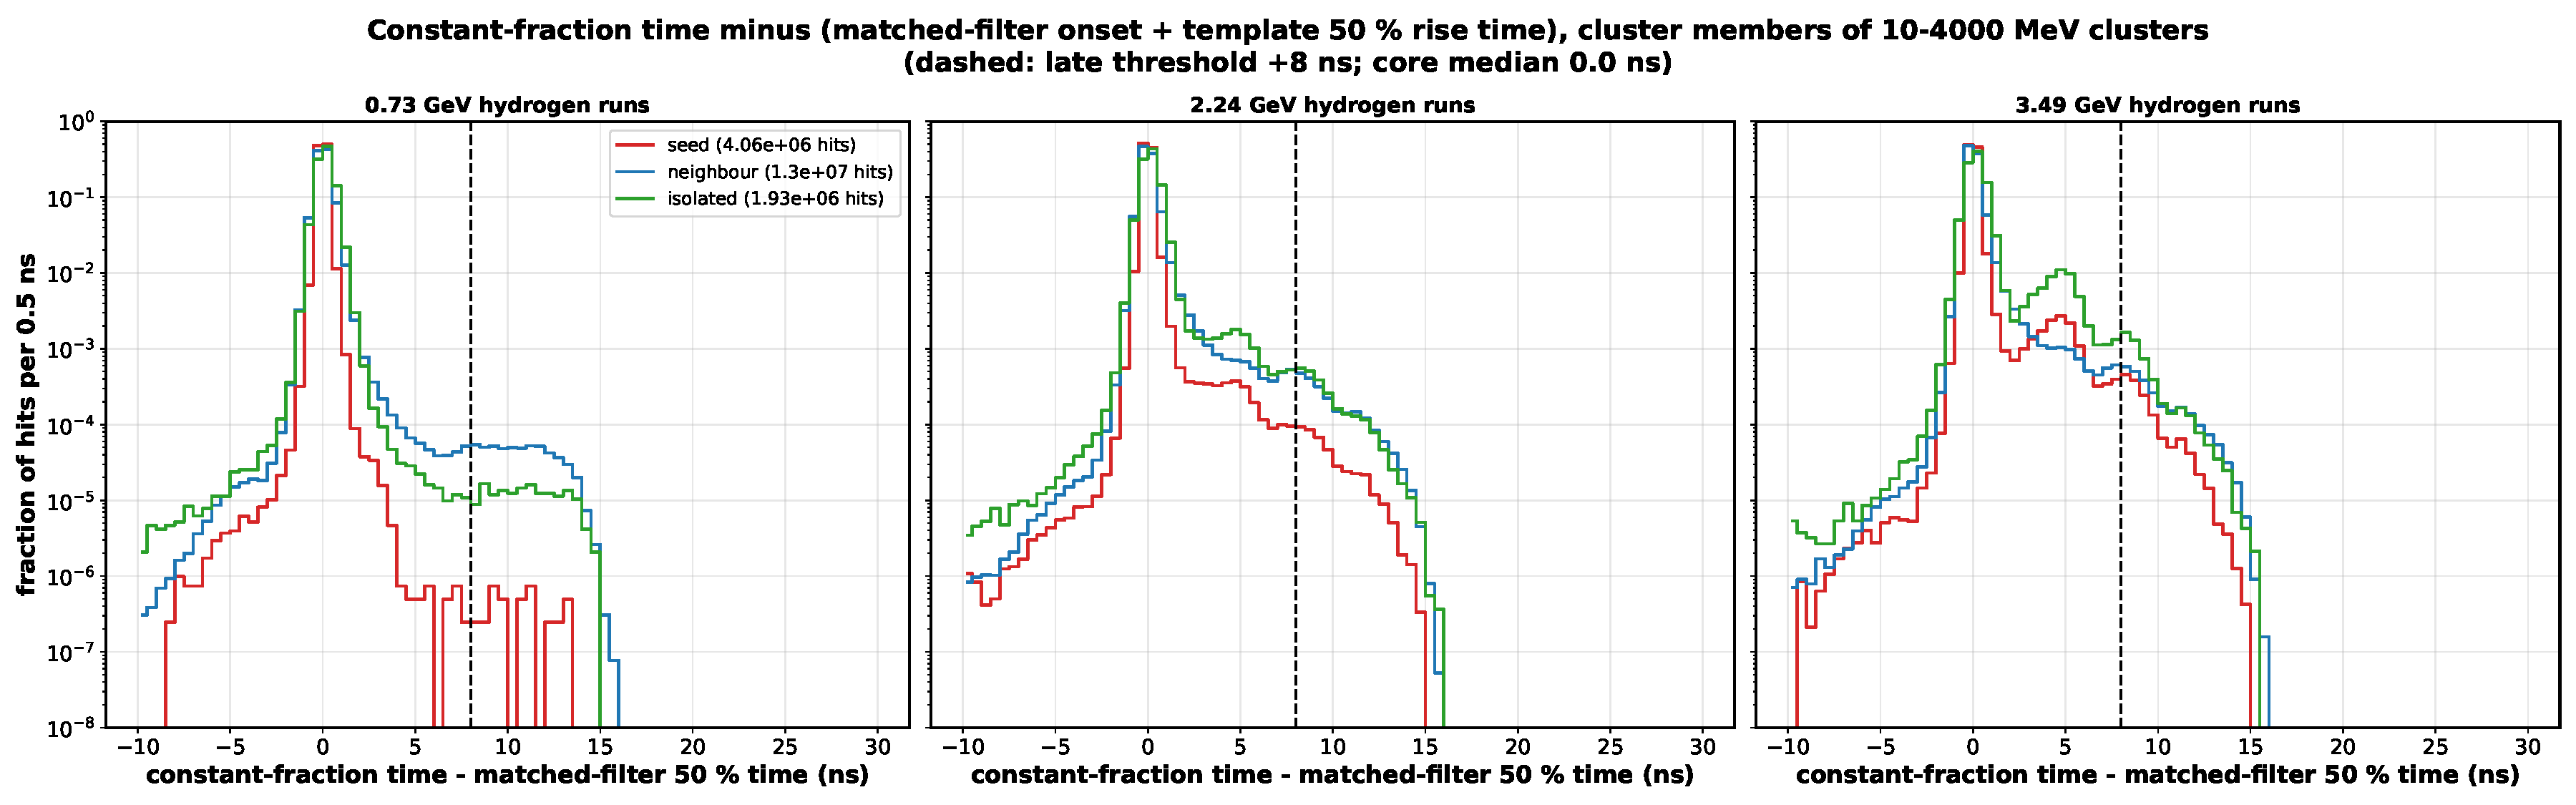
\includegraphics[width=\textwidth]{xtalk_dt_cfd_mf_by_role.pdf}
\caption{Distribution of $\delta t$ (Eq.~\eqref{eq:dtcfd}) for the members of 10 to 4000\,MeV clusters, one panel per H$_2$ beam energy. Red: seeds; blue: neighbours; green: isolated hits. Vertical axis: fraction of hits per 0.5\,ns, logarithmic. The dashed line marks $+8\ns$, the boundary of the late component. From the separate analysis.}
\label{fig:xtalk_dt}
\end{figure}

\paragraph{Origin of the late hits (separate analysis).} A late hit follows a large pulse in the adjacent digitizer channel. The adjacent channel exceeds 300\,ADC for 41 to 47\,\% of the late hits and for 9 to 13\,\% of the control hits. For hits of 10 to 20\,ADC whose adjacent channel is not a geometric neighbour, the late probability at 2.24\,GeV rises from $3.4 \times 10^{-3}$ without an adjacent pulse to 0.090, 0.107 and 0.145 for adjacent pulses of 1000 to 1500, 1500 to 2000 and above 2000\,ADC (Fig.~\ref{fig:xtalk_adj}). The same test against the largest geometric neighbour stays between $0.9 \times 10^{-3}$ and $6.7 \times 10^{-3}$. The late pulse has about 1.2\,\% of the adjacent amplitude at 2.24 and 3.49\,GeV, and its $t_{\mathrm{cf}}$ lies 13.7 to 13.9\,ns after the 50\,\% time of the adjacent pulse, against 1.5 to 1.6\,ns for control hits. These tests place the coupling between digitizer channels; it does not follow the geometry of the crystals. An adjacent channel above 300\,ADC or one of two boards (crate 2 slot 5, crate 4 slot 8) accounts for 60, 75 and 76\,\% of the late hits at the three energies; the remainder has no identified partner. Figure~\ref{fig:xtalk_map} shows where the late hits occur. An origin in the cables or the patch panel ahead of the digitizers is inferred in the status note and has not been tested.

\begin{figure}[htbp]
\centering
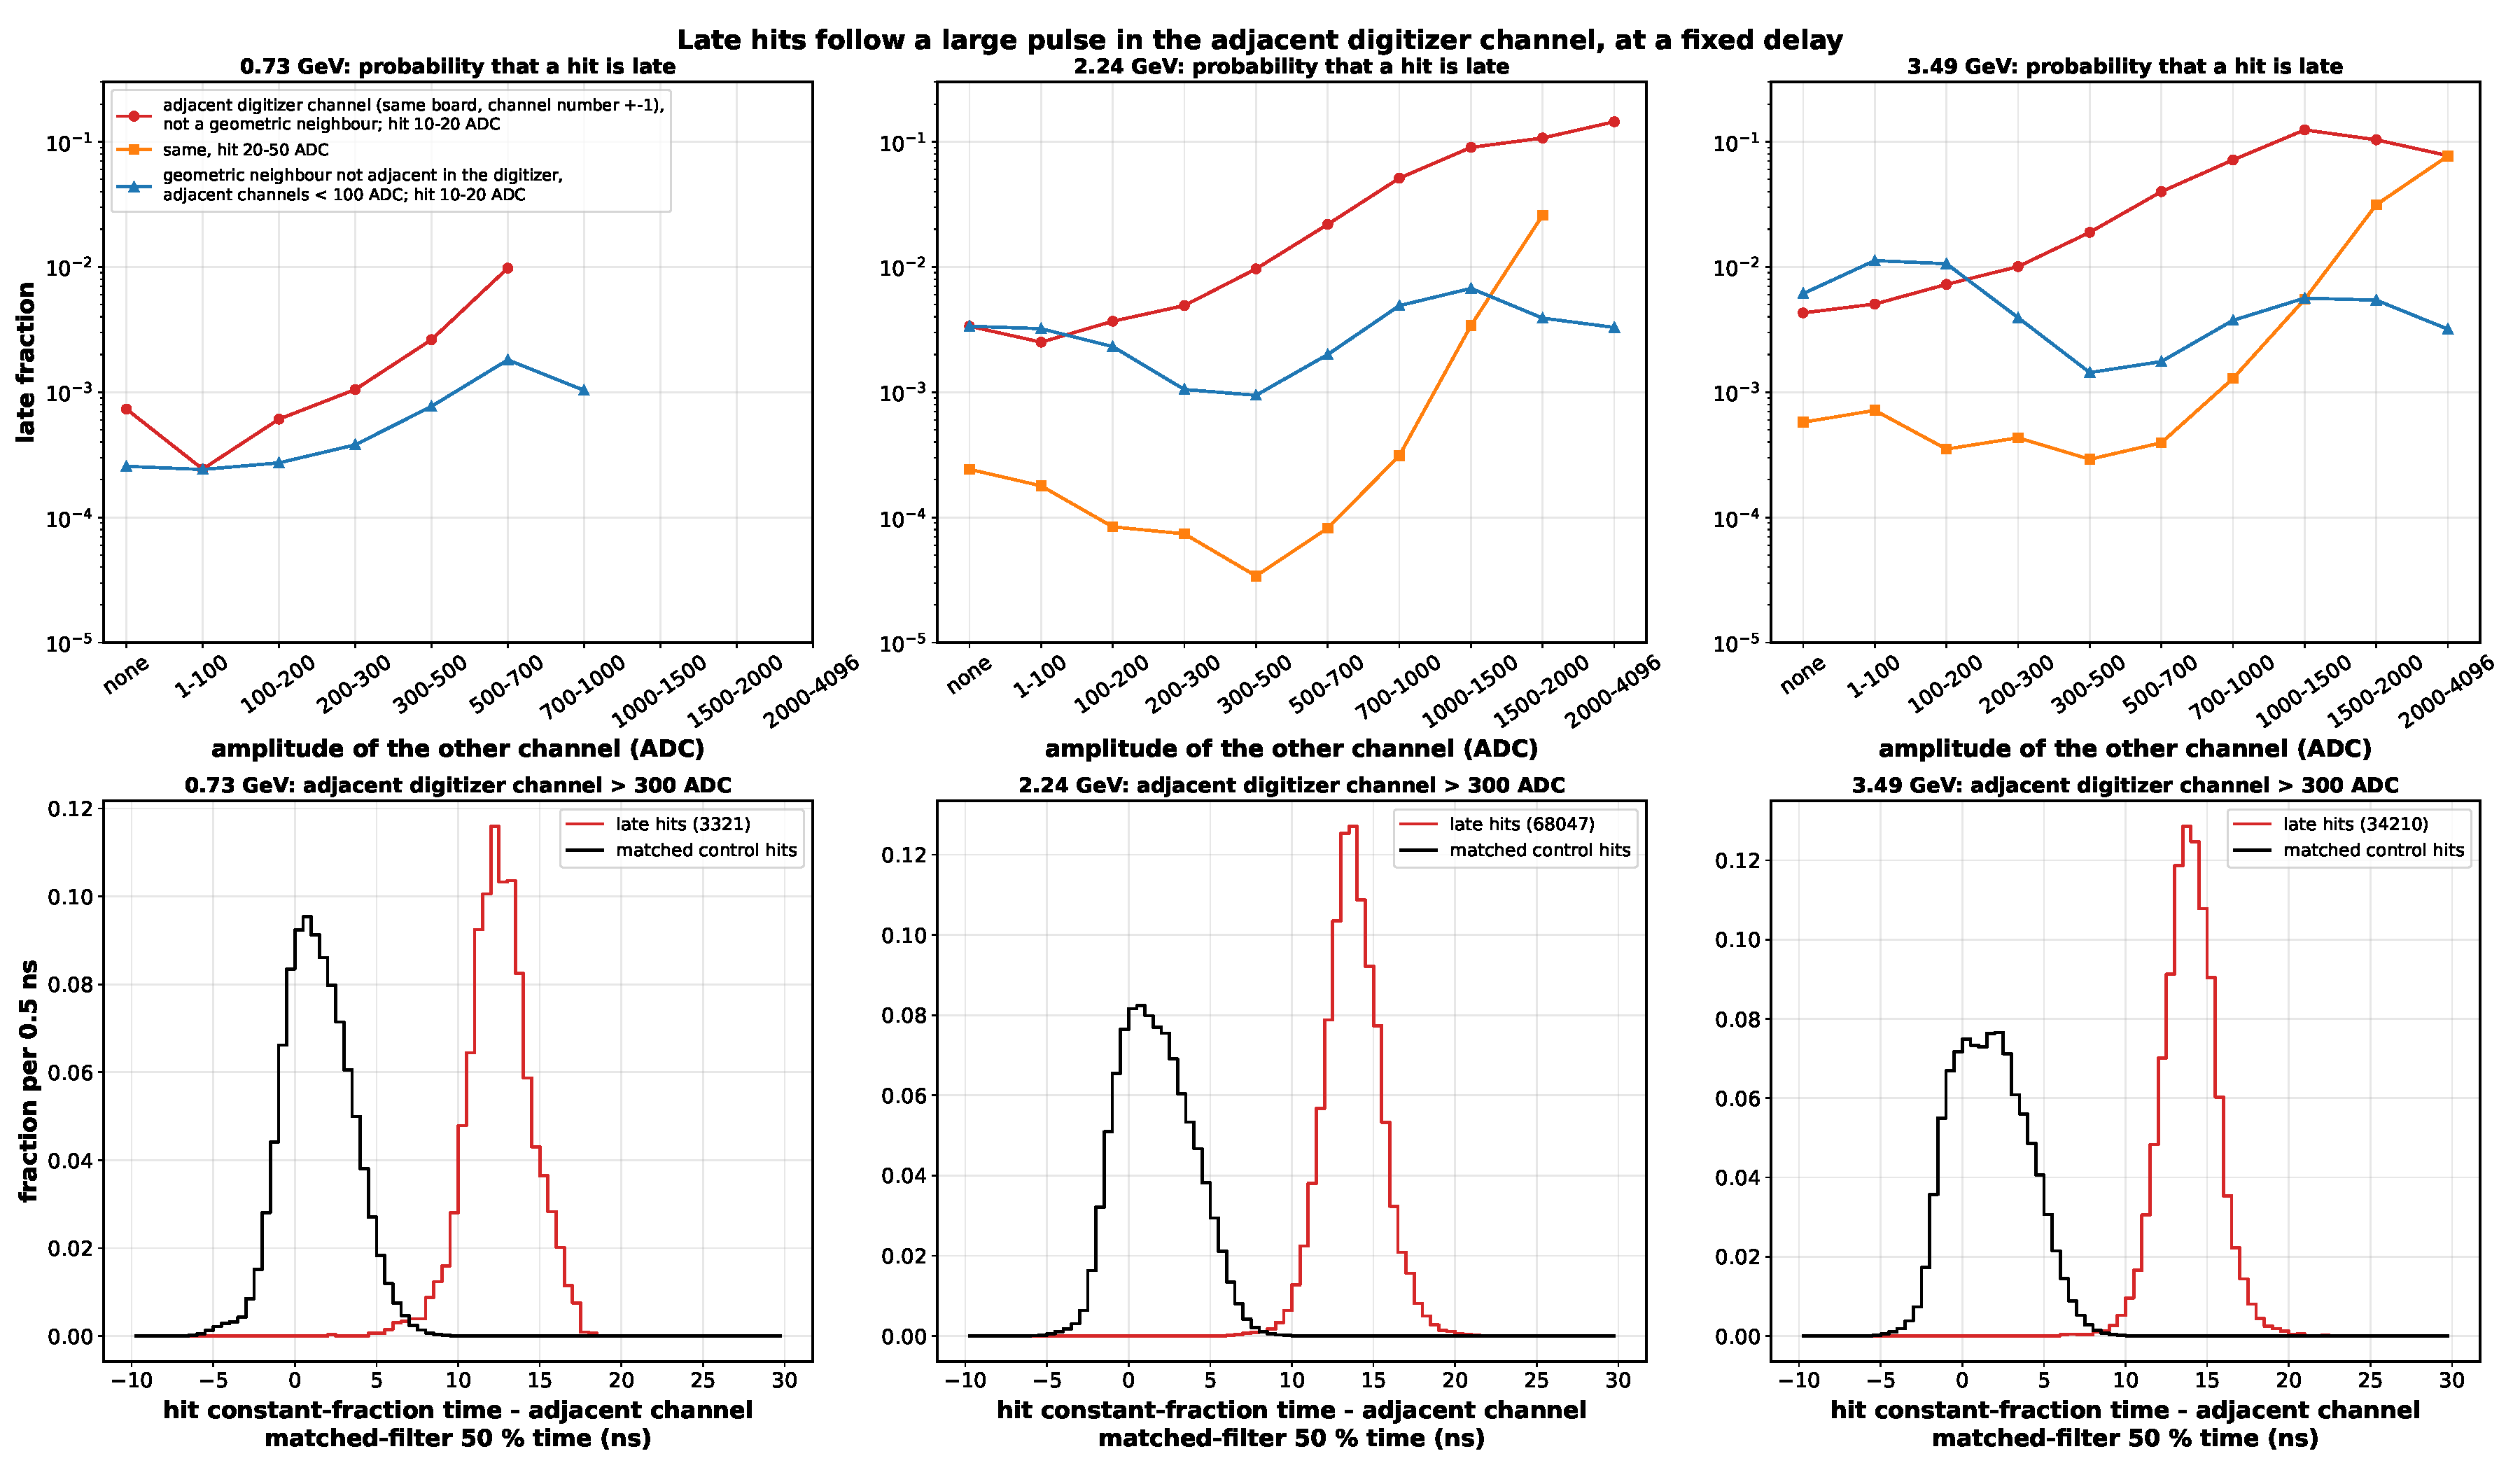
\includegraphics[width=\textwidth]{xtalk_late_vs_adjacent_amplitude.pdf}
\caption{Top: probability that a hit is late versus the amplitude of another channel (bins from no pulse to 2000--4096\,ADC). Red: the adjacent digitizer channel, when it is not a geometric neighbour, for hits of 10 to 20\,ADC; orange: the same for hits of 20 to 50\,ADC; blue: the largest geometric neighbour that is not an adjacent channel, with the adjacent channels below 100\,ADC, for hits of 10 to 20\,ADC. Bottom: $t_{\mathrm{cf}}$ of the hit minus the 50\,\% time of the adjacent pulse, for adjacent pulses above 300\,ADC; red: late hits; black: control hits. One column per H$_2$ beam energy. The hit counts in the legend (68\,047 and 34\,210) differ by 6 and 1 from Table~\ref{tab:xtalk}; the cause is not determined. From the separate analysis.}
\label{fig:xtalk_adj}
\end{figure}

\begin{figure}[htbp]
\centering
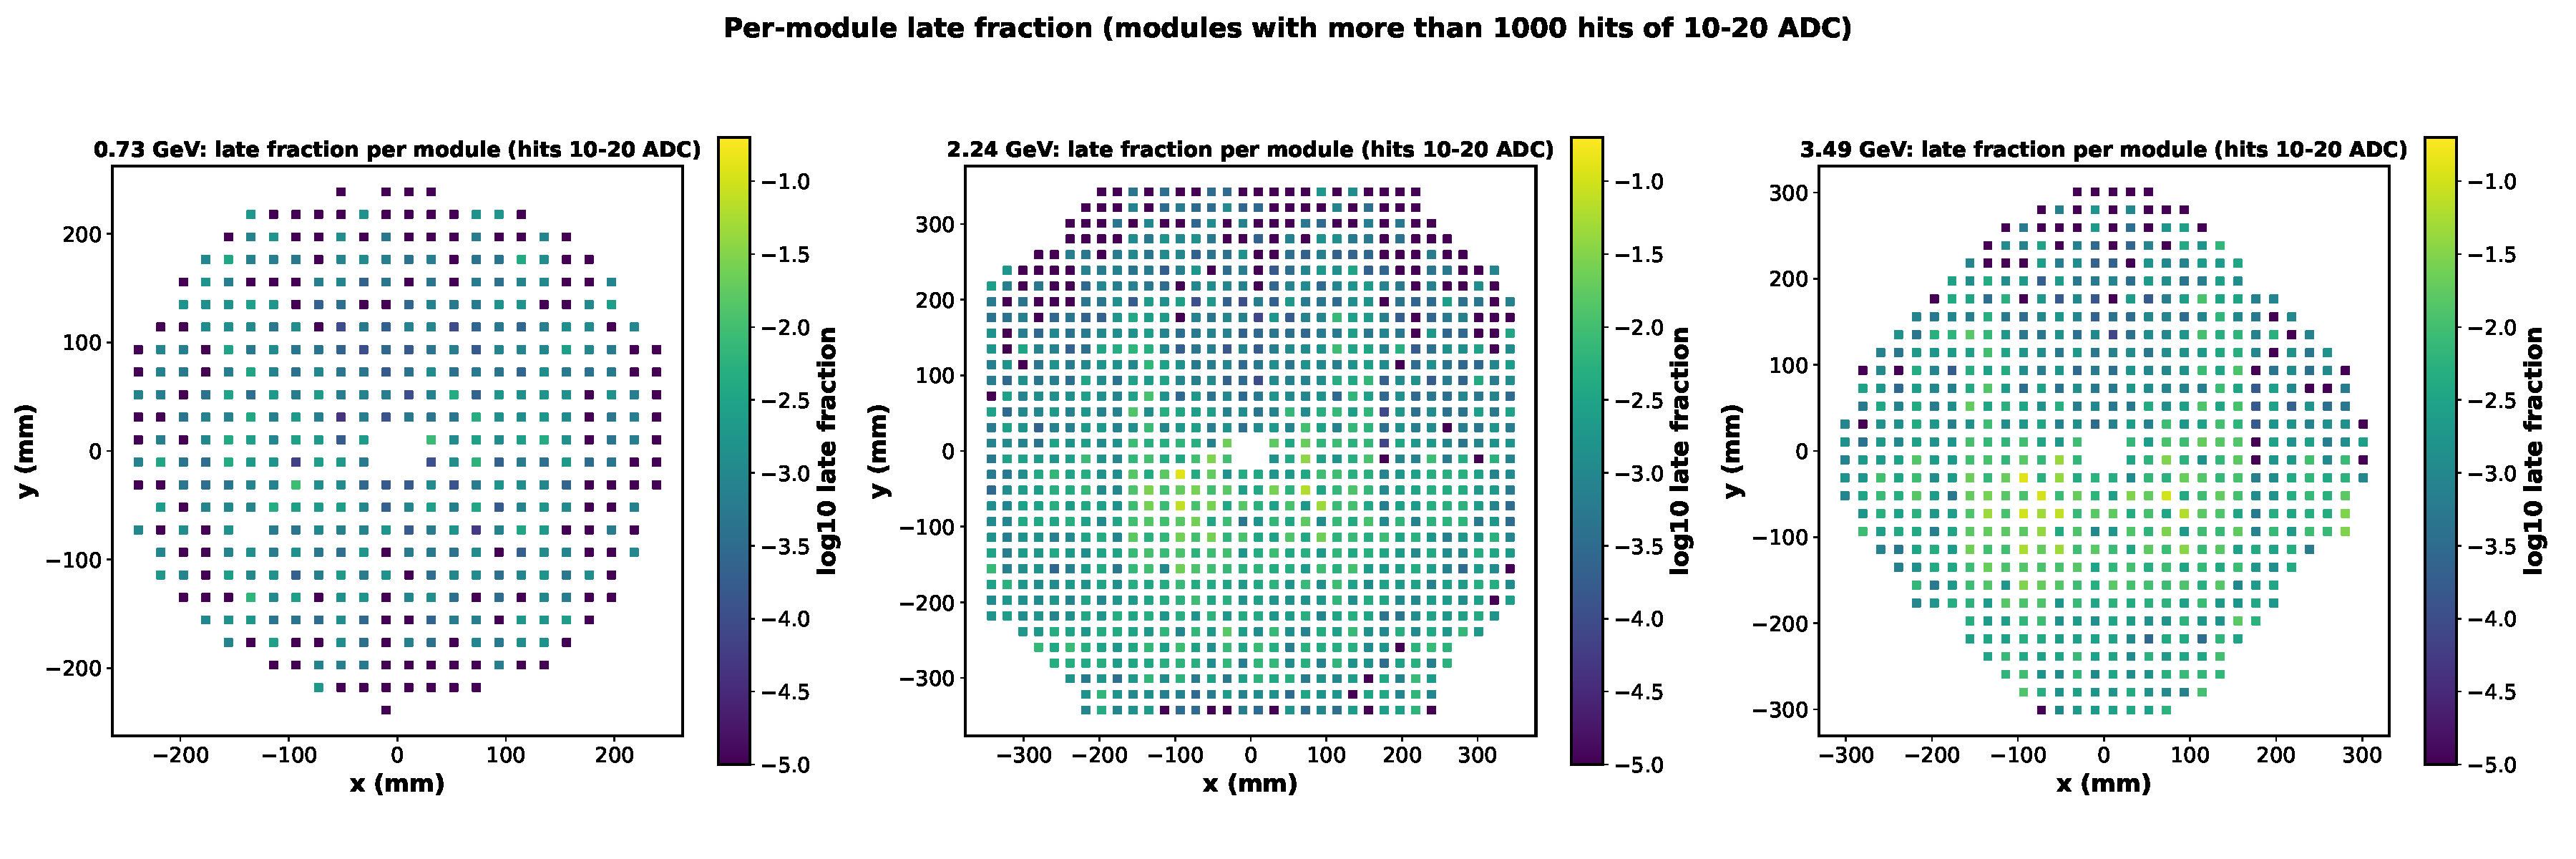
\includegraphics[width=\textwidth]{xtalk_late_fraction_map.pdf}
\caption{Late fraction per module for hits of 10 to 20\,ADC, as $\log_{10}$ on a colour scale from $-5$ to $-1$, for modules with more than 1000 such hits. Axes: module position $x$ and $y$ (mm). One panel per H$_2$ beam energy. From the separate analysis.}
\label{fig:xtalk_map}
\end{figure}

\paragraph{Low-energy seeds (separate analysis).} A fit of two Gaussians to $\log_{10}(\chi^2/\mathrm{dof})$ of the seeds of 10 to 50\,MeV clusters gives a main peak at 0.83 to 0.87 and a second population of 0.12, 2.7 and 6.6\,\% at 0.73, 2.24 and 3.49\,GeV (0.73\,GeV: constrained fit, no separated peak), peaking at 5.4 and 17 at the two higher energies. Its pulses fall in 12.2 and 6.3\,ns (median time from 90 to 10\,\% of the peak), against about 44\,ns for the main population. The short fall time matches the induced pulses of the late component.

\paragraph{Consequence for the cluster energy (unsaved diagnostic).} In elastic clusters the energy of the non-seed members with $\delta t > +8\ns$ has an rms of 0.66, 2.2 and 2.8\,MeV at 0.73, 2.24 and 3.49\,GeV, which is 0.10 and 0.08\,\% of the beam energy at the two higher energies. The number is quoted from the note of 12 November 2026; its code and output were not saved. Its effect on the resolution of Section~\ref{sec:calib} is below 0.03 percentage points. A veto of late hits would act on the false clusters of 10 to 100\,MeV: 0.26 and 0.51\,\% of the isolated 10 to 50\,MeV clusters at 2.24 and 3.49\,GeV are late.

\paragraph{Limits of the study.} The medians and percentiles carry no uncertainties. The coupling is a median of per-hit ratios in a selected amplitude band; the control hits give 2.0 to 2.6\,\%, so the ratio by itself does not identify an induced pulse. The tantalum runs are not scanned. The clustering applies no time requirement between a member and its seed beyond the common onset window, so late hits inside the window count as members. The main pulse of $\delta t$ is the largest pulse of the channel, while the clustering uses the largest in-window pulse; the two differ in some multi-pulse channels. The late-component and two-population analyses cannot be rerun from the repository.
\clearpage

\section{Summary of the waveform analysis}
\label{sec:summary}

Table~\ref{tab:summary} collects the key numbers of Sections~\ref{sec:selection} to \ref{sec:xtalk}; each row points to the section that defines the quantity and names its data set.

\begin{table}[htbp]
\centering
\caption{Key numbers of the waveform analysis. Triples are in the order 0.73, 2.24, 3.49\,GeV (H$_2$ runs) or $A_1 = 300$, 1000, 3000\,ADC (generated events).}
\label{tab:summary}
\small
\begin{tabular}{p{0.15\textwidth}p{0.42\textwidth}p{0.23\textwidth}l}
\toprule
Part & Quantity & Value & Section \\
\midrule
Templates & modules with their own template (\code{2p24GeV\_H2}) & 1146 of 1152 & \ref{sec:build} \\
 & of these, general pool; single pulse & 136; 5 & \ref{sec:build} \\
 & median pool size; median alignment rms & 86 pulses; 0.10 to 0.12\,ns & \ref{sec:build} \\
\midrule
Fitter & largest number of pulses; candidate separation & 6; 8\,ns & \ref{sec:fitter} \\
\midrule
Rates & channel cut rate, H$_2$ (\%) & 0.955, 0.545, 0.280 & \ref{sec:rates} \\
 & channel cut rate, tantalum (\%) & 7.331 & \ref{sec:rates} \\
 & channels with two or more pulses, H$_2$ (\%) & 1.849, 2.862, 3.207 & \ref{sec:rates} \\
 & channels with two or more pulses, tantalum (\%) & 22.6 & \ref{sec:rates} \\
 & cluster cut rate, all extras, H$_2$ (\%) & 1.460, 0.825, 0.423 & \ref{sec:rates} \\
 & cut rate of the eight hottest modules, tantalum (\%) & 26.0 to 32.3 & \ref{sec:rates}, \ref{app:hot} \\
\midrule
Generator & events; two-pulse cells of 10\,000 events & 19\,510\,000; 1936 & \ref{sec:generator} \\
\midrule
Deconvolution & efficiency, $\rho = 0.1$, $\Delta t = +8\ns$ (\%) & 49.1, 83.4, 97.0 & \ref{sec:deconv} \\
 & efficiency, $\rho = 0.1$, $\Delta t = +12\ns$ (\%) & 92.9, 99.8, 99.9 & \ref{sec:deconv} \\
 & efficiency, $\rho = 0.05$, $\Delta t = +12\ns$ (\%) & 29.2, 65.0, 85.9 & \ref{sec:deconv} \\
 & false-positive rate of the controls (\%) & 0.054, 0, 0 & \ref{sec:deconv} \\
 & width of the main-pulse pull, controls (\%) & 0.99--1.08, 0.52--0.55, 0.29--0.31 & \ref{sec:deconv} \\
\midrule
Crosstalk & late fraction, hits of 10 to 20\,ADC (\%) & 0.12, 0.65, 0.93 & \ref{sec:xtalk} \\
 & late pulse over adjacent-channel pulse (\%) & 2.2, 1.25, 1.22 & \ref{sec:xtalk} \\
 & delay to the adjacent pulse (ns) & 12.5, 13.7, 13.9 & \ref{sec:xtalk} \\
 & late energy per elastic cluster, rms (MeV), unsaved diagnostic & 0.66, 2.2, 2.8 & \ref{sec:xtalk} \\
\bottomrule
\end{tabular}
\end{table}

\paragraph{Open points.}
\begin{enumerate}
\item The fitted baseline offset $\delta p$ sits at its limit of one $\sigma$ in 13 to 24\,\% of the kept channels (Table~\ref{tab:rates}). A flag in place of the limit has not been tried.
\item The hydrogen cut rates are upper limits (Section~\ref{sec:rates}). The cut of Eq.~\eqref{eq:cutpulse} starts at $\rho = 0.1$ and 8\,ns, where the efficiency of Section~\ref{sec:deconv} is between 49 and 97\,\%, and a secondary pulse with $\rho = 0.05$ is first resolved at 12\,ns. A correction of the measured rates for this efficiency has not been made.
\item The candidate separation was lowered from 12 to 8\,ns on the generated events. The check on data (run 25320) is pending.
\item W335 rings in the 0.73\,GeV runs and is a candidate for the dead-module list.
\item The generator applies one shape perturbation to both pulses of an event and generates white noise (Section~\ref{sec:generator}). The study cannot be rerun until the generated file and the bank agree again (Section~\ref{sec:deconv}).
\item Two failures of the fitter are not explained: $\rho = 2$ at $\Delta t = -128\ns$, and the lower efficiency of W494.
\item Templates built from a single pulse are noisy (5 modules in the \code{2p24GeV\_H2} build).
\item At 3.49\,GeV 1.97\,\% of the events have a kept channel and no in-window pulse (Section~\ref{sec:rates}).
\item A raised baseline (W121) and a pulse wider than the template (W493) give extras that pass the second-pulse cut (Section~\ref{sec:rates}). Section~\ref{sec:exotic} flags the W121 waveform as wide (f2); the W493 event has not been evaluated.
\item The late-component analysis of Section~\ref{sec:xtalk} has no code in the repository, and a veto of induced pulses is not implemented. Between 24 and 40\,\% of the late hits have no identified partner channel.
\end{enumerate}
\clearpage
\section{Energy calibration}\label{sec:calib}

\emph{Status: this section describes the calibration chain adopted on 14 November 2026 (``control v3'' of the improvement programme) and its results. Every number is a present value for the stated data set; the open items of Section~\ref{sec:calibopen} remain.}

The calibration converts the fitted pulse amplitudes of Section~\ref{sec:fitter} into cluster energies and is judged by the width of the elastic peak and by the separation of the elastic peak from the pion threshold. It is implemented in \code{energy\_resolution\_benchmark.py} (working tree of 14 November 2026); the description below follows that script, the result notes \code{energy\_resolution/improvement/P*.md} and \code{control\_phase2*.md}, and the decision record of the plan of 12 November 2026. The inputs are the run-type template banks of Section~\ref{sec:templates}, the calibration files named by the run information, the module time offsets of \code{hycal\_time\_offsets/time\_calib.json}, the correction tables under \code{energy\_resolution/tables/} and the runs of Table~\ref{tab:runs}, with run 24937 excluded (24\,k events, gain solve not converged) and the three earlier 3.49\,GeV runs 24386, 24503 and 24512 as a replication set.

The chain grew in three steps from the reference path of 12 November (``legacy''): v1 added the calibrated time gate and the log-weighted position, v2 the cluster-shape factor and the 4\,ns tantalum gate, v3 the below-threshold correction, the residual phase correction and the ring-scoped gain constants. Section~\ref{sec:calibchain} lists the v3 chain in processing order, Section~\ref{sec:calibcomp} compares the four states and names what was tested and rejected, Section~\ref{sec:calibres} gives the v3 results and Section~\ref{sec:calibopen} what is open.

\subsection{Calibration chain, v3}\label{sec:calibchain}

The steps are in the order in which the code applies them to one split (one EVIO file). Steps 1 to 5 act on hits, steps 6 to 8 select events and define the elastic sample, steps 9 to 13 are the fitted corrections and steps 14 and 15 the measurement. The gains, ring gains, position correction and shape factor of steps 10, 11 and 13 are fitted on the elastic sample of the legacy path and then applied to every gated path; the table of step~9 is fitted on the peak clusters of the control gate.

\begin{enumerate}
\item \textbf{Calibration basis.} For each run the run-information file gives the beam energy, the calibration file and the dead modules. The linear factor $c_m$ of that file converts the pulse integral of module $m$ to MeV. The 576 lead-glass modules have factor zero in every calibration file.
\item \textbf{Energy and time of a hit.} The hit energy is the template-fit amplitude scaled to an integral,
\begin{equation}
E_{\mathrm{hit}} = c_m\, I_m\, \iota_m(\varphi)\, A ,
\label{eq:ehit}
\end{equation}
with $A$ the fitted amplitude of the pulse (Section~\ref{sec:fitter}), $I_m$ the integral of the unit-peak template of the module and $\iota_m(\varphi)$ the sampled template integral at the sub-sample onset phase $\varphi = -(t_0 \bmod 4\ns)/4\ns$ divided by its mean over phase, tabulated at 256 phases (\code{PHASE\_CORR}). The hit time is $t = t_0 + t_{50}$, the onset plus the half-maximum time of the template, and a pulse is stored when $100 < t < 200\ns$. Clipped channels without a usable pulse and lead-glass channels use the WaveAnalyzer integral times $c_m$.
\item \textbf{Module time offsets.} Before clustering, the offset of module $m$ from \code{time\_calib.json} is subtracted from every hit time (\code{TIME\_OFFSETS}); unresolved modules and the lead glass keep offset zero. The robust width of the seed--member time difference falls from 2.3, 2.8, 3.1 and 3.2\,ns to 0.7, 1.1, 1.5 and 1.4\,ns at 0.73, 2.24 and 3.49\,GeV and for tantalum (\code{P15\_tgate\_calibrated.md}). The offsets are applied at report time; the scans are not redone.
\item \textbf{Residual phase correction.} The table $\iota_m(\varphi)$ leaves a first harmonic of the response in $\varphi$ of amplitude $4.5 \times 10^{-3}$ at 2.24\,GeV (\code{P10\_phase\_corr.md}): the table correction has about 0.75 of the needed size and is rotated by about 25 degrees. Every PbWO$_4$ hit with a fitted pulse is therefore divided by
\begin{equation}
1 + c_1 \cos\vartheta + s_1 \sin\vartheta + c_2 \cos 2\vartheta + s_2 \sin 2\vartheta, \qquad \vartheta = 2\pi\varphi ,
\label{eq:phaseresid}
\end{equation}
with $c_2$, $s_2$ common to all modules and $c_1$, $s_1$ per module where a module row exists (form M1: global harmonics $k = 1, 2$ plus a per-module $k = 1$ table, ridge parameter 100). One table per run type is stored in \code{tables/phase\_resid/M1\_<RT>.tsv}, fitted on the even and the odd splits of each run separately; a split is always corrected with the table of the other half.
\item \textbf{Time-gated island clustering.} Hits are sorted by energy. The seed of a cluster is the largest unconsumed hit of at least 30\,MeV (\code{MIN\_CENTER\_E}). The island grows over neighbouring modules, and a neighbour contributes its largest unconsumed hit with $|t - t_{\mathrm{seed}}| \le G$; the window is symmetric. The gate $G$ is fixed per run type (\code{CONTROL\_GATE}): 20\,ns at 0.73\,GeV, 16\,ns at 2.24 and 3.49\,GeV and 4\,ns for tantalum. The reference path (``legacy'') has no gate and passes only the largest in-window pulse of each module. The H$_2$ gates are the minima of the out-of-sample scan with calibrated times; the tantalum gate is set by the tails (Section~\ref{sec:calibcomp}).
\item \textbf{Event selection.} With $k_E = E_b / 2239.51\mev$, an event is used when it has exactly one cluster above $500\mev \times k_E$. The seed module must hold at least $200\mev \times k_E$, lie within $r_\perp < 200$\,mm of the beam axis (module centre) and lie outside the block of rows 15 to 20 and columns 15 to 20 around the central hole. These seeds form the \emph{pool}; the headline numbers are pool numbers.
\item \textbf{Detector regions.} By the radius of the seed-module centre the PbWO$_4$ part is divided into I1 ($r_\perp < 120$\,mm), I2 (120 to 160\,mm), I3 (160 to 200\,mm), M (200 to 300\,mm) and O ($r_\perp \ge 300$\,mm); H is the hole block of step~6 and T the outermost two PbWO$_4$ layers, and these two take precedence over the radius. The pool is I1 $+$ I2 $+$ I3. Region rows are evaluated with the pool's corrections unless step~11 trains a ring.
\item \textbf{Elastic reference energy.} The seed-module centre lies at polar angle $\theta = \arctan(r_\perp/z_{\mathrm{HyCal}})$, with $z_{\mathrm{HyCal}}$ the distance from the target to the calorimeter. The expected energy of the cluster is
\begin{equation}
E'(\theta) = \frac{E_b\, M}{M + E_b (1 - \cos\theta)} - \frac{2.056\mev}{\cos\theta},
\label{eq:eprime}
\end{equation}
with $M$ the target mass (proton, or tantalum at 180.948\,u) and the second term the energy loss in the material before the calorimeter (four terms in the code, summing to 2.056\,MeV at normal incidence).
\item \textbf{Below-threshold correction.} The readout threshold is the firmware value of 10\,ADC, which is 9.5 to 9.7\,MeV in the median and 5.3 to 13.3\,MeV across modules (\code{P12\_threshold.md}). Energy of cluster members below it is lost, and the loss fluctuates from event to event. Following the KTeV treatment, every usable PbWO$_4$ module of the $5 \times 5$ window around the seed that has no stored hit in the event receives a virtual member of energy $c(d, T_m)\, T_m$. Here $T_m$ is the threshold of the module in MeV and $d$ the distance of the module centre from the cluster position in module sizes (bins of 0.125 up to 3); $T_m$ falls into one of three classes with edges at 9.0 and 9.8\,MeV. The 72 coefficients are fitted on the peak clusters of the control chain from the distribution of the energy over threshold, with the part below $1.2\,T_m$ modelled as a truncated exponential; $c$ is 0.6 to 0.7 where few window modules are absent and 0.25 to 0.35 where most are absent (\code{P16\_threshold\_corr.md}). Virtual members take part in steps 10 to 13 like stored hits. Tables exist for the four H$_2$ run types (\code{tables/below\_thr/<RT>\_even.npz}, \code{\_odd.npz}), cross-fitted by split parity; the tantalum run type has none (Section~\ref{sec:calibres}).
\item \textbf{Elastic window and gain solve.} A Crystal Ball function is fitted to the energies of the clusters seeded in each module; its peak $\mu_m$ and width $\sigma_{E,m}$ define the elastic window $\mu_m \pm 2\sigma_{E,m}$ (\code{WINDOW\_NSIGMA}). A module is used when the window holds at least 30 events (\code{MIN\_PER\_MODULE}) and the elastic peak lies at least $3\sigma_{E,m}$ above the M{\o}ller energy (\code{MOLLER\_GAP\_NSIGMA}). One gain factor $G_m$ per member module $m$ is solved from the events $e$ inside the window of their seed module. The solve minimises
\begin{equation}
\frac{1}{\sigma_{\mathrm{glob}}^2} \sum_{e} \Big( \sum_m G_m E_{me} - E'_e \Big)^2 + \lambda_g \sum_m (G_m - G_0)^2,
\qquad
G_0 = \frac{\langle E' \rangle}{\mu_{\mathrm{glob}}},\quad
\lambda_g = \frac{30\, (0.64\, \langle E' \rangle)^2}{\sigma_{\mathrm{glob}}^2} .
\label{eq:gainsolve}
\end{equation}
Here $E_{me}$ is the energy of module $m$ in event $e$, $E'_e$ the reference energy of Eq.~\eqref{eq:eprime} at the seed, and $\mu_{\mathrm{glob}}$, $\sigma_{\mathrm{glob}}$ the peak and width of the pooled Crystal Ball fit before the solve (\code{GAIN\_SEED\_FRAC} $= 0.64$). The solve is repeated up to six times, with the windows refitted in the first three passes, and it stops when every free gain moves by less than $\max(10^{-3}, 0.5\,\sigma_{G})$. A module that is never selected keeps $G_0$; a prior-dominated module is pulled towards $G_0$. The gains are solved per run from all its files. The seed-indexed gain refinement of the previous chain stays off (Section~\ref{sec:calibcomp}).
\item \textbf{Ring-scoped constants.} For the rings named in \code{RING\_CALIB\_BY\_RT} (M at 0.73\,GeV, H and M at 2.24\,GeV, H at 3.49\,GeV, H and M for the earlier 3.49\,GeV runs) a second set of gains is solved on the pool plus the clusters seeded in the ring, with the ring modules solved once over all runs of the run type combined. The global scale, the position correction and the shape factor stay those of the pool. The ring set is applied only to clusters seeded in the ring, so the pool numbers are unchanged by construction. A report with a single run skips the ring solve, because a one-run ring solve overfits (\code{P7\_beyond\_pool.md}). The O and T rings and the tantalum data keep the pool constants.
\item \textbf{Log-weighted position.} The cluster position is the weighted mean of the member centres with $w_i = \max(0,\, W_0 + \ln(E_i/E_{\mathrm{cl}}))$. $W_0$ is 3.658 at 2.24\,GeV and 3.707 at 3.49\,GeV (\code{LOG\_WEIGHT\_BY\_RT}, from the fits of 4 November); the 0.73\,GeV and tantalum data use the builder default 5.2. The same weight enters every path, the legacy one included.
\item \textbf{Position correction and shape factor.} With $\xi = (x_{\mathrm{cl}} - x_{\mathrm{seed}})/d_x$ and $\eta = (y_{\mathrm{cl}} - y_{\mathrm{seed}})/d_y$ the cluster position relative to the seed centre in units of the module size, the cluster energy is divided by
\begin{equation}
H(\xi, \eta) = h_0 \big( 1 + h_1 \xi^2 + h_2 \eta^2 + h_3 \xi^2 \eta^2 + h_4 \xi^4 + h_5 \eta^4 + h_6 \xi + h_7 \eta \big),
\label{eq:poscorr}
\end{equation}
with $\xi$ and $\eta$ clipped to $\pm 0.6$. The coefficients are fitted per seed module to the truncated mean of $E/E'$ on a $6 \times 6$ grid when the module has at least 1000 clusters, and the fit is kept only if $0.9 \le H \le 1.1$ over the clipped square. Other seed modules use a common $12 \times 12$ bilinear map, fitted on all runs of the run type. The correction is applied at 2.24 and 3.49\,GeV; the 0.73\,GeV data use gains only, and the tantalum data borrow the map of \code{2p24GeV\_H2}. The even forms of Eq.~\eqref{eq:poscorr} were studied in the note of 6 November and rejected. At 2.24 and 3.49\,GeV the energy is divided in addition by a shape factor $f$, clipped to $[0.9, 1.1]$ (\code{shape\_all2}, \code{P9\_edge\_poscorr.md}). The factor is a full second-degree polynomial in $\max(|\xi|, |\eta|)$, $\min(|\xi|, |\eta|)$, the three largest member-energy fractions and the number of stored members over 9, fitted separately for edge clusters ($|\xi|$ or $|\eta| > 0.35$) and centre clusters. The fit acts on the residual $E/(H E')$ in four passes with a $2.5$\,MAD window, preserves the median of the residual and has 56 coefficients from $1.7$ to $2.8 \times 10^5$ clusters. The factor is off at 0.73\,GeV, where it shifts the peak by $-0.44\,\%$ and loses 2\,\% of the yield, and for tantalum, where it fails the tail guards.
\item \textbf{Crystal Ball fit.} The spectrum of $E$ for the used modules is histogrammed in a window of $\langle E' \rangle \pm 800\mev \times k_E$ with bins of $20\mev \times \sqrt{k_E}$ and fitted near the peak, per split, with an elastic and a M{\o}ller Crystal Ball of shared tail parameters; the fit falls back to a single function when the M{\o}ller peak is unsupported (all splits at 3.49\,GeV). The resolution is the core width over the peak, $\sigma_E/E = \sigma_{\mathrm{cb}}/\mu_{\mathrm{cb}}$ (\code{res\_cb}), and every quantity is quoted as the mean and standard error over the splits of a run type. The separation quantities use $\Delta_\pi = 144.7\mev \times E'/E_b$, the distance from the elastic peak to the pion-production threshold. They are $s_\pi = \Delta_\pi / \sigma_E$ (\code{sep\_pi}); the fractions of in-range clusters below $\mu - \Delta_\pi$ and above $\mu + \Delta_\pi$ (\code{tail\_lo\_f}, \code{tail\_hi\_f}) and beyond $\pm 3\sigma$ (\code{tail\_lo3}, \code{tail\_hi3}); the fraction above the elastic cut $\mu - c$ (\code{eff\_cut}); and the fraction above $\mu + \Delta_\pi - c$ (\code{leak\_cut}). The cut $c$ is 49, 84 and 110\,MeV at 0.73, 2.24 and 3.49\,GeV and 84\,MeV for tantalum ($2\sigma_E$ of the baseline of 12 November, frozen).
\item \textbf{In sample, out of sample and adoption.} The splits of each run are divided into even and odd halves. Gains, ring gains, position map, module polynomials and shape factor are fitted on one half and the other half is scored with them (\code{res\_cb\_oos}); the in-sample columns score each half with its own fit. The tables of steps 4 and 9 are cross-fitted in both columns. A variant is compared with its control as $\Delta = $ variant $-$ control, paired per (run, split), with the standard error of the mean over the pairs; a negative $\Delta$ of $\sigma_E/E$ is an improvement. A change is adopted when its out-of-sample $\Delta$ of $\sigma_E/E$, or of \code{tail\_hi3} and \code{leak\_cut}, is at or below $-2$ standard errors at 3.49\,GeV with the same sign on the earlier 3.49\,GeV runs, or at two of the three H$_2$ energies. Three guards apply: the other figure of merit is not worse by more than 2 standard errors, \code{eff\_cut} is not down and \code{tail\_lo\_f} not up by more than 2 standard errors, and the yield loss is at most 1\,\%. For a change that narrows $\sigma$ the tail guards use the fixed-offset \code{tail\_lo\_f} and \code{tail\_hi\_f}, because the $3\sigma$ tails move with the width. Gain-type changes are in addition judged by the gap between the out-of-sample and the in-sample width.
\end{enumerate}

\subsection{Comparison of the chains}\label{sec:calibcomp}

Table~\ref{tab:calibchains} lists $\sigma_E/E$ of the four states of the chain and Table~\ref{tab:calibattr} the paired contribution of each lever (\code{control\_phase2\_v3\_final.tsv}, \code{control\_phase2\_v3\_attr.tsv}, \code{control\_phase2\_v2.md}, \code{P5\_budget.md}). Figure~\ref{fig:calibchain} shows both. From legacy to v3 the out-of-sample width falls by 0.260, 0.143, 0.144, 0.136 and 0.345 percentage points at 0.73, 2.24, 3.49 and 3.49\,GeV (earlier runs) and for tantalum; these are differences of the column means, while the entries of Table~\ref{tab:calibattr} are paired.

\begin{table}[htbp]
\centering
\caption{Crystal Ball core $\sigma_E/E$ in percent, in sample / out of sample, pool, for the four states of the chain (\code{control\_phase2\_v3\_final.tsv}). Legacy: ungated reference path of 12 November 2026 (3.49\,GeV with run 24937). v1: calibrated time gate, log weight, run 24937 dropped. v2: v1 plus shape factor and 4\,ns tantalum gate. v3: v2 plus below-threshold correction, residual phase correction and ring constants. The gate column is that of v2 and v3 (v1 used 8\,ns for tantalum). Standard errors of the v3 column: 0.014/0.018, 0.004/0.004, 0.006/0.007, 0.007/0.007, 0.028/0.025.}
\label{tab:calibchains}
\small
\begin{tabular}{llllll}
\toprule
Run type & Gate & Legacy & v1 & v2 & v3 \\
\midrule
\code{0p73GeV\_H2} & 20\,ns & 3.389 / 3.420 & 3.365 / 3.397 & 3.365 / 3.397 & 3.155 / 3.160 \\
\code{2p24GeV\_H2} & 16\,ns & 1.876 / 1.889 & 1.846 / 1.858 & 1.790 / 1.802 & 1.734 / 1.746 \\
\code{3p49GeV\_H2} & 16\,ns & 1.585 / 1.614 & 1.538 / 1.561 & 1.501 / 1.526 & 1.445 / 1.470 \\
\code{3p49GeV\_H2}, earlier runs & 16\,ns & 1.559 / 1.579 & 1.509 / 1.532 & 1.479 / 1.500 & 1.422 / 1.443 \\
\code{2p24GeV\_Ta\_X17} & 4\,ns & 2.308 / 2.332 & 2.004 / 2.042 & 2.008 / 2.028 & 1.954 / 1.987 \\
\bottomrule
\end{tabular}
\end{table}

\begin{table}[htbp]
\centering
\caption{Paired out-of-sample $\Delta(\sigma_E/E)$ of each lever in percentage points, variant minus control; negative is an improvement. Gate: calibrated gate against the legacy path (\code{P5\_latest.tsv}; tantalum at 8\,ns). Log weight: the $W_0$ of step~12 against the builder weight 5.2 on the 12\,ns raw gate (\code{P4\_switches.md}); the hatched bar of Fig.~\ref{fig:calibchain} shows instead the unpaired difference at the control gate. Shape factor and 4\,ns gate: v2 against v1 (\code{control\_phase2\_v2.md}). Below-threshold and phase residual: the steps of the v3 stack (\code{control\_phase2\_v3\_attr.tsv}). The ring constants leave the pool unchanged by construction. ``null'' marks $|\Delta| < 2$ standard errors; ``off'' a lever not applied.}
\label{tab:calibattr}
\small
\begin{tabular}{lrrrrr}
\toprule
Lever & 0.73\,GeV & 2.24\,GeV & 3.49\,GeV & 3.49\,GeV, earlier & Ta X17 \\
\midrule
calibrated gate (v1) & $-0.023 \pm 0.007$ & $-0.021 \pm 0.002$ & $-0.019 \pm 0.002$ & $-0.015 \pm 0.002$ & $-0.313 \pm 0.028$ \\
log weight (v1) & off & $-0.010 \pm 0.002$ & $-0.034 \pm 0.004$ & $-0.033 \pm 0.004$ & off \\
shape factor (v2) & off & $-0.057 \pm 0.003$ & $-0.035 \pm 0.005$ & $-0.032 \pm 0.003$ & off \\
4\,ns gate (v2) & -- & -- & -- & -- & $-0.015 \pm 0.022$, null \\
below-threshold (v3) & $-0.220 \pm 0.013$ & $-0.026 \pm 0.002$ & $-0.019 \pm 0.003$ & $-0.017 \pm 0.002$ & off \\
phase residual (v3) & $-0.017 \pm 0.013$, null & $-0.030 \pm 0.002$ & $-0.038 \pm 0.002$ & $-0.040 \pm 0.004$ & $-0.039 \pm 0.015$ \\
ring constants (v3) & 0 & 0 & 0 & 0 & off \\
\midrule
v3 $-$ v2 & $-0.237 \pm 0.013$ & $-0.056 \pm 0.003$ & $-0.057 \pm 0.003$ & $-0.057 \pm 0.004$ & $-0.041 \pm 0.014$ \\
\bottomrule
\end{tabular}
\end{table}

\begin{figure}[htbp]
\centering
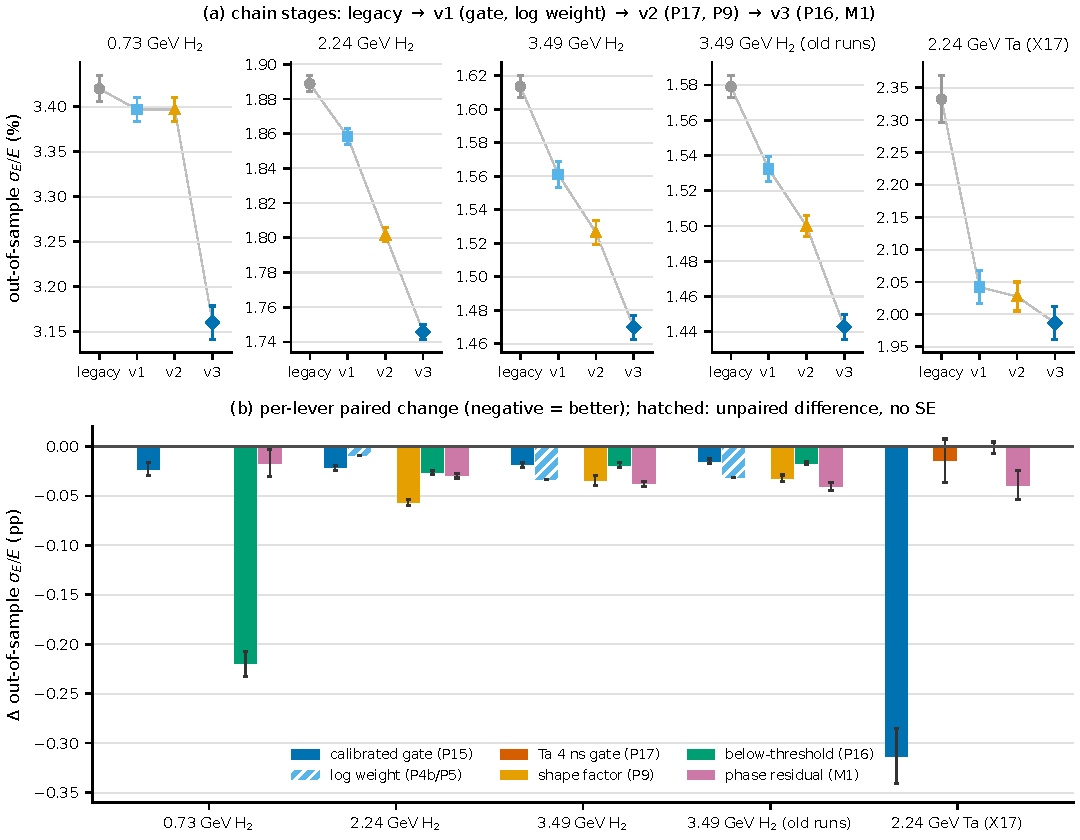
\includegraphics[width=0.95\textwidth]{calib_chain_comparison.pdf}
\caption{Top: out-of-sample $\sigma_E/E$ per run type for the four states of the chain (Table~\ref{tab:calibchains}), with the standard error over splits. Bottom: out-of-sample $\Delta(\sigma_E/E)$ of the levers of Table~\ref{tab:calibattr}, paired with the standard error over pairs; the log-weight bar (hatched) is the unpaired difference of the v1 control and the best-gate value of \code{P5\_latest.tsv} and carries no error. Produced by \code{make\_figs/calib\_figs.py}.}
\label{fig:calibchain}
\end{figure}

\paragraph{Time gate: raw against calibrated times.} The gate scan of 12 November used the raw matched-filter times over 2 to 24\,ns. Its one-standard-error rule chose 11.5 to 13\,ns for the H$_2$ data, while the plain minima lay at 15.5 to 20.5\,ns. With the module offsets subtracted (step~3) the scan was repeated at 1 to 24\,ns (Fig.~\ref{fig:calibgate}). Below 8\,ns the calibrated gate is far better than the raw gate at the same width (at 2.24\,GeV and 4\,ns: 1.921 against 2.146\,\%), and above 8 to 10\,ns the two curves agree within 0.01 percentage points. The steep part of the raw curve was the spread of the module offsets. The control gates are the minima of the calibrated scan (16\,ns; 20\,ns at 0.73\,GeV), chosen over the one-standard-error rule by the decision of 13 November. Figure~\ref{fig:calibdt} shows the seed--member time difference behind this. The raw distribution has a shoulder out to $+8$ to 9\,ns (0.8 to 1.0\,\% of the members between 7 and 10\,ns) that the offsets remove. The late tail (members later than the seed by more than 8\,ns) remains at 0.06, 1.75 and 3.06\,\% of the members at 0.73, 2.24 and 3.49\,GeV and 4.2\,\% for tantalum. For the tantalum data the calibrated gate gains $0.30$ percentage points on the legacy path; the minimum is flat from 3 to 12\,ns and the gate was set to 4\,ns on the tails (\code{P17\_asym\_window.md}). Against 8\,ns, $\sigma_E/E$ is null ($-0.015 \pm 0.022$) while \code{tail\_hi3} falls by $0.25$ (41\,\% of its value), \code{leak\_cut} by 0.42 and the pile-up flag by 0.67 percentage points. The accidental floor of the tantalum runs is four times higher against the peak than in the H$_2$ runs (\code{P17\_asym\_window.md}), so a wide late bound costs more there. On the v3 chain no neighbouring gate beats the control gate by 2 standard errors (\code{control\_phase2\_v3\_gates.tsv}), and the gates stay.

\begin{figure}[htbp]
\centering
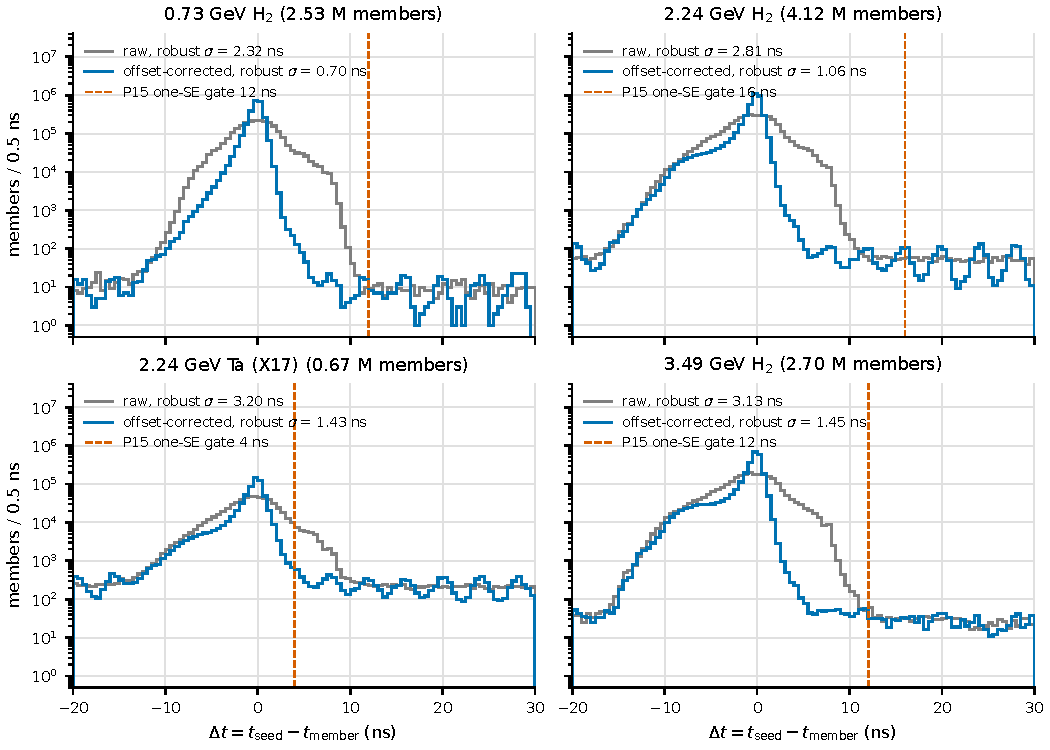
\includegraphics[width=0.95\textwidth]{calib_seed_member_dt.pdf}
\caption{Time difference between the seed and the other members of legacy clusters, raw matched-filter times and times with the module offsets subtracted, per run type (0.5\,ns bins, logarithmic scale; first three splits per run type). Redrawn by \code{make\_figs/calib\_figs.py} from the inputs of \code{improvement/tools/p15\_dt\_hist.py}. The marked gates are those of the one-standard-error rule of the P15 scan (12/16/4/12\,ns), not the control gates.}
\label{fig:calibdt}
\end{figure}

\begin{figure}[htbp]
\centering
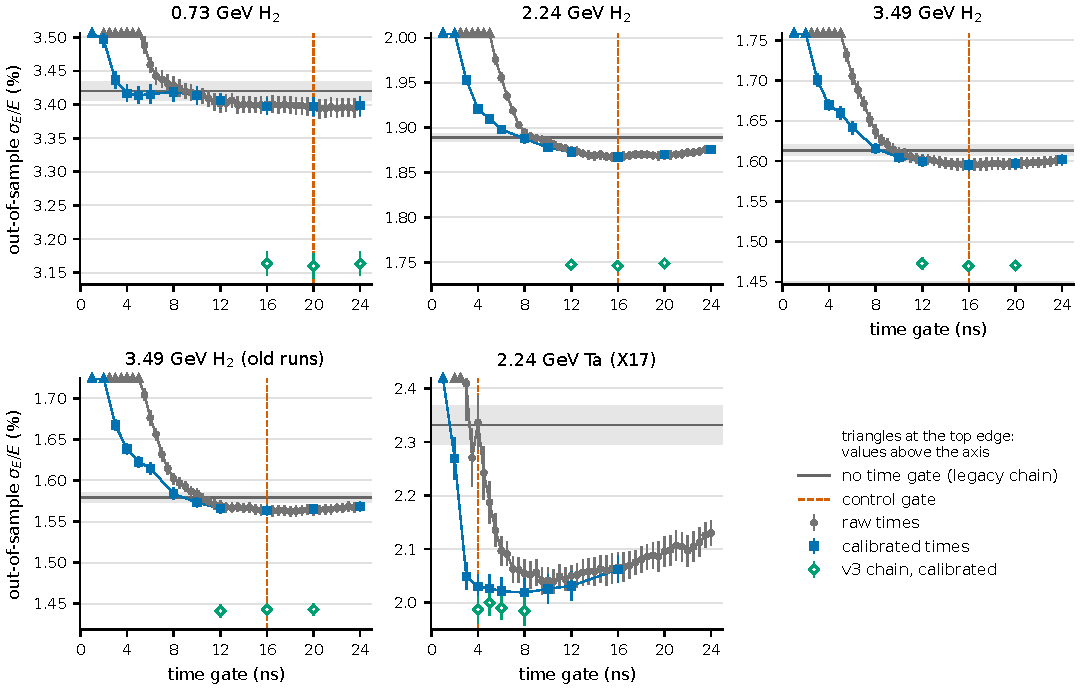
\includegraphics[width=0.95\textwidth]{calib_gate_scan.pdf}
\caption{Out-of-sample $\sigma_E/E$ against the gate width, per run type, with raw matched-filter times (scan of 12 November, \code{energy\_resolution/<RT>/summary.tsv}) and with calibrated times (\code{P15\_tgate\_calibrated.tsv}); both on the legacy corrections. The horizontal line and band are the ungated reference path, the vertical line the control gate of v3, and the open points the v3 chain near it (\code{control\_phase2\_v3\_gates.tsv}). Raw values above the axis range sit as triangles on the top edge. Produced by \code{make\_figs/calib\_figs.py}.}
\label{fig:calibgate}
\end{figure}

\paragraph{Tested and rejected.} Each of the following was measured against the control of its time with the rule of step~15 and is not in the chain (notes \code{P1}, \code{P3}, \code{P4}, \code{P6}, \code{P8}, \code{P11}, \code{P17}). M{\o}ller rejection worsens $\sigma_E/E$ by $0.167 \pm 0.013$ at 0.73\,GeV and $0.009 \pm 0.001$ at 2.24\,GeV and is null at 3.49\,GeV; the non-linearity correction of the calibration files worsens it by $0.095 \pm 0.003$ at 3.49\,GeV, and both stay off. The seed-indexed gain refinement of the previous chain gains $0.03$ (H$_2$) and $0.08$ (tantalum) percentage points in sample and nothing held out ($+0.003 \pm 0.001$ at 2.24\,GeV), so it is a training artefact, and the settings of the member solve (prior, passes, windows, seed fraction) are all null. A candidate separation of 12 instead of 8\,ns in the fitter is null ($-0.0022 \pm 0.0023$ out of sample); the relative amplitude floor \code{R\_MODEL} $= 0.3$ gains $0.030$ at 3.49\,GeV but raises \code{tail\_hi3} and worsens the tantalum data by $0.083 \pm 0.025$. No acceptance rule for secondary pulses passes, because the gated clusterer already absorbs in-gate extras. Asymmetric time windows change the H$_2$ widths by at most 0.0013 percentage points and the tantalum width by $-0.013 \pm 0.007$. Dropping or scaling the lead-glass members is null on the pool and on the T ring; a fiducial cut on the outermost PbWO$_4$ layer would gain 0.20 to 0.43 percentage points on T at the cost of 43 to 47\,\% of its clusters and is kept as an option. Of the earlier chain's 1.794\,\% at 2.24\,GeV, the reconciliation of \code{P1\_reconcile.md} left 0.088 percentage points; \code{P6\_gain\_arm.md} attributes 0.029 of them to the in-sample seed refit of the old chain, and about 0.06 remain unexplained. The old chain, its bank and its tables are no longer on disk.

\subsection{Results of the v3 chain}\label{sec:calibres}

Table~\ref{tab:calibres} lists the v3 values at the control gate (\code{control\_phase2\_v3.md}, \code{control\_phase2\_v3\_delta.tsv}). The v3 change (v3 $-$ v2) meets the rule of step~15 at every run type. The width improves by 2.9 (tantalum) to 22 (2.24\,GeV) standard errors with the same sign in every run. \code{leak\_cut} falls by 0.39, 0.67, 0.68 and 0.24 percentage points at 2.24, 3.49, 3.49\,GeV (earlier) and for tantalum and is null at 0.73\,GeV; \code{tail\_hi\_f} is lower or null, \code{eff\_cut} up or null, and the yield changes by at most $-0.32\,\%$. One guard is waived: at 2.24\,GeV \code{tail\_lo\_f} rises by $0.056 \pm 0.007$ on a tail of 26.9\,\% at the below-threshold step, and the mechanism is not measured. The peak moves by $+0.015\,\%$, because the below-threshold correction adds energy. The two levers that act on the pool add up: the stack total equals the sum of the isolated measurements within 0.002 percentage points at every H$_2$ run type. The below-threshold correction dominates at 0.73\,GeV and the phase residual at 2.24 and 3.49\,GeV; at 0.73\,GeV the phase residual is null in the stack and stays on by decision.

\begin{table}[htbp]
\centering
\caption{v3 at the control gate, pool, out of sample (\code{control\_phase2\_v3.md}): $\sigma_E/E$ in percent, the separation $s_\pi$ and the tail, efficiency and leak fractions in percent as defined in step~14. Yield: peak yield relative to the legacy path. Splits: number of files.}
\label{tab:calibres}
\small
\begin{tabular}{lrlrrrrrr}
\toprule
Run type & Splits & $\sigma_E/E$ & $s_\pi$ & \code{tail\_hi\_f} & \code{tail\_lo\_f} & \code{leak\_cut} & \code{eff\_cut} & Yield \\
\midrule
\code{0p73GeV\_H2} & 16 & $3.160 \pm 0.018$ & 6.29 & 0.001 & 19.58 & 0.01 & 49.4 & 100.66 \\
\code{2p24GeV\_H2} & 42 & $1.746 \pm 0.004$ & 3.70 & 0.068 & 26.94 & 3.78 & 69.6 & 100.55 \\
\code{3p49GeV\_H2} & 16 & $1.470 \pm 0.007$ & 2.83 & 0.226 & 11.82 & 20.96 & 85.3 & 100.52 \\
\code{3p49GeV\_H2}, earlier runs & 28 & $1.443 \pm 0.007$ & 2.88 & 0.189 & 11.30 & 20.66 & 85.8 & 100.41 \\
\code{2p24GeV\_Ta\_X17} & 25 & $1.987 \pm 0.025$ & 3.27 & 0.287 & 45.10 & 4.49 & 51.2 & 103.18 \\
\bottomrule
\end{tabular}
\end{table}

Figure~\ref{fig:calibpeak} shows the elastic peak at 3.49\,GeV on the legacy path and on the v3 chain.

\begin{figure}[htbp]
\centering
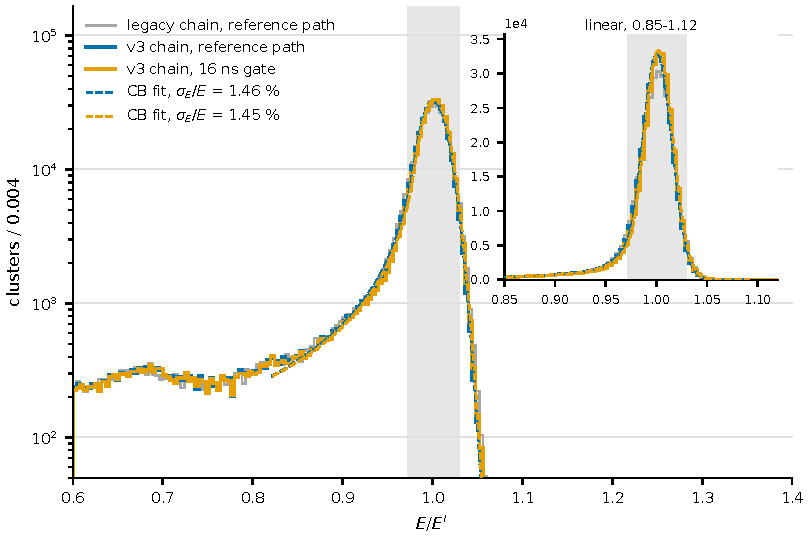
\includegraphics[width=0.8\textwidth]{calib_elastic_peak_3p49gev_h2.pdf}
\caption{Cluster energy over the elastic reference energy, $E/E'$, for \code{3p49GeV\_H2} (runs 24698 and 24911; all files pooled; in sample). Blue: v3 chain on the ungated reference path; orange: v3 chain at the 16\,ns gate; thin grey: the legacy chain of 12 November (with run 24937), whose pooled fit gives 1.58\,\%. Dashed lines: single Crystal Ball fits of the pooled v3 histograms, with $\sigma_E/E$ of 1.46 and 1.45\,\% in the legend. The grey band marks the fitted peak $\pm 2\sigma$ of the blue histogram. The inset shows $0.85 \le E/E' \le 1.12$ on a linear scale. The pooled fit is an illustration; Table~\ref{tab:calibres} quotes the mean over files. Produced by \code{make\_figs/calib\_figs.py} from \code{control\_phase2\_v3\_20261114/v3/3p49GeV\_H2/spectra.npz}.}
\label{fig:calibpeak}
\end{figure}

\paragraph{Tantalum.} The tantalum data take the phase residual (own table, fitted on the chain without the below-threshold correction) and the 4\,ns gate, but no below-threshold table and no ring constants. A tantalum table was built with the tantalum thresholds (median 8.7\,MeV against 9.5\,MeV for \code{2p24GeV\_H2}) on $1.4 \times 10^4$ peak clusters per half. It narrows the peak by $0.077 \pm 0.015$ percentage points and lowers \code{leak\_cut} by 0.50, but \code{tail\_lo\_f} rises by $0.86 \pm 0.08$ and \code{eff\_cut} falls by $0.64 \pm 0.09$, both at 8 to 11 standard errors, so it is not adopted; the tables are kept under \code{prep/below\_thr\_Ta/}. The 2.24\,GeV position map that the tantalum data borrow changed with the below-threshold correction, and that change alone is null on tantalum in every column.

\paragraph{Rings.} Outside the pool the ring constants of step~11 act where the gain solve of the pool left modules on the prior. Table~\ref{tab:calibrings} gives the trained rings. The H ring, which holds the modules around the beam hole, gains 0.34 to 0.89 percentage points from v2 to v3, of which 0.26 to 0.80 come from the ring solve; the M ring gains 0.10 to 0.69. The ring steps are 5 to 15\,\% smaller than the ring solve measured alone on v2 (H: $-0.26$ against $-0.30$, $-0.65$ against $-0.69$, $-0.80$ against $-0.85$), and the 2.24\,GeV M step is half of it ($-0.031$ against $-0.059$). Two causes are plausible and not separated: the below-threshold correction already absorbs part of a per-module scale, and the v3 training set lacks the O and T clusters of the P7 measurement. The out-of-sample minus in-sample gap of the rings changes by $-0.13$ to $+0.30$ percentage points (it rises on five of the six rings), which the adoption rule for ring-only constants waives; the gap of the pool does not change. The O and T rings stay on the pool constants: the ring solve was null there, and the constants from the snake-scan and cosmic data are not yet available (Section~\ref{sec:calibopen}).

\begin{table}[htbp]
\centering
\caption{Ring rows of v3, out of sample (\code{control\_phase2\_v3.md}; legacy region values from \code{P2\_regions.md}): $\sigma_E/E$ in percent on the legacy path with the pool constants and on v3 with the ring constants; the paired change from v2 to v3 and the part of it from the ring solve. The pool values of v3 are those of Table~\ref{tab:calibres}.}
\label{tab:calibrings}
\small
\begin{tabular}{llllll}
\toprule
Run type & Ring & Legacy & v3 & v3 $-$ v2 & of which ring solve \\
\midrule
\code{0p73GeV\_H2} & M & -- & 3.444 & $-0.685 \pm 0.049$ & $-0.461 \pm 0.046$ \\
\code{2p24GeV\_H2} & H & 2.365 & 1.822 & $-0.338 \pm 0.008$ & $-0.262 \pm 0.008$ \\
\code{2p24GeV\_H2} & M & 2.043 & 1.871 & $-0.096 \pm 0.010$ & $-0.031 \pm 0.009$ \\
\code{3p49GeV\_H2} & H & 2.411 & 1.663 & $-0.725 \pm 0.009$ & $-0.648 \pm 0.013$ \\
\code{3p49GeV\_H2}, earlier runs & H & -- & 2.187 & $-0.893 \pm 0.048$ & $-0.804 \pm 0.052$ \\
\code{3p49GeV\_H2}, earlier runs & M & -- & 1.788 & $-0.219 \pm 0.030$ & $-0.183 \pm 0.036$ \\
\bottomrule
\end{tabular}
\end{table}

\paragraph{Resolution against energy.} The form $\sigma_E/E = a_E \oplus b_E/\sqrt{E} \oplus c_E/E$ fitted to the three out-of-sample H$_2$ values of Table~\ref{tab:calibres} at the control gate gives $a_E = 0.89 \pm 0.05\,\%$, $b_E = 2.06 \pm 0.07\,\%\,\mathrm{GeV}^{1/2}$ and $c_E = 1.34 \pm 0.07\,\%\,\mathrm{GeV}$ (\code{resfit.out} of the v3 run directory; Fig.~\ref{fig:calibfit}), against $1.10 \oplus 1.99 \oplus 1.62$ on the best-gate values of 12 November. The fit has three points and three parameters, so its coefficients carry no test of the form, and with zero degrees of freedom the terms trade against each other. The sources of the change are nevertheless known: the fall of $c_E$ is the below-threshold correction at 0.73\,GeV, which removes a fluctuation that scales like a noise term, and the fall of $a_E$ is the phase residual, the below-threshold correction and the shape factor at 2.24 and 3.49\,GeV. The two-term form gives $\chi^2 = 84$ for one degree of freedom and is rejected. With the earlier 3.49\,GeV runs as a fourth point the fit gives $0.81 \oplus 2.16 \oplus 1.25$ with $\chi^2 = 6.9$ for one degree of freedom, because the two 3.49\,GeV sets differ by $0.027 \pm 0.010$ percentage points. The tantalum point is excluded, as before. For comparison, the PRad-II proposal (arXiv:2009.10510) quotes $2.6\,\%/\sqrt{E}$, which gives 3.05, 1.74 and 1.39\,\% at the three beam energies, and the PrimEx data shown in the X17 proposal (arXiv:2108.13276, Fig.~14) follow $1.13 \oplus 1.73/\sqrt{E} \oplus 1.77/E$ percent, which gives 3.36, 1.80 and 1.55\,\%. The v3 values are below the PrimEx curve at all three energies and within 0.11, 0.01 and 0.08 percentage points of the proposal curve.

\begin{figure}[htbp]
\centering
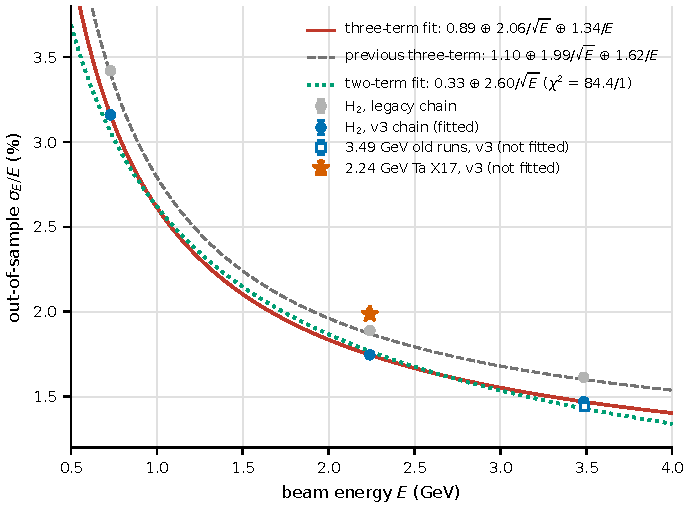
\includegraphics[width=0.7\textwidth]{calib_resolution_vs_energy.pdf}
\caption{Out-of-sample $\sigma_E/E$ at the control gate versus beam energy on the v3 chain. Blue points: H$_2$ runs at 0.73, 2.24 and 3.49\,GeV, with the standard error over files; open point: the earlier 3.49\,GeV runs; orange star: \code{2p24GeV\_Ta\_X17}; grey points: legacy path. Red line: three-term fit to the three blue points (zero degrees of freedom); grey dashed line: the three-term fit of 12 November; green dotted line: two-term fit ($\chi^2/\mathrm{dof} = 84/1$). Produced by \code{make\_figs/calib\_figs.py}.}
\label{fig:calibfit}
\end{figure}

\paragraph{Budget at 3.49\,GeV.} The budget of \code{P5\_budget.md} was assembled on the legacy path in sample (1.585\,\%), where the excess over the $2.6\,\%/\sqrt{E}$ stochastic term (1.39\,\%) is 0.76\,\% or $0.57\,\%^2$ in quadrature. Its measured rows are the calibrated gate ($0.25\,\%$ in quadrature), the log weight ($0.28\,\%$), an upper bound for the edge dependence ($0.38\,\%$), the threshold loss ($0.42\,\%$, model-dependent, 0.29 to 0.69\,\%) and the non-linearity and M{\o}ller switches (no lever); noise, template scatter and crosstalk ($0.04$ to $0.12$, about 0.15 and 0.08\,\%) are inferred, and the LMS drift is null. Of the $0.57\,\%^2$, the measured levers account for 0.19, the edge bound for 0.14 and the threshold term for 0.17, leaving $0.07\,\%^2$. The v3 chain has since acted on the gate, log-weight, edge and threshold rows and added the phase residual; in quadrature it removed $\sqrt{1.585^2 - 1.445^2} = 0.65\,\%$ in sample and $\sqrt{1.614^2 - 1.470^2} = 0.67\,\%$ out of sample, and the out-of-sample excess over the stochastic term is now $\sqrt{1.470^2 - 1.39^2} = 0.48\,\%$ (arithmetic on Table~\ref{tab:calibchains}). A re-measured budget on the v3 basis does not exist.

\subsection{Open items}\label{sec:calibopen}

\begin{enumerate}
\item The O and T rings keep the pool constants. Their calibration needs the snake-scan and cosmic data. The snake scan moved the calorimeter through a 2108.85\,MeV bremsstrahlung beam (runs 23699 to 23720 for the PbWO$_4$ part, 23721 to 23723 for the lead glass). Cosmic runs exist after the scan (23741, 23743 to 23745), during the 3.49\,GeV period (13 runs between 24154 and 24422) and during the 0.73\,GeV period (24617). All are stored at JLab only, and none has been decoded. The snake scan would also give a fourth energy point for the three-term fit (2.11\,GeV, next to 2.24\,GeV, so a weak constraint on $c_E$).
\item The ring constants of step~11 have no production consumer: a per-cluster lookup of the seed ring is needed before they can be used outside the benchmark.
\item The tantalum data have no below-threshold table. The own table fails the low-side guards, and the cause (a heavier radiative tail, or threshold classes set for H$_2$ while most tantalum modules fall below 9.0\,MeV) is not investigated.
\item The 0.73\,GeV data have no position correction. Part of the below-threshold gain there acts as the missing correction, and a position-correction arm on the v3 chain is untested.
\item The mechanism of the waived \code{tail\_lo\_f} guard at 2.24\,GeV (Section~\ref{sec:calibres}) is not measured.
\item The two candidate causes of the 2.24\,GeV M-ring step being half of the ring solve alone (Section~\ref{sec:calibres}) are not separated.
\item The resolution function has zero degrees of freedom (Section~\ref{sec:calibres}).
\item The phase-residual tables assume the banks of the scans ($t_{50}$) and must be refitted when a bank or the onset definition changes; the below-threshold tables must be refitted when the thresholds change. \code{poscorr\_comparison.py} clusters events on its own and sees neither table.
\item The lead glass has no calibration, and the layer-0 fiducial cut on T (Section~\ref{sec:calibcomp}) is an acceptance decision not yet taken.
\end{enumerate}

\clearpage
\appendix

\section{Constants of the pile-up fitter}
\label{app:const}

Table~\ref{tab:mfconst} lists the constants of the class \code{MF} of Section~\ref{sec:fitter}. The values are the same in \code{pileup\_deconvolution\_study.py}, \code{pileup\_rates.py}, \code{crosstalk\_study.py} and the committed \code{energy\_resolution\_benchmark.py}.

\begin{table}[htbp]
\centering
\caption{Constants of the pile-up fitter. The last three rows belong to the wrapper used by the scans of data.}
\label{tab:mfconst}
\small
\begin{tabular}{lll}
\toprule
Constant & Value & Role \\
\midrule
\code{PED\_NSAMPLES} & 30 samples & baseline and noise window (samples 0 to 29) \\
\code{SIGMA\_MIN} & 0.3\,ADC & floor of the noise estimate \\
\code{CAND\_NSIGMA} & 3 & pre-selection of a waveform, in units of $\sigma$ (floor 3\,ADC) \\
\code{OVERFLOW} & 4095\,ADC & a sample at or above this value is clipped \\
\code{DT}, \code{NPH} & 4\,ns, 4 & sample period; onset phases of the kernel (1\,ns steps) \\
\code{L} & 24 samples & length of the matched-filter kernel (96\,ns) \\
\code{LW}, \code{LEAD} & 32, 3 samples & fit window of a pulse; samples before the onset \\
\code{LUT\_DT} & 0.05\,ns & step of the template table \\
\code{KMAX} & 6 & largest number of pulses of a waveform \\
\code{NSIGMA} & 5 & significance of a candidate and of a fitted pulse \\
\code{MIN\_AMP} & 5\,ADC & amplitude floor of a candidate \\
\code{PEAK\_SMOOTH\_NS} & 8\,ns & width of the Gaussian smoothing of stage A \\
\code{PEAK\_FRAC} & 0.02 & stage A: smoothed height relative to the highest candidate \\
\code{MIN\_SEP\_NS} & 8\,ns & smallest distance between two candidates (stages A and C) \\
\code{MERGE\_NS} & 6.5\,ns & fitted pulses closer than this are merged \\
\code{R\_MODEL} & 0.02 & stage C: amplitude relative to the largest pulse within 96\,ns \\
\code{BIC\_PENALTY} & 1 & stage C: factor on $2 \ln n_{\mathrm{fit}}$ in Eq.~\eqref{eq:bic} \\
\code{SHAPE\_SIGMA\_MIN} & 0.005 & floor of the shape scatter $\sigma_s$ \\
\code{A\_MIN\_SCALE} & 20\,ADC & floor of the amplitude in the scaling of $\sigma_s$ \\
\code{BASE\_CLIP} & 1 & limit of the baseline offset $\delta p$, in units of $\sigma$ \\
\code{RAW\_NSIGMA} & 5 & raw height of a pulse above the baseline, in units of $\sigma$ \\
\code{LATE\_MIN\_TAIL} & 6 samples & samples required after the peak of a late pulse \\
\midrule
\code{N\_REF\_EVENTS} & 20\,000 & events of a file used for the noise reference \\
\code{MIN\_REF\_WAVEFORMS} & 20 & smallest number of reference waveforms of a module \\
\code{START\_NSIGMA} & 3 & baseline start replaced by $p_{\mathrm{ref}}$ beyond this distance, in units of $\sigma_{\mathrm{ref}}$ \\
\bottomrule
\end{tabular}
\end{table}

Two values rest on tests recorded in the comments of the code, without an output file. With a baseline limit of $3\sigma$ the control events of Section~\ref{sec:deconv} had a false-positive rate of 0.42\,\%, against 0.08\,\% with $1\sigma$. Values of \code{BIC\_PENALTY} from 1 to 3 gave the same efficiencies.

\section{Hot modules}
\label{app:hot}

Table~\ref{tab:hot} lists the eight modules of largest cut rate per run type (Section~\ref{sec:rates}, step 13), from the first page of \code{hot\_modules.pdf}. None of them has a dead neighbour.

\begin{table}[htbp]
\centering
\caption{Hot modules: the eight modules of largest cut rate $F$ per run type, among the modules with at least 100 channels above threshold. $x$, $y$: module centre; ring: $\lfloor \max(|x|, |y|) / d \rfloor$ with $d$ the module size; $N_{\mathrm{thr}}$, $N_{\mathrm{cut}}$ and the binomial error as in Eq.~\eqref{eq:rate}. Template: e = own, elastic pool; g = own, general pool; s = single pulse; a = run-type average.}
\label{tab:hot}
\footnotesize
\begin{tabular}{rlrrrrrrl}
\toprule
Rank & Module & $x$ (mm) & $y$ (mm) & Ring & $N_{\mathrm{thr}}$ & $N_{\mathrm{cut}}$ & $F$ (\%) & Template \\
\midrule
\multicolumn{9}{l}{\code{2p24GeV\_Ta\_X17}} \\
1 & W563 & 31 & 10 & 1 & 97\,691 & 31\,559 & $32.30 \pm 0.15$ & e \\
2 & W528 & 10 & 31 & 1 & 87\,344 & 27\,502 & $31.49 \pm 0.16$ & e \\
3 & W527 & $-10$ & 31 & 1 & 73\,770 & 21\,544 & $29.20 \pm 0.17$ & e \\
4 & W560 & $-31$ & 10 & 1 & 66\,573 & 19\,359 & $29.08 \pm 0.18$ & e \\
5 & W630 & 10 & $-31$ & 1 & 64\,035 & 18\,336 & $28.63 \pm 0.18$ & e \\
6 & W597 & 31 & $-10$ & 1 & 72\,666 & 20\,780 & $28.60 \pm 0.17$ & e \\
7 & W629 & $-10$ & $-31$ & 1 & 59\,033 & 16\,022 & $27.14 \pm 0.18$ & e \\
8 & W594 & $-31$ & $-10$ & 1 & 60\,081 & 15\,608 & $25.98 \pm 0.18$ & e \\
\midrule
\multicolumn{9}{l}{\code{0p73GeV\_H2}} \\
1 & W335 & 239 & 156 & 11 & 214 & 208 & $97.20 \pm 1.13$ & s \\
2 & W1022 & $-322$ & $-280$ & 15 & 108 & 7 & $6.48 \pm 2.37$ & s \\
3 & W944 & 177 & $-218$ & 10 & 174 & 10 & $5.75 \pm 1.76$ & a \\
4 & W176 & $-239$ & 239 & 11 & 131 & 7 & $5.34 \pm 1.96$ & e \\
5 & W1082 & 218 & $-301$ & 14 & 101 & 4 & $3.96 \pm 1.94$ & e \\
6 & W367 & 197 & 135 & 9 & 380 & 15 & $3.95 \pm 1.00$ & e \\
7 & W678 & 301 & $-52$ & 14 & 178 & 7 & $3.93 \pm 1.46$ & g \\
8 & W782 & 343 & $-114$ & 16 & 158 & 6 & $3.80 \pm 1.52$ & e \\
\midrule
\multicolumn{9}{l}{\code{2p24GeV\_H2}} \\
1 & W1 & $-343$ & 342 & 16 & 318 & 159 & $50.00 \pm 2.80$ & e \\
2 & W950 & 301 & $-218$ & 14 & 221 & 72 & $32.58 \pm 3.15$ & g \\
3 & W1145 & 114 & $-342$ & 16 & 239 & 77 & $32.22 \pm 3.02$ & e \\
4 & W309 & $-301$ & 156 & 14 & 475 & 112 & $23.58 \pm 1.95$ & e \\
5 & W62 & 218 & 322 & 15 & 101 & 22 & $21.78 \pm 4.11$ & g \\
6 & W818 & $-322$ & $-156$ & 15 & 230 & 40 & $17.39 \pm 2.50$ & e \\
7 & W307 & $-343$ & 156 & 16 & 247 & 30 & $12.15 \pm 2.08$ & g \\
8 & W545 & $-343$ & 10 & 16 & 732 & 69 & $9.43 \pm 1.08$ & g \\
\midrule
\multicolumn{9}{l}{\code{3p49GeV\_H2}} \\
1 & W121 & 31 & 280 & 13 & 268 & 19 & $7.09 \pm 1.57$ & e \\
2 & W335 & 239 & 156 & 11 & 136 & 7 & $5.15 \pm 1.89$ & g \\
3 & W480 & $-280$ & 52 & 13 & 273 & 14 & $5.13 \pm 1.33$ & g \\
4 & W910 & 177 & $-197$ & 9 & 261 & 6 & $2.30 \pm 0.93$ & e \\
5 & W937 & 31 & $-218$ & 10 & 1501 & 31 & $2.07 \pm 0.37$ & e \\
6 & W812 & 260 & $-135$ & 12 & 104 & 2 & $1.92 \pm 1.35$ & e \\
7 & W439 & 280 & 93 & 13 & 109 & 2 & $1.83 \pm 1.29$ & e \\
8 & W299 & 197 & 176 & 9 & 303 & 4 & $1.32 \pm 0.66$ & e \\
\bottomrule
\end{tabular}
\end{table}

\end{document}
